\PassOptionsToPackage{dvipsnames}{xcolor}
\documentclass[UTF8,12pt]{ctexart}

% 显式给 Fandol 中文字体登记 small-caps 形状。
% 模板的 \ChapterSectionLabel 与 titlepage 都用到 \textsc / \scshape，
% 默认查不到 CJK 字体的 sc 形状会出现 "Font shape ... sc undefined" 警告；
% 这里把 sc 显式落到 Regular/Hei，警告消失，输出无可见变化（中文本无大小写之分）。
\setCJKmainfont{FandolSong-Regular}[
  Extension  = .otf,
  ItalicFont = FandolKai-Regular,
  BoldItalicFont = FandolKai-Regular,
  Script = Default,
  BoldFont   = FandolHei-Regular,
  FontFace   = {m}{sc}{Font=FandolSong-Regular},
  FontFace   = {bx}{sc}{Font=FandolHei-Regular},
]

\usepackage[paper=a4paper,left=2.5cm,right=2.5cm,top=3cm,bottom=3cm]{geometry}
\usepackage{amsmath,amsthm,amssymb,mathrsfs,bbm,needspace}
\usepackage{graphicx,tikz-cd,titlesec}
\usepackage[dvipsnames]{xcolor}
\usepackage[
    colorlinks=true,
    linkcolor=MidnightBlue,
    citecolor=BrickRed,
    urlcolor=MidnightBlue,
    linktoc=all
]{hyperref}

\pagestyle{plain}

% 设置环境
\usepackage{aliascnt}
\theoremstyle{plain}
\newtheorem{theorem}{定理}[section]
\newaliascnt{definition}{theorem}
\newtheorem{definition}[definition]{定义}
\aliascntresetthe{definition}
\newaliascnt{lemma}{theorem}
\newtheorem{lemma}[lemma]{引理}
\aliascntresetthe{lemma}
\newaliascnt{corollary}{theorem}
\newtheorem{corollary}[corollary]{推论}
\aliascntresetthe{corollary}
\newaliascnt{remark}{theorem}
\newtheorem{remark}[remark]{注}
\aliascntresetthe{remark}
\newaliascnt{example}{theorem}
\newtheorem{example}[example]{例}
\aliascntresetthe{example}
\newaliascnt{proposition}{theorem}
\newtheorem{proposition}[proposition]{命题}
\aliascntresetthe{proposition}
\newaliascnt{problem}{theorem}
\newtheorem{problem}[problem]{问题}
\aliascntresetthe{problem}
\newtheorem{exercise}{习题}
\numberwithin{equation}{section}
\numberwithin{figure}{section}

% autoref names
\providecommand{\sectionautorefname}{章}
\renewcommand{\sectionautorefname}{章}

\providecommand{\subsectionautorefname}{节}
\renewcommand{\subsectionautorefname}{节}

\providecommand{\definitionautorefname}{定义}
\renewcommand{\definitionautorefname}{定义}

\providecommand{\theoremautorefname}{定理}
\renewcommand{\theoremautorefname}{定理}

\providecommand{\lemmaautorefname}{引理}
\renewcommand{\lemmaautorefname}{引理}

\providecommand{\propositionautorefname}{命题}
\renewcommand{\propositionautorefname}{命题}

\providecommand{\corollaryautorefname}{推论}
\renewcommand{\corollaryautorefname}{推论}

\providecommand{\exampleautorefname}{例}
\renewcommand{\exampleautorefname}{例}

\providecommand{\remarkautorefname}{注}
\renewcommand{\remarkautorefname}{注}

\providecommand{\exerciseautorefname}{习题}
\renewcommand{\exerciseautorefname}{习题}

\providecommand{\problemautorefname}{问题}
\renewcommand{\problemautorefname}{问题}

\providecommand{\figureautorefname}{图}
\renewcommand{\figureautorefname}{图}

\providecommand{\tableautorefname}{表}
\renewcommand{\tableautorefname}{表}

% 设置 proof 样式
\makeatletter
\renewcommand{\proofname}{\textbf{证明}}
\renewenvironment{proof}[1][\proofname]{\par
  \pushQED{\qed}%
  \normalfont
  \topsep6\p@\@plus6\p@\relax
  \trivlist
  \item[\hskip\labelsep
        \normalfont\bfseries
    #1\@addpunct{.}]\ignorespaces
}{%
  \popQED\endtrivlist\@endpefalse
}
\makeatother
\renewcommand{\qedsymbol}{\ensuremath{\square}}

% 设置 section 样式
\newlength{\chapterNumSpace}
\setlength{\chapterNumSpace}{1.4cm}

% 附录判断：正文显示 Chapter，\appendix 后显示 Appendix
\newif\ifInAppendix
\InAppendixfalse

% 目录中的附录判断
\newif\ifInAppendixToc
\InAppendixTocfalse

% 目录可调参数
\newlength{\tocSectionLabelWidth}
\setlength{\tocSectionLabelWidth}{4.2em}

\newlength{\tocAppendixGap}
\setlength{\tocAppendixGap}{0.2em}

\newlength{\tocSubIndent}
\setlength{\tocSubIndent}{1.2em}

\newlength{\tocSubNumWidth}
\setlength{\tocSubNumWidth}{3.0em}

% 目录 section 编号文字
\newcommand{\TocSectionNumber}[1]{%
  \ifInAppendixToc
    附录\hspace{\tocAppendixGap}#1%
  \else
    第~#1~章%
  \fi
}

\makeatletter

% section 目录格式：
% 正文：第 1 章 群的定义与性质
% 附录：附录A 集合论补遗
\renewcommand*\l@section[2]{%
  \ifnum\c@tocdepth>\z@
    \addvspace{0.55em}%
    \begingroup
      \parindent\z@
      \rightskip\@pnumwidth
      \parfillskip-\@pnumwidth
      \leavevmode
      \bfseries
      \setlength{\@tempdima}{\tocSectionLabelWidth}%
      \advance\leftskip\@tempdima
      \hskip-\leftskip
      \def\numberline##1{%
        \makebox[\@tempdima][l]{\TocSectionNumber{##1}}%
      }%
      #1\nobreak\hfill\nobreak\makebox[\@pnumwidth][r]{#2}\par
    \endgroup
  \fi
}

% subsection 目录格式：
% 1.1 循环群 / A.1 集合基础
\renewcommand*\l@subsection{%
  \@dottedtocline{2}{\tocSubIndent}{\tocSubNumWidth}%
}

\makeatother

\let\OriginalAppendix\appendix
\renewcommand{\appendix}{%
  \OriginalAppendix
  \InAppendixtrue
  \addtocontents{toc}{\protect\InAppendixToctrue}%
}

\newcommand{\ChapterSectionLabel}{%
  \thispagestyle{plain}%
  \vspace*{-0.5cm}%
  \makebox[\textwidth][r]{%
    {\fontsize{18pt}{18pt}\selectfont\scshape
      \ifInAppendix 附录\else 第\fi
    }\enspace
    {\fontsize{62pt}{62pt}\selectfont\bfseries\thesection}\enspace{\fontsize{18pt}{18pt}\selectfont\ifInAppendix\else 章\fi}%
  }%
  \par\vspace{-0.25cm}%
  \noindent\rule{\dimexpr\textwidth-\chapterNumSpace\relax}{0.45pt}%
}

\titleformat{\section}[display]
  {\normalfont}
  {\ChapterSectionLabel}
  {0cm}
  {\raggedleft\rightskip=\chapterNumSpace\fontsize{30pt}{35pt}\selectfont\bfseries}
  [\vspace{0.3cm}]

\newcommand{\sectionbreak}{\clearpage}

% 不编号 section，例如前言、目录
\titleformat{name=\section,numberless}[block]
  {\normalfont\Large\bfseries\centering}
  {}
  {0pt}
  {}

% section 整体间距
\titlespacing{\section}
  {0pt}
  {0pt}
  {0pt}

% subsection 样式
\ctexset{
  subsection = {
    format = \large\bfseries
  }
}


\newcommand{\externalref}[2]{\href[page=#1]{../../books/Statistical Optimal Transport.pdf}{#2}}
\providecommand{\subsubsectionautorefname}{节}
\renewcommand{\subsubsectionautorefname}{节}
\renewcommand{\refname}{参考文献}
\hypersetup{pdftitle={统计最优传输：完整中文译稿},pdfauthor={Sinho Chewi; Jonathan Niles-Weed; Philippe Rigollet},bookmarksnumbered=true}



% FULL BOOK EXTENSIONS
\usepackage{wrapfig,multicol,makeidx,xurl}
\setlength{\emergencystretch}{1em}
\newaliascnt{assumption}{theorem}
\newtheorem{assumption}[assumption]{假设}
\aliascntresetthe{assumption}
\providecommand{\assumptionautorefname}{假设}
\newtheorem*{remark*}{注}
\makeatletter
\@addtoreset{exercise}{section}
\@addtoreset{footnote}{section}
\providecommand{\theHexercise}{\thesection.\arabic{exercise}}
\renewcommand{\theHexercise}{\thesection.\arabic{exercise}}
\makeatother
\makeindex
\providecommand{\appendixautorefname}{附录}
\renewcommand{\appendixautorefname}{附录}
\renewcommand{\indexname}{索引}
\renewcommand{\seename}{见}
\makeatletter
\renewenvironment{theindex}{%
  \clearpage\phantomsection\section*{索引}\label{sec:index}%
  \addcontentsline{toc}{section}{索引}%
  \@mkboth{索引}{索引}\thispagestyle{plain}%
  \parindent\z@\parskip\z@\@plus.3\p@\relax%
  \columnsep 28\p@\columnseprule\z@\let\item\@idxitem%
  \begin{multicols}{2}\small%
}{\end{multicols}}
\makeatother

\begin{document}
\hypersetup{pageanchor=false}
\begin{titlepage}
\flushleft
\rule{\textwidth}{1.2pt}\\[0.1cm]
\rule{\textwidth}{0.8pt}\\[1.4cm]
{\fontsize{40pt}{52pt}\selectfont\bfseries 统计最优传输}\\[0.8cm]
{\fontsize{22pt}{30pt}\selectfont\textit{Statistical Optimal Transport}}\\[1.0cm]
\rule{\textwidth}{0.6pt}\\[1.0cm]
{\Large 圣弗卢尔概率论暑期学校\\[0.3cm]第XLIX届——2019年}\\[1cm]
{\large Sinho Chewi\\[0.15cm]Jonathan Niles-Weed\\[0.15cm]Philippe Rigollet}\\[1.2cm]
{\small Lecture Notes in Mathematics 2364；Springer，2025.\\
本稿为学习用完整中文译稿，原书版权归原权利人.\\
章节、陈述、公式、图及习题编号沿用原书.\\
来源疑误照录并另记于随附核验说明.}
\vfill
\begin{flushright}{\small 中文译稿整理于2026年11月3日}\end{flushright}
\end{titlepage}
\pagenumbering{roman}\hypersetup{pageanchor=true}
\clearpage
\thispagestyle{empty}
\begin{center}
{\Large 数学讲义丛书\\[0.5cm]Lecture Notes in Mathematics}\\[0.8cm]
{\Large\bfseries 圣弗卢尔概率论暑期学校}\\[0.3cm]
École d’Été de Probabilités de Saint-Flour\\[0.7cm]
第2364卷
\end{center}
\vspace{0.7cm}
\noindent\textbf{主编}

Jean-Michel Morel，中国香港九龙塘，香港城市大学\par
Bernard Teissier，法国巴黎，IMJ-PRG

\vspace{0.4cm}
\noindent\textbf{丛书编委}

Karin Baur，英国利兹，利兹大学\par
Michel Brion，法国格勒诺布尔，格勒诺布尔阿尔卑斯大学（UGA）\par
Rupert Frank，德国慕尼黑，慕尼黑大学（LMU）\par
Annette Huber，德国弗赖堡，弗赖堡大学\par
Davar Khoshnevisan，美国犹他州盐湖城，犹他大学\par
Ioannis Kontoyiannis，英国剑桥，剑桥大学\par
Angela Kunoth，德国科隆，科隆大学\par
Ariane Mézard，法国巴黎，IMJ-PRG\par
Mark Podolskij，卢森堡埃施，卢森堡大学\par
Mark Policott，英国考文垂，华威大学数学研究所\par
László Székelyhidi，德国莱比锡，马克斯·普朗克数学科学研究所\par
Gabriele Vezzosi，意大利佛罗伦萨，佛罗伦萨大学（UniFI）\par
Anna Wienhard，德国莱比锡，马克斯·普朗克数学科学研究所

\clearpage
\thispagestyle{empty}
\section*{圣弗卢尔概率论暑期学校}

\begin{wrapfigure}{r}{.22\textwidth}
\centering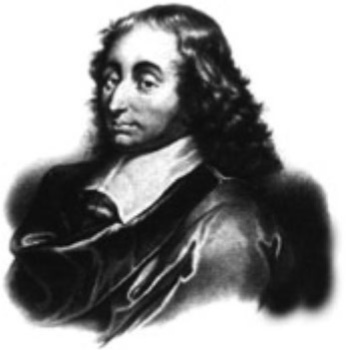
\includegraphics[width=.20\textwidth]{assets/front/saint-flour-portrait.png}
\end{wrapfigure}
圣弗卢尔系列卷册反映了圣弗卢尔概率论暑期学校的授课内容. 暑期学校创办于1971年，每年由法国克莱蒙费朗的布莱兹·帕斯卡数学实验室组织，该实验室隶属于法国国家科学研究中心（CNRS）和克莱蒙奥弗涅大学. 学校面向对概率论、统计学及其应用感兴趣的博士生、教师和研究人员.

学校持续12天（2005年以前为17天），最多接收100名参与者. 期间开设三门高水平课程，对概率论或统计学的某些领域作全面深入的研究. 讲师均由国际科学委员会选定. 参与者还有机会围绕自己的研究工作作简短报告.

参与者在同一栋建筑内住宿和学习. 这是一所位于圣弗卢尔市、建于18世纪的旧神学院，海拔900米. 宜人的环境有利于科学讨论与交流.

圣弗卢尔概率论暑期学校获得以下机构支持：
\begin{itemize}
\item 布莱兹·帕斯卡数学实验室；
\item 克莱蒙奥弗涅大学；
\item 法国国家科学研究中心（C.N.R.S.）；
\item 欧洲数学学会（E.M.S.）.
\end{itemize}
更多信息见：\url{https://lmbp.uca.fr/stflour/stflour-en.php}

\noindent\textbf{Christophe Bahadoran}\par
\href{mailto:Christophe.Bahadoran@uca.fr}{Christophe.Bahadoran@uca.fr}

\noindent\textbf{Arnaud Guillin}\par
\href{mailto:Arnaud.Guillin@uca.fr}{Arnaud.Guillin@uca.fr}

\noindent\textbf{Hacène Djellout}\par
\href{mailto:Hacene.Djellout@uca.fr}{Hacene.Djellout@uca.fr}

\href{mailto:stflour.lmbp@uca.fr}{stflour.lmbp@uca.fr}\par
法国克莱蒙奥弗涅大学，Aubière cedex

\clearpage
\thispagestyle{empty}
\noindent Sinho Chewi\enspace$\bullet$\enspace Jonathan Niles-Weed\enspace$\bullet$\enspace Philippe Rigollet
\vspace{3cm}
\begin{center}
{\Huge\bfseries 统计最优传输}\\[0.8cm]
{\Large Statistical Optimal Transport}\\[1cm]
{\Large 圣弗卢尔概率论暑期学校\\[0.3cm]第XLIX届——2019年}\\[0.5cm]
École d’Été de Probabilités de Saint-Flour XLIX -- 2019
\end{center}
\vfill
\noindent Springer

\clearpage
\thispagestyle{empty}
{\small
\noindent\textbf{Sinho Chewi}\par
美国康涅狄格州纽黑文，耶鲁大学统计与数据科学系

\noindent\textbf{Jonathan Niles-Weed}\par
美国纽约州纽约，纽约大学库朗数学科学研究所及数据科学中心

\noindent\textbf{Philippe Rigollet}\par
美国马萨诸塞州剑桥，麻省理工学院数学系

\vspace{0.7cm}
\noindent ISSN 0075-8434\qquad ISSN 1617-9692（电子版）\par
数学讲义丛书（Lecture Notes in Mathematics）\par
ISSN 0721-5363\par
圣弗卢尔概率论暑期学校（École d’Été de Probabilités de Saint-Flour）\par
ISBN 978-3-031-85159-9\qquad ISBN 978-3-031-85160-5（电子书）\par
\url{https://doi.org/10.1007/978-3-031-85160-5}

\noindent 数学主题分类：S11001、I21010、P19090、M27004、M26015

\begingroup\emergencystretch=3em
本书研究获美国国家科学基金会（CCF-1838071、DMS-1712596、DMS-2015291、CCF1740751、DMS-2022448、CCF-2106377、CAREER奖DMS-2339829、DMS-2210583）及Alfred P. Sloan基金会（Sloan基金会研究奖）支持.\par\endgroup

\noindent\copyright\ 编者（如适用）及作者，独家许可予Springer Nature Switzerland AG，2025.

本作品受版权保护. 无论涉及全部还是部分材料，所有权利均由出版者独家获许可，具体包括翻译、重印、插图再利用、朗诵、广播、缩微胶片或其他物理方式复制，以及传播、信息存储与检索、电子改编、计算机软件，或现有及今后发展出的类似或不同方式所涉及的权利.

本出版物中使用一般描述名称、注册名称、商标、服务标志等，并不意味着即使没有特别声明，这些名称就不受有关保护性法律法规约束，因而可以任意使用.

出版者、作者与编者有理由相信，本书所载建议与信息在出版时真实且准确. 对本书材料以及可能存在的任何错误或遗漏，出版者、作者与编者均不作明示或默示保证. 出版者对已出版地图及机构隶属关系中的司法管辖主张保持中立.

本Springer出版品牌由注册公司Springer Nature Switzerland AG出版.\par
该公司的注册地址为：Gewerbestrasse 11, 6330 Cham, Switzerland.

如需处置本产品，请回收纸张.
}

\begingroup\renewcommand{\thefigure}{\arabic{figure}}
\clearpage
\phantomsection
\section*{前言}\label{sec:preface}

最优传输的历史始于1781年Gaspard Monge提交给法国科学院的一篇论文\cite{ref231}. 此后，它发展成为一个成熟的数学领域，产生了许多重要发现，例如Kantorovich对偶理论、Brenier定理、Otto微积分、JKO格式，以及Lott--Sturm--Villani对测地空间Ricci曲率的定义等. 最早系统论述最优传输的是Rachev与Rüschendorf的开创性著作\cite{ref267,ref268}. 若希望从数学角度全面了解这一主题，还可参阅Villani\cite{ref315,ref317}、Ambrosio等人\cite{ref18}以及较近的Santambrogio\cite{ref281}的优秀教材；若希望快速入门，可阅读Ambrosio与Gigli的讲义\cite{ref17}、Ambrosio等人的讲义\cite{ref20}，以及Figalli与Glaudo的短篇专著\cite{ref133}. 即便只是粗略浏览这些书的目录，也能看出Monge的问题引出了许多后续问题，并且最优传输领域与从几何到偏微分方程的诸多方向都有出人意料的联系.

近年来，在Marco Cuturi的推动下，最优传输强势进入机器学习领域；他说明了可以用Sinkhorn算法高效计算Wasserstein距离\cite{ref97}. 最初的火花随后促成了一套广泛的工具，它们以最优传输为基础，涵盖机器学习与图形学各个领域的多种任务. 这套如今称为计算最优传输（computational optimal transport）的工具体系由Marco Cuturi和Gabriel Peyré引领发展，并汇集于他们富有启发性的专著\cite{ref257}. 最优传输在机器学习与数据科学中具有广泛用途，其基础在于点云、多边形网格，甚至文档等许多对象都能编码为概率测度；这些概率测度之间的Wasserstein度量于是提供了一种在语义上有意义的距离概念.

那么，什么是统计最优传输（statistical optimal transport）？这一修饰语主要呼应Peyré与Cuturi的计算最优传输. 它是一个总称，涵盖统计学与最优传输之间极其丰富多样的交汇点. 本专著旨在按照我们的兴趣，对这一蓬勃发展领域中的若干主题作入门介绍；互补的论述见\cite{ref253}.

历史上，Wasserstein距离一直是统计学中量化经验概率测度$\mu_n$向其极限$\mu$收敛速率的工具. 这一研究方向始于Dudley的著名工作\cite{ref121}，他给出了$W_1(\mu_n,\mu)$的界. Wasserstein距离尤其适合量化这种收敛，原因有几方面. 首先，与全变差距离或Kullback--Leibler散度不同，离散分布$\mu_n$与可能连续的分布$\mu$之间的Wasserstein距离仍然有限，且富含信息. 其次，根据定义，对Wasserstein距离给出界，等同于构造两个测度之间的耦合. 第三，也是最后一点，借助Kantorovich对偶性，Wasserstein距离的界可转化为对检验函数的强一致界. 例如，当$p=1$时，$W_1(\mu_n,\mu)\leq\varepsilon$蕴含：对所有1-Lipschitz函数$f$，都有$|\int f\,d\mu_n-\int f\,d\mu|\leq\varepsilon$；事实上，这两个陈述等价，详见\autoref{sec:1.6}.

过去十年，在机器学习的推动下，最优传输逐渐渗入统计学的更多方面. 最令人兴奋的方向之一，是开辟了过去经典方法大体难以触及的研究路径. 在这类问题中，数据的耦合是统计分析的主要障碍. 更具体地说，考虑经典统计框架：观测一对随机变量$(X,Y)$的独立副本，其中将$X$视为输入，$Y$视为输出. 回归属于这一框架，更一般地，所有监督学习也都如此. 特别地，观测到的$X$与$Y$是耦合的. 更具挑战性的模型是以不耦合的方式观测$X$和$Y$：分别观测$X$的独立副本与$Y$的独立副本. 这种情形自然出现于单细胞基因组学，因为主流测序过程具有破坏性，无法对同一个细胞作多次测量. 这一困境是细胞轨迹重建的关键障碍；后者旨在重建细胞在基因景观中的时间演化，更多细节见\cite{ref57,ref283}. 然而，若作一个自然的物理假设：$Y$的分布由$X$的分布在保守向量场中演化一小段时间得到，那么把未观测到的$X,Y$之间的耦合建模为最优传输产生的耦合就是自然的. 这些及其他问题提出了关于Wasserstein距离及相应耦合估计的基本问题，本专著第一部分将研究它们.

上述应用利用了最优传输赋予概率测度空间一种可解释且有用的距离概念的作用. 不过，对这个空间作更深入研究，会发现其下蕴含着丰富的几何结构，可用曲率、测地线、梯度流等来描述. Felix Otto在其开创性文章\cite{ref249}中首先倡导了这一几何观点，为统计学家设计和分析操纵概率分布的算法提供了强大新工具. 在这方面，一个关键进展是Jordan等人\cite{ref170}对Langevin扩散作出的启发性解释：它是KL散度的Wasserstein梯度流. Langevin扩散在贝叶斯统计中广泛用作抽样算法，因此，这一发现开启了十年来将抽样与Wasserstein空间上的优化联系起来的研究. 更广泛地，Wasserstein梯度流及其变体为各种问题带来了新的算法范式和视角，包括非参数极大似然估计、神经网络的动力学与训练，以及变分推断，见\autoref{sec:6}. 几何考量还带来新应用，例如对可视为概率测度的数据作几何平均，如图像或语音. 本专著后半部分研究Wasserstein几何.

\subsection*{如何阅读本书}\label{sec:how-to-read}

本专著旨在简洁介绍最优传输，并迅速转入其在统计学和机器学习中的应用. 主要读者是这些领域的学生和研究人员，但更广泛的应用数学家和计算机科学家也能阅读.

\autoref{sec:1}介绍全书将用到的最优传输基本概念，是进入后续各章的门户. 其余各章大体独立，但\autoref{sec:5}、\autoref{sec:6}、\autoref{sec:7}及\autoref{sec:8}应当结合学习. \autoref{fig:front.1}展示各章之间的依赖关系.

\begin{figure}[htbp]
\centering
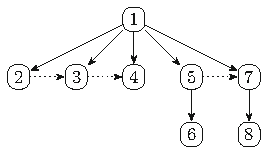
\includegraphics[width=.48\linewidth]{assets/front/dependencies.pdf}
\caption{章节之间的依赖关系. 实线箭头表示先修要求，虚线箭头表示引用关系.}\label{fig:front.1}
\end{figure}

每章最后都有一系列习题，让读者将所学概念用于正文没有讨论的问题.

\subsection*{致谢}\label{sec:acknowledgments}

\noindent\textbf{Sinho Chewi}\quad 最优传输并不是我读研究生时原本计划研究的方向，但它使我的科研生涯变得丰富得多. 为此，我感谢导师兼合作者Philippe，他勇于引领我进入这个美丽的领域；也感谢我的同门兼合作者Jon，他为我开辟道路，并不断给我灵感.

我对最优传输的理解来自许多来源，最初是Villani写作精湛的专著\cite{ref315}，还包括与合作者及Philippe课题组成员数不清的讨论时光. 我很高兴有机会通过这本教学著作为共同体的发展出一份力.

感谢高等研究院提供友好的工作环境，并通过Eric和Wendy Schmidt基金给予支持.

\noindent\textbf{Jonathan Niles-Weed}\quad 我很幸运能向许多才华横溢的合作者学习最优传输；其中，Jason Altschuler、Francis Bach、Sivaraman Balakrishnan、Quentin Berthet、Marco Cuturi、Vincent Divol、Alberto González-Sanz、Tudor Manole、Aram-Alexandre Pooladian、Austin Stromme与Larry Wasserman对我的影响尤其深远. 对他们的知识与见解，我深怀感激. 能在本书中分享他们的一些工作，是我的荣幸.

感谢2021年参加纽约大学研究生讨论班的学生，讨论班涉及本书部分内容，他们的反馈显著改善了表述. 我还要再次感谢Sivaraman Balakrishnan对本书早期版本提出的敏锐意见.

当然，若没有同事兼朋友Sinho Chewi与Philippe Rigollet，就不会有今天的我. 你们给我的启发难以衡量. 与你们合作是我职业生涯最精彩的经历之一，希望今后仍能有幸继续合作.

我在这些讲义上的工作主要由美国国家科学基金会CAREER奖DMS-2339829及其他若干NSF项目（DMS-2015291、DMS-2210583）支持，还得到Sloan基金会研究奖及Apple、Google的资助.

\noindent\textbf{Philippe Rigollet}\quad 自我有幸于2019年在圣弗卢尔开设系列讲座以来，这些讲义已经大幅扩充；最初讲座大致涵盖\autoref{sec:1}、\autoref{sec:7}和\autoref{sec:8}. 初次授课时，本书如今呈现的许多材料对我还很陌生.

首先，我衷心感谢2019年圣弗卢尔暑期学校的组织者，特别是Christophe Bahadoran，以及所有参与者. 听众提供的宝贵反馈，对促成这些讲义主题的大幅扩展起了关键作用. 我唯一的遗憾是成稿迟延，未能与出色的共同讲师Nicolas Curien和Elchanan Mossel的讲义同时出版. 尽管不能合为一卷，我们永远会以Chevaliers du Taste-fourme的身份相联.

我学到的大部分知识来自他人，感谢向我传授了许多这一主题知识的合作者：Jason Altschuler、Julien Clancy、Max Daniels、Aiden Forrow、Borjan Geshkovski、Florian Gunsilius、Jan-Christian Hütter、Cyril Letrouit、Jean-Michel Loubes、Chen Lu、Tyler Maunu、Mor Nitzan、Quentin Paris、Geoff Schiebinger、Austin Stromme、George Stepaniants、Felipe Suarez、William Torous、Kaizheng Wang、Yuling Yan和Aleksandr Zimin. 对于最优传输及其他主题上的启发性讨论，我还要特别感谢Sébastien Bubeck、Ramon van Handel、Thibaut Le Gouic、Vianney Perchet、Yury Polyanskiy、Maxim Raginsky和Justin Solomon. \autoref{sec:5}和\autoref{sec:6}中的许多思想是2021年秋伯克利Simons研究院“优化与抽样中的几何方法”项目的核心讨论话题. 感谢所有参与者、共同组织者及Peter Bartlett，使这一项目如此精彩而富有启发.

此后，统计最优传输共同体显著壮大，这些讲义也从与许多人的交流中受益. 从我们同在普林斯顿时把我引入最优传输的Marco Cuturi开始，我还从Guillaume Carlier、Victor Chernozhukov、Lenaïc Chizat、Simone Di Marino、Augusto Gerolin、Promit Ghosal、Marc Hallin、Zaid Harchaoui、Kengo Kato、Anna Korba、Alexei Kroshnin、Qin Li、Jan Maas、Axel Munk、Robert McCann、Dan Mikulincer、Youssef Marzouk、Soumik Pal、Victor Panaretos、Gabriel Peyré、Filippo Santambrogio、Bodhi Sen、Vladimir Spokoiny、Yair Shenfeld和Jia-Jie Zhu等人那里学到了许多最优传输知识.

部分材料曾于2023和2024年在麻省理工学院、2022年在巴黎索邦大学，以及2023年的两所暑期学校——普林斯顿机器学习理论暑期学校和意大利Cetraro的CIME暑期学校——讲授. 听众给予了出色反馈，促进讲义改进. 特别感谢Théo Dumont、Max Daniels和Giulia Bertagnolli分别录入相关材料.

Michael Diao、Haruki Kono、Hugo Lavenant、Aimee Maurais、Yaroslav Mukhin、Madhav Sankaranarayanan、Sabarish Sainathan、Yucheng Shang、Vishwak Srinivasan、Panos Tsimpos、Oliver Wang、Liane Xu和Julie Zhu纠正了一些排印错误与差错. 感谢他们帮助提高书稿的可读性.

最后，感谢出色的共同作者Sinho Chewi和Jonathan Niles-Weed. 谢谢你们与我一道踏上这场壮阔冒险. 我从你们身上学到的比从任何其他人身上都多；对我而言，你们既是学生，也同样是老师.

我在这些讲义上的工作主要获NSF项目CCF-1838071以及2019--2024年间的其他若干美国国家科学基金会项目（DMS-1712596、CCF-1740751、DMS-2022448、CCF-2106377）支持. 也感谢Apple的资助. 初稿构思于2019年春，当时我在高等研究院获Eric和Wendy Schmidt基金支持.

\noindent\textbf{利益冲突}\quad 作者声明，不存在与本书稿内容相关、需要披露的利益冲突.

\vspace{0.5cm}
\noindent\begin{tabular}{ll}
美国康涅狄格州纽黑文 & Sinho Chewi\\
纽约州纽约 & Jonathan Niles-Weed\\
美国马萨诸塞州剑桥 & Philippe Rigollet
\end{tabular}\par
\noindent 2024年7月

\endgroup
\clearpage\tableofcontents\clearpage
\pagenumbering{arabic}
\section{最优传输}\label{sec:1}
\subsection{最优传输问题}\label{sec:1.1}

Monge 在其 1781 年的论文\cite{ref231}中提出了如下问题：怎样把一堆给定的沙子搬运过去，填满一个给定的沟渠，并使搬运沙子的成本最小？这个问题可以用概率分布建模. 首先注意，要使这项任务能够完成，沙堆与沟渠必须具有相同的体积. 不失一般性，将这个体积归一化为 $1$. 由此，我们需要考虑 $\mathbb R^d$ 上的两个概率测度 $\mu$ 和 $\nu$. 借助两个随机变量 $X\sim\mu$、$Y\sim\nu$ 来思考通常更方便. 它们就是这个约束优化问题的输入.

\subsubsection{Monge 问题与 Kantorovich 问题}\label{sec:1.1.1}

回到搬沙子的类比，搬运沙堆意味着寻找一个称为\emph{传输映射}（transport map）的可测函数 $T:\mathbb R^d\to\mathbb R^d$，它规定位于 $x\in\mathbb R^d$ 的沙子应搬到 $T(x)\in\mathbb R^d$. 要让传输映射真正完成任务，即填满沟渠，就必须保证只要 $X\sim\mu$，便有 $T(X)\sim\nu$. 此时称 $T$ 将 $\mu$ \emph{推前}至 $\nu$，或者称 $\nu$ 是 $\mu$ 经由 $T$ 得到的\emph{推前测度}（pushforward measure），记为 $T_\#\mu=\nu$. 这就是我们的约束.

现在来看目标函数. 回顾 Monge 的问题，我们要使搬运沙子的成本最小. 成本可以用许多方式衡量，例如体力消耗或燃料消耗等. 为简化叙述，这里仅用沙子移动的欧氏距离来衡量. 位于 $x$ 的沙子移动的距离为 $\lVert T(x)-x\rVert$. 因而，平均移动距离为
$$
\int\lVert T(x)-x\rVert\,\mu(dx).
$$
因此，最优传输问题（optimal transport problem）的 Monge 表述\index{Monge problem@Monge问题（Monge problem）|hyperpage}，是在 $T$ 将 $\mu$ 推前至 $\nu$ 的约束下，使上述目标最小化：
$$
\inf_{T:T_\#\mu=\nu}\int\lVert T(x)-x\rVert\,\mu(dx).
$$
注意，传输成本还有许多其他选择. 最一般地，通常考虑一般成本 $c(X,T(X))$，其中 $c(x,y)$ 衡量把 $x\in\mathbb R^d$ 搬到 $y\in\mathbb R^d$ 的成本. 在这一一般框架下，甚至可以允许 $X$ 和 $Y$ 定义在两个不同的空间上，而不必都是 $\mathbb R^d$. 本讲义主要关注 $c(x,y)=\lVert x-T(x)\rVert$ 或 $c(x,y)=\lVert x-T(x)\rVert^2$ 的情形，它们导出 Wasserstein 距离（Wasserstein distance）. 空间 $\mathbb R^d$ 也可以换成更复杂的空间，例如黎曼流形，但这通常超出了本讲义的范围（\autoref{sec:5.6}除外）.

虽然 Monge 问题很容易表述，但仍有几个问题需要回答：
\begin{itemize}
\item 这样的有效传输映射是否总是存在？反过来说，约束集合是否可能为空？
\item 如果存在极小化解，它是否唯一？如何刻画它？注意，我们的约束不是凸的，因此这个问题相当难以回答.
\end{itemize}
一个简单的例子便能回答第一个问题. 取 $d=1$，设 $\mu=\delta_0$ 是位于 $0$ 的点质量，而 $\nu=\frac12\delta_{-1}+\frac12\delta_1$ 是两个点质量的混合. 无论怎样选择传输映射 $T$，推前测度 $T_\#\mu$ 都是位于 $T(0)$ 的点质量 $\delta_{T(0)}$，因此根本无法完成传输，至少确定性映射做不到.

直观地，我们希望有
$$
T(0)=\begin{cases}
-1,&\text{以概率 }\frac12,\\
1,&\text{以概率 }\frac12,
\end{cases}
\qquad\text{且}\qquad
T(x)=x,\quad\forall x\ne0.
$$
这样的 $T$ 不是函数，而是一个 Markov 核（Markov kernel）：它为每个点 $x\in\mathbb R$ 指定一个概率分布.

第二个问题在此后近两个世纪中一直没有令人满意的答案，直到苏联数学家 Leonid Kantorovich 在一篇具有开创性的两页论文\cite{ref173}中引入了该问题的一个松弛形式，恰好允许使用上例所讨论的 Markov 核. 等价地，这种表述涉及的是耦合，而不是映射.

设 $\mu,\nu$ 是 $\mathbb R^d$ 上的两个概率测度，$\gamma$ 是这两个分布的一个\emph{耦合}（coupling），即 $\mathbb R^d\times\mathbb R^d$ 上的一个联合分布，其第一边缘分布为 $\mu$，第二边缘分布为 $\nu$：对于任意 Borel 集 $A\in\mathbb R^d$，有
$$
\gamma(A\times\mathbb R^d)=\mu(A)
\qquad\text{且}\qquad
\gamma(\mathbb R^d\times A)=\nu(A).
$$
之所以使用“耦合”一词，是因为原本 $X\sim\mu$ 与 $Y\sim\nu$ 是互不相关的两个随机变量，而耦合通过描述它们的概率依赖关系，使它们处在同一个概率空间上. 本讲义以下始终用 $\Gamma_{\mu,\nu}$ 表示 $\mu$ 和 $\nu$ 的所有耦合组成的集合.

设 $c:\mathbb R^d\times\mathbb R^d\to[0,\infty)$ 是可测成本函数. 最优传输问题的一般 Kantorovich 表述就是下面的优化问题：
\begin{equation}\tag{KOT}\label{eq:KOT}\index{Kantorovich problem@Kantorovich问题（Kantorovich problem）|hyperpage}
\inf_{\gamma\in\Gamma_{\mu,\nu}}\int c(x,y)\,\gamma(dx,dy).
\end{equation}

\subsubsection{耦合}\label{sec:1.1.2}

为了更好地理解 Kantorovich 问题，考察集合 $\Gamma_{\mu,\nu}$ 很有帮助.

也许最简单的耦合是\emph{独立耦合}（independent coupling）$\gamma=\mu\otimes\nu$，这里仅假设 $X\sim\mu$ 与 $Y\sim\nu$ 相互独立：对于任意 Borel 集 $A,B\subseteq\mathbb R^d$，
$$
\gamma(A\times B)=\mu(A)\cdot\nu(B).
$$
下一个命题汇集了关于 $\Gamma_{\mu,\nu}$ 的一些初步事实.

\begin{proposition}\label{prop:1.1}
设 $\mu,\nu$ 是 $\mathbb R^d$ 上的两个概率测度. 两者的耦合集合 $\Gamma_{\mu,\nu}$ 非空、凸，并且在弱收敛拓扑下是紧的.
\end{proposition}
\begin{proof}
由于独立耦合总是存在，所以 $\Gamma_{\mu,\nu}\ne\varnothing$.

为证明 $\Gamma_{\mu,\nu}$ 是凸的，考虑两个耦合 $\gamma_0,\gamma_1\in\Gamma_{\mu,\nu}$，对任意 $\lambda\in(0,1)$ 定义混合 $\gamma_\lambda=(1-\lambda)\gamma_0+\lambda\gamma_1$. 注意，对于任意 Borel 集 $A\in\mathbb R^d$，
$$
\begin{aligned}
\gamma_\lambda(A\times\mathbb R^d)
&=(1-\lambda)\gamma_0(A\times\mathbb R^d)+\lambda\gamma_1(A\times\mathbb R^d)\\
&=(1-\lambda)\mu(A)+\lambda\mu(A)=\mu(A).
\end{aligned}
$$
因此 $\gamma_\lambda$ 的第一边缘分布为 $\mu$，同理，其第二边缘分布为 $\nu$. 所以任意 $\lambda\in(0,1)$ 都有 $\gamma_\lambda\in\Gamma_{\mu,\nu}$，从而 $\Gamma_{\mu,\nu}$ 是凸的.

为完成这个命题的证明，我们证明 $\Gamma_{\mu,\nu}$ 是紧的. 根据 Prokhorov 定理（\autoref{thm:B.3}），只需证明 $\Gamma_{\mu,\nu}$ 是闭的且（一致）紧的测度族. 为此，回顾 Prokhorov 定理可知，常值序列 $(\mu)_n$、$(\nu)_n$ 都是紧的，因而对任意 $\varepsilon>0$，存在紧集 $K\subset\mathbb R^d$ 使 $\mu(K^c)+\nu(K^c)<\varepsilon$. 于是 $K\times K$ 也是紧集，且对任意 $\gamma\in\Gamma_{\mu,\nu}$，
$$
\begin{aligned}
\gamma\bigl((K\times K)^c\bigr)
&\le\gamma(\mathbb R^d\times K^c)+\gamma(K^c\times\mathbb R^d)\\
&=\mu(K^c)+\nu(K^c)<\varepsilon.
\end{aligned}
$$
因此 $\Gamma_{\mu,\nu}$ 是紧的测度族. 此外，$\gamma\in\Gamma_{\mu,\nu}$ 等价于：对所有有界连续函数 $f:\mathbb R^d\to\mathbb R$，
$$
\int f(x)\,\gamma(dx,dy)=\int f\,d\mu
\qquad\text{且}\qquad
\int f(y)\,\gamma(dx,dy)=\int f\,d\nu.
$$
由弱收敛的定义（\autoref{thm:B.4}）可知 $\Gamma_{\mu,\nu}$ 是闭的. 因此，Prokhorov 定理表明 $\Gamma_{\mu,\nu}$ 是紧的.
\end{proof}

耦合 $\gamma\in\Gamma_{\mu,\nu}$ 刻画两个随机变量 $X\sim\mu$ 与 $Y\sim\nu$ 之间的依赖关系. 如上所述，一种选择是假设 $X$ 与 $Y$ 独立，由此得到独立耦合. 在\autoref{fig:1.1}（左）中，我们绘出了两个高斯混合分布之间的独立耦合. 作为独立耦合的另一个极端，举例来说，设 $X\sim\mathcal N(0,1)$、$Y\sim\chi_1^2$，注意 $Y$ 与 $X^2$ 同分布. 因此可以采用满足 $Y=X^2$ 的\emph{确定性耦合}（deterministic coupling）：
$$
\gamma(dx,dy)=\mu(dx)\,\delta_{x^2}(dy).
$$
我们在\autoref{fig:1.1}（右）中绘出了这个耦合；注意它是退化的.

\begin{figure}[htbp]
\centering
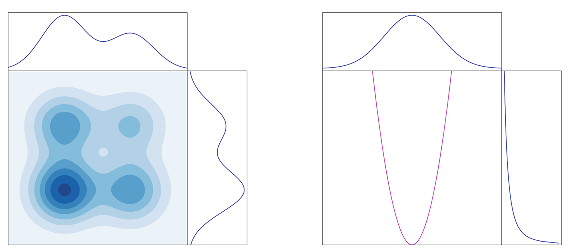
\includegraphics[width=\linewidth]{assets/chapter1/fig1-1.pdf}
\caption{（左）两个高斯分布的混合分布之独立耦合.（右）$X\sim\mathcal N(0,1)$ 与 $Y\sim\chi_1^2$ 的确定性耦合.}\label{fig:1.1}
\end{figure}

\begin{figure}[htbp]
\centering
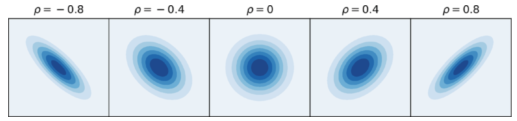
\includegraphics[width=\linewidth]{assets/chapter1/fig1-2.pdf}
\caption{$\rho$ 取五个不同值时，\eqref{eq:1.1} 所示的二元高斯耦合.}\label{fig:1.2}
\end{figure}

继续考察耦合，假设 $X\sim\mathcal N(0,1)$、$Y\sim\mathcal N(0,1)$，则可以采用任意满足下式的耦合：
\begin{equation}\label{eq:1.1}
\begin{pmatrix}X\\Y\end{pmatrix}
\sim\mathcal N\!\left(\begin{pmatrix}0\\0\end{pmatrix},
\begin{pmatrix}1&\rho\\\rho&1\end{pmatrix}\right),
\end{equation}
其中 $\rho\in[-1,1]$ 是 $X$ 与 $Y$ 的相关系数，见\autoref{fig:1.2}.

本章后面的 Brenier 定理表明，在温和的正则条件下，二次成本 Kantorovich 问题的解由一个确定性耦合达到. 正如下文将讨论的，当 $\mu$ 和 $\nu$ 是离散测度时，可以通过考察集合 $\Gamma_{\mu,\nu}$ 的几何来理解这一事实.

\subsubsection{离散最优传输}\label{sec:1.1.3}

$\mu$ 和 $\nu$ 为两个离散分布的情形，在实践中尤其重要. 例如，$\mu,\nu$ 可以是点云上的经验测度. 考虑
$$
\mu=\sum_{i=1}^m p_i\delta_{x_i},
\qquad\text{且}\qquad
\nu=\sum_{j=1}^n q_j\delta_{y_j}.
$$
此时，$X\sim\mu$ 与 $Y\sim\nu$ 的耦合 $\gamma$ 可由非负矩阵 $P\in\mathbb R^{m\times n}$ 刻画，其中 $P_{i,j}=\gamma(X=x_i,Y=y_j)$. $\gamma\in\Gamma_{\mu,\nu}$ 的边缘约束直接转化为
$$
\forall i\in[m],\quad\sum_{j\in[n]}P_{i,j}=p_i,
\qquad\text{且}\qquad
\forall j\in[n],\quad\sum_{i\in[m]}P_{i,j}=q_j.
$$
分别用 $\mathbf1_m$、$\mathbf1_n$ 表示长度为 $m$、$n$ 的全一向量，这些约束就可简洁地表示为 $P\mathbf1_n=p$、$P^{\mathsf T}\mathbf1_m=q$，其中 $p=(p_1,\ldots,p_n)^{\mathsf T}$、$q=(q_1,\ldots,q_m)^{\mathsf T}$.

与耦合类似，成本 $c$ 也可以由一个 $m\times n$ 矩阵 $C$ 表示，其中 $C_{i,j}=c(x_i,y_j)$，$i\in[m]$、$j\in[n]$. 因此 Kantorovich 最优传输问题 \eqref{eq:KOT} 等价于
$$
\min_{P\in\mathbb R_+^{m\times n}}\sum_{i,j\in[n]}C_{i,j}P_{i,j}
\qquad\text{满足}\qquad
P\mathbf1_n=p,\quad P^{\mathsf T}\mathbf1_m=q,
$$
也可以更简洁地写为
$$
\min_{P\in\mathbb R_+^{m\times n}}\langle C,P\rangle
\qquad\text{满足}\qquad
P\mathbf1_n=p,\quad P^{\mathsf T}\mathbf1_m=q,
$$
其中 $\langle C,P\rangle=\operatorname{tr}(C^{\mathsf T}P)$ 是实 $m\times n$ 矩阵空间上的 Frobenius 内积.

特别地，当 $m=n$，并且所有权重 $p_i$、$q_j$ 均为 $1/n$ 时，有效耦合矩阵 $P$ 的集合就是双随机矩阵集合的一个倍数，后者也称为 Birkhoff\index{Birkhoff polytope@Birkhoff多面体（Birkhoff polytope）|hyperpage} 多面体（Birkhoff polytope）：
\begin{equation}\label{eq:1.2}
\operatorname{Birk}:=\{\gamma\in\mathbb R_+^{n\times n}:\gamma\mathbf1_n=\mathbf1_n,\ \mathbf1_n^{\mathsf T}\gamma=\mathbf1_n^{\mathsf T}\}.
\end{equation}
此时，\eqref{eq:KOT} 化为
\begin{equation}\label{eq:1.3}
\min_{P\in n^{-1}\operatorname{Birk}}\langle C,P\rangle.
\end{equation}
Birkhoff 多面体的极点是置换矩阵：它们是二元矩阵 $\pi\in\{0,1\}^{n\times n}$，每行每列恰有一个非零元素. 特别地，根据凸几何的一般原理，形如 \eqref{eq:1.3} 的任意线性规划都可以取一个形如 $n^{-1}\pi$ 的矩阵作为解. 这种形式的传输方案由一个确定性映射（即置换）诱导，因此此时 Monge 问题有解. 正如后续各节将展示的，更一般地，$\Gamma_{\mu,\nu}$ 的极点在最优传输问题的几何中扮演着特殊角色.

\subsection{Wasserstein 距离}\label{sec:1.2}

Kantorovich 问题 \eqref{eq:KOT} 对许多不同的成本函数都有意义，而每种情形都有不同的解释. 例如，一个自然的例子是取平凡度量 $c(x,y)=\mathbbm{1}_{x\ne y}$. 此时 \eqref{eq:KOT} 给出
$$
\inf_{\gamma\in\Gamma_{\mu,\nu}}\gamma(X\ne Y),
$$
这是全变差距离（total variation distance）的一个熟知表述，见\autoref{exer:9}. 然而，注意平凡距离 $\mathbbm{1}_{x\ne y}$ 与 $\mathbb R^d$ 的几何无关. 特别地，它只区分 $x$ 与 $y$ 是否不同，而不说明两者相距多远. 全变差也表现出这一局限. 事实上，若 $\mu=\delta_x$、$\nu=\delta_y$，则只要 $x\ne y$，\eqref{eq:KOT} 的目标值就等于 $1$.

要从 Kantorovich 问题得到一个具有几何意义的量，就必须选择能反映 $x$ 与 $y$ 之间实际距离的成本. 这个想法导出了 Wasserstein 距离. 对任意 $p\ge1$，用 $\mathcal P_p(\mathbb R^d)$ 表示配备欧氏范数 $\lVert\cdot\rVert$ 的 $\mathbb R^d$ 上所有具有有限 $p$ 阶矩的概率测度组成的集合：
$$
\mu\in\mathcal P_p(\mathbb R^d)
\quad\Longleftrightarrow\quad
\int\lVert x\rVert^p\,\mu(dx)<\infty.
$$
两个概率测度 $\mu,\nu\in\mathcal P_p(\mathbb R^d)$ 之间的 $p$-Wasserstein 距离定义为
$$
W_p(\mu,\nu)=\inf_{\gamma\in\Gamma_{\mu,\nu}}
\left(\int\lVert x-y\rVert^p\,\gamma(dx,dy)\right)^{1/p},
$$
其中回顾一下，$\Gamma_{\mu,\nu}$ 是 $\mu$ 与 $\nu$ 的耦合集合.

首先证明，上述下确界实际上能够达到. 为此，定义
$$
I(\gamma):=\int\lVert x-y\rVert^p\,\gamma(dx,dy),
$$
注意根据定义，存在 $\Gamma_{\mu,\nu}$ 中的序列 $(\gamma_n)_n$，使 $I(\gamma_n)\to W_p^p(\mu,\nu)$. 由于 $\Gamma_{\mu,\nu}$ 是紧的（\autoref{prop:1.1}），$(\gamma_n)_n$ 有一个子序列收敛到某个 $\bar\gamma\in\Gamma_{\mu,\nu}$. 根据定义，$W_p(\mu,\nu)\le I(\bar\gamma)$. 由于 $(x,y)\mapsto\lVert x-y\rVert^p$ 无界，$I$ 并不连续，但它是下半连续的，因此 $I(\bar\gamma)\le\liminf_{n\to\infty}I(\gamma_n)=W_p^p(\mu,\nu)$（portmanteau 定理的第三条，\autoref{thm:B.4}）. 从而 $I(\bar\gamma)=W_p^p(\mu,\nu)$. 注意，这个证明中关于成本函数所用的唯一性质就是下半连续性，因此该论证很容易推广到更一般的成本.

由此，可以采用如下 Wasserstein 距离的定义. 注意，这些距离实际上应该称为 Kantorovich--Rubinstein 距离，不过我们仍沿用当下的“Wasserstein 化”潮流.

\begin{definition}\label{def:1.2}\index{Wasserstein distance@Wasserstein距离（Wasserstein distance）|hyperpage}
两个概率测度 $\mu,\nu\in\mathcal P_p(\mathbb R^d)$ 之间的 $p$-Wasserstein 距离定义为
$$
W_p(\mu,\nu)=\min_{\gamma\in\Gamma_{\mu,\nu}}
\left(\int\lVert x-y\rVert^p\,\gamma(dx,dy)\right)^{1/p}.
$$
\end{definition}

\Needspace{8\baselineskip}
\begin{proposition}\label{prop:1.3}
$p$-Wasserstein 距离在 $\mathcal P_p(\mathbb R^d)$ 上定义了一个度量，即对任意 $\mu,\nu\in\mathcal P_p(\mathbb R^d)$：
\begin{enumerate}
\item\label{item:1.3.1} $W_p(\mu,\nu)\ge0$.
\item\label{item:1.3.2} $W_p(\mu,\nu)=W_p(\nu,\mu)$.
\item\label{item:1.3.3} $W_p(\mu,\nu)=0$ 当且仅当 $\mu=\nu$.
\item\label{item:1.3.4} 对任意 $\rho\in\mathcal P_p(\mathbb R^d)$，$W_p(\mu,\nu)\le W_p(\mu,\rho)+W_p(\rho,\nu)$.
\end{enumerate}
\end{proposition}
\begin{proof}
首先注意，\hyperref[item:1.3.1]{第 1 条}和\hyperref[item:1.3.2]{第 2 条}显然成立.

现在证明\hyperref[item:1.3.3]{第 3 条}. 若 $\mu=\nu$，则测度 $\gamma(dx,dy)=\mu(dx)\delta_x(dy)$ 是有效耦合，即 $\gamma\in\Gamma_{\mu,\nu}$. 具体地，$\gamma$ 是 $X\sim\mu$ 时 $(X,X)$ 的分布. 因此
$$
0\le W_p^p(\mu,\mu)\le\int\lVert x-y\rVert^p\,\gamma(dx,dy)
=\int\lVert x-x\rVert^p\,\mu(dx)=0.
$$
为证明\hyperref[item:1.3.3]{第 3 条}的反方向，注意若 $W_p(\mu,\nu)=0$，则存在 $\bar\gamma\in\Gamma_{\mu,\nu}$，使 $(X,Y)\sim\bar\gamma$ 且 $X=Y$ 几乎必然成立；特别地，它们必然同分布，即 $\mu=\nu$.

为完成证明，检验\hyperref[item:1.3.4]{第 4 条}的三角不等式. 为此使用粘合引理（gluing lemma，\autoref{lem:B.5}），它保证存在 $X,Y,Z$，满足 $X\sim\mu$、$Y\sim\nu$、$Z\sim\rho$，并且 $(X,Z)$ 与 $(Z,Y)$ 都是最优耦合. 于是
$$
\begin{aligned}
W_p(\mu,\nu)
&\le\bigl(\mathbb E\lVert X-Y\rVert^p\bigr)^{1/p}\\
&=\bigl(\mathbb E\lVert X-Z+Z-Y\rVert^p\bigr)^{1/p}\\
&\le\bigl(\mathbb E\lVert X-Z\rVert^p\bigr)^{1/p}
+\bigl(\mathbb E\lVert Z-Y\rVert^p\bigr)^{1/p}\\
&=W_p(\mu,\rho)+W_p(\rho,\nu),
\end{aligned}
$$
其中第一行使用了耦合 $(X,Y)$ 的次优性，第三行使用了 $L^p$ 范数的三角不等式，最后一行使用了耦合 $(X,Z)$ 与 $(Z,Y)$ 的最优性.
\end{proof}

\begin{example}[简单情形下的 Wasserstein 距离]\label{ex:1.4}\leavevmode
\begin{enumerate}
\item 固定 $x,y\in\mathbb R^d$，则
$$
W_p(\delta_x,\delta_y)=\lVert x-y\rVert.
$$
因此，$(\mathbb R^d,\lVert\cdot\rVert)$ 通过 $x\mapsto\delta_x$ 等距嵌入 $(\mathcal P_p(\mathbb R^d),W_p)$.
\item 固定 $x,y\in\mathbb R^d$ 及 $0\le\lambda,\tau\le1$，则
$$
W_p\bigl(\lambda\delta_x+(1-\lambda)\delta_y,\tau\delta_x+(1-\tau)\delta_y\bigr)
=|\lambda-\tau|^{1/p}\lVert x-y\rVert.
$$
\end{enumerate}
\end{example}

注意，由 $L^p$ 范数的序关系可知，只要 $p\le q$，就有 $W_p(\mu,\nu)\le W_q(\mu,\nu)$. 特别地，Wasserstein 距离中最小的是 $W_1$.

Wasserstein 距离在随机变量上诱导了一种有用的拓扑：它们使紧空间上的弱收敛度量化；相关背景见\autoref{sec:B}. 更具体地，序列 $(\mu_n)_n$ 满足 $W_p(\mu_n,\mu)\to0$，当且仅当它弱收敛于 $\mu$（记为 $\mu_n\rightsquigarrow\mu$），并且 $p$ 阶矩收敛，即 $\int\lVert\cdot\rVert^p\,d\mu_n\to\int\lVert\cdot\rVert^p\,d\mu$. 这种“度量化”性质可以在最优传输的所有主要教材中找到，也常被用来论证使用 Wasserstein 距离而不是其他距离的合理性. 然而，这几乎算不上一个能将它与其他距离区分开的特征：许多其他距离，例如 L\'evy--Prokhorov 距离、Fortet--Mourier 距离等，也具有这一性质，见\cite[第 6 章]{ref317}. 实际上，这个广为人知的结果并没有充分揭示对于某个 $\varepsilon$，$W_p(\mu,\nu)\le\varepsilon$ 所具有的定量含义.

例如，下面的命题说明，如果两个尾部足够轻的随机变量在任意 $p>1$ 的 $p$-Wasserstein 距离下接近，那么它们的所有矩也一定接近. 我们通过考虑次指数随机变量（sub-exponential random variable），来形式化尾部轻这一假设；这里指满足下式的随机变量 $Z$：
\begin{equation}\label{eq:1.4}
\mathbb E e^{|Z|}\le2.
\end{equation}
对于这样的随机变量，有如下界.

\begin{proposition}\label{prop:1.5}
设 $X\sim\mu$ 和 $Y\sim\nu$ 是两个次指数随机变量. 则对于任意 $p>1$，存在常数 $C_p>0$，使任意整数 $\ell\ge1$ 都满足
$$
\bigl|\mathbb E|X|^\ell-\mathbb E|Y|^\ell\bigr|
\le(C_p\ell)^\ell W_p(\mu,\nu).
$$
\end{proposition}
\begin{proof}
由函数 $x\mapsto|x|^\ell$（$\ell\ge1$）的凸性，
$$
|X|^\ell-|Y|^\ell
\le\ell|X-Y|\bigl(|X|^{\ell-1}\vee|Y|^{\ell-1}\bigr).
$$
对两边取期望，并应用 H\"older 不等式，得到对任意耦合 $(X,Y)$，
$$
\begin{aligned}
\bigl|\mathbb E|X|^\ell-\mathbb E|Y|^\ell\bigr|
&\le\ell\bigl(\mathbb E|X-Y|^p\bigr)^{1/p}
\bigl(\mathbb E(|X|^{\ell-1}\vee|Y|^{\ell-1})^q\bigr)^{1/q},\\
&\hspace{5em}\frac1p+\frac1q=1.
\end{aligned}
$$
取 $X$ 与 $Y$ 的最优耦合，得到
$$
\bigl|\mathbb E|X|^\ell-\mathbb E|Y|^\ell\bigr|
\le\ell W_p(\mu,\nu)
\bigl(\mathbb E(|X|^{\ell-1}\vee|Y|^{\ell-1})^q\bigr)^{1/q}.
$$
最后，回顾次指数随机变量的一个标准性质\cite{ref314}：若 $Z$ 是次指数的，则对所有 $k\ge1$，$\bigl(\mathbb E[|Z|^k]\bigr)^{1/k}\le k$. 因此
$$
\bigl(\mathbb E(|X|^{\ell-1}\vee|Y|^{\ell-1})^q\bigr)^{\frac1{(\ell-1)q}}
\le2(\ell-1)q\le2\frac{\ell p}{p-1}.
$$
\end{proof}

上述结果令人鼓舞：若得到两个测度之间 Wasserstein 距离的界，就能得到它们的矩之间距离的定量界. 不过，相较于其他常用距离或散度，例如全变差或 Kullback--Leibler 散度，Wasserstein 距离也可能往往相当大；关于这些距离的列表、彼此比较及其与统计问题的关系，见\cite[第 2 章]{ref302}.

然而，Wasserstein 距离通常可以由其他常用距离控制. 例如，下面的结果表明，在有界区域上，Wasserstein 距离受全变差距离控制（背景见\autoref{exer:9}）. 此外，它的证明首次展示了如何给出 Wasserstein 距离的界：只需构造一个（次优的）耦合 $\gamma$，使 $\mathbb E_\gamma\lVert X-Y\rVert^p$ 得到适当控制即可.

\begin{theorem}\label{thm:1.6}
设 $\mu,\nu\in\mathcal P_p(\mathbb R^d)$ 是两个分布，其密度分别为 $f$ 和 $g$. 则对任意 $p\ge1$，
$$
W_p^p(\mu,\nu)\le2^{p-1}\inf_{x_0\in\mathbb R^d}
\int\lVert x-x_0\rVert^p|f(x)-g(x)|\,dx.
$$
特别地，若 $\mu$ 和 $\nu$ 的支撑都包含在同一个直径为 $D$ 的球内，则
$$
W_p^p(\mu,\nu)\le D^p d_{\mathrm{TV}}(\mu,\nu),
$$
其中 $d_{\mathrm{TV}}(\mu,\nu)$ 是 $\mu$ 与 $\nu$ 之间的全变差距离，定义为
$$
d_{\mathrm{TV}}(\mu,\nu)=\frac12\int|f(x)-g(x)|\,dx.
$$
\end{theorem}
\begin{proof}
假设 $\mu\ne\nu$，否则结论显然成立. 正如定理陈述前所提到的，我们将构造 $\mu$ 与 $\nu$ 的一个显式耦合. 为此，考虑三个正函数 $(f-g)_+$、$(f-g)_-$ 与 $f\wedge g$（参见\autoref{fig:1.3}），并注意
$$
\int\bigl((f-g)_+-(f-g)_-\bigr)=\int f-\int g=1-1=0,
$$
\begin{figure}[htbp]
\centering
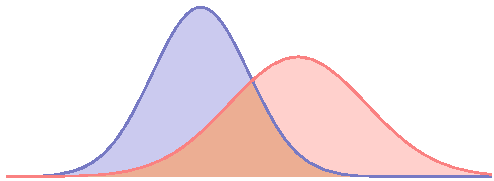
\includegraphics[width=\linewidth]{assets/chapter1/fig1-3.pdf}
\caption{积分 $\int(f-g)_+$、$\int(f-g)_-$ 与 $\int f\wedge g$ 分别对应蓝色、红色与橙色区域.}\label{fig:1.3}
\end{figure}

因此
$$
\int(f-g)_+=\int(f-g)_-=:t>0,
$$
并且
$$
\int f\wedge g
=\frac12\left(\int f+\int g-\int(f-g)_+-\int(f-g)_-\right)=1-t.
$$

接着，将这些函数归一化，得到三个密度
$$
h_+=\frac1t(f-g)_+,\qquad h_-=\frac1t(f-g)_-,\qquad
h_\wedge=\frac1{1-t}f\wedge g.
$$
可以将 $f$ 与 $g$ 重新写成上述密度的混合：
$$
f=th_++(1-t)h_\wedge,\qquad g=th_-+(1-t)h_\wedge.
$$
再令 $Z_+$、$Z_-$、$Z_\wedge$ 是三个相互独立的随机变量，其密度分别为 $h_+$、$h_-$、$h_\wedge$；令 $B$ 是参数为 $t\in(0,1]$ 的 Bernoulli 随机变量，且与 $Z_+$、$Z_-$、$Z_\wedge$ 独立.

现在可以定义 $\mu$ 与 $\nu$ 的耦合了. 为此，令随机变量对 $(X,Y)$ 满足
$$
\begin{aligned}
X&=BZ_++(1-B)Z_\wedge,\\
Y&=BZ_-+(1-B)Z_\wedge,
\end{aligned}
$$
注意 $(X,Y)$ 的分布 $\gamma$ 确实是 $\mu$ 与 $\nu$ 的有效耦合. 结合这一事实与不等式 $\lVert x-y\rVert^p\le2^{p-1}\bigl(\lVert x-x_0\rVert^p+\lVert y-x_0\rVert^p\bigr)$，得到
$$
\begin{aligned}
W_p^p(\mu,\nu)
&\le\mathbb E_\gamma\lVert X-Y\rVert^p\\
&=\mathbb P(B=0)\cdot0
+\mathbb P(B=1)\int\lVert x-y\rVert^p h_+(x)h_-(y)\,dx\,dy\\
&\le t2^{p-1}\left(\int\lVert x-x_0\rVert^p h_+(x)\,dx
+\int\lVert y-x_0\rVert^p h_-(y)\,dy\right)\\
&=t2^{p-1}\left(\int\lVert x-x_0\rVert^p\bigl(h_+(x)+h_-(x)\bigr)\,dx\right)\\
&=2^{p-1}\left(\int\lVert x-x_0\rVert^p\bigl((f-g)_+(x)+(f-g)_-(x)\bigr)\,dx\right)\\
&=2^{p-1}\left(\int\lVert x-x_0\rVert^p|f(x)-g(x)|\,dx\right).
\end{aligned}
$$
再对右端关于 $x_0$ 取最小值，即得结论. 第二个结论只需取 $x_0$ 为上述球的球心，便容易得到.
\end{proof}

$\mu$ 和 $\nu$ 绝对连续的假设是多余的；只要直接操作测度而不是密度，完全相同的证明仍然适用，只是记号会稍显晦涩；见\cite[定理 6.15]{ref317}.

\subsection{一维最优传输}\label{sec:1.3}

为了对最优传输获得一些直观认识，我们考察一个较简单的情形：$\mu$ 和 $\nu$ 是实数轴上的概率测度.在这种情形下，可以定义它们各自的累积分布函数.

回顾一下，随机变量 $Z$ 的\emph{累积分布函数}（cumulative distribution function，CDF）是函数 $F:\mathbb R\to[0,1]$，其定义为
$$
F(t):=\mathbb P(Z\le t),\qquad t\in\mathbb R.
$$
由于 $F$ 单调不减，可以定义其\emph{伪逆}（pseudo-inverse）$F^\dagger$：
$$
F^\dagger(u)=\inf\{t\in\mathbb R:F(t)\ge u\},\qquad u\in[0,1],
$$
其中约定 $\inf\varnothing=\infty$.虽然 $F^\dagger$ 并非真正的逆函数，但它确实满足下述性质：
\begin{equation}\label{eq:1.5}
F^\dagger(u)\le t\quad\Longleftrightarrow\quad u\le F(t).
\end{equation}

这一性质常用于模拟随机变量.设 $U\sim\operatorname{Unif}([0,1])$ 是均匀随机变量，则 $Z\sim F^\dagger(U)$ 的累积分布函数为 $F$.事实上，对任意 $t\in\mathbb R$，
\begin{equation}\label{eq:1.6}
\mathbb P(Z\le t)=\mathbb P(F^\dagger(U)\le t)
=\mathbb P(U\le F(t))=F(t).
\end{equation}

下面的定理利用累积分布函数刻画一维最优传输.

\begin{theorem}\label{thm:1.7}
设 $\mu,\nu\in\mathcal P_1(\mathbb R)$ 是两个概率分布，其累积分布函数分别为 $F_\mu$ 和 $F_\nu$.设 $U\sim\operatorname{Unif}([0,1])$ 是均匀随机变量，以 $\bar\gamma$ 表示 $(F_\mu^\dagger(U),F_\nu^\dagger(U))$ 的分布.那么 $\bar\gamma\in\Gamma_{\mu,\nu}$ 是 $\mu$ 与 $\nu$ 的一个有效耦合，并且它是最优的：
$$
W_1(\mu,\nu)=\int|x-y|\,\bar\gamma(\mathrm dx,\mathrm dy)
=\min_{\gamma\in\Gamma_{\mu,\nu}}\int|x-y|\,\gamma(\mathrm dx,\mathrm dy).
$$
此外，
$$
W_1(\mu,\nu)=\int_{-\infty}^{\infty}|F_\mu(t)-F_\nu(t)|\,\mathrm dt.
$$
\end{theorem}

\begin{proof}
由 \eqref{eq:1.6} 可知 $\bar\gamma\in\Gamma_{\mu,\nu}$，只需再验证其最优性.为此，注意到对任意 $\gamma\in\Gamma_{\mu,\nu}$，若 $(X,Y)\sim\gamma$，则由 Fubini 定理可得
$$
\begin{aligned}
&\int|x-y|\,\gamma(\mathrm dx,\mathrm dy)\\
&\quad=\iint_{-\infty}^{\infty}
  (\mathbbm{1}_{x\le t<y}+\mathbbm{1}_{y\le t<x})\,\mathrm dt\,\gamma(\mathrm dx,\mathrm dy)\\
&\quad=\int_{-\infty}^{\infty}
  \bigl(\gamma(X\le t<Y)+\gamma(Y\le t<X)\bigr)\,\mathrm dt\\
&\quad=\int_{-\infty}^{\infty}
  \bigl(\gamma(X\le t)+\gamma(Y\le t)-2\gamma(X\le t,Y\le t)\bigr)\,\mathrm dt\\
&\quad\ge\int_{-\infty}^{\infty}
  \bigl(F_\mu(t)+F_\nu(t)-2(F_\mu(t)\wedge F_\nu(t))\bigr)\,\mathrm dt\\
&\quad=\int_{-\infty}^{\infty}|F_\mu(t)-F_\nu(t)|\,\mathrm dt.
\end{aligned}
$$
为了说明当 $\gamma=\bar\gamma$ 时，上述不等式成为等式，注意到
$$
\begin{aligned}
\bar\gamma(X\le t,Y\le t)
&=\mathbb P(F_\mu^\dagger(U)\le t,F_\nu^\dagger(U)\le t)\\
&=\mathbb P(U\le F_\mu(t),U\le F_\nu(t))\\
&=\mathbb P(U\le F_\mu(t)\wedge F_\nu(t))\\
&=F_\mu(t)\wedge F_\nu(t).
\end{aligned}
$$
我们已经证明
$$
\int|x-y|\,\gamma(\mathrm dx,\mathrm dy)
\ge\int_{-\infty}^{\infty}|F_\mu(t)-F_\nu(t)|\,\mathrm dt
=\int|x-y|\,\bar\gamma(\mathrm dx,\mathrm dy),
$$
因而 $\bar\gamma$ 是最优耦合.
\end{proof}

如果 $Z$ 存在密度，那么它的累积分布函数 $F$ 实际上是 $F^\dagger$ 的左逆，即 $F\circ F^\dagger=\mathrm{Id}$.如果 $\mu$ 存在密度，这一事实意味着最优耦合 $\bar\gamma$ 具有下述特殊形式：若 $X\sim\mu$，则
\begin{equation}\label{eq:1.7}
(X,F_\nu^\dagger\circ F_\mu(X))\sim\bar\gamma.
\end{equation}
换言之，Monge 问题与 Kantorovich 问题的解相同，因为我们找到了一个传输映射 $\bar T=F_\nu^{-1}\circ F_\mu$，使得 $\bar T_\#\mu=\nu$，并且
$$
\begin{aligned}
\int|x-\bar T(x)|\,\mu(\mathrm dx)
&=\min_{\gamma\in\Gamma_{\mu,\nu}}\int|x-y|\,\gamma(\mathrm dx,\mathrm dy)\\
&=\min_{T:T_\#\mu=\nu}\int|x-T(x)|\,\mu(\mathrm dx).
\end{aligned}
$$

虽然本节着重讨论 $W_1$ 距离，但 \eqref{eq:1.7} 给出的耦合 $\bar\gamma$ 实际上具有普遍最优性：对于任意严格凸成本的 Kantorovich 问题，它都是最优的；这里的严格凸成本指形如 $c(x,y)=h(x-y)$ 的成本，其中 $h:\mathbb R\to\mathbb R$ 严格凸.这包括所有 $p>1$ 的 $W_p$ 距离.参见\autoref{exer:8}.

注意，$\bar T$ 是两个递增函数的复合，因此也是\emph{单调递增}函数.一维的连续单调递增函数是凸函数的导数，这提示我们，可以通过考虑凸函数的梯度，将这一性质推广到高维.高维中这种单调传输映射的存在性，正是 Brenier 的重要结果~\cite{ref55} 的内容.下面我们就来研究这一结果.

\subsection{Brenier 定理}\label{sec:1.4}

对任意 $p\ge1$，$p$-Wasserstein 距离都是一个自然的研究对象.不过，$p=1,2$ 两种情形具有突出的特殊结构，后文的大部分讨论将围绕它们展开.我们先研究 $p=2$ 的情形；这一情形尤为显著的一点，是它与凸分析的密切联系.

回顾一下，
\begin{equation}\tag{$W_2^2$}\label{eq:W22}
W_2^2(\mu,\nu)=\min_{\gamma\in\Gamma_{\mu,\nu}}
\int\|x-y\|^2\,\gamma(\mathrm dx,\mathrm dy).
\end{equation}

\begin{theorem}[Brenier]\label{thm:1.8}\index{Brenier’s theorem@Brenier定理（Brenier’s theorem）|hyperpage}
设 $\mu,\nu\in\mathcal P_2(\mathbb R^d)$ 是两个概率测度，$\mu$ 存在密度，并设 $X\sim\mu$.如果 $\bar\gamma$ 是 \eqref{eq:W22} 的一个最优耦合，即
$$
\int\|x-y\|^2\,\bar\gamma(\mathrm dx,\mathrm dy)
=\min_{\gamma\in\Gamma_{\mu,\nu}}\int\|x-y\|^2\,\gamma(\mathrm dx,\mathrm dy)
=W_2^2(\mu,\nu),
$$
那么存在凸函数 $\varphi:\mathbb R^d\to\mathbb R$，使得 $(X,\nabla\varphi(X))\sim\bar\gamma\in\Gamma_{\mu,\nu}$.
\end{theorem}

Brenier 定理的关键假设是 $\mu$ 存在密度，即 $\mu$ 关于 Lebesgue 测度绝对连续.特别地，由于凸函数在 Lebesgue 几乎处处可微，这一假设保证了 $\nabla\varphi(X)$ 是有意义的.

在开始证明之前，我们先考虑 Brenier 定理在统计学上的一个推论.Brenier 定理断言，只要 $\mu$ 存在密度，那么对任意 $\nu\in\mathcal P_2(\mathbb R^d)$，都存在凸函数 $\phi$，使得 $\nabla\phi_\#\mu=\nu$.由于凸函数的梯度是单调函数在高维的自然对应物，因此该定理大幅推广了\autoref{sec:1.3} 提到的经典一维事实：若 $U\sim\operatorname{Unif}([0,1])$，则 $F_\nu^\dagger(U)\sim\nu$.

在一维情形中，函数 $F_\nu^\dagger$ 称为 $\nu$ 的\emph{分位数函数}（quantile function），在统计学中具有基础性意义.因此，可以利用 Brenier 定理定义多元分位数的概念~\cite{ref75,ref160}.事实证明，这一观点成果丰硕，并催生了广泛的统计应用~\cite{ref159}.（更多细节见\autoref{sec:1.7}.）

回到 Brenier 定理本身，目前还看不出最优传输为何会与凸函数的梯度相关.因此，我们先研究这类梯度，以建立直观认识.

\subsubsection{凸函数的梯度}\label{sec:1.4.1}

首先注意，对连续函数 $f:\mathbb R\to\mathbb R$，存在某个可微凸函数 $\varphi$ 使得 $f=\varphi'$，当且仅当 $f$ 单调不减.事实上，$\varphi$ 的凸性意味着，对任意 $x,y\in\mathbb R$，
\begin{equation}\label{eq:1.8}
\varphi(x)-\varphi(y)\le(x-y)\varphi'(x),
\end{equation}
\begin{equation}\label{eq:1.9}
\varphi(y)-\varphi(x)\le(y-x)\varphi'(y).
\end{equation}
将上述两个不等式相加，得到
$$
(x-y)(\varphi'(x)-\varphi'(y))\ge0,
$$
所以 $\varphi'$ 单调不减.

对于 $\mathbb R^d$ 上的函数，这一结论是否有对应的推广？当然，我们立即得到，对任意 $x,y\in\mathbb R^d$，
$$
\langle x-y,\widetilde\nabla\varphi(x)-\widetilde\nabla\varphi(y)\rangle\ge0,
$$
其中 $\widetilde\nabla\varphi(x)\in\partial\varphi(x)$ 表示 $\varphi$ 在 $x$ 处的一个\emph{次梯度}（subgradient；凸分析的预备知识见\autoref{sec:A}）.遗憾的是，虽然在一维情形中，两点不等式 \eqref{eq:1.8} 和 \eqref{eq:1.9} 能够推出任意点配置所对应的不等式，但在高维中不再如此，因此我们需要刻画更多信息.

实际上，凸性还蕴含许多这样的不等式：任取整数 $k\ge2$ 以及一组点 $x_1,\allowbreak\ldots,\allowbreak x_k\in\mathbb R^d$，有
$$
\begin{aligned}
\varphi(x_i)-\varphi(x_{i+1})
&\le\langle x_i-x_{i+1},\widetilde\nabla\varphi(x_i)\rangle,
&&i=1,\ldots,k-1,\\
\varphi(x_k)-\varphi(x_1)
&\le\langle x_k-x_1,\widetilde\nabla\varphi(x_k)\rangle.
\end{aligned}
$$
将这些不等式相加，得到
\begin{equation}\label{eq:1.10}
\sum_{i=1}^k\langle x_i-x_{i+1},\widetilde\nabla\varphi(x_i)\rangle\ge0,
\end{equation}
其中约定 $x_{k+1}=x_1$.\footnote{采用这一约定后，点 $x_1\to x_2\to\cdots\to x_k\to x_1$ 形成一个“循环”.}

\subsubsection{循环单调性}\label{sec:1.4.2}

由于 $\varphi$ 在 $x$ 处的次微分中可能含有多个点，在将 $\widetilde\nabla\varphi(\cdot)$ 视为从 $\mathbb R^d$ 到 $\mathbb R^d$ 的映射之前，我们先描述其图像 $\{(x,\widetilde\nabla\varphi(x)):x\in\mathbb R^d\}$.首先定义这类图像的一个重要性质.

\begin{definition}\label{def:1.9}\index{cyclical monotonicity@循环单调性（cyclical monotonicity）|hyperpage}
若集合 $A\subset\mathbb R^d\times\mathbb R^d$ 满足：对任意整数 $k\ge2$ 和任意点 $(x_i,y_i)\in A$，$i=1,\ldots,k$，有
\begin{equation}\label{eq:1.11}
\sum_{i=1}^k\langle x_i-x_{i+1},y_i\rangle\ge0,
\end{equation}
其中约定 $x_{k+1}=x_1$，则称 $A$ 是\emph{循环单调的}（cyclically monotone）.
\end{definition}

由 \eqref{eq:1.10} 可知，只要 $\varphi$ 是凸的，集合 $\partial\varphi\subset\mathbb R^d\times\mathbb R^d$ 就是循环单调的.事实上，$\mathbb R^d\times\mathbb R^d$ 的所有循环单调子集都具有这一形式.

\begin{theorem}[Rockafellar]\label{thm:1.10}\index{Rockafellar’s theorem@Rockafellar定理（Rockafellar’s theorem）|hyperpage}
集合 $A\subset\mathbb R^d\times\mathbb R^d$ 是循环单调的，当且仅当存在闭凸函数 $\varphi:\mathbb R^d\to\mathbb R\cup\{\infty\}$，使得
$$
A\subseteq\partial\varphi.
$$
\end{theorem}

这一凸分析经典定理的证明见\autoref{sec:A}.

注意，条件 \eqref{eq:1.11} 等价于要求：对任意点 $(x_i,y_i)\in A$，$i=1,\ldots,k$，有
\begin{equation}\label{eq:1.12}
\sum_{i=1}^k\|x_i-y_i\|^2\le\sum_{i=1}^k\|x_{i+1}-y_i\|^2.
\end{equation}
这一表述使我们能够看出它与最优传输的联系.事实上，为了说明这一点，我们考虑下面的例子.设
$$
\mu=\frac1n\sum_{j=1}^n\delta_{a_j},\qquad
\nu=\frac1n\sum_{j=1}^n\delta_{b_j}.
$$

在这一离散情形中，$\mu$ 与 $\nu$ 之间的全体耦合构成的集合可以与 Birkhoff 多面体等同起来（见\autoref{sec:1.1.3}），其极点是经缩放的置换矩阵.由于离散最优传输问题是一个线性规划，因而可在极点中取到解.因此，我们只需考虑由置换给出的耦合.具体而言，$\{1,\ldots,n\}$ 的一个置换 $\sigma$ 对应于耦合
$$
\gamma=\frac1n\sum_{j=1}^n\delta_{(a_j,b_{\sigma(j)})}.
$$
如果这样的耦合在所有置换中具有最小成本，即
\begin{equation}\label{eq:1.13}
\sum_{j=1}^n\|a_j-b_{\sigma(j)}\|^2
\le\sum_{j=1}^n\|a_j-b_{\tau(j)}\|^2,\qquad\forall\tau,
\end{equation}
那么它就是最优耦合.

这一条件恰好等价于 $\gamma$ 的支集具有循环单调性.事实上，对 $\nu$ 的原子重新编号后，不妨假设 $\sigma$ 为恒等置换.于是，$\gamma$ 的支集由点对 $(a_j,b_j)$，$j\in\{1,\ldots,n\}$，组成.给定任意由 $k$ 个不同点组成的子集 $(x_i,y_i)=(a_{j_i},b_{j_i})\in\operatorname{supp}(\gamma)$，$i=1,\ldots,k$，令 $\tau$ 为 $\{j_1,\ldots,j_k\}$ 上的循环置换，并保持其他指标不变：
$$
\tau(j)=\begin{cases}
j_{i-1},&\text{若 }j=j_i,\ i\in\{2,\ldots,k\},\\
j_k,&\text{若 }j=j_1,\\
j,&\text{其他情形.}
\end{cases}
$$
那么 \eqref{eq:1.13} 就蕴含 \eqref{eq:1.12}.事实上，由于任意置换 $\tau$ 都可以分解为循环，类似的推理也表明，\eqref{eq:1.12} 是 \eqref{eq:1.13} 成立的充分条件.

前面的讨论说明，在离散情形中，最优耦合的支集是循环单调的.在一般情形中也有类似的现象；不过，当 $\gamma$ 不给其支集中的点赋予正质量时，上述论证就不成立了.尽管如此，下面的结果表明，通过对小邻域（例如球）而非单个点进行推理，类似的策略仍可奏效.我们需要小心处理，以保证能够在这些邻域上修改 $\gamma$，同时保持约束 $\gamma\in\Gamma_{\mu,\nu}$.

\begin{proposition}\label{prop:1.11}
设 $\bar\gamma\in\Gamma_{\mu,\nu}$ 是 $\mu$ 与 $\nu$ 之间的最优耦合，即
$$
\int\|x-y\|^2\,\bar\gamma(\mathrm dx,\mathrm dy)
=\min_{\gamma\in\Gamma_{\mu,\nu}}\int\|x-y\|^2\,\gamma(\mathrm dx,\mathrm dy)
=W_2^2(\mu,\nu).
$$
那么 $\operatorname{supp}(\bar\gamma)$ 是循环单调的.
\end{proposition}

\begin{proof}
假设 $S:=\operatorname{supp}(\bar\gamma)$ 不是循环单调的.那么存在 $k\ge2$ 和 $(x_i,y_i)\in S$，$i=1,\ldots,k$，使得
$$
\sum_{i=1}^k\|x_i-y_i\|^2>\sum_{i=1}^k\|x_{i+1}-y_i\|^2.
$$
由欧几里得范数的连续性，对 $i=1,\ldots,k$，分别存在 $x_i,y_i$ 的邻域 $U_i,V_i$，使得 $\bar\gamma(U_i\times V_i)>0$，并且对所有 $\tilde x_i,\tilde x_i'\in U_i$、$\tilde y_i,\tilde y_i'\in V_i$，$i=1,\ldots,k$，均有
\begin{equation}\label{eq:1.14}
\sum_{i=1}^k\|\tilde x_i-\tilde y_i\|^2
>\sum_{i=1}^k\|\tilde x_{i+1}'-\tilde y_i'\|^2.
\end{equation}

现在令 $\gamma_i$，$i=1,\ldots,k$，为 $\mathbb R^d\times\mathbb R^d$ 上的一族（条件）概率分布，定义为：对任意 Borel 集 $A\subset\mathbb R^d\times\mathbb R^d$，有 $\gamma_i(A)=\bar\gamma(A\mid U_i\times V_i)$.接着，以 $\gamma_i^{(1)}$ 和 $\gamma_i^{(2)}$ 分别表示 $\gamma_i$ 的第一和第二边缘分布，并定义混合：
$$
\gamma=\bar\gamma+\frac ck\sum_{i=1}^k
\bigl(\gamma_{i+1}^{(1)}\otimes\gamma_i^{(2)}-\gamma_i\bigr),
$$
其中 $c>0$ 稍后选定，并约定 $\gamma_{k+1}=\gamma_1$.

注意，对任意 Borel 集 $A\subset\mathbb R^d\times\mathbb R^d$，
$$
\begin{aligned}
\gamma(A)&\ge\bar\gamma(A)-\frac ck\sum_{i=1}^k\gamma_i(A)\\
&=\bar\gamma(A)-\frac ck\sum_{i=1}^k\bar\gamma(A\mid U_i\times V_i)\\
&=\bar\gamma(A)-\frac ck\sum_{i=1}^k
\frac{\bar\gamma(A\cap(U_i\times V_i))}{\bar\gamma(U_i\times V_i)}\\
&\ge\bar\gamma(A)-\frac{c\bar\gamma(A)}k\sum_{i=1}^k
\frac1{\bar\gamma(U_i\times V_i)}.
\end{aligned}
$$
所以，只要 $c<\min_{i\in[k]}\bar\gamma(U_i\times V_i)$，就有 $\gamma(A)\ge0$.此外，$\gamma(\mathbb R^d\times\mathbb R^d)=1$，因此 $\gamma$ 的确是 $\mathbb R^d\times\mathbb R^d$ 上的概率分布.

为了验证 $\gamma\in\Gamma_{\mu,\nu}$，注意到对任意 Borel 集 $B\subset\mathbb R^d$，
$$
\begin{aligned}
\gamma(B\times\mathbb R^d)
&=\mu(B)+\frac ck\sum_{i=1}^k
  \bigl(\gamma_{i+1}^{(1)}(B)-\gamma_i(B\times\mathbb R^d)\bigr)\\
&=\mu(B)+\frac ck\sum_{i=1}^k
  \bigl(\gamma_{i+1}^{(1)}(B)-\gamma_i^{(1)}(B)\bigr)\\
&=\mu(B)+\frac ck\bigl(\gamma_{k+1}^{(1)}(B)-\gamma_1^{(1)}(B)\bigr)
=\mu(B).
\end{aligned}
$$
同理，
$$
\begin{aligned}
\gamma(\mathbb R^d\times B)
&=\nu(B)+\frac ck\sum_{i=1}^k
  \bigl(\gamma_i^{(2)}(B)-\gamma_i(\mathbb R^d\times B)\bigr)\\
&=\nu(B)+\frac ck\sum_{i=1}^k
  \bigl(\gamma_i^{(2)}(B)-\gamma_i^{(2)}(B)\bigr)=\nu(B).
\end{aligned}
$$
接着注意到，由 \eqref{eq:1.14}，
$$
\begin{aligned}
&\int\|x-y\|^2\,\gamma(\mathrm dx,\mathrm dy)
-\int\|x-y\|^2\,\bar\gamma(\mathrm dx,\mathrm dy)\\
&\quad=\frac ck\sum_{i=1}^k\left(
\begin{aligned}
&\int_{U_{i+1}\times V_i}\|x-y\|^2\,
\gamma_{i+1}^{(1)}(\mathrm dx)\,\gamma_i^{(2)}(\mathrm dy)\\
&\qquad-\int_{U_i\times V_i}\|x-y\|^2\,\gamma_i(\mathrm dx,\mathrm dy)
\end{aligned}\right)\\
&\quad<0.
\end{aligned}
$$
这与 $\bar\gamma$ 的最优性矛盾.
\end{proof}

\subsubsection{Brenier 定理的证明}\label{sec:1.4.3}

现在我们可以证明 Brenier 定理了.

\begin{proof}[\autoref{thm:1.8}的证明]

设 $\bar\gamma$ 是一个最优耦合.由\autoref{prop:1.11}，$\operatorname{supp}(\bar\gamma)$ 是循环单调的.由 Rockafellar 的\autoref{thm:1.10}，可知存在凸函数 $\varphi:\mathbb R^d\to\mathbb R\cup\{\infty\}$，使得 $\bar\gamma(Y\in\partial\varphi(X))=1$.但是，由于 $\varphi$ 是凸函数，它在定义域的内部局部 Lipschitz 连续，而定义域的边界由凸性可知是零测集.因此，由 Rademacher 定理，$\varphi$ 在其定义域上关于 Lebesgue 测度几乎处处可微.由于 $\mu$ 存在密度，这意味着 $\varphi$ 在 $\mu$ 几乎处处可微.因此，$\bar\gamma(Y=\nabla\varphi(X))=1$，或者换言之，若 $X\sim\mu$，则 $(X,\nabla\varphi(X))\sim\bar\gamma$.
\end{proof}

\subsection{Kantorovich 对偶}\label{sec:1.5}

Brenier 定理表明，若 $\mu$ 有密度，则问题 \eqref{eq:W22} 的最优耦合是由某个凸函数 $\varphi$ 的梯度给出的确定性耦合. 这一结果引出了如下问题：能否通过求解一个优化问题来直接找到 $\varphi$，或者能否验证某个凸函数 $\varphi$ 对应于一个最优耦合？利用凸对偶（convex duality）的工具可以回答这些问题.

在完全离散的情形（见\autoref{sec:1.1.3}），\eqref{eq:W22} 是一个线性规划（linear program，LP），即目标函数和约束均为线性的；线性规划具有实用的对偶理论. 这一直觉也适用于一般情形，而且可以通过逼近论证使二者的联系严格化，见\cite[第 11 章]{ref123}. 事实上，Kantorovich 正是通过最优传输引入了线性规划对偶；自其诞生以来，这一理论一直在推动算法的发展.

\subsubsection{Kantorovich 对偶问题}\label{sec:1.5.1}

\eqref{eq:W22} 的对偶问题是一个最大化问题. 为了求出它的表达式，将约束 $\gamma\in\Gamma_{\mu,\nu}$ 编码为
$$
\begin{aligned}
&\sup_{f,g\in C_b}\left\{
\int f(x)\,\mu(dx)+\int g(y)\,\nu(dy)
-\int\bigl(f(x)+g(y)\bigr)\,\gamma(dx,dy)\right\}\\
&\qquad=\begin{cases}
0,&\text{若 }\gamma\in\Gamma_{\mu,\nu},\\
\infty,&\text{其他情形},
\end{cases}
\end{aligned}
$$
其中上确界取遍 $\mathbb{R}^d$ 上所有连续有界函数组成的集合 $C_b$. 因而，\eqref{eq:W22} 等价于
$$
\begin{aligned}
\inf_{\gamma\in\mathcal{M}_+}\Biggl\{
&\int\|x-y\|^2\,\gamma(dx,dy)\\
&+\sup_{f,g\in C_b}\left\{
\int f(x)\,\mu(dx)+\int g(y)\,\nu(dy)
-\int\bigl(f(x)+g(y)\bigr)\,\gamma(dx,dy)\right\}\Biggr\},
\end{aligned}
$$
其中下确界取遍 $\mathbb{R}^d\times\mathbb{R}^d$ 上所有正测度组成的集合 $\mathcal{M}_+$，不再施加其他限制. 注意，当 $\gamma\notin\Gamma_{\mu,\nu}$ 时，这个新目标函数为无穷大，因此两个问题严格等价.

接下来交换 $\inf$ 与 $\sup$，得到 \eqref{eq:W22} 的最优值的如下下界：
\begin{equation}\label{eq:1.15}
\begin{aligned}
\sup_{f,g\in C_b}\Biggl\{
&\int f(x)\,\mu(dx)+\int g(y)\,\nu(dy)\\
&+\inf_{\gamma\in\mathcal{M}_+}\left\{
\int\bigl(\|x-y\|^2-f(x)-g(y)\bigr)\,\gamma(dx,dy)
\right\}\Biggr\}.
\end{aligned}
\end{equation}

现在注意到，由于 $\gamma$ 是正测度，
$$
\begin{aligned}
&\inf_{\gamma\in\mathcal{M}_+}\left\{
\int\bigl(\|x-y\|^2-f(x)-g(y)\bigr)\,\gamma(dx,dy)\right\}\\
&\qquad=\begin{cases}
0,&\text{若 }f(x)+g(y)\leq\|x-y\|^2,\quad\forall x,y\in\mathbb{R}^d,\\
-\infty,&\text{其他情形}.
\end{cases}
\end{aligned}
$$
的确，若存在一对 $(x,y)$ 违反上述约束，则可以取测度序列 $\gamma_n=n\delta_{(x,y)}$，使该积分趋于 $-\infty$.

因此，我们已经证明 \eqref{eq:W22} 的一个下界为
$$
\sup_{\substack{f,g\in C_b\\f(x)+g(y)\leq\|x-y\|^2}}
\left\{\int f\,d\mu+\int g(y)\,d\nu\right\}.
$$

虽然上面选择 $f,g\in C_b$ 是考虑到概率测度集合上的弱拓扑，但只要一对可积函数 $(f,g)$ 几乎处处满足 $f(x)+g(y)\leq\|x-y\|^2$，它们就给出 $W_2^2(\mu,\nu)$ 的这个下界.

\begin{lemma}\label{lem:1.12}
设 $\mu,\nu\in\mathcal{P}_2(\mathbb{R}^d)$，则
$$
\begin{aligned}
W_2^2(\mu,\nu)
&=\inf_{\gamma\in\Gamma_{\mu,\nu}}\int\|x-y\|^2\,\gamma(dx,dy)\\
&\geq\sup_{\substack{f\in L^1(\mu),\ g\in L^1(\nu)\\
f(x)+g(y)\leq\|x-y\|^2}}
\left\{\int f\,d\mu+\int g\,d\nu\right\}.
\end{aligned}
$$
\end{lemma}
\begin{proof}
设 $f\in L^1(\mu)$、$g\in L^1(\nu)$，使得对 $\mu$ 几乎处处的 $x$、$\nu$ 几乎处处的 $y$，有 $f(x)+g(y)\leq\|x-y\|^2$，并固定 $\gamma\in\Gamma_{\mu,\nu}$. 那么
$$
\begin{aligned}
\int f(x)\,\mu(dx)+\int g(y)\,\nu(dy)
&=\int\bigl(f(x)+g(y)\bigr)\,\gamma(dx,dy)\\
&\leq\int\|x-y\|^2\,\gamma(dx,dy).
\end{aligned}
$$
对左侧取上确界，对右侧取下确界，即得结论.
\end{proof}

Kantorovich 对偶问题为
\begin{equation}\tag{D-$W_2^2$}\label{eq:D-W22}
\sup_{\substack{f\in L^1(\mu),\ g\in L^1(\nu)\\
f(x)+g(y)\leq\|x-y\|^2}}
\left\{\int f\,d\mu+\int g\,d\nu\right\}.
\end{equation}
它是原问题（primal problem）\eqref{eq:W22} 的对偶问题.

具体而言，\autoref{lem:1.12} 描述了一种称为弱对偶（weak duality）的现象，即只证明对偶问题给出了原问题的一个下界. 与之相对的是强对偶（strong duality）：不等式成为等式，原问题与对偶问题的目标函数取得相同的最优值. 严格说来，强对偶只涉及目标函数值，但原问题与对偶问题的解往往也存在联系；关于凸优化中的对偶理论，见\cite[第 5 章]{ref52}.

我们将在\autoref{sec:1.5.3}中证明，强对偶确实成立，并且它对我们关心的问题具有重要推论.

\subsubsection{半对偶}\label{sec:1.5.2}\index{semidual@半对偶（semidual）|hyperpage}

在讨论强对偶之前，先稍作准备，定义半对偶问题（semidual problem）. 它是将对偶问题 \eqref{eq:D-W22} 部分求解后得到的版本，在最优传输映射估计中起着重要作用（\autoref{sec:3}）.

考虑 \eqref{eq:D-W22}，假设固定第一个对偶势 $f$；给定这个 $f$ 后，应如何最优地选择 $g$？由于对偶问题要求取上确界，我们希望使 $g$ 尽可能大，但必须满足约束 $f(x)+g(y)\leq\|x-y\|^2$. 因此，最优函数 $g$ 为
\begin{equation}\label{eq:1.16}
g(y)=\inf_{x\in\mathbb{R}^d}\{\|x-y\|^2-f(x)\}.
\end{equation}
\eqref{eq:1.16} 定义的函数称为 $f$ 关于代价 $c(x,y)=\|x-y\|^2$ 的 $c$-共轭（$c$-conjugate）或 $c$-变换（$c$-transform），记为 $f^c$. 由此可以将对偶问题改写为
\begin{equation}\label{eq:1.17}
\text{\eqref{eq:D-W22}}
=\sup_{f\in L^1(\mu)}\left\{\int f\,d\mu+\int f^c\,d\nu\right\}.
\end{equation}
这是半对偶问题的一种形式. 只需将\eqref{eq:1.16} 中的 $\|x-y\|^2$ 换成 $c(x,y)$，它就适用于任意代价函数 $c$ 的最优传输问题.

不过，对于二次代价，还可以再进一步，显式地建立半对偶与凸分析之间的联系. 此时半对偶为
\begin{equation}\tag{SD}\label{eq:SD}
\inf_{\phi\in L^1(\mu)}\left\{\int\phi\,d\mu+\int\phi^*\,d\nu\right\},
\end{equation}
其中 $\phi^*$ 表示 $\phi$ 的凸共轭（convex conjugate）；见\autoref{sec:A}.

\begin{proposition}\label{prop:1.13}
设 $\mu,\nu\in\mathcal{P}_2(\mathbb{R}^d)$ 为概率测度. 那么，对偶问题 \eqref{eq:D-W22} 与半对偶问题 \eqref{eq:SD} 在如下意义下等价：
\begin{enumerate}
\item \textbf{目标函数值：}分别用 $\mathrm{S}$ 和 $\mathrm{D}$ 表示 \eqref{eq:SD} 与 \eqref{eq:D-W22} 的最优目标函数值，则
$$
\mathrm{D}=\int\|\cdot\|^2\,d\mu+\int\|\cdot\|^2\,d\nu-2\cdot\mathrm{S}.
$$
\item \textbf{解：}一对函数 $(f,g)$ 是 \eqref{eq:D-W22} 的最优解，当且仅当 $f=\|\cdot\|^2-2\varphi$ 且 $g=\|\cdot\|^2-2\varphi^*$，其中 $\varphi$ 是 \eqref{eq:SD} 的最优解.
\end{enumerate}
\end{proposition}
\begin{proof}
写成 $f=\|\cdot\|^2-2\phi$ 与 $g=\|\cdot\|^2-2\psi$；这只是对对偶势作重新参数化. 于是
$$
\begin{aligned}
\int f\,d\mu+\int g\,d\nu
={}&\int\|\cdot\|^2\,d\mu+\int\|\cdot\|^2\,d\nu\\
&-2\left(\int\phi\,d\mu+\int\psi\,d\nu\right).
\end{aligned}
$$
约束 $f(x)+g(y)\leq\|x-y\|^2$ 可改写为
$$
\begin{aligned}
&\|x\|^2-2\phi(x)+\|y\|^2-2\psi(y)\leq\|x-y\|^2\\
&\qquad\iff\phi(x)+\psi(y)\geq\langle x,y\rangle.
\end{aligned}
$$
因此，\eqref{eq:D-W22} 等价于
$$
\inf_{\substack{\phi\in L^1(\mu),\ \psi\in L^1(\nu)\\
\phi(x)+\psi(y)\geq\langle x,y\rangle}}
\left\{\int\phi\,d\mu+\int\psi\,d\nu\right\}.
$$

接着应用上面同样的技巧：固定 $\phi$ 后，满足约束的最优 $\psi$ 为
$$
\psi(y)=\sup_{x\in\mathbb{R}^d}\{\langle x,y\rangle-\phi(x)\},
$$
这恰好是凸共轭 $\phi^*$ 的定义. 代入即可得到上述等价关系.
\end{proof}

在前面的证明中，我们说明了固定 $\phi_0$ 后，最优的 $\psi$ 为 $\psi=\phi_0^*$. 由问题的对称性，固定 $\psi=\phi_0^*$ 后，最优的 $\phi$ 又是 $\psi^*=\phi_0^{**}$. 我们可以设想反复进行这一过程，不断得到更好的对偶势，但实际上到这里过程便停止了. 因为 $\phi_0^*$ 是闭凸函数，所以它是自对偶的，从而 $\phi_0^{***}=\phi_0^*$；见\autoref{sec:A}. 这一论证最终表明，\eqref{eq:SD} 中的最优势 $\varphi$ 可以取为闭凸函数.

至此，我们已经在最优传输问题中遇到了两种凸函数 $\varphi$. 从原问题的角度看，Brenier \autoref{thm:1.8} 表明最优传输计划支撑在某个凸函数的次微分上. 从对偶问题的角度看，\eqref{eq:SD} 的极小化解可以取为凸函数. 下一小节将说明，这两个凸函数其实是同一个函数.

\subsubsection{最优传输基本定理}\label{sec:1.5.3}

回顾 Brenier 定理：若测度 $\mu$ 有密度，则 $\mu$ 与 $\nu$ 之间任一最优耦合都支撑在某个凸函数的梯度的图像上. 事实上，逆命题也成立：任何支撑在某个凸函数的梯度的图像上的耦合 $\gamma\in\Gamma_{\mu,\nu}$ 都必定最优. 这一等价关系由下面的最优传输基本定理推出. 事实上，这一定理还包含原问题 \eqref{eq:W22} 与其对偶问题 \eqref{eq:D-W22} 之间的强对偶这一基本结果，它是建立上述等价关系的关键.

\begin{theorem}[最优传输基本定理]\label{thm:1.14}\index{fundamental theorem of optimal transport@最优传输基本定理（fundamental theorem of optimal transport）|hyperpage}
设 $\mu,\nu\in\mathcal{P}_2(\mathbb{R}^d)$ 为两个概率测度，且 $\mu$ 有密度；设 $X\sim\mu$. 则下列陈述等价：
\begin{enumerate}
\renewcommand{\labelenumi}{(\roman{enumi})}
\item\label{item:1.14.i} $\bar\gamma\in\Gamma_{\mu,\nu}$ 是最优耦合，即
$$
\int\|x-y\|^2\,\bar\gamma(dx,dy)=W_2^2(\mu,\nu).
$$
\item\label{item:1.14.ii} 存在正常凸函数（proper convex function）$\varphi$，使得 $(X,\nabla\varphi(X))\sim\bar\gamma\in\Gamma_{\mu,\nu}$.
\item\label{item:1.14.iii} \eqref{eq:W22} 与 \eqref{eq:D-W22} 之间成立强对偶：
$$
\int\|x-y\|^2\,\bar\gamma(dx,dy)
=\sup_{\substack{f\in L^1(\mu),\ g\in L^1(\nu)\\
f(x)+g(y)\leq\|x-y\|^2}}
\left\{\int f\,d\mu+\int g\,d\nu\right\}.
$$
此外，上述上确界由下列函数取得：
$$
\bar f(x):=\|x\|^2-2\varphi(x),\qquad
\bar g(y):=\|y\|^2-2\varphi^*(y).
$$
\end{enumerate}
\end{theorem}
\begin{proof}
我们已经在\autoref{sec:1.4}中证明了
\hyperref[item:1.14.i]{(i)} $\implies$ \hyperref[item:1.14.ii]{(ii)}，所以只需证明
\hyperref[item:1.14.ii]{(ii)} $\implies$ \hyperref[item:1.14.iii]{(iii)}
以及 \hyperref[item:1.14.iii]{(iii)} $\implies$ \hyperref[item:1.14.i]{(i)}.

先证明 \hyperref[item:1.14.ii]{(ii)} $\implies$ \hyperref[item:1.14.iii]{(iii)}. 为此注意到，对 $\mu$ 几乎处处的 $x$，
$$
\|x-\nabla\varphi(x)\|^2
=\|x\|^2+\|\nabla\varphi(x)\|^2-2\langle x,\nabla\varphi(x)\rangle.
$$
此外，$\varphi$ 的凸共轭 $\varphi^*$ 对 $\mu$ 几乎处处的 $x$ 满足
$$
\varphi(x)+\varphi^*(\nabla\varphi(x))=\langle\nabla\varphi(x),x\rangle.
$$
这是 Fenchel--Young 不等式（\autoref{thm:A.6}）的取等条件. 以上两式给出
$$
\begin{aligned}
\|x-\nabla\varphi(x)\|^2
={}&\underbrace{\|x\|^2-2\varphi(x)}_{\bar f(x)}\\
&+\underbrace{\|\nabla\varphi(x)\|^2-2\varphi^*(\nabla\varphi(x))}_{\bar g(\nabla\varphi(x))}.
\end{aligned}
$$
对 $\mu$ 积分可得
\begin{equation}\label{eq:1.18}
\begin{aligned}
\int\|x-y\|^2\,\bar\gamma(dx,dy)
&=\int\|x-\nabla\varphi(x)\|^2\,\mu(dx)\\
&=\int\bar f(x)\,\mu(dx)+\int\bar g(\nabla\varphi(x))\,\mu(dx)\\
&=\int\bar f(x)\,\mu(dx)+\int\bar g(y)\,\nu(dy).
\end{aligned}
\end{equation}

现在检验函数对 $(\bar f,\bar g)$ 满足 \eqref{eq:D-W22} 的约束. 由 Fenchel--Young 不等式（\autoref{thm:A.6}），对任意 $x,y\in\mathbb{R}^d$，
\begin{equation}\label{eq:1.19}
\begin{aligned}
\bar f(x)+\bar g(y)
&=\|x\|^2+\|y\|^2-2\bigl(\varphi(x)+\varphi^*(y)\bigr)\\
&\leq\|x\|^2+\|y\|^2-2\langle x,y\rangle=\|x-y\|^2.
\end{aligned}
\end{equation}
为检验可积性，注意根据凸共轭的定义，$\varphi=\varphi^{**}$ 与 $\varphi^*$ 都有仿射函数作为下界. 因此，由于 $\mu,\nu\in\mathcal{P}_2(\mathbb{R}^d)$，有 $f_+\in L^1(\mu)$ 和 $g_+\in L^1(\nu)$. 此外，\eqref{eq:1.18} 给出 $\int f\,d\mu+\int g\,d\nu\geq0$，所以 $\int f\,d\mu>-\infty$ 且 $\int g\,d\nu>-\infty$. 于是
$$
\int|f|\,d\mu=2\int f_+\,d\mu-\int f\,d\mu<\infty,
$$
即 $f\in L^1(\mu)$；类似地，$g\in L^1(\nu)$. 这就证明了
\hyperref[item:1.14.ii]{(ii)} $\implies$ \hyperref[item:1.14.iii]{(iii)}.

接下来证明 \hyperref[item:1.14.iii]{(iii)} $\implies$ \hyperref[item:1.14.i]{(i)}. 由\eqref{eq:1.18}，对任意 $\gamma\in\Gamma_{\mu,\nu}$，有
$$
\begin{aligned}
\int\|x-y\|^2\,\bar\gamma(dx,dy)
&=\int\bar f\,d\mu+\int\bar g\,d\nu\\
&=\int\bigl(\bar f(x)+\bar g(y)\bigr)\,\gamma(dx,dy)\\
&\leq\int\|x-y\|^2\,\gamma(dx,dy),
\end{aligned}
$$
最后一步不等式使用了\eqref{eq:1.19}. 因而 $\bar\gamma$ 为最优耦合，\hyperref[item:1.14.i]{(i)} 得证.
\end{proof}

即使 $\mu$ 没有密度，这一定理的某些推论仍然成立. 特别地，利用这些工具可以证明强对偶仍然成立，而且\autoref{prop:1.11}的逆命题也成立：对于任意两个测度 $\mu,\nu\in\mathcal{P}_2(\mathbb{R}^d)$，若 $\gamma\in\Gamma_{\mu,\nu}$ 支撑在一个循环单调集上，则它必定是最优耦合（例如见\cite{ref17}）.

\autoref{thm:1.14} 中出现的最优函数 $f$ 和 $g$ 在后文中起着核心作用.

\begin{definition}[Kantorovich 势]\label{def:1.15}\index{Kantorovich potentials@Kantorovich势（Kantorovich potentials）|hyperpage}
在 Kantorovich 对偶问题 \eqref{eq:D-W22} 中实现最优值的函数
$$
\bar f(x)=\|x\|^2-2\varphi(x),\qquad
\bar g(y)=\|y\|^2-2\varphi^*(y)
$$
称为测度对 $(\mu,\nu)$ 的 Kantorovich 势（Kantorovich potentials）.
\end{definition}

虽然 \eqref{eq:D-W22} 的解先验地只在几乎处处的意义下定义，$\bar f$ 和 $\bar g$ 却是在整个 $\mathbb{R}^d$ 上处处定义的实实在在的函数. 注意，由 \eqref{eq:D-W22} 的对称性和 Kantorovich 势的形式，很容易验证：若 $\nu$ 有密度，则 $\nabla\varphi^*$ 是从 $\nu$ 到 $\mu$ 的最优传输映射.

\subsubsection{改进的 Brenier 定理}\label{sec:1.5.4}

借助基本定理，可以给出一个常用的 Brenier 定理的改进版本.

\begin{theorem}[改进的 Brenier 定理]\label{thm:1.16}\index{Brenier’s theorem@Brenier定理（Brenier’s theorem）!improved@改进形式（improved）|hyperpage}
设 $\mu,\nu\in\mathcal{P}_2(\mathbb{R}^d)$ 为两个概率测度，$\mu$ 有密度，并设 $X\sim\mu$. 那么存在一个凸函数 $\varphi:\mathbb{R}^d\to\mathbb{R}$，使得 $(X,\nabla\varphi(X))\sim\bar\gamma\in\Gamma_{\mu,\nu}$，且 $\bar\gamma$ 是 \eqref{eq:W22} 的最优耦合：
$$
\begin{aligned}
\int\|x-y\|^2\,\bar\gamma(dx,dy)
&=\min_{\gamma\in\Gamma_{\mu,\nu}}\int\|x-y\|^2\,\gamma(dx,dy)\\
&=W_2^2(\mu,\nu).
\end{aligned}
$$
此外，$\nabla\varphi$ 在如下意义下唯一：若存在凸函数 $\psi$ 使得 $\nabla\psi(X)\sim\nu$，则几乎必然有 $\nabla\psi(X)=\nabla\varphi(X)$.

特别地，对于任意凸函数 $\psi$，只要形如 $(X,\nabla\psi(X))\sim\gamma$ 的耦合 $\gamma\in\Gamma_{\mu,\nu}$ 是一个有效耦合，它就必定是 $\mu$ 与 $\nu$ 之间唯一的最优耦合.
\end{theorem}
\begin{proof}
我们已经在上一小节证明了 $\varphi$ 的存在性，现在需要证明 $\nabla\varphi$ 的唯一性.

事实上，只要每个最优耦合都由一个传输映射诱导，这个传输映射（从而最优耦合）就必定唯一.

为说明这一点，设 $\gamma_1$ 和 $\gamma_2$ 是两个最优耦合，分别由传输映射 $T_1$ 和 $T_2$ 诱导：
$$
\gamma_1(Y=T_1(X))=1,\qquad
\gamma_2(Y=T_2(X))=1.
$$
考虑耦合 $\bar\gamma=(\gamma_1+\gamma_2)/2\in\Gamma_{\mu,\nu}$. 它也是最优的，因为
$$
\begin{aligned}
\int\|x-y\|^2\,\bar\gamma(dx,dy)
&=\frac12\int\|x-y\|^2\,\gamma_1(dx,dy)
+\frac12\int\|x-y\|^2\,\gamma_2(dx,dy)\\
&=W_2^2(\mu,\nu).
\end{aligned}
$$
特别地，由 Brenier 定理，$\bar\gamma$ 也由某个传输映射 $T$ 诱导（它恰好是某个凸函数的梯度，但这里并不需要这一事实）. 因而，若 $(X,Y)\sim\bar\gamma$，则给定 $X$ 时 $Y$ 的条件分布必为 Dirac 测度 $\delta_{T(X)}$. 但根据构造，这个条件分布是两个 Dirac 测度的混合 $(\delta_{T_1(X)}+\delta_{T_2(X)})/2$，二者只有在几乎必然有 $T_1(X)=T_2(X)=T(X)$ 时才可能相同.

因此，若存在凸函数 $\psi$，使得 $\nabla\psi(X)\sim\nu$，则由\autoref{thm:1.14}，满足 $(X,\nabla\psi(X))\sim\gamma\in\Gamma_{\mu,\nu}$ 的 $\gamma$ 必为最优耦合；由上述讨论，几乎处处有 $\nabla\psi(X)=\nabla\varphi(X)$.

最后，\autoref{thm:1.14} 中
\hyperref[item:1.14.ii]{(ii)} $\iff$ \hyperref[item:1.14.i]{(i)}
这一等价关系意味着，最优耦合支撑在某个凸函数的梯度的图像上；由上述论证，这个梯度必定唯一，从而得到定理的最后一个结论.
\end{proof}

改进的 Brenier 定理非常有用，因为它刻画了传输映射的最优性：若某个传输映射是凸函数的梯度，则它既最优又唯一！我们称这个映射为 Brenier 映射（Brenier map）. 利用\autoref{thm:1.16}，可以在最优传输问题的两种基本情形——一维情形和高斯情形——中刻画最优传输映射.

\begin{example}[一维最优传输]\label{ex:1.17}
回顾随机变量 $X$ 的累积分布函数（cumulative distribution function，CDF）$F$，它是映射 $t\mapsto\mathbb{P}(X\leq t)$.
\end{example}

\begin{proposition}\label{prop:1.18}
设 $\mu,\nu\in\mathcal{P}_2(\mathbb{R})$ 为两个一元分布，其累积分布函数分别为 $F_\mu$ 和 $F_\nu$，且 $\mu$ 有密度. 则
$$
W_2^2(\mu,\nu)=\int_0^1|F_\mu^\dagger(u)-F_\nu^\dagger(u)|^2\,du,
$$
且 $\mu$ 与 $\nu$ 之间的最优耦合由 Brenier 映射 $F_\nu^\dagger\circ F_\mu$ 诱导.
\end{proposition}
\begin{proof}
由于 $\mu$ 有密度，$F_\mu\circ F_\mu^\dagger=\mathrm{id}$. 设 $U\sim\operatorname{Unif}([0,1])$ 为均匀随机变量，并定义 $X=F_\mu^\dagger(U)$、$Y=F_\nu^\dagger(U)$，于是 $X\sim\mu$、$Y\sim\nu$. 接着注意到 $Y=F_\nu^\dagger\circ F_\mu(X)$，并且 $F_\nu^\dagger\circ F_\mu$ 是递增函数. 根据\autoref{thm:1.16}，这就给出了 $\mu$ 与 $\nu$ 之间唯一的最优耦合.
\end{proof}

这一恒等式的几何推论是：赋予 2-Wasserstein 距离的度量空间 $\mathcal{P}_2(\mathbb{R})$ 是平坦的；\autoref{sec:7}将进一步探讨这一点. 的确，映射 $\mu\mapsto F_\mu^\dagger$ 将 $(\mathcal{P}_2(\mathbb{R}),W_2)$ 等距嵌入了平坦的 Hilbert 空间 $L^2([0,1])$.

\begin{example}[高斯最优传输]\label{ex:1.19}
还可以利用改进的 Brenier 定理推导两个高斯测度之间的最优传输映射. 设 $m_1,m_2\in\mathbb{R}^d$，$\Sigma_1,\Sigma_2$ 为 $d\times d$ 正定矩阵，并设 $\mu_1=\mathcal{N}(m_1,\Sigma_1)$、$\mu_2=\mathcal{N}(m_2,\Sigma_2)$.

回顾仿射映射保持高斯性：若 $X_1\sim\mu_1$ 且 $T(x)=Ax+b$，其中 $A\in\mathbb{R}^{d\times d}$、$b\in\mathbb{R}^d$，则 $T(X_1)$ 也是高斯的. 为计算 $T(X_1)$ 的分布，只需计算其均值和协方差，可得
$$
\mathbb{E}T(X_1)=Am_1+b,\qquad
\operatorname{cov}T(X_1)=A\Sigma_1A^{\mathsf{T}}.
$$
因此，猜测从 $\mu_1$ 到 $\mu_2$ 的最优传输映射为仿射映射是合理的，并且可以利用 Brenier \autoref{thm:1.16} 来验证. 为此，需要 $Am_1+b=m_2$ 和 $A\Sigma_1A^{\mathsf{T}}=\Sigma_2$，它们表示约束 $T_\#\mu_1=\mu_2$. 还需要 $T$ 是某个凸函数的梯度. 若取
$$
\varphi(x)=\frac12\langle x,Ax\rangle+\langle b,x\rangle,
$$
则 $\nabla\varphi(x)=\frac12(A+A^{\mathsf{T}})x+b$，而 $A+A^{\mathsf{T}}\succeq0$ 保证 $\varphi$ 为凸函数. 由此可知，只要 $A$ 对称正定，$T=\nabla\varphi$ 就是凸函数的梯度，因而最优.

如何选择 $A$ 和 $b$，才能同时满足推前约束和 $A$ 的半正定（positive semidefinite，PSD）约束？最朴素的选择 $A=\Sigma_1^{-1/2}\Sigma_2^{1/2}$ 在 $\Sigma_1$ 和 $\Sigma_2$ 可交换时有效，但一般而言，这样的 $A$ 甚至不是对称的. 要找到一个满足要求的半正定 $A$，需要一点巧思，但可以按如下方式做到. 从 $A$ 半正定且满足 $A\Sigma_1A=\Sigma_2$ 出发，将 $\Sigma_1^{1/2}A\Sigma_1^{1/2}$ 平方，得到
$$
\begin{aligned}
(\Sigma_1^{1/2}A\Sigma_1^{1/2})^2
&=\Sigma_1^{1/2}A\Sigma_1A\Sigma_1^{1/2}\\
&=\Sigma_1^{1/2}\Sigma_2\Sigma_1^{1/2}.
\end{aligned}
$$
取平方根并求解，得到
$$
A=\Sigma_1^{-1/2}(\Sigma_1^{1/2}\Sigma_2\Sigma_1^{1/2})^{1/2}\Sigma_1^{-1/2}.
$$
可见这就是我们寻找的矩阵 $A$. 利用另一个约束 $Am_1+b=m_2$，得到
$$
T(x)=\Sigma_1^{-1/2}(\Sigma_1^{1/2}\Sigma_2\Sigma_1^{1/2})^{1/2}
\Sigma_1^{-1/2}(x-m_1)+m_2.
$$
由\autoref{thm:1.16}，这就是从 $\mu_1$ 到 $\mu_2$ 唯一的最优传输映射. 此外，将它代入 Wasserstein 距离的定义可得（留作习题！）
\begin{equation}\label{eq:1.20}
\begin{aligned}
W_2^2(\mu_1,\mu_2)
={}&\|m_1-m_2\|^2\\
&+\operatorname{tr}\!\left[\Sigma_1+\Sigma_2
-2(\Sigma_1^{1/2}\Sigma_2\Sigma_1^{1/2})^{1/2}\right].
\end{aligned}
\end{equation}
\end{example}

\subsection{\texorpdfstring{$p=1$}{p=1} 时的对偶}\label{sec:1.6}

对于 1-Wasserstein 度量，对偶具有十分简洁的形式. 大多数教材将这一结果视为一般代价 $c$ 的最优传输强对偶的一个特例来推导；这需要使用一些工具，将\autoref{thm:1.14}推广到二次代价 $c(x,y)=\|x-y\|^2$ 之外. 这些工具包括循环单调性和 Legendre 变换的推广概念，建议读者熟悉它们（简要介绍见\autoref{sec:1.7}）. 将这些结果用于 $p$-Wasserstein 距离，就得到以下定理；证明可参见\cite[第 3.1.1 小节]{ref281}.

\begin{theorem}\label{thm:1.20}
固定 $p\geq1$，设 $\mu,\nu\in\mathcal{P}_p(\mathbb{R}^d)$ 为两个概率测度. 则有
\begin{equation}\label{eq:1.21}
W_p^p(\mu,\nu)
=\sup_{\substack{f\in L^1(\mu),\ g\in L^1(\nu)\\
f(x)+g(y)\leq\|x-y\|^p}}
\left\{\int f\,d\mu+\int g\,d\nu\right\}.
\end{equation}
\end{theorem}

当 $p=1$ 时，可以化简这一结果，消去一个对偶函数.

\begin{theorem}\label{thm:1.21}
设 $\mu,\nu\in\mathcal{P}_1(\mathbb{R}^d)$ 为两个概率测度. 则有
\begin{equation}\label{eq:1.22}
W_1(\mu,\nu)
=\sup_{f\in\operatorname{Lip}_1}
\left\{\int f\,d\mu-\int f\,d\nu\right\},
\end{equation}
其中 $\operatorname{Lip}_1$ 是所有 1-Lipschitz 函数组成的集合.
\end{theorem}

在证明这一定理之前，先看看 Lipschitz 函数是如何出现的. 回顾\autoref{sec:1.5.2}中的半对偶，它也消去了一个对偶函数. 特别地，当 $p=1$ 时，可以将\eqref{eq:1.21}中的函数 $g$ 替换为 $c$-变换
$$
f^c(y)=\inf_{x\in\mathbb{R}^d}\{\|x-y\|-f(x)\}.
$$
有如下引理.

\begin{lemma}\label{lem:1.22}
对于 $c(x,y)=\|x-y\|$，函数 $g:\mathbb{R}^d\to\mathbb{R}$ 是某个 $c$-变换 $g=f^c$，当且仅当它是 1-Lipschitz 函数. 此外，任意 1-Lipschitz 函数都满足 $g^c=-g$.
\end{lemma}
\begin{proof}
写成
$$
g(y)=f^c(y)=\inf_{x\in\mathbb{R}^d}\{\|x-y\|-f(x)\}.
$$
对任意 $x$，由反三角不等式，函数 $y\mapsto\|x-y\|-f(x)$ 显然为 1-Lipschitz 函数. 因为 1-Lipschitz 函数的集合对取下确界封闭，所以 $g$ 也是 1-Lipschitz 函数.

为证明逆命题，设 $g$ 为 1-Lipschitz 函数，于是对任意 $x,y\in\mathbb{R}^d$，
$$
g(y)\leq\|x-y\|+g(x).
$$
对 $x$ 取下确界，得到 $g\leq(-g)^c$. 此外，
$$
(-g)^c(y)=\inf_{x\in\mathbb{R}^d}\{\|x-y\|+g(x)\}\leq g(y),
$$
其中最后一步不等式取了 $y=x$.

我们已经证明 $(-g)^c=g$，特别地，$g$ 必为一个 $c$-变换，即 $-g$ 的 $c$-变换. 引理的第二个结论由如下事实得到：若 $g$ 为 1-Lipschitz 函数，则 $-g$ 也是.
\end{proof}

现在可以证明\autoref{thm:1.21}了.

\begin{proof}[\autoref{thm:1.21}的证明]
由\autoref{sec:1.5.2}中的论证，\eqref{eq:1.21} 等于以下半对偶：
$$
\sup_{f\in L^1(\mu)}\left\{\int f\,d\mu+\int f^c\,d\nu\right\}.
$$
还可以继续优化对偶势，得到
$$
\sup_{f\in L^1(\mu)}
\left\{\int f^{cc}\,d\mu+\int(f^{cc})^c\,d\nu\right\}.
$$
由\autoref{lem:1.22}，集合
$$
\{f^{cc}:f\in L^1(\mu)\}
$$
只包含 1-Lipschitz 函数. 此外，由于 $\mu\in\mathcal{P}_1(\mathbb{R}^d)$，任意 1-Lipschitz 函数均关于 $\mu$ 可积：
$$
\begin{aligned}
\int|f|\,d\mu
&\leq\int|f(x)-f(y)|\,\mu(dx)+|f(y)|\\
&\leq\int\|x-y\|\,\mu(dx)+|f(y)|<\infty,
\end{aligned}
$$
所以 $f\in L^1(\mu)$. 因此，我们已经证明
\begin{equation}\label{eq:1.23}
\begin{aligned}
W_1(\mu,\nu)
&=\sup_{f\in\operatorname{Lip}_1}
\left\{\int f\,d\mu+\int f^c\,d\nu\right\}\\
&=\sup_{f\in\operatorname{Lip}_1}
\left\{\int f\,d\mu-\int f\,d\nu\right\},
\end{aligned}
\end{equation}
\autoref{thm:1.21}得证.
\end{proof}

\subsection{讨论}\label{sec:1.7}

\noindent\textbf{\autoref{sec:1.1}.} 历史文献综述可参见\cite{ref315}.

\noindent\textbf{\autoref{sec:1.2}.} Villani\cite{ref317}指出，通行的“Wasserstein距离”这一名称“很值得质疑”：尽管Dobrushin\cite{ref114}将这些距离归于Leonid Vasershtein，但Vasershtein并非它们的创始人. 不过，这个名称已经沿用下来.

\autoref{prop:1.5}取自论文\cite{ref271}，该文还给出了一个逆命题. 所谓的传输不等式（transport inequality）蕴含了“信息散度”（例如全变差、Kullback--Leibler散度和卡方散度）与最优传输距离之间的进一步比较；这又与测度集中这一更广泛的文献领域相联系，参见例如\cite{ref46}以及\cite[第22章]{ref317}.

\noindent\textbf{\autoref{sec:1.3}.} 如\autoref{exer:8}所示，\autoref{thm:1.7}和\autoref{prop:1.18}中的单调耦合，对于任何由$x-y$的严格凸函数给出的成本函数也都是最优的，参见\cite[第2.2节]{ref281}.

\noindent\textbf{\autoref{sec:1.4}.} Chernozhukov等人\cite{ref75}首次利用Brenier定理，为$\nu\in\mathcal P_2(\mathbb R^d)$定义多元分位数（multivariate quantile）；Hallin\cite{ref158}又将此定义推广到可能没有二阶矩的$\nu$. 除了数学上的优美之外，多元分位数的这一定义对于非参数检验也有重要意义\cite{ref103,ref147}.

Rockafellar定理来自\cite{ref273}. \autoref{prop:1.11}的证明来自\cite{ref138}.

\noindent\textbf{\autoref{sec:1.5}.} 我们通过明确给出对偶间隙为零的对偶势，推导出了强对偶性；这些势来自最优耦合具有循环单调支撑这一刻画. 也可以直接诉诸抽象的极小极大原理来证明强对偶性，参见\cite[第1.1节]{ref315}.

\autoref{sec:1.5}中的许多论证都可以推广到一般连续成本$c:\mathcal X\times\mathcal Y\to\mathbb R$：函数$f:\mathcal X\to\mathbb R$的$c$-共轭（$c$-conjugate）为
$$
f^c(y):=\inf_{x\in\mathcal X}\{c(x,y)-f(x)\},
$$
同样，函数$g:\mathcal Y\to\mathbb R$的$c$-共轭为
$$
g^c(x):=\inf_{y\in\mathcal Y}\{c(x,y)-g(y)\}.
$$
如果存在函数$g$使得$f=g^c$，就称$f$为$c$-凹的（$c$-concave）. 等式\eqref{eq:1.17}仍然成立，其值等于最优传输值，即强对偶性成立. 任何最优传输计划都支撑在一个$c$-循环单调集上；这一定义与\eqref{eq:1.12}相同，只需将二次成本换成$c$. 进而，$c$-循环单调集可用$c$-次微分来刻画：$c$-凹函数$f=g^c$的$c$-次微分是满足$f(x)+g(y)=c(x,y)$的点对$(x,y)$所成的集合. 然而，Brenier定理并不容易如此推广，因为还需要额外条件来保证$c$-次微分的单值性. 例如，若$c(x,y)=h(x-y)$，其中$h$是严格凸函数，那么唯一的最优传输映射存在，但它未必是凸函数的梯度，参见\cite[定理1.17]{ref281}.

\noindent\textbf{\autoref{sec:1.6}.} $W_1$的对偶公式是一个经典结果，与有界Lipschitz度量（bounded Lipschitz metric）\cite{ref123}密切相关；后者可以推广为符号测度上的范数. 如\autoref{sec:2.8.1}所讨论的那样，这个公式把$W_1$表示为积分概率度量（integral probability metric）.

\subsection{习题}\label{sec:1.8}

\begin{exercise}\label{exer:1}\label{exer:1.1}
设$A\subseteq\mathbb R\times\mathbb R$是单调的：
$$
\forall\,(x,y),(x',y')\in A,\qquad x<x'\implies y<y'.
$$
为简单起见，假设$A$包含在某个函数的图像中. 证明$A$是循环单调的.
\end{exercise}

\begin{exercise}\label{exer:2}\label{exer:1.2}
设随机变量$X\in\mathbb R$具有一个支撑为整条实线的密度. 设$f,g$为两个单调递增函数，且$f(X)$与$g(X)$同分布. 则$f=g$几乎处处成立.
\end{exercise}

\begin{exercise}\label{exer:3}\label{exer:1.3}
设$m_1,m_2\in\mathbb R^d$，$\Sigma_1,\Sigma_2$为正定的$d\times d$矩阵. 令$\mu_1=\mathcal N(m_1,\Sigma_1)$、$\mu_2=\mathcal N(m_2,\Sigma_2)$.
\begin{enumerate}
\renewcommand{\labelenumi}{(\alph{enumi})}
\item 验证公式\eqref{eq:1.20}.
\item 通过一个次优耦合，证明下面的简单上界：
$$
W_2^2(\mu_1,\mu_2)\leq\|m_1-m_2\|^2+
\|\Sigma_1^{1/2}-\Sigma_2^{1/2}\|_{\mathrm{HS}}^2,
$$
其中$\|M_1-M_2\|_{\mathrm{HS}}^2:=\operatorname{tr}((M_1-M_2)^{\mathsf T}(M_1-M_2))$. 证明当$\Sigma_1$与$\Sigma_2$可交换时等号成立.
\item 证明：若$\nu_1,\nu_2$分别为均值$m_1,m_2$、协方差矩阵$\Sigma_1,\Sigma_2$的概率测度，则
$$
W_2(\nu_1,\nu_2)\geq W_2(\mu_1,\mu_2).
$$
\emph{提示：}从$\mu_1$到$\mu_2$的最优传输问题，其最优对偶势是什么？
\end{enumerate}
\end{exercise}

\begin{exercise}\label{exer:4}\label{exer:1.4}\leavevmode
\begin{enumerate}
\renewcommand{\labelenumi}{(\alph{enumi})}
\item 设$X,Y$是$\mathbb R^d$中的随机向量. 证明
$$
\begin{aligned}
W_2^2\bigl(\operatorname{law}(X),\operatorname{law}(Y)\bigr)
&=\|\mathbb EX-\mathbb EY\|^2\\
&\quad+W_2^2\bigl(\operatorname{law}(X-\mathbb EX),
\operatorname{law}(Y-\mathbb EY)\bigr).
\end{aligned}
$$
由于这个等式，在使用$W_2$距离时，通常只需考虑中心化随机变量.
\item 设$X,Y_1,\ldots,Y_k$为$\mathbb R^d$中的随机向量，且$\lambda_1,\ldots,\lambda_k\geq0$. 假设对每个$i=1,\ldots,k$，$X$与$Y_i$都构成最优耦合. 证明$X$与$\sum_{i=1}^k\lambda_iY_i$构成最优耦合.
\end{enumerate}
\end{exercise}

\begin{exercise}\label{exer:5}\label{exer:1.5}
设$\nu$具有相对于Lebesgue测度的密度. 证明$W_2^2(\cdot,\nu)$严格凸；也就是说，若$\mu_0,\mu_1\in\mathcal P_2(\mathbb R^d)$互不相同且$t\in(0,1)$，则
\begin{equation}\label{eq:1.24}
W_2^2\bigl((1-t)\mu_0+t\mu_1,\nu\bigr)
<(1-t)W_2^2(\mu_0,\nu)+tW_2^2(\mu_1,\nu).
\end{equation}
\emph{提示：}先证明将\eqref{eq:1.24}中的$<$换成$\leq$后不等式成立. 然后，假设\eqref{eq:1.24}不成立，证明$(1-t)\mu_0+t\mu_1$与$\nu$之间存在一个并非由传输映射诱导的最优传输计划，从而与Brenier定理矛盾.
\end{exercise}

\begin{exercise}\label{exer:6}\label{exer:1.6}
考虑测度$\mu=\frac12\mathcal N(-m,1)+\frac12\mathcal N(+m,1)$与
$\nu=\frac14\mathcal N(-m,1)+\frac34\mathcal N(+m,1)$，其中$m>0$. 证明$W_2(\mu,\nu)\asymp m$.

\emph{提示：}本题的要点在于：计算从$\mu$到$\nu$的最优传输映射很麻烦，但得到良好的上下界并不难. 对于下界，证明并利用如下事实：对任意1-Lipschitz函数$f:\mathbb R\to\mathbb R$，都有
$\mathbb E_\mu f-\mathbb E_\nu f\leq W_1(\mu,\nu)\leq W_2(\mu,\nu)$. 对于上界，给出$\mu$与$\nu$的一个耦合.
\end{exercise}

\begin{exercise}\label{exer:7}\label{exer:1.7}
回顾两个概率测度$\mu,\nu$之间的卡方散度（chi-squared divergence）定义为
$$
\chi^2(\mu\mathbin\|\nu)=\int\left(\frac{d\mu}{d\nu}-1\right)^2d\nu.
$$
证明：当$\nu$的方差为1时，
$$
W_1(\mu,\nu)\leq\sqrt{\chi^2(\mu\mathbin\|\nu)}.
$$
\end{exercise}

\begin{exercise}\label{exer:8}\label{exer:1.8}
设$c:\mathbb R\to\mathbb R$严格凸，并考虑$\mathbb R$上成本函数为$(x,y)\mapsto c(x-y)$的最优传输. 例如，当$c(z)=|z|^p$且$p>1$时，便得到$W_p^p$. 本题要证明\autoref{prop:1.18}给出的耦合$\bar\gamma$对于所有这类成本都普遍最优. 背景见\autoref{sec:1.7}.
\begin{enumerate}
\renewcommand{\labelenumi}{(\alph{enumi})}
\item 证明对任意$a,b\in\mathbb R$，
$\bar\gamma(({-\infty},a]\times({-\infty},b])=F_\mu(a)\wedge F_\nu(b)$.
\item 证明$\bar\gamma$是$\mu$与$\nu$之间满足下式的唯一耦合：
\begin{equation}\label{eq:1.25}
\forall\,(x,y),(x',y')\in\operatorname{supp}\bar\gamma,
\qquad x<x'\implies y\leq y'.
\end{equation}
\emph{提示：}考虑集合$A=({-\infty},a]\times(b,\infty)$和$B=(a,\infty)\times({-\infty},b]$. 证明任何满足\eqref{eq:1.25}的耦合都必须赋予这两个集合之一零测度. 利用这一点证明，任何满足\eqref{eq:1.25}的耦合$\gamma$都必须与$\bar\gamma$相同.
\item 设$(x,y),(x',y')\in\operatorname{supp}\gamma$，其中$\gamma$是$\mu,\nu$之间关于上述成本$c$的最优传输计划. 由$\operatorname{supp}\gamma$的$c$-循环单调性，
$$
c(x-y)+c(x'-y')\leq c(x-y')+c(x'-y).
$$
证明：若$x<x'$，则$y\leq y'$；因此$\gamma=\bar\gamma$.

\emph{提示：}使用反证法. 若结论不成立，则$u:=x-y'$和$v:=x'-y$都位于$w:=x-y$与$w':=x'-y'$之间. 将$u,v$表示为$w,w'$的凸组合，并应用$c$的严格凸性.
\item 推出最优成本等于$\mathbb E c(F_\mu^\dagger(U)-F_\nu^\dagger(U))$，其中$U\sim\operatorname{Unif}([0,1])$.
\end{enumerate}
\end{exercise}

\begin{exercise}\label{exer:9}\label{exer:1.9}
给定同一空间$S$上的两个概率测度$\mu,\nu$，定义它们之间的全变差距离（total variation distance）为
$$
d_{\mathrm{TV}}(\mu,\nu)=\sup_{A\subseteq S}|\mu(A)-\nu(A)|,
$$
其中上确界遍历所有可测子集. 证明全变差距离也等于以下各式. （提示：考虑\autoref{thm:1.6}中的耦合.）
\begin{enumerate}
\renewcommand{\labelenumi}{(\alph{enumi})}
\item 若$f,g$分别为$\mu,\nu$相对于它们的某个共同控制测度$\lambda$（例如$\lambda=\mu+\nu$）的密度，则\footnote{译注：本行按原书印刷36页照录，末项存在疑误；具体说明见随附核验记录.}
$$
d_{\mathrm{TV}}(\mu,\nu)=\frac12\int|f-g|\,d\lambda
=1-\int f\wedge g\,d\lambda=\mu(f\geq g).
$$
\item $d_{\mathrm{TV}}(\mu,\nu)=\inf\mathbb P(X\neq Y)$，其中下确界遍历$\mu,\nu$的所有耦合$(X,Y)$.
\item $d_{\mathrm{TV}}(\mu,\nu)=\sup\{\int h\,d(\mu-\nu)\mid h:S\to[0,1]\}$. 将此式与\autoref{thm:1.21}的$W_1$对偶性作比较.
\end{enumerate}
\end{exercise}

\begin{exercise}\label{exer:10}\label{exer:1.10}
设$\mu,\nu\in\mathcal P_2(\mathbb R^d)$具有相对于Lebesgue测度的密度. 证明：若$\nabla\varphi$是从$\mu$到$\nu$的最优传输映射，则$\nabla\varphi^*$是从$\nu$到$\mu$的最优传输映射. （参见\autoref{sec:A}.）将此事实用于两个高斯分布之间的最优传输映射，并找出一个非平凡的矩阵恒等式.
\end{exercise}

\section{Wasserstein距离的估计}\label{sec:2}
在最优传输的统计应用中，能够为概率测度之间的 Wasserstein 距离得到良好的上下界至关重要. 本章介绍给 Wasserstein 距离作界的工具. 为此，我们大量使用最优传输的原始表述与对偶表述. 作为主要应用，我们考察 Wasserstein 大数律（Wasserstein law of large numbers）的定量形式：若 $\mu_n$ 是由概率测度 $\mu$ 的 $n$ 个独立同分布样本构成的经验测度，则当 $n\to\infty$ 时，$\mathbb E W_p(\mu_n,\mu)\to0$.

\subsection{Wasserstein 大数律}\label{sec:2.1}
设 $X_1,\ldots,X_n\overset{\mathrm{i.i.d.}}\sim\mu$，其中 $\mu$ 是 $\mathbb R^d$ 某个紧子集上的概率测度；为方便起见，假设该紧集就是单位立方体 $[0,1]^d$. 经验测度（empirical measure）定义为如下随机测度：
$$\mu_n=\frac1n\sum_{i=1}^n\delta_{X_i}.$$
大数律表明，几乎必然有 $\mu_n\rightsquigarrow\mu$，且 $\int\lVert\cdot\rVert^p\,d\mu_n\to\int\lVert\cdot\rVert^p\,d\mu$；因此，\autoref{sec:1}的讨论说明 $W_p(\mu_n,\mu)\to0$. 此外，由于 $W_p(\mu_n,\mu)$ 几乎必然有界，还可得到均值收敛：
$$\mathbb E W_p(\mu_n,\mu)\to0.$$
这种收敛有多快？对于 $\mathbb R^d$ 中有界随机向量 $X_1,\ldots,X_n$ 的经典大数律，当然有
$$\mathbb E\left\lVert\frac1n\sum_{i=1}^n X_i-\mathbb EX\right\rVert^2\lesssim\frac1n.$$
注意，这个 $n^{-1}$ 衰减率与维数无关，甚至在无穷维 Hilbert 空间中也成立.

相比之下，Wasserstein 大数律的表现很不一样. 本章将证明如下命题.
\begin{proposition}\label{prop:2.1}
若 $\mu$ 的支撑包含于 $[0,1]^d$，则
\begin{equation}\label{eq:2.1}
\mathbb E W_1(\mu_n,\mu)\lesssim\sqrt d\cdot
\begin{cases}
n^{-1/2},&d=1,\\
(\log n/n)^{1/2},&d=2,\\
n^{-1/d},&d\ge3,
\end{cases}
\end{equation}
而且一般不能改进这个速率.
\end{proposition}
与标准大数律不同，$\mu_n$ 在 Wasserstein 距离下向 $\mu$ 的收敛随着维数增大而呈指数恶化；这一现象常称为维数灾难（curse of dimensionality）.

\subsection{二进划分论证}\label{sec:2.2}
Wasserstein 距离由对耦合取极小值定义，这启发了一种证明界的自然策略：构造一个成本小的耦合，就能给出 $W_1$ 的上界. 本节将构造这种耦合；或许令人意外的是，它在许多情形中能给出良好的界. 主要想法是在多个尺度上递归构造候选耦合，尝试将 $\mu$ 与 $\nu$ 耦合起来.

在陈述这个界之前，先描述基本策略. 为简单起见，考虑为支撑均包含于 $[0,1]^d$ 的 $\mu,\nu$ 的 $W_1(\mu,\nu)$ 证明上界. 首先有一个平凡观察：
\begin{equation}\label{eq:2.2}W_1(\mu,\nu)\le\sqrt d.\end{equation}
事实上，$[0,1]^d$ 的直径为 $\sqrt d$，因此任何 $\mu$ 与 $\nu$ 的耦合都不可能把质量移动超过这个距离.

现在设想把这个界略加改进. 令 $\mathcal Q$ 是边长 $1/2$、顶点位于形如 $2^{-1}(k_1,\ldots,k_d)$ 的点上的立方体族，其中 $k_1,\ldots,k_d\in\{0,1,2\}$. 这些立方体把 $[0,1]^d$ 划分为 $2^d$ 块.\footnote{这些立方体在边界相交，不过只需去除重叠部分，便可容易地修改这些集合，得到真正的划分.} 为说明想法，假设所有 $Q\in\mathcal Q$，$j=1,\ldots,2^d$，均满足 $\mu(Q)=\nu(Q)$，即两测度给每个小立方体赋予相同质量. 那么，只在每个小立方体内部移动质量，就能将 $\mu$ 和 $\nu$ 耦合. 每个小立方体直径为 $\sqrt d/2$，因此任何这样的耦合都使 \eqref{eq:2.2} 的界改善一倍.

即使 $\mu$ 与 $\nu$ 给每个小立方体赋予的质量不同，仍可用上述思想分两步构造两者的耦合. 首先，在每个立方体内部尽可能多地匹配两者的质量. 这构成 $\mu$ 的部分质量与 $\nu$ 的部分质量之间的一个部分耦合. 由于仅在每个小立方体内搬运质量，这个部分耦合的总成本至多为 $\sqrt d/2$. 接着，要把部分耦合扩展为完整耦合：将满足 $\mu(Q)>\nu(Q)$ 的某个立方体 $Q$ 上 $\mu$ 的剩余质量，搬运至满足 $\nu(Q')>\mu(Q')$ 的某个立方体 $Q'$ 上 $\nu$ 的剩余质量. 这一步匹配的剩余质量为 $\sum_{Q\in\mathcal Q}(\mu(Q)-\nu(Q))_+=\frac12\sum_{Q\in\mathcal Q}|\mu(Q)-\nu(Q)|$，总成本至多为 $\frac{\sqrt d}2\sum_{Q\in\mathcal Q}|\mu(Q)-\nu(Q)|$.

结合这些界，得到更精细的估计
\begin{equation}\label{eq:2.3}
W_1(\mu,\nu)\le\frac{\sqrt d}2\sum_{Q\in\mathcal Q}|\mu(Q)-\nu(Q)|+\frac{\sqrt d}2.
\end{equation}
当 $\mu$ 与 $\nu$ 给每个立方体赋予的质量接近时，这个界改进了 \eqref{eq:2.2}.

下面的界通过递归应用上述论证 $J$ 次来证明. 在第 $j$ 步，我们对边长为 $2^{-j}$ 的 $2^{dj}$ 个立方体上两测度的差异作界. 为陈述这个界，定义 $\mathcal Q_j$（$j\ge0$）为 $2^{dj}$ 个边长 $2^{-j}$ 的立方体构成的集合，它们组成 $[0,1]^d$ 的一个划分.\footnote{与上文一样，假设已在边界处修改 $\mathcal Q_j$ 中的集合，使 $\mathcal Q_j$ 成为划分，并且对所有 $j\ge0$，$\mathcal Q_{j+1}$ 都是 $\mathcal Q_j$ 的细分.}
\begin{theorem}[二进划分界]\label{thm:2.2}\index{dyadic partitioning@二进划分（dyadic partitioning）|hyperpage}
设 $\mu,\nu\in\mathcal P([0,1]^d)$. 对任意 $J\ge0$，
$$W_1(\mu,\nu)\le\sqrt d\sum_{j=0}^{J-1}\left(2^{-j}\sum_{Q\in\mathcal Q_{j+1}}|\mu(Q)-\nu(Q)|\right)+\sqrt d\,2^{-J}.$$
\end{theorem}
\begin{proof}
定义一列正测度 $\mu_0,\ldots,\mu_J$ 及 $\nu_0,\ldots,\nu_J$，满足 $\sum_{j=0}^J\mu_j=\mu$、$\sum_{j=0}^J\nu_j=\nu$，并且
$$\mu_j(Q)=\nu_j(Q)\quad\forall Q\in\mathcal Q_j,\ j=0,\ldots,J.$$
为简便，记 $\Omega:=[0,1]^d$. 首先断言
\begin{equation}\label{eq:2.4}
W_1(\mu,\nu)\le\sqrt d\sum_{j=0}^J2^{-j}\mu_j(\Omega).
\end{equation}
这个界正是上述策略的具体实现：因为 $\mu_j$ 与 $\nu_j$ 给 $\mathcal Q_j$ 的每个元素赋予相同质量，存在只在各元素内部移动质量的耦合 $\gamma_j$. 例如，可以采用分块独立耦合
$$\gamma_j=\sum_{Q\in\mathcal Q_j:\mu_j(Q)>0}\frac{(\mu_j)|_Q\otimes(\nu_j)|_Q}{\mu_j(Q)}.$$
由 $\gamma_j\in\Gamma_{\mu_j,\nu_j}$ 可知 $\gamma=\sum_{j=0}^J\gamma_j\in\Gamma_{\mu,\nu}$，并且
$$\begin{aligned}
W_1(\mu,\nu)&\le\int\lVert x-y\rVert\,\gamma(dx,dy)\\
&=\sum_{j=0}^J\int\lVert x-y\rVert\,\gamma_j(dx,dy)\\
&\le\sqrt d\sum_{j=0}^J2^{-j}\mu_j(\Omega),
\end{aligned}$$
其中最后一个不等式是因为，若 $(x,y)\in\operatorname{supp}(\gamma_j)$，则两者处在同一个 $Q\in\mathcal Q_j$ 内，从而 $\lVert x-y\rVert\le\operatorname{diam}(Q)=\sqrt d\,2^{-j}$.

现在构造给出最终界的测度 $\mu_j,\nu_j$. 对每个 $Q\in\mathcal Q_J$，定义 $\mu_J$ 在其上的限制为
$$ (\mu_J)|_Q=\frac{\mu(Q)\wedge\nu(Q)}{\mu(Q)}\mu|_Q,$$
其中约定 $\mu(Q)=0$ 时 $\mu_J$ 在 $Q$ 上为零. 类似地，令
$$ (\nu_J)|_Q=\frac{\mu(Q)\wedge\nu(Q)}{\nu(Q)}\nu|_Q.$$
对 $1\le j<J$，令
$$\mu'_j=\mu-\sum_{j<k\le J}\mu_k,\qquad
\nu'_j=\nu-\sum_{j<k\le J}\nu_k,$$
然后对每个 $Q\in\mathcal Q_j$，定义
$$\begin{aligned}
(\mu_j)|_Q&=\frac{\mu'_j(Q)\wedge\nu'_j(Q)}{\mu'_j(Q)}(\mu'_j)|_Q,\\
(\nu_j)|_Q&=\frac{\mu'_j(Q)\wedge\nu'_j(Q)}{\nu'_j(Q)}(\nu'_j)|_Q.
\end{aligned}$$
最后令
$$\mu_0=\mu-\sum_{j=1}^J\mu_j\qquad\text{且}\qquad\nu_0=\nu-\sum_{j=1}^J\nu_j,$$
于是
$$\sum_{j=0}^J\mu_j=\mu\qquad\text{且}\qquad\sum_{j=0}^J\nu_j=\nu.$$
容易看出，所有 $Q\in\mathcal Q_j$ 与 $j\in\{0,\ldots,J\}$ 都满足 $\mu_j(Q)=\nu_j(Q)$. 为应用 \eqref{eq:2.4}，还需检验 $\mu_j,\nu_j\ge0$.
\end{proof}

\begin{lemma}\label{lem:2.3}
测度 $\mu_0,\ldots,\mu_J$ 与 $\nu_0,\ldots,\nu_J$ 都是正的.
\end{lemma}
\begin{proof}
由对称性，只需对序列 $\mu_0,\ldots,\mu_J$ 验证这一点. 首先对 $j$ 反向归纳，证明对所有 $j=0,\ldots,J-1$ 有
\begin{equation}\tag{$A_j$}\label{eq:2.Aj}
\mu_{j+1}\ge0\qquad\text{且}\qquad0\le\sum_{j<k\le J}\mu_k\le\mu.
\end{equation}
当 $j=J-1$ 时，这些界直接由 $\mu_J$ 的构造得到. 接着假设 \eqref{eq:2.Aj} 对某个 $j$ 成立，则
$$\mu'_j=\mu-\sum_{j<k\le J}\mu_k\ge0,$$
因而 $\mu_j\ge0$，因为 $\mu_j$ 是在 $\mathcal Q_j$ 每个元素上用一个非负量对 $\mu'_j$ 重新加权得到的. 注意，这个非负量还不超过 $1$，故 $\mu_j\le\mu'_j$. 结合这两点得 $0\le\mu_j\le\mu'_j$，从而
$$0\le\sum_{j-1<k\le J}\mu_k
=\sum_{j<k\le J}\mu_k+\mu_j
\le\sum_{j<k\le J}\mu_k+\mu'_j=\mu.$$
这就证明了\hyperref[eq:2.Aj]{条件 $(A_{j-1})$} 成立. 归纳可得 $\mu_1,\ldots,\mu_J$ 均为正. 最后，由于还证明了 $\sum_{0<k\le J}\mu_k\le\mu$，所以也有 $\mu_0\ge0$.
\end{proof}

根据 \eqref{eq:2.4}，还需为 $j=0,\ldots,J$ 的 $\mu_j(\Omega)$ 作界. 首先断言
\begin{equation}\label{eq:2.5}
|\mu'_j(Q)-\nu'_j(Q)|=|\mu(Q)-\nu(Q)|\quad\forall Q\in\mathcal Q_j,\ j=1,\ldots,J.
\end{equation}
这是因为
$$\mu'_j(Q)-\nu'_j(Q)=\mu(Q)-\nu(Q)-\sum_{j<k\le J}(\mu_k(Q)-\nu_k(Q)),$$
而 $\mu_k,\nu_k$ 给 $\mathcal Q_k$ 的每个元素相同质量，$Q$ 又可写成 $\mathcal Q_k$ 中元素的不交并，所以该和为零. 现在断言，可以用两测度在 $\mathcal Q_{j+1}$ 中立方体上的差异，控制 $\mu_j,\nu_j$ 给 $\mathcal Q_j$ 中元素赋予的质量.
\begin{lemma}\label{lem:2.4}
若对某个 $0\le j<J$ 有 $R\in\mathcal Q_j$，则
$$\mu_j(R)=\nu_j(R)\le\sum_{Q\subseteq R,\ Q\in\mathcal Q_{j+1}}|\mu(Q)-\nu(Q)|.$$
\end{lemma}
\begin{proof}
已证明 $\mu_j(R)=\nu_j(R)$，只需为 $\mu_j(R)$ 证明该式. 为统一记号，令 $\mu'_0=\mu_0$. 对任意 $0\le j<J$ 与 $R\in\mathcal Q_j$，
$$\begin{aligned}
\mu_j(R)&\le\mu'_j(R)\\
&=\sum_{Q\subseteq R,\ Q\in\mathcal Q_{j+1}}\mu'_j(Q)\\
&=\sum_{Q\subseteq R,\ Q\in\mathcal Q_{j+1}}(\mu'_{j+1}(Q)-\mu_{j+1}(Q))\\
&=\sum_{Q\subseteq R,\ Q\in\mathcal Q_{j+1}}(\mu'_{j+1}(Q)-\nu'_{j+1}(Q))_+\\
&\le\sum_{Q\subseteq R,\ Q\in\mathcal Q_{j+1}}|\mu'_{j+1}(Q)-\nu'_{j+1}(Q)|\\
&=\sum_{Q\subseteq R,\ Q\in\mathcal Q_{j+1}}|\mu(Q)-\nu(Q)|,
\end{aligned}$$
其中第二个等号来自比较 $\mu'_j$ 与 $\mu'_{j+1}$ 的定义，最后一个等号来自 \eqref{eq:2.5}.
\end{proof}

\begin{proof}[\autoref{thm:2.2}的证明（续）]
综合起来，\eqref{eq:2.4} 给出
$$\begin{aligned}
W_1(\mu,\nu)&\le\sqrt d\sum_{j=0}^J2^{-j}\mu_j(\Omega)\\
&=\sqrt d\sum_{j=0}^{J-1}2^{-j}\mu_j(\Omega)+\sqrt d\,2^{-J}\mu_J(\Omega)\\
&=\sqrt d\sum_{j=0}^{J-1}\left(2^{-j}\sum_{R\in\mathcal Q_j}\mu_j(R)\right)+\sqrt d\,2^{-J}\mu_J(\Omega)\\
&\le\sqrt d\sum_{j=0}^{J-1}\left(2^{-j}\sum_{Q\in\mathcal Q_{j+1}}|\mu(Q)-\nu(Q)|\right)+\sqrt d\,2^{-J}.
\end{aligned}$$
至此完成\autoref{thm:2.2}的证明.
\end{proof}
将\autoref{thm:2.2}用于 $\mu,\mu_n$，得到如下界.
\begin{proposition}\label{prop:2.5}
若 $\mu$ 的支撑包含于 $[0,1]^d$，则
$$\mathbb E W_1(\mu_n,\mu)\lesssim\sqrt d\cdot\begin{cases}
n^{-1/2},&d=1,\\
(\log n)n^{-1/2},&d=2,\\
n^{-1/d},&d\ge3.
\end{cases}$$
\end{proposition}
\begin{proof}
\autoref{thm:2.2}表明，对任意 $J\ge0$，
$$\begin{aligned}
\mathbb E W_1(\mu_n,\mu)
&\le\sqrt d\sum_{j=0}^{J-1}2^{-j}\sum_{Q\in\mathcal Q_{j+1}}\mathbb E|\mu_n(Q)-\mu(Q)|+\sqrt d\,2^{-J}\\
&\le\sqrt d\sum_{j=0}^{J-1}2^{-j}2^{d(j+1)/2}\left(\sum_{Q\in\mathcal Q_{j+1}}\mathbb E(\mu_n(Q)-\mu(Q))^2\right)^{1/2}+\sqrt d\,2^{-J}\\
&\le\sqrt d\sum_{j=0}^{J-1}2^{-j}2^{d(j+1)/2}n^{-1/2}+\sqrt d\,2^{-J}\\
&\lesssim\sqrt d\cdot\begin{cases}
2^{(J+1)(d/2-1)}n^{-1/2}+2^{-J},&d\ge3,\\
Jn^{-1/2}+2^{-J},&d=2,\\
n^{-1/2}+2^{-J},&d=1.
\end{cases}
\end{aligned}$$
为平衡各项，当 $d\le2$ 时取 $2^J\le n^{1/2}<2^{J+1}$；当 $d\ge3$ 时取 $2^{J+1}\le n^{1/d}<2^{J+2}$.
\end{proof}
注意，当 $d=2$ 时，\autoref{prop:2.5}的界弱于\autoref{prop:2.1}. 遗憾的是，二进划分论证不能给出二维时的尖锐界. \autoref{sec:2.4}将回到这个问题.

\subsection{对偶链式界}\label{sec:2.3}
本节给出一个表面上不同的\autoref{prop:2.5}的证明. 我们不在原始问题中构造耦合，而使用 $1$-Wasserstein 距离的对偶表示. 这种方法的优点在于可以写成
\begin{equation}\label{eq:2.6}
\begin{aligned}
W_1(\mu_n,\mu)&=\sup_{f\in\mathrm{Lip}_1}\left\{\int f\,d\mu_n-\int f\,d\mu\right\}\\
&=\sup_{f\in\mathrm{Lip}_1}\frac1n\sum_{i=1}^n\{f(X_i)-\mathbb Ef(X_i)\}.
\end{aligned}
\end{equation}
随机过程 $f\mapsto\frac1n\sum_{i=1}^n\{f(X_i)-\mathbb Ef(X_i)\}$ 称为经验过程\index{empirical process@经验过程（empirical process）|hyperpage}（empirical process），而对这种过程上确界的期望作界，是统计学许多领域中非常常见的任务.

为控制这个经验过程，我们使用一种称为链式法\index{chaining@链式法（chaining）|hyperpage}（chaining）的标准技术. 给定 $\Omega\subseteq\mathbb R^d$ 上的实值函数类 $\mathcal F$，若对任意 $f\in\mathcal F$，存在 $f_i\in F$ 使 $\lVert f-f_i\rVert_{L^\infty(\Omega)}\le\varepsilon$，则称集合 $F=\{f_1,\ldots,f_N\}$ 为 $\mathcal F$ 的一个 $\varepsilon$-覆盖（$\varepsilon$-cover）. $\mathcal F$ 的 $\varepsilon$-覆盖数（covering number）为
$$N(\varepsilon,\mathcal F)=\min\{|F|:F\text{ 是 }\mathcal F\text{ 的一个 }\varepsilon\text{-覆盖}\}.$$
链式论证表明，函数类 $\mathcal F$ 的覆盖数控制以该类为指标集的经验过程的上确界. 我们使用如下版本.
\begin{proposition}[\cite{ref310}，定理 5.31]\label{prop:2.6}
若 $\mathcal F$ 是 $\Omega$ 上的实值函数集合，且所有 $f\in\mathcal F$ 都满足 $\lVert f\rVert_{L^\infty(\Omega)}\le R$，则
$$\mathbb E\sup_{f\in\mathcal F}\frac1n\sum_{i=1}^n\{f(X_i)-\mathbb Ef(X_i)\}
\lesssim\inf_{\tau>0}\left\{\tau+\frac1{\sqrt n}\int_\tau^R\sqrt{\log N(\varepsilon,\mathcal F)}\,d\varepsilon\right\}.$$
\end{proposition}
\autoref{prop:2.6}与 \eqref{eq:2.6} 意味着，只要能计算 $[0,1]^d$ 上 Lipschitz 函数集合的覆盖数，就能得到 $\mathbb EW_1(\mu_n,\mu)$ 的上界. 还应注意，不失一般性，可以假设 \eqref{eq:2.6} 中出现的函数在 $(0,\ldots,0)$ 处取值为 $0$. 事实上，$[0,1]^d$ 上的 Lipschitz 函数有界，并且给 $f$ 加上常数不影响 $\frac1n\sum_{i=1}^n\{f(X_i)-\mathbb Ef(X_i)\}$ 的值，所以可将其在 $(0,\ldots,0)$ 处的值固定为 $0$.
\begin{lemma}\label{lem:2.7}
用 $\overline{\mathrm{Lip}}_1([0,1]^d)$ 表示 $[0,1]^d$ 上满足 $f(0)=0$ 的 $1$-Lipschitz 函数集合. 则
$$\log N(\varepsilon,\overline{\mathrm{Lip}}_1([0,1]^d))\lesssim(4\sqrt d/\varepsilon)^d.$$
\end{lemma}
\begin{proof}
我们通过构造一个具有指定大小的 $\varepsilon$-覆盖，为覆盖数作界. 为此，再次使用将 $[0,1]^d$ 二进划分为边长 $2^{-j}$ 的立方体集合 $\mathcal Q_j$ 的概念. 其中每个元素都形如 $2^{-j}([k_1,k_1+1]\times\cdots\times[k_d,k_d+1])$，这里整数 $k_1,\ldots,k_d\in[2^j-1]:=\{0,\ldots,2^j-1\}$. 对 $\vec k=(k_1,\ldots,k_d)$，将这一元素记为 $Q_{\vec k}$.\footnote{这些立方体在边界相交，不过如前所述，可以去除重叠部分，得到 $[0,1]^d$ 的不交划分.}

固定一个整数 $j\ge0$ 和稍后指定的正数 $\delta>0$. 考虑满足下列要求的函数 $h$ 组成的集合 $\mathcal H$：
\begin{enumerate}
\item $h$ 在 $\mathcal Q_j$ 的每个元素上为常数，即存在常数 $(h_{\vec k})_{\vec k\in[2^j-1]^d}$，使所有 $x\in Q_{\vec k}$ 都满足 $h(x)=h_{\vec k}$.
\item 对所有 $\vec k\in[2^j-1]^d$，$h_{\vec k}$ 是 $\delta$ 的整数倍.
\item $h_{(0,\ldots,0)}=0$.
\item 若 $\lVert\vec k-\vec k'\rVert_\infty\le1$，则 $|h_{\vec k}-h_{\vec k'}|\le2^{-j}\sqrt d+\delta$.
\end{enumerate}
首先断言，若 $2^{-j}\sqrt d+\delta\le\varepsilon$，则 $\mathcal H$ 构成 $\overline{\mathrm{Lip}}_1([0,1]^d)$ 的一个 $\varepsilon$-覆盖. 给定任意 $f\in\overline{\mathrm{Lip}}_1([0,1]^d)$，用 $h_f$ 表示对所有 $\vec k\in[2^j-1]^d$ 由 $(h_f)_{\vec k}=\delta\lfloor f(2^{-j}(k_1,\ldots,k_d))/\delta\rfloor$ 给出的 $\mathcal H$ 中元素. 为看出 $h_f\in\mathcal H$，注意其构造立即保证了前三项要求；对于第四项，有
$$\begin{aligned}
|(h_f)_{\vec k}-(h_f)_{\vec k'}|
&=\delta\left|\left\lfloor\frac{f(2^{-j}(k_1,\ldots,k_d))}{\delta}\right\rfloor
-\left\lfloor\frac{f(2^{-j}(k'_1,\ldots,k'_d))}{\delta}\right\rfloor\right|\\
&\le|f(2^{-j}(k_1,\ldots,k_d))-f(2^{-j}(k'_1,\ldots,k'_d))|+\delta\\
&\le2^{-j}\lVert\vec k-\vec k'\rVert_2+\delta,
\end{aligned}$$
其中最后一个不等式来自 $f$ 的 Lipschitz 性. 当 $\lVert\vec k-\vec k'\rVert_\infty=1$ 时有 $\lVert\vec k-\vec k'\rVert_2\le\sqrt d$，故得所述结论. 最后，对任意 $x\in Q_{\vec k}$，再次使用 $f$ 的 Lipschitz 性得到
$$\begin{aligned}
|f(x)-(h_f)_{\vec k}|
&=\left|f(x)-\delta\left\lfloor\frac{f(2^{-j}(k_1,\ldots,k_d))}{\delta}\right\rfloor\right|\\
&\le|f(x)-f(2^{-j}(k_1,\ldots,k_d))|+\delta\\
&\le\operatorname{diam}(Q_{\vec k})+\delta=2^{-j}\sqrt d+\delta.
\end{aligned}$$
因此 $\lVert f-h_f\rVert_\infty\le2^{-j}\sqrt d+\delta$.

我们已证明，对每个 $f\in\overline{\mathrm{Lip}}_1([0,1]^d)$，存在 $h_f\in\mathcal H$ 满足 $\lVert f-h_f\rVert_\infty\le2^{-j}\sqrt d+\delta$. 因而若 $2^{-j}\sqrt d+\delta\le\varepsilon$，$\mathcal H$ 就是一个 $\varepsilon$-覆盖. 固定 $\delta=2^{-j}\sqrt d$，则该要求化为 $2^{-j}\sqrt d\le\varepsilon/2$.

为给 $|\mathcal H|$ 作界，注意若固定某个 $\vec k$ 的 $h_{\vec k}$，那么对满足 $\lVert\vec k-\vec k'\rVert_\infty=1$ 的任意 $\vec k'$，$h_{\vec k'}$ 至多有 $5$ 个可能取值. 这是因为它必须是 $\delta=2^{-j}\sqrt d$ 的整数倍，而区间 $[h_{\vec k}-2\delta,h_{\vec k}+2\delta]$ 中恰有 $5$ 个这样的整数倍. 所以，若通过依次指定 $h_{\vec k}$ 的值来确定 $\mathcal H$ 的元素，先令 $h_{(0,\ldots,0)}=0$，再按字典序推进，那么每一步对下一个 $h_{\vec k}$ 都至多有 $5$ 种选择. 这说明 $|\mathcal H|\le5^{2^{dj}-1}$.

因此，对任意满足 $2^{-j}\sqrt d\le\varepsilon/2$ 的 $j$，都得到了 $\mathcal F$ 的一个 $\varepsilon$-覆盖 $\mathcal H$，且 $\log|\mathcal H|\lesssim2^{dj}$. 取 $2^j$ 为大于 $2\sqrt d/\varepsilon$ 的最小的 $2$ 的幂，即得结论.
\end{proof}
有了\autoref{lem:2.7}的界，便能给出\autoref{prop:2.5}的另一个证明.
\begin{proof}[\autoref{prop:2.5}的证明]
对所有 $f\in\overline{\mathrm{Lip}}_1([0,1]^d)$，都有 $\lVert f\rVert_\infty\le\sqrt d$；因此根据\autoref{prop:2.6}和 \eqref{eq:2.6}，对任意 $\tau>0$，
$$\mathbb EW_1(\mu_n,\mu)\lesssim\tau+\frac1{\sqrt n}\int_\tau^{\sqrt d}\sqrt{\log N(\varepsilon,\overline{\mathrm{Lip}}_1([0,1]^d))}\,d\varepsilon.$$
应用\autoref{lem:2.7}得到
$$\mathbb EW_1(\mu_n,\mu)\lesssim\tau+\frac1{\sqrt n}\int_\tau^{\sqrt d}(4\sqrt d/\varepsilon)^{d/2}\,d\varepsilon.$$
现在分别考虑 $d=1$ 与 $d>1$. 若 $d=1$，可取 $\tau=0$，得到
$$\mathbb EW_1(\mu_n,\mu)\lesssim\frac1{\sqrt n}\int_0^1(4/\varepsilon)^{1/2}\,d\varepsilon\lesssim n^{-1/2}.$$
若 $d>1$，则 $\varepsilon^{-d/2}$ 在 $0$ 处不再可积，故取 $\tau=4\sqrt d\,n^{-1/d}$，得到
$$\mathbb EW_1(\mu_n,\mu)\lesssim\sqrt d\,n^{-1/d}+\frac1{\sqrt n}\int_{4\sqrt d\,n^{-1/d}}^{\sqrt d}(4\sqrt d/\varepsilon)^{d/2}\,d\varepsilon.$$
当 $d=2$ 时，积分为 $O(\log n)$，得到 $\mathbb EW_1(\mu_n,\mu)\lesssim(\log n)/\sqrt n$；当 $d>2$ 时，积分为 $O(n^{1/2-1/d})$，得到 $\mathbb EW_1(\mu_n,\mu)\lesssim\sqrt d\,n^{-1/d}$.
\end{proof}
\autoref{prop:2.5}的这两个证明看起来颇为不同，实际上却很相似：两者都采用 $[0,1]^d$ 的多尺度分解. 二进划分论证用该分解在原始问题中构造耦合；链式论证则用它控制对偶问题中 Lipschitz 函数的覆盖数.

\subsection{\texorpdfstring{$d=2$}{d=2} 时的更精细分析}\label{sec:2.4}\index{Atjai–Komlós–Tusnády theorem@Atjai–Komlós–Tusnády定理（Atjai–Komlós–Tusnády theorem）|hyperpage}
\autoref{sec:2.2}的二进划分论证与\autoref{sec:2.3}的链式论证都有一个缺点：它们不能得到二维 Wasserstein 大数律的正确速率. 这与 $d=2$ 是 $\mathbb EW_1(\mu_n,\mu)$ 行为的“临界”情形有关. 可以证明，$d=1$ 时 $\mu_n$ 与 $\mu$ 之间的最优传输成本主要由“整体”特征决定，而 $d\ge3$ 时则主要由“局部”不规则性决定. 在二维中，各尺度的不规则性同时作出贡献，因而要对最优成本作界，需要更细致的处理.

$d=2$ 的正确速率最初由 Ajtai 等人\cite{ref5}通过一个颇为精细的论证发现. 本节介绍 Bobkov 与 Ledoux\cite{ref42}提出的一种巧妙方法，用更简单的手段得到正确速率. 这个证明基于 Fourier 分析；第一步是说明可以只关注周期函数，因为 Fourier 分析的工具可以自然地用于它们.

这导出如下周期版本的 Wasserstein 距离：对 $\mathbb R^d$ 上的概率测度 $\mu,\nu$，定义
\begin{equation}\label{eq:2.7}
\widetilde W_1(\mu,\nu)=\sup_{f\in\widetilde{\mathrm{Lip}}}\int f\,(d\mu-d\nu),
\end{equation}
其中 $\widetilde{\mathrm{Lip}}$ 表示 $\mathbb R^d$ 上 $1$-Lipschitz、$2\pi$-周期的 $C^\infty$ 函数集合. 对立方体上的测度，这个定义实际上与标准 Wasserstein 距离一致.
\begin{lemma}\label{lem:2.8}
若 $\mu,\nu$ 的支撑包含于 $[0,1]^d$，则 $\widetilde W_1(\mu,\nu)=W_1(\mu,\nu)$.
\end{lemma}
\begin{proof}
这个引理的要点在于，在两测度支撑满足上述限制时，可以假设 $W_1$ 对偶表示中的 Lipschitz 函数既是周期的，也是光滑的.

先处理周期限制. 在 $\mathbb R^d$ 上定义度量
$$\mathsf d_{\mathbb T^d}(x,y)=\min_{z\in\mathbb Z^d}\lVert x-y-2\pi z\rVert.$$
记号 $\mathsf d_{\mathbb T^d}$ 强调：将 $[0,2\pi]^d$ 的相对面等同而得到平坦环面时，产生的就是这个度量. 给定任意 $f\in\mathrm{Lip}_1([0,1]^d)$，定义函数 $\tilde f:\mathbb R^d\to\mathbb R$ 为
\begin{equation}\label{eq:2.8}
\tilde f(y)=\sup_{x\in[0,1]^d}\{f(x)-\mathsf d_{\mathbb T^d}(x,y)\}.
\end{equation}
对每个 $x\in[0,1]^d$，函数 $y\mapsto f(x)-\mathsf d_{\mathbb T^d}(x,y)$ 是 $2\pi$-周期的，且关于 $\mathbb R^d$ 上欧氏度量是 Lipschitz 的，因为 $\mathsf d_{\mathbb T^d}(x,y)$ 具有这两种性质. 逐点取上确界保留周期性和 Lipschitz 性，因此 $\tilde f$ 也继承了这些性质. 还要注意关键事实：在 $[0,1]^d$ 上有 $\tilde f=f$. 事实上，对 $y\in[0,1]^d$，在 \eqref{eq:2.8} 中选 $x=y$，显然得到 $\tilde f(y)\ge f(y)$. 另一方面，任意 $x,y\in[0,1]^d$ 都满足 $\mathsf d_{\mathbb T^d}(x,y)=\lVert x-y\rVert$，所以还有
$$f(x)-\mathsf d_{\mathbb T^d}(x,y)=f(x)-\lVert x-y\rVert\le f(y)\quad\forall x\in[0,1]^d,$$
其中不等式来自 $f$ 的 Lipschitz 性. 两边取上确界便得 $\tilde f(y)\le f(y)$.

由于两测度的支撑包含于 $[0,1]^d$，因此任意 $f\in\mathrm{Lip}_1([0,1]^d)$ 都满足
$$\int f\,(d\mu-d\nu)=\int\tilde f\,(d\mu-d\nu),$$
其中右侧函数是 Lipschitz 且 $2\pi$-周期的. 这说明，始终可以假设 $W_1$ 对偶表示中的函数是周期的.

限制到光滑函数则是常规步骤：任意 Lipschitz 函数都可由光滑函数一致逼近，因此始终可以假设所考察的函数属于 $C^\infty$.
\end{proof}
给定概率测度 $\mu$，用 $\phi_\mu$ 表示其 Fourier 变换（Fourier transform），亦称特征函数（characteristic function）：
\begin{equation}\label{eq:2.9}
\phi_\mu(m)=\int e^{\mathbf i\langle m,z\rangle}\,\mu(dz),\qquad m\in\mathbb Z^d.
\end{equation}
Bobkov--Ledoux 论证的基础是如下命题.
\begin{proposition}\label{prop:2.9}
\begin{equation}\label{eq:2.10}
\widetilde W_1(\mu,\nu)^2\le\sum_{m\ne0}\lVert m\rVert^{-2}|\phi_\mu(m)-\phi_\nu(m)|^2,
\end{equation}
其中对所有非零 $m\in\mathbb Z^d$ 求和，且 $\lVert m\rVert^2=m_1^2+\cdots+m_d^2$.
\end{proposition}
在证明之前，先比较\autoref{prop:2.9}与\autoref{thm:2.2}. 两者都通过比较两测度在不同尺度上的差异，为 $W_1(\mu,\nu)$ 作界：\autoref{thm:2.2}计算它们在越来越小的立方体上的差异，而\autoref{prop:2.9}计算它们在越来越高频率上的差异. 两种情形中，和式中的每项都以比较的尺度为权重：\autoref{thm:2.2}中为 $2^{-j}$，\autoref{prop:2.9}中为 $\lVert m\rVert^{-2}$. 关键区别在于，\autoref{thm:2.2}具有 $\ell^1$ 的特征，而\autoref{prop:2.9}具有 $\ell^2$ 的特征. 正是这一区别带来了 $d=2$ 时速率中 $\sqrt{\log n}$ 因子的节省.
\begin{proof}[\autoref{prop:2.9}的证明]
给定一个 $2\pi$-周期 $C^\infty$ 函数 $f$，可将其展开为 Fourier 级数：
$$f(x)=\sum_{m\in\mathbb Z^d}\hat f_m e^{\mathbf i\langle m,x\rangle},$$
其中当 $\lVert m\rVert\to\infty$ 时，系数 $\hat f_m$ 比任意多项式更快地趋于零. 因而可以逐项求导，并应用 Parseval 恒等式，得到
$$\frac1{(2\pi)^d}\int_{[0,2\pi]^d}(\partial_i f(x))^2\,dx
=\sum_{m\in\mathbb Z^d}m_i^2|\hat f(m)|^2.$$
对坐标求和得到
$$\frac1{(2\pi)^d}\int_{[0,2\pi]^d}\lVert\nabla f(x)\rVert^2\,dx
=\sum_{m\in\mathbb Z^d}\lVert m\rVert^2|\hat f(m)|^2.$$
若假设 $f$ 为 $1$-Lipschitz，则所有 $x\in[0,2\pi]^d$ 都有 $\lVert\nabla f(x)\rVert\le1$，所以
\begin{equation}\label{eq:2.11}
\sum_{m\in\mathbb Z^d}\lVert m\rVert^2|\hat f(m)|^2
=\frac1{(2\pi)^d}\int_{[0,2\pi]^d}\lVert\nabla f(x)\rVert^2\,dx\le1.
\end{equation}
因此 Fubini 定理表明，对任意 $1$-Lipschitz、$2\pi$-周期的 $C^\infty$ 函数 $f$，
$$\begin{aligned}
\int f\,(d\mu-d\nu)
&=\int\sum_{m\in\mathbb Z^d}\hat f_m e^{\mathbf i\langle m,x\rangle}(\mu(dx)-\nu(dx))\\
&=\sum_{m\in\mathbb Z^d}\hat f_m(\phi_\mu(m)-\phi_\nu(m))\\
&=\sum_{m\in\mathbb Z^d\setminus\{0\}}\hat f_m(\phi_\mu(m)-\phi_\nu(m)),
\end{aligned}$$
最后一个等号是因为 $\phi_\mu(0)=\phi_\nu(0)=1$. 再用 Cauchy--Schwarz 不等式和 \eqref{eq:2.11}，即得结论.
\end{proof}
遗憾的是，\autoref{prop:2.9}常常给不出有效信息：若 $\mu$ 不绝对连续，则 $\phi_\mu$ 不可积，\eqref{eq:2.10} 中的和可能发散. 尝试将该命题应用于奇异的经验测度 $\mu_n$ 时，这个问题立即显现. 解决办法是与高斯分布卷积，为问题引入额外正则性. 对任意 $\varepsilon>0$，以 $\nu\star\gamma_\varepsilon$ 表示 $\nu$ 与 $\mathcal N(0,\varepsilon I)$ 的卷积；等价地，它是 $X+\sqrt\varepsilon Z$ 的分布，其中 $X\sim\nu$、$Z\sim\mathcal N(0,I)$ 独立. 首先回顾这种平滑对 Fourier 变换的影响.
\begin{lemma}\label{lem:2.10}
对所有 $\varepsilon>0$，
$$\phi_{\nu\star\gamma_\varepsilon}(m)=\phi_\nu(m)e^{-\varepsilon\lVert m\rVert^2/2}\quad\forall m\in\mathbb Z^d.$$
\end{lemma}
\begin{proof}
直接由如下表示得到：
$$\phi_{\nu\star\gamma_\varepsilon}(m)
=\int e^{\mathbf i\langle m,y\rangle}(\nu\star\gamma_\varepsilon)(dy)
=\mathbb Ee^{\mathbf i\langle m,X+\sqrt\varepsilon Z\rangle},$$
其中 $X\sim\nu$、$Z\sim\mathcal N(0,I)$ 独立.
\end{proof}
平滑操作的用处在于，它立即保证所得测度的 Fourier 变换具有良好性质. 此外，平滑只使 $\widetilde W_1$ 改变少量.
\begin{lemma}\label{lem:2.11}
对所有 $\varepsilon>0$，
$$\widetilde W_1(\mu,\nu)\le\widetilde W_1(\mu,\nu\star\gamma_\varepsilon)+\sqrt{d\varepsilon}.$$
\end{lemma}
\begin{proof}
首先，$\widetilde W_1$ 满足三角不等式；这直接来自定义 \eqref{eq:2.7}：
$$\begin{aligned}
&\widetilde W_1(\mu,\nu')+\widetilde W_1(\nu',\nu)\\
&=\sup_{f\in\widetilde{\mathrm{Lip}}}\int f\,(d\mu-d\nu')
+\sup_{f\in\widetilde{\mathrm{Lip}}}\int f\,(d\nu'-d\nu)\\
&\ge\sup_{f\in\widetilde{\mathrm{Lip}}}\left\{\int f\,(d\mu-d\nu')+\int f\,(d\nu'-d\nu)\right\}
=\widetilde W_1(\mu,\nu).
\end{aligned}$$
其次，$\widetilde W_1\le W_1$，因为 \eqref{eq:2.7} 的上确界仅在 $\mathrm{Lip}$ 的一个真子集上取. 结合这些事实得到
$$\begin{aligned}
\widetilde W_1(\mu,\nu)&\le\widetilde W_1(\mu,\nu\star\gamma_\varepsilon)+\widetilde W_1(\nu,\nu\star\gamma_\varepsilon)\\
&\le\widetilde W_1(\mu,\nu\star\gamma_\varepsilon)+W_1(\nu,\nu\star\gamma_\varepsilon).
\end{aligned}$$
现在使用如下事实：独立的 $X\sim\nu$、$Z\sim\mathcal N(0,I)$ 给出的 $(X,X+\sqrt\varepsilon Z)$ 是 $\nu$ 与 $\nu\star\gamma_\varepsilon$ 的一个耦合，所以
$$W_1(\nu,\nu\star\gamma_\varepsilon)\le\mathbb E\lVert X-(X+\sqrt\varepsilon Z)\rVert
=\sqrt\varepsilon\,\mathbb E\lVert Z\rVert\le\sqrt{d\varepsilon}.$$
证明完成.
\end{proof}
结合前两个引理，得到\autoref{prop:2.9}的如下推论.
\begin{corollary}\label{cor:2.12}
对任意 $\varepsilon>0$，
$$\widetilde W_1(\mu,\nu)\le\sqrt{\sum_{m\ne0}\lVert m\rVert^{-2}e^{-\varepsilon\lVert m\rVert^2}|\phi_\mu(m)-\phi_\nu(m)|^2}+2\sqrt{d\varepsilon}.$$
\end{corollary}
现在可以证明所需的界.
\begin{theorem}\label{thm:2.13}
对任意支撑包含于 $[0,1]^2$ 的概率测度 $\mu$，
$$\mathbb EW_1(\mu_n,\mu)\lesssim\sqrt{\log n/n}.$$
\end{theorem}
\begin{proof}
由于 $\mu$ 与 $\mu_n$ 的支撑包含于 $[0,1]^2$，等价地，只需为 $\mathbb E\widetilde W_1(\mu_n,\mu)$ 证明上界. 应用\autoref{cor:2.12}与 Jensen 不等式，对任意 $\varepsilon>0$ 得
$$\mathbb E\widetilde W_1(\mu_n,\mu)\le
\sqrt{\sum_{m\ne0}\lVert m\rVert^{-2}e^{-\varepsilon\lVert m\rVert^2}\mathbb E|\phi_{\mu_n}(m)-\phi_\mu(m)|^2}+2\sqrt{2\varepsilon}.$$
可写成 $\phi_{\mu_n}(m)-\phi_\mu(m)=\frac1n\sum_{i=1}^n\{e^{\mathbf i\langle m,X_i\rangle}-\mathbb Ee^{\mathbf i\langle m,X_i\rangle}\}$，而 $|e^{\mathbf i\langle m,X_i\rangle}|=1$ 几乎必然成立，故
\begin{equation}\label{eq:2.12}
\mathbb E|\phi_{\mu_n}(m)-\phi_\mu(m)|^2\le n^{-1}\quad\forall m\in\mathbb Z^d.
\end{equation}
继续推导，对任意 $\varepsilon>0$ 有
\begin{equation}\label{eq:2.13}
\mathbb E\widetilde W_1(\mu_n,\mu)\le n^{-1/2}\sqrt{\sum_{m\ne0}\lVert m\rVert^{-2}e^{-\varepsilon\lVert m\rVert^2}}+2\sqrt{2\varepsilon}.
\end{equation}
将和式与积分 $\int_{\lVert x\rVert\ge1}\lVert x\rVert^{-2}e^{-\varepsilon\lVert x\rVert^2}\,dx$ 比较，可得和式的阶为 $\log(1/\varepsilon)$. 因此
$$\mathbb E\widetilde W_1(\mu_n,\mu)\lesssim\sqrt{\log(1/\varepsilon)/n}+\sqrt\varepsilon.$$
取 $\varepsilon=n^{-1}$，即得结论.
\end{proof}

\subsection{应用}\label{sec:2.5}
\subsubsection{Wasserstein 距离的估计}\label{sec:2.5.1}
目前为止，我们关注使用经验测度 $\mu_n$ 在 Wasserstein 距离下估计测度 $\mu$. 正如本章标题所示，我们常常也关心 Wasserstein 距离本身的估计. 事实上，这种距离在许多统计任务中居于核心地位. 例如，$1$-Wasserstein 距离以“推土机\index{earth mover’s distance@推土机距离（earth mover’s distance）|hyperpage}距离”（earth mover's distance）之名在机器学习中的早期应用之一，是在信息检索中衡量图像之间的距离\cite{ref276}. 其他直接的例子还有最近邻\cite{ref29,ref261}与回归\cite{ref72,ref145}等.

估计的目标是利用独立同分布数据 $X_1,\ldots,X_m\sim\mu$ 与 $Y_1,\ldots,Y_n\sim\nu$，构造 $W_1(\mu,\nu)$ 的估计量 $\widehat W$. 一个自然候选是代入\index{plug-in estimator@代入估计量（plug-in estimator）|hyperpage}估计量（plug-in estimator）$\widehat W:=W_1(\mu_m,\nu_n)$，其中 $\mu_m,\nu_n$ 为上述样本对应的经验测度. 利用三角不等式与\autoref{prop:2.1}，容易得到该估计量的性能界：当 $d\ge3$ 时，
$$\mathbb E|W_1(\mu_m,\nu_n)-W_1(\mu,\nu)|
\le\mathbb EW_1(\mu_m,\mu)+\mathbb EW_1(\nu_n,\nu)\lesssim(m\wedge n)^{-1/d}.$$
这个粗略的界一般而言是尖锐的. 此外，使用本章末尾给出的更一般结果 \eqref{eq:2.21}，当 $d>2p$ 时还可得到
$$\mathbb E|W_p(\mu_m,\nu_n)-W_p(\mu,\nu)|
\le\mathbb EW_p(\mu_m,\mu)+\mathbb EW_p(\nu_n,\nu)\lesssim(m\wedge n)^{-1/d}.$$
当 $p>1$ 时，只有 $\mu$ 与 $\nu$ 足够接近，这个界才是尖锐的. 事实上，若 $p>1$ 且 $W_p(\mu,\nu)>c>0$，就能得到更好的速率. 例如，$p=2$ 时，文献\cite{ref220}证明
$$\mathbb E|W_2(\mu_m,\nu_n)-W_2(\mu,\nu)|\lesssim(m\wedge n)^{-2/d}.$$
该文还证明，这个速率基本上是尖锐的. 这一改进虽显著，却也表明 Wasserstein 距离的估计仍受到维数灾难的影响.

\subsubsection{假设检验}\label{sec:2.5.2}
这些上界可以直接用于两个经典的非参数假设检验问题：拟合优度\index{goodness-of-fit testing@拟合优度检验（goodness-of-fit testing）|hyperpage}检验（goodness-of-fit testing）与双样本检验（two-sample testing，亦称同质性检验）.

先考虑拟合优度检验. 给定来自未知分布 $\mu$ 的独立同分布观测 $X_1,\ldots,X_n$，以及固定分布 $\mu^0$，目标是检验
$$H_0:\mu=\mu^0\qquad\text{对}\qquad H_1:\mu\ne\mu^0.$$
例如，可取 $\mu^0$ 为 $\mathbb R^d$ 上的标准高斯分布，或 $[0,1]^d$ 上的均匀分布. 当 $d=1$ 时，有许多拟合优度检验，例如针对连续分布的 Kolmogorov--Smirnov 检验. 对离散分布，$\chi^2$ 检验也是一种常见选择；参见\cite[第14章]{ref205}.

注意，这两个假设等价地可以写为
$$H_0:W_1(\mu,\mu^0)=0\qquad\text{对}\qquad H_1:W_1(\mu,\mu^0)>0.$$
为了研究这种设定的理论极限，可考虑该检验问题的一个定量版本：对某个 $\varepsilon>0$，假设为
$$H^0:W_1(\mu,\mu^0)=0\qquad\text{对}\qquad H_1:W_1(\mu,\mu^0)>\varepsilon.$$
于是问题是，分离量 $\varepsilon$ 必须多大，才能保证第一类与第二类错误的合计保持较小.

考虑一个简单检验：对某个满足下式的阈值 $T_n^\alpha$，只要 $W_1(\mu_n,\mu^0)>T_n^\alpha$，就在水平 $\alpha\in(0,1)$ 下拒绝原假设：
$$\mu^0[W_1(\mu_n,\mu^0)>T_n^\alpha]=\alpha.$$
若观测到 $X_i=x_i$，$i=1,\ldots,n$，则这种检验的 $p$ 值可以计算为
$$\mu^0[W_1(\mu_n,\mu^0)>W_1(\mu_n^{\mathrm{obs}},\mu^0)],$$
其中
$$\mu_n^{\mathrm{obs}}=\frac1n\sum_{i=1}^n\delta_{x_i}.$$
计算 $T_n^\alpha$ 和 $p$ 值，都需要理解原假设下 $W_1(\mu_n,\mu^0)$ 的实际分布. 上述结果实际上离这种精度还很远，因为我们只知道 $\mu^0$ 支撑于单位立方体时 $\mathbb E[W_1(\mu_n,\mu^0)]$ 的上界. 不过，这些界已足以描绘出 Wasserstein 距离用于多元拟合优度检验时一个颇令人失望的图景. 事实上，结果提示，为控制该检验的第一类错误，必须取 $T_n^\alpha\gtrsim n^{-1/d}$，因而要有合理的功效，需要分离量 $\varepsilon\gg n^{-1/d}$. 即使维数并不很高，这样的分离水平也相当大.

事实上，上述检验对这个问题并不最优；利用另一种方法，可以在更小的分离量 $n^{-2/d}$ 下实现一致检验. 但一个简单事实仍然成立：$W_1$ 的缓慢收敛阻碍了基于 Wasserstein 距离的拟合优度检验的使用.

对此现象的一种解释是，基于 $W_1$ 的检验试图对过多备择假设保持功效. 为便于讨论，设 $\mu^0$ 是 $\mathbb R^d$ 上的标准高斯分布. $1$-Wasserstein 距离不会区别那些不等于 $\mu^0$ 的分布：高斯分布、具有光滑密度的分布、密度不连续的分布，甚至离散分布. 检验 $\{W_1(\mu_n,\mu^0)>T_n^\alpha\}$ 试图检测所有这些分布，因而力量分散，对所有备择假设的功效都较低. 可以把这种行为与简单的参数检验作比较，例如 Wald 检验 $\{|\bar X_n|>\tau_n\}$，其中 $\bar X_n=\frac1n\sum_{i=1}^nX_i$；它只试图检测 $\mu$ 的均值是否不同于 $\mu^0$ 的均值. 显然，即使 $\mu$ 是与 $\mu^0$ 相当远的 Rademacher 分布，这个检验也不能检测出来；但它将全部力量集中在均值位移上，因此当这种位移出现时，就能非常精确地检测到.

维数灾难也出现在双样本检验中：观察来自 $\mu$ 的样本 $X_1,\ldots,X_m$ 与来自 $\nu$ 的样本 $Y_1,\ldots,Y_n$，目标是检验
$$H_0:\mu=\nu\qquad\text{对}\qquad H_1:W_1(\mu,\nu)>\varepsilon.$$
将相应经验分布记为
$$\mu_m=\frac1m\sum_{i=1}^m\delta_{X_i},\qquad\nu_n=\frac1n\sum_{j=1}^n\delta_{Y_j}.$$
在这个背景下，当 $W_1(\mu_m,\nu_n)$ 很大时拒绝原假设是自然的. 与拟合优度检验类似，这类检验若要达到合理功效，所需样本量会随维数呈指数增长.

本节的结论是，Wasserstein 距离受到维数灾难影响，因此不适合用于中等维数的统计应用. \autoref{sec:2.8}将介绍 Wasserstein 距离的多种正则化，它们避开维数灾难，并已成功用于大规模统计应用.

\subsection{最优性}\label{sec:2.6}
我们已用两种方式为经验分布 $\mu_n$ 与数据生成分布 $\mu$ 之间的 Wasserstein 距离建立上界：分别使用问题的原始表述和对偶表述. 略去低维情形的特殊性，得到 $\mu_n$ 在 $W_1$ 距离下以 $n^{-1/d}$ 的阶估计 $\mu$. 虽然这立即给出一致性，但即使维数中等，这个速率也很慢，体现了困扰大多数非参数方法的维数灾难. 因而自然会问，能否改进这种速率.

注意，有两种可能的改进方式. 最明显的是作比上述更紧的分析，证明 $\mathbb E[W_1(\mu_n,\mu)]$ 实际上远小于 $n^{-1/d}$. 另一种可能是，虽然经验测度 $\mu_n$ 的这一速率是紧的，但存在 $\mu$ 的另一个估计量 $\tilde\mu_n$，收敛得快得多. 实际上，这两个性质不同的问题的答案都是否定的，下界将说明这一点.

第二个问题的否定答案蕴含第一个问题的否定答案：若没有估计量能以快于 $n^{-1/d}$ 的速率估计 $\mu$，则经验测度 $\mu_n$ 当然也不能. 但我们仍将第一个问题的否定答案明确写出，因为它在某种意义下更强. 具体地，下面证明即使 $\mu$ 是 $[0,1]^d$ 上的均匀测度，也有 $\mathbb E[W_1(\mu_n,\mu)]\gtrsim n^{-1/d}$. 不过此时显然存在比 $\mu_n$ 更好的估计量：直接取 $\tilde\mu_n=\mu$ 本身即可！第二个问题的答案依赖极小极大下界（minimax lower bound）理论，例如\cite[第2章]{ref302}；它表明，对于数据 $X_1,\ldots,X_n$ 的任意估计量，即任意可测函数 $\tilde\mu_n=\tilde\mu_n(X_1,\ldots,X_n)$，都存在支撑包含于 $[0,1]^d$ 的 $\mu$，使 $\mathbb E[W_1(\tilde\mu_n,\mu)]\gtrsim n^{-1/d}$. 与经验测度 $\mu_n$ 的下界不同，极小极大下界中不利的分布 $\mu$ 并不显式给出.

\subsubsection{经验测度\texorpdfstring{$\mu_n$}{mu-n}的下界}\label{sec:2.6.1}
本节目标是说明，任何支撑在 $n$ 个点上的分布，在 $W_1$ 距离下都必须与 $[0,1]^d$ 上的均匀测度相距较远.
\begin{theorem}\label{thm:2.14}
固定 $d\ge3$，以 $\mu$ 表示 $[0,1]^d$ 上的均匀测度. 则对于任意支撑在 $n$ 个点 $x_1,\ldots,x_n\in\mathbb R^d$ 上的测度 $\tilde\mu_n$，
$$W_1(\tilde\mu_n,\mu)\ge\frac1{108d}n^{-1/d}.$$
\end{theorem}
\begin{proof}
使用\autoref{thm:1.21}的对偶表述，因为证明 $W_1$ 下界只需给出一个 $1$-Lipschitz 函数. 如下定义这个函数：给定 $x\in[0,1]^d$，用 $\xi(x)\in\{x_1,\ldots,x_n\}$ 表示该集合中距 $x$ 最近的点，距离并列时任意选取. 接着考虑函数
$$f_n(x)=\lVert x-\xi_n(x)\rVert,$$
由反三角不等式，它是 $1$-Lipschitz 的. 此外，每个 $i=1,\ldots,n$ 都有 $f_n(x_i)=0$，所以 $\int f\,d\tilde\mu_n=0$. 因此
$$W_1(\tilde\mu_n,\mu)\ge\int f_n\,d\mu=\int\lVert x-\xi_n(x)\rVert\,\mu(dx).$$
为给这个量作下界，证明 $\mu$ 在远离所有 $x_i$ 的点上赋予了显著质量. 为此，考虑将 $[0,1]^d$ 划分成边长 $(2n)^{-1/d}$ 的立方体的划分 $\mathcal Q$. 由于 $|\mathcal Q|=2n$，存在 $n$ 个这样的立方体 $Q_1,\ldots,Q_n$，不包含任何 $x_i$. 令 $Q\in\mathcal Q$ 是其中一个、中心为 $q$ 的立方体，考虑同样以 $q$ 为中心的子立方体 $Q'\subset Q$，其边长缩小为原来的 $1-2/d$. 使用 Minkowski 和记号，可以写成
$$Q'=\left(1-\frac2d\right)(Q-\{q\})+\{q\}.$$
由构造，任何 $x\in Q'$ 都满足
$$\lVert x-\xi_n(x)\rVert\ge\inf_{\substack{x\in Q'\\y\in Q^c}}\lVert x-y\rVert=\frac1d(2n)^{-1/d}.$$
因此
$$\begin{aligned}
\int\lVert x-\xi_n(x)\rVert\,\mu(dx)
&\ge\sum_{i=1}^n\int_{Q'_i}\lVert x-\xi_n(x)\rVert\,\mu(dx)\\
&\ge\frac{(2n)^{-1/d}}d\sum_{i=1}^n\mu(Q'_i).
\end{aligned}$$
最后注意
$$\mu(Q'_i)=\left(\frac{1-2/d}{(2n)^{1/d}}\right)^d\ge\frac1{54n},$$
便得结论；这里用了 $d\mapsto(1-2/d)^d$ 递增且 $d\ge3$.
\end{proof}
\autoref{thm:2.14}说明，至少对 $d\ge3$，$W_1(\mu_n,\mu)$ 确实具有 $n^{-1/d}$ 的阶. 事实上，该下界关于 $X_1,\ldots,X_n$ 几乎必然成立，因为它只使用了 $\mu_n$ 的支撑至多有 $n$ 个点. 注意，\autoref{thm:2.14}关于 $d$ 的依赖相差一个关于 $d$ 的多项式因子. 可以证明，\autoref{prop:2.5}中的 $\sqrt d$ 因子无法改进；见\autoref{exer:2.1}.

\subsubsection{极小极大下界}\label{sec:2.6.2}
虽然一般难以想到比 $\mu_n$ 更好的 $\mu$ 的估计量（\autoref{sec:2.7}将说明，对 $\mu$ 施加额外假设时可能存在），但仍可能存在另一估计量 $\tilde\mu_n$，使 $\mathbb E[W_1(\tilde\mu_n,\mu)]$ 对所有测度 $\mu$ 一致地小于 $\mathbb E[W_1(\mu_n,\mu)]$. 如下极小极大下界排除了这种可能.
\begin{theorem}\label{thm:2.15}
固定 $d\ge3$、$n\ge8$，设 $X_1,\ldots,X_n$ 是来自 $\mathbb R^d$ 上分布 $\mu$ 的 $n$ 个独立同分布观测. 对任意估计量 $\tilde\mu_n$，即 $X_1,\ldots,X_n$ 的任意可测函数，都存在支撑包含于 $[0,1]^d$ 的测度 $\mu$，使
$$\mathbb E_\mu[W_1(\tilde\mu_n,\mu)]\ge\frac1{16}(2n)^{-1/d}.$$
\end{theorem}
\begin{proof}
证明依赖极小极大下界的经典技术. 特别地，使用\cite[定理2.12]{ref302}. 根据该定理，若能找到以 $\omega\in\{-1,1\}^m$ 为指标、支撑包含于 $[0,1]^d$ 的 $2^m$ 个概率测度，且
\begin{enumerate}
\item[(i)]\label{item:2.15.i} 对任意 $\omega,\omega'\in\{-1,1\}^m$，$W_1(\mu^{(\omega)},\mu^{(\omega')})\ge\frac{r_n}2\sum_{j=1}^m|\omega_j-\omega'_j|$；
\item[(ii)]\label{item:2.15.ii} 对任意至多一个坐标不同的 $\omega,\omega'\in\{-1,1\}^m$，
$$\mathrm{KL}(\mu^{(\omega)}\mathbin\Vert\mu^{(\omega')})\le\frac1{2n},$$
\end{enumerate}
则对任何基于 $n$ 个独立同分布观测的估计量 $\tilde\mu_n$，存在 $\omega\in\{-1,1\}^m$，使
$$\mathbb E_{\mu^{(\omega)}}[W_1(\tilde\mu_n,\mu^{(\omega)})]\ge\frac{mr_n}4.$$

在我们的构造中，取 $m=n$，并按如下方式将 $\mu^{(\omega)}$ 定义为离散集合上的测度. 与\autoref{thm:2.14}的证明一样，令 $\mathcal Q$ 为将 $[0,1]^d$ 划分成边长 $(2n)^{-1/d}$ 的 $2n$ 个立方体的划分，以 $q_1,\ldots,q_{2n}$ 表示它们的中心. 用 $\mu^{(0)}$ 表示 $\{q_1,\ldots,q_{2n}\}$ 上的均匀测度：
$$\mu^{(0)}=\frac1{2n}\sum_{i=1}^{2n}\delta_{q_i}.$$
对 $\omega\in\{-1,1\}^n$，令 $\mu^{(\omega)}$ 是 $\mu^{(0)}$ 的扰动，定义为
$$\mu^{(\omega)}=\mu^{(0)}+\frac\alpha{2n}\sum_{i=1}^n\omega_i(\delta_{q_i}-\delta_{q_{n+i}}),$$
其中 $\omega=(\omega_1,\ldots,\omega_n)$，$\alpha\in(0,1)$ 稍后确定. 注意，$\mu^{(\omega)}$ 是概率测度.

因为 $j\ne k$ 时 $\lVert q_j-q_k\rVert\ge(2n)^{-1/d}$，所以对任意 $\omega,\omega'\in\{0\}^n\cup\{-1,1\}^n$，有
$$\begin{aligned}
W_1(\mu^{(\omega)},\mu^{(\omega')})
&\ge\frac\alpha{2n}(2n)^{-1/d}\sum_{j=1}^n|\omega_j-\omega'_j|\\
&=:\frac{r_n}2\sum_{j=1}^n|\omega_j-\omega'_j|.
\end{aligned}$$
还需证明适当选择 $\alpha$ 时\hyperref[item:2.15.ii]{条件 (ii)} 成立. 为此，设 $\omega$ 与 $\omega'$ 在第 $j$ 个坐标不同. 注意
$$\begin{aligned}
\mathrm{KL}(\mu^{(\omega)}\mathbin\Vert\mu^{(\omega')})
&=\sum_{i=1}^{2n}\mu^{(\omega)}(q_i)\log\left(\frac{\mu^{(\omega)}(q_i)}{\mu^{(\omega')}(q_i)}\right)\\
&=\frac1{2n}\left\{(1+\alpha\omega_j)\log\frac{1+\alpha\omega_j}{1-\alpha\omega_j}
+(1-\alpha\omega_j)\log\frac{1-\alpha\omega_j}{1+\alpha\omega_j}\right\}\\
&=\frac\alpha n\log\frac{1+\alpha}{1-\alpha},
\end{aligned}$$
当 $\alpha=1/4$ 时，该量小于 $1/(2n)$. 如此选择 $\alpha$，得到
\begin{equation}\label{eq:2.14}
r_n=\frac1{4n}(2n)^{-1/d},
\end{equation}
从而推出所需的界.
\end{proof}

\subsection{光滑测度的更快速率}\label{sec:2.7}
上一节表明，一般而言，没有估计量能避开缓慢的 $n^{-1/d}$ 速率.

缓解这种维数灾难有多种方式. 本章余下部分介绍两种主要思路. 本节对测度 $\mu$ 施加光滑性假设. 这类假设在非参数统计中是经典的，也已知能部分缓解维数灾难. 下一节则说明，如何修改或正则化 Wasserstein 距离，得到性质相近的其他距离，从而完全绕开维数灾难.\footnote{由于我们关心衰减速率指数的改进，为清楚起见，本章余下部分忽略界中依赖维数的常数.}

根据\autoref{thm:2.15}的下界，对 $\mu$ 施加光滑性条件能够改善速率是自然的. 该证明中的测度是 Dirac 质量的混合，因而极其“不规则”，甚至没有关于 Lebesgue 测度的密度. 假设 $\mu$ 光滑，便排除了这些病态例子.

为数学上的方便，考虑定义在环面 $\mathbb T^d:=\mathbb R^d/(2\pi\mathbb Z)^d$ 上的光滑密度. 具体而言，可以把它视为与集合 $[0,2\pi)^d$ 同构，配备度量 $\mathsf d_{\mathbb T^d}(x,y):=\min_{z\in\mathbb Z^d}\lVert x-y-2\pi z\rVert$. 在这个空间中，Wasserstein 距离与\autoref{sec:2.4}定义的 $\widetilde W_1$ 一致.

之所以聚焦环面，是为了再次使用 Fourier 分析工具. 一个相似但技术上稍复杂的论证可以把本节结果推广到标准欧氏空间. 注意，上一节证明的 $n^{-1/d}$ 极小极大下界在环面上仍成立，所以改用这个设定并未改变问题的根本统计难度.

考虑 $\mathbb T^d$ 上有密度的概率测度 $\mu$，仍用 $\mu$ 表示其密度. 我们假设该密度是光滑的，具体指它属于某个 Sobolev\index{Sobolev space@Sobolev空间（Sobolev space）|hyperpage} 空间.
\begin{definition}\label{def:2.16}
给定正整数 $s$，Sobolev 空间（Sobolev space）$\mathcal H^s$ 由所有函数 $f:\mathbb T^d\to\mathbb R$ 组成，使得对于每个满足 $|\alpha|\le s$ 的多重指标 $\alpha$，导数 $d^\alpha f$ 属于 $L^2$. 对 $f\in\mathcal H^s$，其 Sobolev 范数定义为
$$\lVert f\rVert_{\mathcal H^s}^2=\max_{|\alpha|\le s}\int_{\mathbb T^d}\lVert d^\alpha f\rVert^2\,dx.$$
\end{definition}
Sobolev 空间的重要性在于它与 Fourier 级数的紧密联系. 若 $\mu\in\mathcal H^s$，则其 Fourier 变换 \eqref{eq:2.9} 满足
$$\sum_{m\in\mathbb Z^d}(1+\lVert m\rVert^{2s})|\phi_\mu(m)|^2<\infty.$$
此外，这个用 Fourier 系数给出的表达式实际上给出范数等价关系. 事实上，由 Fourier 表示
$$\mu(x)\propto\sum_{m\in\mathbb Z^d}\phi_\mu(m)e^{-\mathbf i\langle m,x\rangle},$$
可得对任意多重指标 $\alpha$，
$$d^\alpha\mu(x)\propto\sum_{m\in\mathbb Z^d}m^{2\alpha}\phi_\mu(m)e^{-\mathbf i\langle m,x\rangle},$$
其中 $m^\alpha=m_1^{\alpha_1}\cdots m_d^{\alpha_d}$. 由 Parseval 恒等式，
\begin{align}
\int_{\mathbb T^d}\lVert d^\alpha\mu\rVert^2\,dx
&\asymp\sum_{m\in\mathbb Z^d}m^{2\alpha}|\phi_\mu(m)|^2,\label{eq:2.15}\\
&\lesssim\sum_{m\in\mathbb Z^d}(1+\lVert m\rVert^{2s})|\phi_\mu(m)|^2.\label{eq:2.16}
\end{align}
另一方面，由二项式定理，
$$\lVert m\rVert^{2s}=\sum_{|\alpha|=s}m^{2\alpha}.$$
根据 \eqref{eq:2.15}，有
\begin{equation}\label{eq:2.17}
\begin{aligned}
\sum_{m\in\mathbb Z^d}\lVert m\rVert^{2s}|\phi_\mu(m)|^2
&=\sum_{m\in\mathbb Z^d}\sum_{|\alpha|=s}m^{2\alpha}|\phi_\mu(m)|^2\\
&\lesssim\sum_{|\alpha|=s}\int_{\mathbb T^d}\lVert d^\alpha\mu\rVert^2\,dx.
\end{aligned}
\end{equation}
由 \eqref{eq:2.16} 与 \eqref{eq:2.17}（也对 $s=0$ 应用后者），便证明了
$$\lVert\mu\rVert_{\mathcal H^s}^2\asymp\sum_{m\in\mathbb Z^d}(1+\lVert m\rVert^{2s})|\phi_\mu(m)|^2.$$

我们构造估计量 $\tilde\mu_n$：估计 $\mu$ 在所有满足 $\lVert m\rVert\le M$ 的 $m\in\mathbb Z^d$ 处的 Fourier 系数. 具体地，定义
$$\widehat\phi_\mu(m)=\phi_{\mu_n}(m)=\frac1n\sum_{j=1}^n e^{\mathbf i\langle m,X_j\rangle},$$
然后对任意 $M\ge1$，令
$$\tilde\mu_n(x)=\frac1{(2\pi)^d}\sum_{\lVert m\rVert\le M}\widehat\phi_\mu(m)e^{-\mathbf i\langle m,x\rangle}.$$
注意，虽然 $\tilde\mu_n$ 总是 $\mathbb T^d$ 上积分为 $1$ 的实值函数，但它可能并非处处非负；这里暂且忽略这一问题. 即使密度 $\tilde\mu_n$ 取负值，以对偶表示 \eqref{eq:2.7} 定义 $\widetilde W_1$，仍使 $\widetilde W_1(\mu,\tilde\mu_n)$ 具有合理含义.

有如下结果.
\begin{proposition}\label{prop:2.17}
假设 $\mu\in\mathcal H^s(\mathbb T^d)$，且 $\lVert\mu\rVert_{\mathcal H^s}\lesssim1$. 对任意 $M\ge1$ 和 $d\ge3$，上述估计量 $\tilde\mu_n$ 满足
$$\mathbb E\widetilde W_1(\mu,\tilde\mu_n)\lesssim n^{-1/2}M^{d/2-1}+M^{-(s+1)}.$$
\end{proposition}
\begin{proof}
首先注意
$$\begin{aligned}
\widetilde W_1(\mu,\tilde\mu_n)^2
&\lesssim\sum_{m\ne0,\ \lVert m\rVert\le M}\lVert m\rVert^{-2}|\phi_\mu(m)-\widehat\phi_\mu(m)|^2\\
&\quad+\sum_{\lVert m\rVert>M}\lVert m\rVert^{-2}|\phi_\mu(m)|^2.
\end{aligned}$$
这直接来自\autoref{prop:2.9}，因为有符号测度 $\tilde\mu_n$ 在 $\lVert m\rVert\le M$ 时的 Fourier 系数为 $\widehat\phi_\mu(m)$，其余为零. 如\autoref{sec:2.4}，利用 $|e^{\mathbf i\langle m,X_j\rangle}|\le1$，可得 $\mathbb E|\phi_\mu(m)-\widehat\phi_\mu(m)|^2\le n^{-1}$. 因而
$$\mathbb E\widetilde W_1(\mu,\tilde\mu_n)
\le n^{-1/2}\sqrt{\sum_{m\ne0,\ \lVert m\rVert\le M}\lVert m\rVert^{-2}}
+\sqrt{\sum_{\lVert m\rVert>M}\lVert m\rVert^{-2}|\phi_\mu(m)|^2}.$$
继续之前，先把这个界与 \eqref{eq:2.13} 比较. 有两点区别：首先，\eqref{eq:2.13} 中的光滑截断项 $e^{-\varepsilon\lVert m\rVert^2}$ 被限制 $\lVert m\rVert\le M$ 取代. 这一改变并不本质，因为当 $\lVert m\rVert^2\gg\varepsilon^{-1}$ 时，$e^{-\varepsilon\lVert m\rVert^2}\ll1$，所以光滑截断项模拟了 $\lVert m\rVert\lesssim\varepsilon^{-1/2}$ 的限制. 第二点区别是，\eqref{eq:2.13} 的 $2\sqrt{2\varepsilon}$ 被一个依赖 $\mu$ 高频 Fourier 系数的项取代. 这一改变至关重要，因为下面将说明，当 $\mu$ 光滑时，它使第二项自动减小.

由于 $\sum_{m\in\mathbb Z^d}\lVert m\rVert^{2s}|\phi_\mu(m)|^2\lesssim1$，可写成
$$\begin{aligned}
\sum_{\lVert m\rVert>M}\lVert m\rVert^{-2}|\phi_\mu(m)|^2
&\le M^{-2(s+1)}\sum_{\lVert m\rVert>M}\lVert m\rVert^{2s}|\phi_\mu(m)|^2\\
&\lesssim M^{-2(s+1)}.
\end{aligned}$$
对于第一项，可以把和式与积分 $\bigl(\int_{1\le\lVert x\rVert\le M}\lVert x\rVert^{-2}\,dx\bigr)^{1/2}$ 比较；当 $d\ge3$ 时，它的阶为 $M^{d/2-1}$.
\end{proof}
适当调节 $M$，便得到如下定理.
\begin{theorem}\label{thm:2.18}
若 $\mu\in\mathcal H^s(\mathbb T^d)$，且 $\lVert\mu\rVert_{\mathcal H^s}\lesssim1$，则存在估计量 $\tilde\mu_n$，使
$$\mathbb E\widetilde W_1(\mu,\tilde\mu_n)\lesssim n^{-\frac{s+1}{d+2s}}.$$
\end{theorem}
\begin{proof}
在\autoref{prop:2.17}中取 $M\asymp n^{1/(d+2s)}$.
\end{proof}
\autoref{thm:2.18}说明，$s>0$ 时，估计量 $\tilde\mu_n$ 严格优于经验测度 $\mu_n$. 不过，$\tilde\mu_n$ 是有符号测度，可能被认为不够理想. 这是非参数统计中的常见现象：例如，为很光滑的密度设计核密度估计量时，必须使用会取负值的高阶核. 若希望得到正的估计量，则可以证明如下定义的估计量
$$\bar\mu_n:=\mathop{\mathrm{arg\,min}}_{\nu\in\mathcal P(\mathbb T^d)}\widetilde W_1(\nu,\tilde\mu_n)$$
也达到\autoref{thm:2.18}中的界. 事实上，由于 $\mu\in\mathcal P(\mathbb T^d)$，
$$\widetilde W_1(\mu,\bar\mu_n)
\le\widetilde W_1(\mu,\tilde\mu_n)+\widetilde W_1(\bar\mu_n,\tilde\mu_n)
\le2\widetilde W_1(\mu,\tilde\mu_n),$$
所以 $\bar\mu_n$ 至多比 $\tilde\mu_n$ 差一个 $2$ 的因子.

\subsection{Wasserstein 距离的正则化}\label{sec:2.8}
统计最优传输所面临的维数灾难，自其早期发展阶段就已为人认识. 为克服这一局限，研究者提出了多种解决方案；回过头看，它们可以视为原始最优传输问题的某种正则化. 本节余下部分回顾三个例子，并展示它们如何避开维数灾难.

\subsubsection{积分概率度量}\label{sec:2.8.1}
回顾\autoref{sec:2.3}的对偶链式论证，速率 $n^{-1/d}$ 直接来自 $1$-Lipschitz 函数类的熵数. \autoref{lem:2.7}证明了
$$\log N(\varepsilon,\overline{\mathrm{Lip}}_1([0,1]^d))\lesssim(4\sqrt d/\varepsilon)^d.$$
这种关于 $1/\varepsilon$ 的多项式增长是非参数函数类的特征；与此相对，参数函数类具有对数增长，参见\cite{ref149}. 由此产生一个问题：是否可以将 $1$-Lipschitz 函数类换成一个更小、理想情况下是参数化的函数类？

例如，取 $\mathbb R^d$ 上的线性函数类
$$\mathcal F_{\mathrm{lin}}:=\{f(x)=\langle\theta,x\rangle:\theta,x\in\mathbb R^d,\ \lVert\theta\rVert=1\},$$
并考虑量
$$\begin{aligned}
\delta(\mu,\nu)&=\sup_{f\in\mathcal F_{\mathrm{lin}}}\left\{\int f\,d\mu-\int f\,d\nu\right\}\\
&=\sup_{\theta\in\mathbb R^d,\ \lVert\theta\rVert=1}\left\{\int\langle\theta,x\rangle\,\mu(dx)-\int\langle\theta,y\rangle\,\nu(dy)\right\}\\
&=\lVert\mathbb E_\mu[X]-\mathbb E_\nu[Y]\rVert.
\end{aligned}$$
特别地，$\delta(\mu,\nu)=0$ 当且仅当 $\mu$ 与 $\nu$ 具有相同均值. 这当然不足以说明两个测度相同，所以与 Wasserstein 距离不同，上述量并未在概率测度间定义距离. 要做到这一点，需找到一个检验函数类 $\mathcal F$，它既足够大，能够产生距离，又不像 $1$-Lipschitz 函数类那么庞大，从而避开维数灾难.
\begin{definition}\label{def:2.19}\index{integral probability metric (IPM)@积分概率度量（IPM）（integral probability metric (IPM)）|hyperpage}
两个概率测度之间的度量 $\mathsf d(\cdot,\cdot)$ 称为积分概率度量（integral probability metric，IPM），如果它满足度量的性质，并且可以写成
\begin{equation}\label{eq:2.18}
\mathsf d(\mu,\nu)=\sup_{f\in\mathcal F}\left|\int f\,d\mu-\int f\,d\nu\right|.
\end{equation}
\end{definition}
注意，$1$-Wasserstein 距离 $W_1$ 与上述量 $\delta$ 都具有 \eqref{eq:2.18} 的形式，分别取 $\mathcal F=\mathrm{Lip}_1$ 与 $\mathcal F=\mathcal F_{\mathrm{lin}}$. 事实上，$\mathcal F$ 对称，即 $\mathcal F=-\mathcal F$ 时，\eqref{eq:2.18} 中的绝对值是隐含的. 但是，$W_1$ 是 IPM，$\delta$ 却不是，因为它不满足度量性质中的确定性.

另一个选择是有界 Lipschitz 函数的集合，它确实产生 IPM，但对于眼下的问题，这个类的大小与 $\mathrm{Lip}_1$ 相同. 要改善样本复杂度，需要光滑得多的函数.

\subsubsection{最大均值差异}\label{sec:2.8.2}
再生核 Hilbert 空间（reproducing kernel Hilbert space，RKHS）构成一类灵活且实用的函数类. 为非常简要地定义这类函数，先介绍一些基本定义和关键性质. 关于与本节尤其相关的核方法，更多细节参见\cite{ref232}.

考虑由 $\mathbb R^d$ 上有界正定核 $k$ 对应的再生核 Hilbert 空间 $\mathcal H$，其中的函数为 $\mathbb R^d\to\mathbb R$. 分别用 $\langle\cdot,\cdot\rangle_{\mathcal H}$ 和 $\lVert\cdot\rVert_{\mathcal H}$ 表示其内积与范数. $\mathcal H$ 的再生性质保证，对任意 $f\in\mathcal H$，
$$\langle k(x,\cdot),f\rangle_{\mathcal H}=f(x).$$
特别地，取 $f=k(y,\cdot)$，得到
$$\langle k(x,\cdot),k(y,\cdot)\rangle_{\mathcal H}=k(x,y).$$
现在可以定义最大均值差异.
\begin{definition}\label{def:2.20}\index{maximum mean discrepancy (MMD)@最大均值差异（MMD）（maximum mean discrepancy (MMD)）|hyperpage}
设 $\mathcal H$ 是一个 RKHS. $\mathbb R^d$ 上两个概率测度 $\mu,\nu$ 之间的最大均值差异（maximum mean discrepancy，MMD）定义为
$$\mathsf{MMD}(\mu,\nu)=\sup_{\substack{f\in\mathcal H\\\lVert f\rVert_{\mathcal H}\le1}}\left|\int f\,d\mu-\int f\,d\nu\right|.$$
\end{definition}
不对 RKHS 作进一步假设，MMD 未必在概率测度间定义距离. 事实上，注意到配备欧氏内积的 $\mathbb R^d$ 上线性函数集合，本身就是线性核 $k(x,y)=\langle x,y\rangle$ 对应的 RKHS. 此外，若 $f(x)=\langle\theta,x\rangle$，则
$$\lVert f\rVert_{\mathcal H}^2
=\lVert\langle\theta,\cdot\rangle\rVert_{\mathcal H}^2
=\lVert k(\theta,\cdot)\rVert_{\mathcal H}^2
=k(\theta,\theta)=\lVert\theta\rVert^2.$$
所以 $\mathcal H$ 的单位球正是 $\mathcal F_{\mathrm{lin}}$，而我们已说明，这个类不够丰富，无法定义一个 IPM.

实际上，我们尚未讨论 MMD 是否有限. 为此使用如下有用命题.
\begin{proposition}\label{prop:2.21}
设 $\mathcal H$ 是一个 RKHS. $\mathbb R^d$ 上两个概率测度 $\mu,\nu$ 之间的最大均值差异可以等价地定义为
$$\mathsf{MMD}(\mu,\nu)=\left\lVert\int k(x,\cdot)\,\mu(dx)-\int k(x,\cdot)\,\nu(dx)\right\rVert_{\mathcal H}.$$
\end{proposition}
\begin{proof}
对任意 $f\in\mathcal H$，
$$\begin{aligned}
\int f(x)(\mu-\nu)(dx)
&=\int\langle k(x,\cdot),f\rangle_{\mathcal H}(\mu-\nu)(dx)\\
&=\left\langle\int k(x,\cdot)(\mu-\nu)(dx),f\right\rangle_{\mathcal H}.
\end{aligned}$$
由 Cauchy--Schwarz 不等式即得结论.
\end{proof}
作为\autoref{prop:2.21}的推论，有
\begin{equation}\label{eq:2.19}
\begin{aligned}
\mathsf{MMD}^2(\mu,\nu)
&=\iint k(x,y)\,\mu(dx)\mu(dy)+\iint k(x,y)\,\nu(dx)\nu(dy)\\
&\quad-2\iint k(x,y)\,\mu(dx)\nu(dy),
\end{aligned}
\end{equation}
以及
$$\begin{aligned}
\mathsf{MMD}(\mu,\nu)
&\le\int\lVert k(x,\cdot)\rVert_{\mathcal H}\,\mu(dx)+\int\lVert k(x,\cdot)\rVert_{\mathcal H}\,\nu(dx)\\
&\le2\sup_{x\in\mathbb R^d}\sqrt{k(x,x)}<\infty,
\end{aligned}$$
其中使用了 $k$ 有界这一事实.

把 $\mu$ 嵌入 RKHS $\mathcal H$ 的映射 $\mu\mapsto\int k(x,\cdot)\,\mu(dx)$ 称为核均值嵌入（kernel mean embedding）. 由\autoref{prop:2.21}，MMD 是 IPM，即确实是度量，当且仅当核均值嵌入是单射. 保证此性质的核称为特征核（characteristic kernel）；高斯核 $k(x,y)=e^{-\lVert x-y\rVert^2/(2\sigma^2)}$ 就是一个例子. 为看出这一点，注意除归一化常数外，核均值嵌入是 $\mu$ 与高斯测度的卷积：对任意 $y\in\mathbb R^d$，
$$\begin{aligned}
\int k(x,y)\,\mu(dx)
&=\int e^{-\lVert x-y\rVert^2/(2\sigma^2)}\,\mu(dx)\\
&=(\sigma\sqrt{2\pi})^d(\mu\star\mathcal N(0,\sigma^2I))(y).
\end{aligned}$$
与高斯分布卷积的单射性容易用特征函数看出. 事实上，$\mu\star\mathcal N(0,\sigma^2I)$ 的特征函数为
$$\phi_{\mu\star\mathcal N(0,\sigma^2I)}(\cdot)
=\phi_\mu(\cdot)\phi_{\mathcal N(0,\sigma^2I)}(\cdot)
=\phi_\mu(\cdot)e^{-\sigma^2\lVert\cdot\rVert^2/2}.$$
所以，由于高斯分布的特征函数 $e^{-\sigma^2\lVert\cdot\rVert^2/2}$ 处处为正，有
$$\mu\star\mathcal N(0,\sigma^2I)=\nu\star\mathcal N(0,\sigma^2I)$$
当且仅当 $\mu=\nu$.

显然，上述论证可以推广到形如 $k(x,y)=K(x-y)$ 的平移不变核，其中 $K:\mathbb R^d\to\mathbb R$ 是有界正定函数，且其 Fourier 变换处处为正.\footnote{注意，Bochner 定理说明正定核具有非负的 Fourier 变换，因此这里的要求更强.} 例如，它包括 Laplace 核 $k(x,y)=e^{-\lVert x-y\rVert}$ 及其他例子；见\cite[表3.1]{ref232}.

\eqref{eq:2.19} 给出的 MMD 表示提供了从数据估计 MMD 的简单途径. 例如，设 $X_1,\ldots,X_m$ 独立同分布于 $\mu$，$Y_1,\ldots,Y_n$ 也独立同分布于 $\mu$. 以 $\mu_m,\nu_n$ 表示对应经验分布，则
$$\begin{aligned}
\mathsf{MMD}^2(\mu_m,\nu_n)
&=\frac1{m^2}\sum_{i,i'=1}^m k(X_i,X_{i'})+\frac1{n^2}\sum_{j,j'=1}^n k(Y_j,Y_{j'})\\
&\quad-\frac2{mn}\sum_{i=1}^m\sum_{j=1}^n k(X_i,Y_j).
\end{aligned}$$
自然要问，它能否良好估计 $\mathsf{MMD}^2(\mu,\nu)$. 利用三角不等式，只需控制 $\mathsf{MMD}(\mu_m,\mu)$. 虽然 MMD 是 IPM，\autoref{prop:2.21}的闭式表示使我们能够绕开经验过程理论，直接控制该量.
\begin{theorem}\label{thm:2.22}
设 $k$ 为特征核，且对任意 $x\in\mathbb R^d$ 有 $k(x,x)\le1$. 令 $X_1,\ldots,X_n$ 是来自 $\mathbb R^d$ 上分布 $\mu$ 的 $n$ 个独立同分布观测，并定义经验测度
$$\mu_n=\frac1n\sum_{i=1}^n\delta_{X_i}.$$
则
$$\mathbb E_\mu[\mathsf{MMD}(\mu_n,\mu)]\le\frac1{\sqrt n}.$$
\end{theorem}
\begin{proof}
由\autoref{prop:2.21}，
$$\begin{aligned}
\mathbb E[\mathsf{MMD}^2(\mu_n,\mu)]
&=\mathbb E\left\lVert\frac1n\sum_{i=1}^n\{k(X_i,\cdot)-\mathbb Ek(X_i,\cdot)\}\right\rVert_{\mathcal H}^2\\
&=\frac1n\mathbb E\lVert k(X_1,\cdot)-\mathbb Ek(X_1,\cdot)\rVert_{\mathcal H}^2\\
&=\frac1n\bigl(\mathbb E\lVert k(X_1,\cdot)\rVert_{\mathcal H}^2-\lVert\mathbb Ek(X_1,\cdot)\rVert_{\mathcal H}^2\bigr)\\
&\le\frac1n\mathbb E\lVert k(X_1,\cdot)\rVert_{\mathcal H}^2.
\end{aligned}$$
再注意
$$\mathbb E\lVert k(X_1,\cdot)\rVert_{\mathcal H}^2=\mathbb E[k(X_1,X_1)]\le1.$$
由 Jensen 不等式即得结论.
\end{proof}
可见，与 Wasserstein 距离不同，MMD 不受维数灾难影响. 这当然是可取的特点，但也可以更谨慎地解读. 虽然 MMD 确实定义了度量，它对概率测度间的偏离不那么敏感，往往会使这些差异显得较小. 这解释了为什么按 $1$-Wasserstein 距离衡量与 $\mu$ 相距颇远的 $\mu_n$，在 MMD 看来却与 $\mu$ 很接近.

\subsubsection{平滑 Wasserstein 距离}\label{sec:2.8.3}\index{Wasserstein distance@Wasserstein距离（Wasserstein distance）!smoothed@平滑（smoothed）|hyperpage}
由\autoref{prop:2.21}可见，$k$ 为高斯核时，$\mathsf{MMD}(\mu,\nu)$ 是涉及密度 $\mu\star\mathcal N(0,\sigma^2I_d)$ 与 $\nu\star\mathcal N(0,\sigma^2I_d)$ 的 Hilbert 空间范数. 完全可以使用其他距离来衡量这些概率测度间的距离，特别是 Wasserstein 距离.
\begin{definition}\label{def:2.23}
固定 $p\ge1$. 两个概率测度 $\mu,\nu\in\mathcal P_p(\mathbb R^d)$ 之间的平滑 $p$-Wasserstein 距离（smoothed $p$-Wasserstein distance）定义为
$$W_p^{(\sigma)}(\mu,\nu):=W_p(\mu\star\mathcal N(0,\sigma^2I),\nu\star\mathcal N(0,\sigma^2I)).$$
\end{definition}
计算测度平滑版本之间的 Wasserstein 距离的想法，已经在\autoref{cor:2.12}的证明中用作分析工具；这里则将其本身视为一种距离概念.

由定义容易得出，平滑 Wasserstein 距离确实是距离. 相比将分布嵌入 Hilbert 空间的 MMD，平滑 Wasserstein 距离在分布上诱导的几何与原 Wasserstein 距离接近得多. 但与 MMD 一样，它也有更快的统计收敛速率. 为简单起见，这里聚焦 $p=1$；$p=2$ 时的参数速率也已建立.
\begin{theorem}\label{thm:2.24}
固定 $\sigma>0$. 令 $X_1,\ldots,X_n$ 是来自 $[-1,1]^d$ 上分布 $\mu$ 的 $n$ 个独立同分布观测，并定义经验测度
$$\mu_n=\frac1n\sum_{i=1}^n\delta_{X_i}.$$
则
$$\mathbb E_\mu[W_1^{(\sigma)}(\mu_n,\mu)]\lesssim\frac1{\sqrt n},$$
其中隐含常数依赖 $\sigma^2$ 和 $d$.
\end{theorem}
证明之前，注意这个界的常数因子随维数呈指数增长. 对 $d$ 的这种不良依赖实际上不可避免，它反映了估计 Wasserstein 距离的根本统计难度.
\begin{proof}
以 $f$ 表示 $\mu\star\mathcal N(0,\sigma^2I)$ 的密度，以 $f_n$ 表示 $\mu_n\star\mathcal N(0,\sigma^2I)$ 的密度. 记 $\varphi(z):=(2\pi\sigma^2)^{-d/2}\exp(-\frac1{2\sigma^2}\lVert z\rVert^2)$，即 $\mathcal N(0,\sigma^2I)$ 的密度. \autoref{thm:1.6}给出
$$\begin{aligned}
\mathbb EW_1^{(\sigma)}(\mu_n,\mu)
&\le\mathbb E\int\lVert z\rVert|f_n(z)-f(z)|\,dz\\
&=\int\lVert z\rVert\,\mathbb E\left|\frac1n\sum_{i=1}^n\varphi(z-X_i)-\mathbb E\varphi(z-X_i)\right|\,dz\\
&\le\frac1{\sqrt n}\int\lVert z\rVert\bigl(\mathbb E(\varphi(z-X_1)-\mathbb E\varphi(z-X_1))^2\bigr)^{1/2}\,dz\\
&\le\frac1{\sqrt n}\int\lVert z\rVert\bigl(\mathbb E\varphi(z-X_1)^2\bigr)^{1/2}\,dz.
\end{aligned}$$
只需证明这个积分有界. 若 $\lVert z\rVert\le2\sqrt d$，可用粗略界 $\bigl(\mathbb E\varphi(z-X_1)^2\bigr)^{1/2}\le(2\pi\sigma^2)^{-d/2}$. 若 $\lVert z\rVert>2\sqrt d$，则几乎必然有 $\lVert z-X_1\rVert\ge\lVert z\rVert-\lVert X_1\rVert\ge\lVert z/2\rVert$，从而 $\bigl(\mathbb E\varphi(z-X_1)^2\bigr)^{1/2}\le\varphi(z/2)$. 得到
$$\begin{aligned}
\mathbb EW_1^{(\sigma)}(\mu_n,\mu)
&\le\frac{(2\pi\sigma^2)^{-d/2}}{\sqrt n}\int_{\lVert z\rVert\le2\sqrt d}\lVert z\rVert\,dz
+\frac1{\sqrt n}\int\lVert z\rVert\varphi(z/2)\,dz\\
&\lesssim n^{-1/2},
\end{aligned}$$
即所要证明的结论.
\end{proof}

\subsubsection{切片 Wasserstein 距离}\label{sec:2.8.4}\index{Wasserstein distance@Wasserstein距离（Wasserstein distance）!sliced@切片（sliced）|hyperpage}
最后，以另一种避开维数灾难的方法结束本章；这次考虑的是一维投影之间的 Wasserstein 距离.

形式上，用 $S^{d-1}$ 表示 $\mathbb R^d$ 中的单位球面，对 $\theta\in S^{d-1}$，令 $\Pi^\theta:\mathbb R^d\to\mathbb R$ 为投影 $\Pi^\theta(x):=\langle\theta,x\rangle$. 定义 $\mu,\nu\in\mathcal P_p(\mathbb R^d)$ 之间的切片 Wasserstein 距离（sliced Wasserstein distance）为
\begin{equation}\label{eq:2.20}
\mathsf{SW}_p(\mu,\nu):=\left(\int W_p^p(\Pi^\theta_\#\mu,\Pi^\theta_\#\nu)\,\sigma(d\theta)\right)^{1/p},
\end{equation}
其中 $\sigma$ 为 $S^{d-1}$ 上的均匀测度.

考察一维投影的想法源于成像与层析的应用，这些应用中引入了各种积分变换. 特别地，测度 $\mu$ 的 Radon 变换（Radon transform）定义为其一维投影族 $(\Pi^\theta_\#\mu)_{\theta\in S^{d-1}}$. 一个称为 Cramér--Wold 定理的经典事实表明，$\mu$ 的 Radon 变换完全刻画 $\mu$，这为用它定义概率测度上的度量提供了依据. 先验证它确实满足度量空间的公理.
\begin{theorem}\label{thm:2.25}
对每个 $p\ge1$，$\mathsf{SW}_p$ 在 $\mathcal P_p(\mathbb R^d)$ 上定义一个度量.
\end{theorem}
\begin{proof}
对称性和非负性来自 Wasserstein 距离的相应性质. 对 $\Theta\sim\sigma$，通过下式验证三角不等式：
$$\begin{aligned}
\mathsf{SW}_p(\mu,\nu)
&=\bigl(\mathbb EW_p^p(\Pi^\Theta_\#\mu,\Pi^\Theta_\#\nu)\bigr)^{1/p}\\
&\le\bigl(\mathbb EW_p^p(\Pi^\Theta_\#\mu,\Pi^\Theta_\#\rho)\bigr)^{1/p}
+\bigl(\mathbb EW_p^p(\Pi^\Theta_\#\rho,\Pi^\Theta_\#\nu)\bigr)^{1/p}\\
&=\mathsf{SW}_p(\mu,\rho)+\mathsf{SW}_p(\rho,\nu).
\end{aligned}$$
最后，必须检验 $\mathsf{SW}_p(\mu,\nu)=0$ 蕴含 $\mu=\nu$. 显然，$\mathsf{SW}_p(\mu,\nu)=0$ 意味着对几乎所有 $\theta\in S^{d-1}$ 有 $W_p(\Pi^\theta_\#\mu,\Pi^\theta_\#\nu)=0$，因而 $\Pi^\theta_\#\mu=\Pi^\theta_\#\nu$. 为完成证明，希望把“几乎所有”加强为“所有”，以应用 Cramér--Wold 方法.

为此，证明映射 $\theta\mapsto\Pi^\theta_\#\mu$ 的一个 Lipschitz 连续性质. 对 $\theta'\in S^{d-1}$ 与 $X\sim\mu$，
$$W_p(\Pi^\theta_\#\mu,\Pi^{\theta'}_\#\mu)
\le\bigl(\mathbb E[|\langle\theta-\theta',X\rangle|^p]\bigr)^{1/p}
\le(\mathbb E\lVert X\rVert^p)^{1/p}\lVert\theta-\theta'\rVert.$$
结合 $W_p$ 的三角不等式，可得
$$\begin{aligned}
&|W_p(\Pi^\theta_\#\mu,\Pi^\theta_\#\nu)-W_p(\Pi^{\theta'}_\#\mu,\Pi^{\theta'}_\#\nu)|\\
&\le W_p(\Pi^\theta_\#\mu,\Pi^{\theta'}_\#\mu)+W_p(\Pi^\theta_\#\nu,\Pi^{\theta'}_\#\nu)
\lesssim\lVert\theta-\theta'\rVert.
\end{aligned}$$
因此 $\theta\mapsto W_p(\Pi^\theta_\#\mu,\Pi^\theta_\#\nu)$ 连续，$\mathsf{SW}_p(\mu,\nu)=0$ 蕴含这个量对每个 $\theta\in S^{d-1}$ 都为零.\footnote{另一种论证如下：对几乎所有 $\theta$ 有 $\Pi^\theta_\#\mu=\Pi^\theta_\#\nu$，意味着 $\mu,\nu$ 的特征函数几乎处处相等. 而特征函数一致连续.}
\end{proof}
现在可以证明，切片 Wasserstein 距离可按参数速率估计.
\begin{proposition}\label{prop:2.26}
设 $\mu,\nu\in\mathcal P(B_1)$，其中 $B_1$ 是 $\mathbb R^d$ 的单位球，令 $\mu_n,\nu_n$ 表示由独立同分布样本 $X_1,\ldots,X_n\sim\mu$ 和 $Y_1,\ldots,Y_n\sim\nu$ 形成的相应经验测度. 则
$$\mathbb E\mathsf{SW}_1(\mu_n,\mu)\lesssim n^{-1/2}.$$
并且
$$\mathbb E|\mathsf{SW}_1(\mu_n,\nu_n)-\mathsf{SW}_1(\mu,\nu)|\lesssim n^{-1/2}.$$
\end{proposition}
\begin{proof}
第二个不等式由第一个不等式及三角不等式得到. 为证明第一个，注意 $\langle\theta,X_1\rangle$、$\ldots$、$\langle\theta,X_n\rangle$ 是来自 $\Pi^\theta_\#\mu$ 的独立同分布样本，$\Pi^\theta_\#\mu_n$ 是对应经验测度. 因此，由\autoref{prop:2.5}的一维速率，
$$\mathbb EW_1(\Pi^\theta_\#\mu_n,\Pi^\theta_\#\mu)\lesssim n^{-1/2}.$$
再对 $\theta$ 取平均即可.
\end{proof}
虽然我们以统计上的优点引出切片 Wasserstein 距离，它也恰好具有显著的计算优势. 事实上，计算 $\mathsf{SW}_p$ 归结为一维最优传输；对于离散测度，后者可通过排序求解，见\autoref{exer:2.5}.

\subsection{讨论}\label{sec:2.9}
\paragraph{\autoref{sec:2.1}}
关于 Wasserstein 大数律的更详细讨论，见\cite[第11章]{ref123}. 缓慢的收敛速率体现了如下事实：$W_1$ 收敛自动蕴含所有 Lipschitz 检验函数的收敛；并且对 $p>1$，还蕴含所有高阶矩的收敛，如\autoref{prop:1.5}所示. 因此，获得如此强的控制需要大量样本，并不令人意外. Wasserstein 大数律对最优量化及 $k$ 均值聚类的含义，最早在文献\cite{ref259}中于统计背景下展开.

\paragraph{\autoref{sec:2.2}}
Boissard 与 Le Gouic\cite{ref45}最早强调了二进划分论证在控制 Wasserstein 距离中的用途；关于向无界情形的推广，另见\cite{ref108,ref136}. 文献\cite{ref239}进一步讨论了该方法的历史，本节采用的论证版本即取自其中. 容易扩展这一论证，说明收敛速率依赖测度 $\mu$ 的内在维数，而不是环境空间的维数.

二进划分论证也适用于 $p>1$ 的情形，并给出
\begin{equation}\label{eq:2.21}
\mathbb EW_p(\mu_n,\mu)\lesssim_p\sqrt d\cdot\begin{cases}
n^{-1/(2p)},&d<2p,\\
(\log n)^{1/p}/n^{1/(2p)},&d=2p,\\
n^{-1/d},&d>2p.
\end{cases}
\end{equation}
除 $d=2p$ 时的对数因子外，这个速率基本上是尖锐的. 另一方面，本章给出的对偶界不易推广到 $p>1$，因为当 $p>1$ 时，$W_p(\mu_n,\mu)$ 的对偶表述不能产生经验过程.

由三角不等式，$W_p(\mu_n,\nu)$ 向 $W_p(\mu,\nu)$ 的收敛速率，可从 $W_p(\mu_n,\mu)$ 的相应速率推出；但这些速率可能并不尖锐. 举例来说，文献\cite{ref85}证明
\begin{equation}\label{eq:2.22}
\mathbb E|W_2^2(\mu,\nu_n)-W_2^2(\mu,\nu)|\lesssim\begin{cases}
n^{-1/2},&d<4,\\
(\log n)/n^{1/2},&d=4,\\
n^{-2/d},&d>4.
\end{cases}
\end{equation}
注意，当 $\mu\ne\nu$ 时，这个界强于从 \eqref{eq:2.21} 能推出的结果. 其他 $W_p$ 距离也有类似现象\cite{ref220}.

更显著的是，可以证明 $W_p(\mu_n,\nu)$ 向 $W_p(\mu,\nu)$ 的收敛速率，取决于 $\mu$ 与 $\nu$ 的内在维数中较小的一个，见\cite{ref165}. 特别地，若 $\nu$ 支撑在有限个点上，即所谓半离散\index{semi-discrete optimal transport@半离散最优传输（semi-discrete optimal transport）|hyperpage}最优传输问题（semi-discrete optimal transport problem），则 $W_p(\mu_n,\nu)$ 以不受维数灾难影响的速率收敛于 $W_p(\mu,\nu)$. 仅凭 $W_p(\mu_n,\mu)$ 的界无法推出这一事实.

\paragraph{\autoref{sec:2.3}}
链式法的思想隐含地可追溯至 Kolmogorov. \autoref{prop:2.6}的形式称为 Dudley 熵积分（Dudley's entropy integral）\cite{ref120}. 关于链式法及其应用的众多参考资料，可参见\cite{ref122,ref299,ref309,ref310,ref314,ref318}.

\paragraph{\autoref{sec:2.4}}
如前所述，本节结果归于文献\cite{ref5}，这里的论证取自\cite{ref42}. 用 Fourier 变换控制匹配成本的想法最初见于\cite{ref90}，Talagrand\cite{ref299}对其作了广泛发展. 更一般地，所谓匹配问题有大量文献，例如\cite{ref200,ref202,ref299}；近来还利用偏微分方程技术，在 $d=2$ 时导出了非常精细的结果，参见\cite{ref19}.

\paragraph{\autoref{sec:2.5}}
Wasserstein 距离在检验中的应用可见\cite{ref105,ref152,ref161,ref237}. 文献\cite{ref27}研究了以 Wasserstein 距离定义的拟合优度和双样本检验问题；对每个问题，它们证明最优分离量的阶为 $n^{-c/d}$，其中某个常数 $c>1$.

文献\cite{ref241}证明，对于上述拟合优度问题的一个“稳健”版本，在忽略对数因子后，分离量 $n^{-1/d}$ 是必要的；相应假设为
$$H^0:W_1(\mu,\mu^0)<\varepsilon\qquad\text{对}\qquad H_1:W_1(\mu,\mu^0)>2\varepsilon.$$
这个下界可用来得到估计 Wasserstein 距离时几乎尖锐的极小极大下界.

\paragraph{\autoref{sec:2.6}}
\autoref{thm:2.14}的下界来自\cite{ref121}. \autoref{thm:2.15}的极小极大下界由 Singh 与 Póczos\cite{ref286}首次证明. 关于极小极大下界技术的介绍，参见\cite{ref269,ref302,ref318}.

\paragraph{\autoref{sec:2.7}}
Wasserstein 距离下光滑密度的极小极大估计，针对 $W_1$ 的研究见\cite{ref208,ref287}，针对 $W_p$（$p>1$）的研究见\cite{ref240}. $p>1$ 的情形表现不同于 $p=1$：文献\cite{ref240}表明，只有额外假设 $\mu$ 的密度有正的下界，才能在 $p>1$ 时达到\autoref{thm:2.18}的速率；没有这个假设，估计速率严格更差. 关于 $p>1$ 的结果仅限于属于 Besov 类的密度；将文献\cite{ref240}的论证推广到其他密度类，是一个开放问题. 文献\cite{ref111}研究了流形上这个问题的一个版本.

非参数密度估计本身是统计学中的经典课题，只是通常以其他距离度量来研究\cite{ref302}.

\paragraph{\autoref{sec:2.8}}
值得提及的是，IPM 在生成对抗网络（generative adversarial network，GAN），特别是 Wasserstein GAN\cite{ref22}中受到广泛关注；在其中，$\mathcal F$ 被选为一族深度神经网络. 关于 IPM 与 GAN 的统计分析，参见\cite{ref208,ref304}.

最大均值差异最早由文献\cite{ref50}发展，如今已有大量研究，见\cite{ref232}. \autoref{thm:2.22}的速率是广为人知的结果. MMD 的一个重要特例是能量距离（energy distance）类，关于其介绍和参考文献，推荐\cite[第1.2.4小节]{ref142}.

平滑 Wasserstein 距离的良好统计性质最早记录于\cite{ref150}. \autoref{thm:2.24}的简单证明取自\cite{ref238}.

切片 Wasserstein 距离由文献\cite{ref266}引入，是为理解“迭代分布传递”（iterative distribution transfer）算法\cite{ref258}而提出的工具；其历史见 Bonnotte 的博士论文\cite{ref49}. 更多讨论见\cite[第5.5.4节]{ref281}，具有相似度量性质和统计性质的推广见\cite{ref233}. \autoref{prop:2.26}的推广见\cite{ref222}. 切片 Wasserstein 距离快速估计速率成立的尖锐条件由文献\cite{ref41}得到. 同一方向的其他结果，包括分布极限，见\cite{ref151,ref222,ref241,ref245,ref254,ref325,ref326}.

\subsection{习题}\label{sec:2.10}
\begin{exercise}\label{exer:2.1}
本题说明，\autoref{prop:2.1}中的 $\sqrt d$ 因子无法改进.
\begin{enumerate}
\item[(a)]\label{item:2.1a} 证明存在正的普适常数 $c$，使对任意 $n\ge1$，$\mathbb R^d$ 中半径为 $c\sqrt d\,n^{-1/d}$ 的球，其 Lebesgue 测度至多为 $(2n)^{-1}$.
\par 提示：回顾 $\mathbb R^d$ 的单位球的 Lebesgue 测度为
$$\pi^{d/2}/\Gamma(d/2+1).$$
\item[(b)] 令 $\mu$ 是 $[0,1]^d$ 上的均匀测度，令 $\tilde\mu_n$ 是任意支撑在 $n$ 个点 $x_1,\ldots,x_n$ 上的测度. 用 $B(x_i,\epsilon)$ 表示以 $x_i$ 为中心、半径 $\epsilon$ 的球. 证明当 $\epsilon=c\sqrt d\,n^{-1/d}$ 时，$\mu(\bigcup_{i=1}^nB(x_i,\epsilon))\le1/2$，其中 $c$ 为\hyperref[item:2.1a]{第 (a) 问}的常数.
\item[(c)] 推出，若 $\gamma\in\Gamma(\mu,\tilde\mu_n)$，则 $\int\lVert x-y\rVert\,d\gamma(x,y)\ge\frac12\cdot c\sqrt d\,n^{-1/d}$.
\end{enumerate}
\end{exercise}

\begin{exercise}\label{exer:2.2}
修改\autoref{prop:2.5}的证明，建立 \eqref{eq:2.21}.
\end{exercise}

\begin{exercise}\label{exer:2.3}
回顾有界差分不等式（bounded differences inequality；例如\cite[定理6.2]{ref51}）. 利用它为 $W_1(\mu_n,\mu)$ 绕其期望的偏离证明一个集中不等式；这里 $X_1,\ldots,X_n$ 独立同分布于支撑包含在半径为 $R$ 的球中的分布 $\mu$，$\mu_n$ 为经验测度 $\mu_n=\frac1n\sum_{i=1}^n\delta_{X_i}$.
\end{exercise}

\begin{exercise}\label{exer:2.4}
证明，对任意 $p\ge1$，有 $\mathsf{SW}_p\le W_p$. 这个不等式是紧的吗？类似地，证明 $W_1^{(\sigma)}\le W_1$. 这个不等式是紧的吗？
\end{exercise}

\begin{exercise}\label{exer:2.5}
考虑\autoref{sec:2.8.4}定义的切片 Wasserstein 距离的计算问题.
\begin{enumerate}
\item[(a)] 证明，若 $\mu,\nu\in\mathcal P_p(\mathbb R)$（$p\ge1$），且两者分别均匀分布在 $n$ 个点上，则可以在 $O(n\log n)$ 时间内计算 $W_p(\mu,\nu)$；这里把算术和比较运算视为常数时间操作. 假设测度 $\mu,\nu$ 以未排序的点列表给出.
\item[(b)] 现在设 $\mu,\nu\in\mathcal P_p(\mathbb R^d)$ 分别均匀分布于 $n$ 个点，并以 $\mathbb R^d$ 中的点列表给出. 论证可在 $O(dn+n\log n)$ 时间内计算 $W_p(\Pi^\theta_\#\mu,\Pi^\theta_\#\nu)$.
\item[(c)] 从算法角度看这仍不够，因为精确计算 $\mathsf{SW}_1(\mu,\nu)$，需要对不可数多个 $\theta$ 计算 $W_1(\Pi^\theta_\#\mu,\Pi^\theta_\#\nu)$ 并积分. 转而论证：若 $\mu,\nu\in\mathcal P(B_1)$，从 $S^{d-1}$ 上的均匀测度 $\sigma$ 中独立同分布抽取 $m$ 个点 $\theta_1,\ldots,\theta_m$，则 Monte Carlo 平均
$$\widehat{\mathsf{SW}}_1(\mu,\nu):=\frac1m\sum_{i=1}^m W_1(\Pi^{\theta_i}_\#\mu,\Pi^{\theta_i}_\#\nu)$$
以 $O(m^{-1/2})$ 大小的加性误差逼近 $\mathsf{SW}_1(\mu,\nu)$.
\end{enumerate}
\end{exercise}

\begin{exercise}\label{exer:2.6}
\autoref{thm:1.7}说明，若 $\mu\in\mathcal P_1(\mathbb R)$，则
$$W_1(\mu_n,\mu)=\int_{-\infty}^{\infty}|F_{\mu_n}(t)-F_\mu(t)|\,dt,$$
其中 $F_{\mu_n}$ 和 $F_\mu$ 分别是 $\mu_n$ 和 $\mu$ 的累积分布函数. 利用这一事实，直接证明 $d=1$ 时的\autoref{prop:2.1}. 提示：$\mathbb E|F_{\mu_n}(t)-F_\mu(t)|^2=n^{-1}F_\mu(t)(1-F_\mu(t))$.
\end{exercise}

\begin{exercise}\label{exer:2.7}
\autoref{thm:2.15}证明的极小极大下界在 $d=1$ 时并非最优. 本题利用两个假设之间的检验（\cite[定理2.2]{ref302}）证明一个最优界. 使用这种方法，只需构造两个支撑包含于 $[0,1]$ 的测度 $\mu^{(0)},\mu^{(1)}$，使
$$\begin{aligned}
W_1(\mu^{(0)},\mu^{(1)})&\ge2r_n,\\
\mathrm{KL}(\mu^{(1)}\mathbin\Vert\mu^{(0)})&\le\frac1{2n}.
\end{aligned}$$
存在这样的测度意味着，对任何基于 $n$ 个独立同分布观测的估计量 $\tilde\mu_n$，存在 $j\in\{0,1\}$，使 $\mathbb E_{\mu^{(j)}}[W_1(\tilde\mu_n,\mu^{(j)})]\ge r_n/4$.
\begin{enumerate}
\item[(a)] 固定 $\varepsilon\in(0,1/2)$，考虑 $\mu^{(0)}=(\frac12+\varepsilon)\delta_0+(\frac12-\varepsilon)\delta_1$ 与 $\mu^{(1)}=(\frac12-\varepsilon)\delta_0+(\frac12+\varepsilon)\delta_1$. 证明 $W_1(\mu^{(0)},\mu^{(1)})=2\varepsilon$.
\item[(b)] 证明这对测度满足 $\mathrm{KL}(\mu^{(1)},\mu^{(0)})\le\frac{16\varepsilon^2}{1-4\varepsilon^2}$.
\item[(c)] 推出存在正的普适常数 $c$，使对任意估计量 $\tilde\mu_n$，存在 $j\in\{0,1\}$，满足
$$\mathbb E_{\mu^{(j)}}[W_1(\tilde\mu_n,\mu^{(j)})]\ge cn^{-1/2}.$$
\end{enumerate}
\end{exercise}

\begin{exercise}\label{exer:2.8}
\autoref{sec:2.8}讨论的正则化策略可以更广泛地使用. 例如，给定概率测度 $\mu,\nu$，定义如下量，并称为“平滑 $L^2$”：
$$d_\sigma^2(\mu,\nu):=\int\bigl(\mu\star\mathcal N(0,\sigma^2I)-\nu\star\mathcal N(0,\sigma^2I)\bigr)^2.$$
证明，它可以按参数速率估计：若 $\mu_n$ 表示由 $\mu$ 的 $n$ 个独立同分布样本形成的经验测度，则
$$\mathbb E d_\sigma^2(\mu_n,\mu)\le\frac1{(2\pi\sigma^2)^{d/2}n}.$$
\end{exercise}

\begin{exercise}\label{exer:2.9}
对于 $\mu,\nu\in\mathcal P_p(\mathbb R^d)$，它们之间的“最大切片 Wasserstein 距离”（max-sliced Wasserstein distance）\cite{ref109,ref182}\footnote{也称“低维 Wasserstein 距离”（low-dimensional Wasserstein distance）\cite{ref241}或“子空间稳健 Wasserstein 距离”（subspace robust Wasserstein distance）\cite{ref256}.} 为
$$\mathsf{MSW}_p(\mu,\nu):=\max_{\theta\in S}W_p(\Pi^\theta_\#\mu,\Pi^\theta_\#\nu).$$
本题目标是说明，$\mathsf{MSW}_1$ 可以按参数速率估计.
\begin{enumerate}
\item[(a)] 设 $\mu\in\mathcal P(B_1)$，$\mu_n$ 为 $X_1,\ldots,X_n\overset{\mathrm{i.i.d.}}\sim\mu$ 对应的经验测度. 证明
$$\mathsf{MSW}_1(\mu_n,\mu)=\sup_{f\in\mathcal F}\frac1n\sum_{i=1}^n\{f(X_i)-\mathbb Ef(X_i)\},$$
其中 $\mathcal F$ 是形如 $x\mapsto h(\theta^{\mathsf T}x)$ 的函数类，$\theta\in S^{d-1}$，$h$ 是 $[-1,1]$ 上满足 $h(0)=0$ 的 $1$-Lipschitz 函数.
\item[(b)] 证明
$$\log N(\varepsilon,\mathcal F)\lesssim1/\varepsilon+d\log(1+1/\varepsilon).$$
提示：参阅\autoref{sec:3}的\autoref{exer:3.2}.
\item[(c)] 利用\autoref{prop:2.6}，推出
$$\mathbb E\mathsf{MSW}_1(\mu_n,\mu)\lesssim\sqrt{d/n}.$$
事实上，更精细的论证表明，正确速率与维数无关\cite{ref44}.
\end{enumerate}
\end{exercise}

\section{传输映射的估计}\label{sec:3}
迄今为止，我们研究的统计问题都围绕最优传输距离及其变体的估计展开. 然而，在最优传输的多种应用中——仅举数例，包括数据融合（data fusion）\cite{ref93}、适应／迁移学习（adaptation/transfer learning）\cite{ref94}和计算生物学（computational biology）\cite{ref58,ref283}——主要关注的对象是最优传输映射. 本章讨论如何根据有限个样本估计这一映射.

\subsection{问题表述}\label{sec:3.1}
回顾 Brenier 定理：如果 $\mu$ 有密度，则
$$
\begin{aligned}
W_2^2(\mu,\nu)&=\min_{\gamma\in\Gamma_{\mu,\nu}}\int\|x-y\|^2\,\gamma(dx,dy)\\
&=\min_{T:T_\#\mu=\nu}\int\|x-T(x)\|^2\,\mu(dx).
\end{aligned}
$$
此外，最优传输映射具有 $T=\nabla\varphi$ 的形式，其中 $\varphi$ 为凸函数. 也可以写成 $(X,\nabla\varphi(X))\sim\gamma$，或者 $\gamma(dx,dy)=\mu(dx)\delta_{T(x)}(dy)$.

要研究的统计问题表述如下：给定样本 $X_1,\ldots,X_n\overset{\mathrm{i.i.d.}}\sim\mu$ 和 $Y_1,\ldots,Y_n\overset{\mathrm{i.i.d.}}\sim\nu$，如何利用根据这些样本构造的估计量 $\widehat T$，来估计从 $\mu$ 到 $\nu$ 的最优传输映射 $T$？

我们采用积分误差（integrated error）作为性能度量：
$$\int\|\widehat T(x)-T(x)\|^2\,\mu(dx).$$

\begin{figure}[htbp]\centering
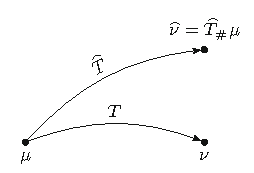
\includegraphics[width=0.29\textwidth]{assets/chapter3/figure-3-1.pdf}
\caption{传输映射之间的 $L^2$ 误差控制 $\widehat\nu$ 与 $\nu$ 之间的 $W_2^2$ 距离.}\label{fig:3.1}
\end{figure}
\begin{figure}[htbp]\centering
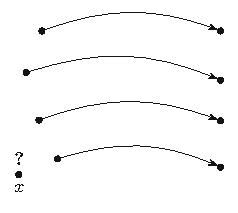
\includegraphics[width=0.28\textwidth]{assets/chapter3/figure-3-2.pdf}
\caption{如何在样本外的点 $x$ 处对经验最优传输映射作插值？}\label{fig:3.2}
\end{figure}

$L^2$ 积分误差是非参数统计中常用的一种自然距离度量. 不过，在这里它还有另一层解释：控制 $\mu$ 在两个映射下的推前测度之间的 Wasserstein 距离. 更准确地说，根据定义 $\nu=T_\#\mu$. 如果通过 $\widehat\nu=\widehat T_\#\mu$ 定义测度 $\widehat\nu$，那么对于 $X\sim\mu$，$(\widehat T(X),T(X))$ 是 $\widehat\nu$ 与 $\nu$ 的一个次优耦合，因而
$$
W_2^2(\widehat\nu,\nu)\le\mathbb E\|\widehat T(X)-T(X)\|^2
=\int\|\widehat T(x)-T(x)\|^2\,\mu(dx).
$$
示意见\autoref{fig:3.1}.

一种初步的估计方法可能是计算经验测度 $\mu_n$ 与 $\nu_n$ 之间的最优耦合，即求解 $\min_{\gamma\in\Gamma_{\mu_n,\nu_n}}\int\|x-y\|^2\,\gamma(dx,dy)$，但我们很快就会发现这一朴素方案存在一个无法回避的缺口. 即使最优传输计划 $\gamma_n$ 由某个传输映射 $T_n$ 诱导，从而 $\gamma_n(dx,dy)=\mu_n(dx)\delta_{T_n(x)}(dy)$，映射 $T_n$ 也仅在样本 $\{X_1,\ldots,X_n\}$ 上有良好定义，尚不清楚如何有原则地将其延拓为整个 $\mathbb R^d$ 上的映射（\autoref{fig:3.2}）. 为解决这一问题，文献中提出了多种方法，旨在构造 $T_n$ 到样本外各点的插值 $\widehat T_n$. 例如，可以令 $\widehat T_n(x)=T_n(X_i)$，其中 $X_i$ 是距离 $x$ 最近的样本点. 这就是 1-最近邻估计量（1-nearest neighbor estimator）；可以证明，在没有额外光滑性假设时，它具有极小极大最优性\cite{ref221}；一维情形见\autoref{exer:3.1}. 不过，这种方法无法利用 $\mu$ 和 $\nu$ 的额外正则性，我们在此不再继续讨论.

相反，下一节将根据最优传输的半对偶表述设计一个估计量. 这一估计策略的优点在于，能够灵活纳入对总体传输映射 $T$ 的额外假设，例如光滑性. 采用足够强的假设，就可以得到避开维数灾难的映射估计量.

\subsection{半对偶问题及其稳定性}\label{sec:3.2}\index{semidual@半对偶（semidual）!stability@稳定性（stability）|hyperpage}
回顾半对偶问题：如果 $\nabla\varphi$ 是最优传输映射，那么 $\varphi$ 极小化
$$\mathcal S(\phi):=\int\phi\,d\mu+\int\phi^*\,d\nu,$$
其中 $\phi^*(y)=\sup_{x\in\mathbb R^d}\{\langle x,y\rangle-\phi(x)\}$ 是 $\phi$ 的凸共轭. 关键在于，半对偶问题可以直接将总体测度 $\mu,\nu$ 替换为对应的经验测度 $\mu_n,\nu_n$，从而自然得到 $\varphi$ 的估计量：令
\begin{equation}\label{eq:3.1}
\widehat\varphi=\operatorname*{arg\,min}_{\phi\in\mathcal F}\mathcal S_n(\phi)
:=\operatorname*{arg\,min}_{\phi\in\mathcal F}\left\{\int\phi\,d\mu_n+\int\phi^*\,d\nu_n\right\},
\end{equation}
其中 $\mathcal F$ 是一个稍后选取的适当函数类. 再令 $\widehat T=\nabla\widehat\varphi$，便得到最优传输映射的估计量. 通过 \eqref{eq:3.1}，我们将传输映射估计问题置于研究充分的经验风险最小化（empirical risk minimization，ERM）框架之中；这一框架是现代统计理论的基石，现代综述可参见\cite{ref318}. 与许多通过经验风险最小化定义的估计量类似，目前尚不清楚能否高效计算 $\widehat T$；不过，这里着重研究传输映射估计的统计方面，而非计算方面.

从统计学的角度看，Brenier 定理的唯一性结论保证最优传输映射 $T$ 可识别，因此统计问题是良定的. 换言之，如果 $\mathcal S(\phi)=\mathcal S(\varphi)$，则 $\nabla\phi=\nabla\varphi$ 在 $\mu$ 几乎处处成立. 不过，为了得到估计速率，需要将这一定性断言加强为稳定性结论，即下面的定理.

\begin{theorem}\label{thm:3.1}
假设 $\phi$ 强凸且光滑，
$$\frac12 I\preceq\nabla^2\phi\preceq2I.$$
那么，
\begin{equation}\label{eq:3.2}
\frac14\|\nabla\phi-\nabla\varphi\|_{L^2(\mu)}^2
\le\mathcal S(\phi)-\mathcal S(\varphi)
\le\|\nabla\phi-\nabla\varphi\|_{L^2(\mu)}^2.
\end{equation}
\end{theorem}

在证明\autoref{thm:3.1}之前，先说明这一稳定性结果如何融入整体统计分析. 该证明是经验风险最小化估计量分析的一种典型范例. 根据定义，$\widehat\varphi$ 极小化 $\mathcal S_n$. 利用经验过程理论的工具，可以控制随机泛函 $\mathcal S_n$ 偏离其均值 $\mathcal S$ 的波动，从而得出 $\mathcal S(\widehat\varphi)-\mathcal S(\varphi)$ 很小. 再由 \eqref{eq:3.2} 的第一个不等式，便可知估计误差 $\|\widehat T-T\|_{L^2(\mu)}^2$ 很小.

实际上，为了得到更快的估计速率，我们还会引入另一项要素来改进这一论证：不动点或局部化技术（fixed-point or localization technique）. 简言之，估计速率依赖于在一个包含估计量 $\widehat\varphi$ 的函数集合上，对 $\mathcal S_n$ 偏离 $\mathcal S$ 的程度作一致控制. 一旦通过稳定性不等式 \eqref{eq:3.2} 知道 $\widehat\varphi$ 接近 $\varphi$，就可以重复这一论证，但将范围限制在更小的函数类内，从而进一步改进估计速率. 在这一通过局部化估计量 $\widehat\varphi$ 不断细化界的迭代过程中，寻找其不动点，就会得到最终估计速率.

现在转向\autoref{thm:3.1}的证明. 我们将反复使用 Fenchel--Young 不等式（\autoref{thm:A.6}），以及 $f$ 的 $\alpha$-凸性等价于 $f^*$ 的 $\alpha^{-1}$-光滑性这一事实（\autoref{lem:A.9}）.

\begin{proof}[\autoref{thm:3.1}的证明]
由于 $(\nabla\varphi)_\#\mu=\nu$，
$$
\begin{aligned}
\mathcal S(\phi)&=\int\phi(x)\,\mu(dx)+\int\phi^*(y)\,\nu(dy)\\
&=\int\bigl(\phi(x)+\phi^*(\nabla\varphi(x))\bigr)\,\mu(dx).
\end{aligned}
$$
由 $\phi^*$ 的强凸性，
$$
\begin{aligned}
\phi^*(\nabla\varphi(x))\ge{}&\phi^*(\nabla\phi(x))
+\langle\underbrace{\nabla\phi^*(\nabla\phi(x))}_{=x},\nabla\varphi(x)-\nabla\phi(x)\rangle\\
&+\frac14\|\nabla\varphi(x)-\nabla\phi(x)\|^2,
\end{aligned}
$$
因而
$$
\begin{aligned}
\phi(x)+\phi^*(\nabla\varphi(x))\ge{}&
\underbrace{\phi(x)+\phi^*(\nabla\phi(x))}_{=\langle x,\nabla\phi(x)\rangle}
+\langle x,\nabla\varphi(x)-\nabla\phi(x)\rangle\\
&+\frac14\|\nabla\varphi(x)-\nabla\phi(x)\|^2\\
={}&\langle x,\nabla\varphi(x)\rangle+\frac14\|\nabla\varphi(x)-\nabla\phi(x)\|^2.
\end{aligned}
$$
另一方面，
$$
\mathcal S(\varphi)=\int\bigl(\varphi(x)+\varphi^*(\nabla\varphi(x))\bigr)\,\mu(dx)
=\int\langle x,\nabla\varphi(x)\rangle\,\mu(dx).
$$
因此得到
$$\mathcal S(\phi)\ge\mathcal S(\varphi)+\frac14\|\nabla\varphi-\nabla\phi\|_{L^2(\mu)}^2.$$
类似地，由光滑性，
$$
\begin{aligned}
\phi^*(\nabla\varphi(x))\le{}&\phi^*(\nabla\phi(x))
+\langle\underbrace{\nabla\phi^*(\nabla\phi(x))}_{=x},\nabla\varphi(x)-\nabla\phi(x)\rangle\\
&+\|\nabla\varphi(x)-\nabla\phi(x)\|^2,
\end{aligned}
$$
因而
$$
\begin{aligned}
\phi(x)+\phi^*(\nabla\varphi(x))\le{}&\phi(x)+\phi^*(\nabla\phi(x))
+\langle x,\nabla\varphi(x)\rangle-\langle x,\nabla\phi(x)\rangle\\
&+\|\nabla\varphi(x)-\nabla\phi(x)\|^2\\
={}&\langle x,\nabla\phi(x)\rangle+\varphi(x)+\varphi^*(\nabla\varphi(x))
-\langle x,\nabla\phi(x)\rangle\\
&+\|\nabla\varphi(x)-\nabla\phi(x)\|^2,
\end{aligned}
$$
积分即得结论.
\end{proof}

注意，我们实际上证明了更强的结论：若写成
$$\mathcal S(\phi)=\int\underbrace{\bigl(\phi(x)+\phi^*(\nabla\varphi(x))\bigr)}_{s_\phi(x)}\,\mu(dx),$$
那么有逐点界
$$\frac14\|\nabla\varphi(x)-\nabla\phi(x)\|^2
\le s_\phi(x)-s_\varphi(x)\le\|\nabla\varphi(x)-\nabla\phi(x)\|^2.$$

\subsection{一个特例：仿射传输映射}\label{sec:3.3}
作为合理性检验，我们先说明半对偶估计技术适用于一个十分简单的问题. 考虑单样本情形（one-sample setting）：$\mu=\mathcal N(0,I)$ 已知，我们从 $\nu=(\nabla\varphi)_\#\mu$ 获得样本，其中某个 $\varphi\in\mathcal F$，而 $\mathcal F$ 由所有凸二次函数 $x\mapsto\frac12 x^{\mathsf T}Ax+b^{\mathsf T}x$、$A\succeq0$ 构成. 若 $\varphi$ 具有这一形式，那么传输映射 $\nabla\varphi$ 就是仿射映射 $Ax+b$，且 $\nu=\mathcal N(b,A^2)$.

在这一情形下，自然可以先计算 $\nu$ 的经验均值 $\widehat m$ 与经验协方差 $\widehat\Sigma$，再令
\begin{equation}\label{eq:3.3}
\widehat T(x)=\widehat\Sigma^{1/2}x+\widehat m.
\end{equation}
文献\cite{ref135}在更一般的情形下研究了这一估计量，利用的是推导协方差矩阵估计速率的技术.

下面的结果说明，\eqref{eq:3.3} 定义的 $\widehat T$ 恰好就是通过极小化经验半对偶泛函所计算出的估计量.

\begin{proposition}\label{prop:3.2}
令 $\mathcal F$ 为 $\mathbb R^d$ 上所有凸二次函数的集合. 设 $\mu=\mathcal N(0,I)$，以 $\nu_n$ 表示由概率测度 $\nu$ 的独立同分布样本构成的经验测度. 如果
$$\widehat\varphi=\operatorname*{arg\,min}_{\phi\in\mathcal F}
\left\{\int\phi\,d\mu+\int\phi^*\,d\nu_n\right\},$$
那么
$$\nabla\widehat\varphi(x)=\widehat\Sigma^{1/2}x+\widehat m,$$
其中 $\widehat m$ 和 $\widehat\Sigma$ 分别为 $\nu_n$ 的均值与协方差.
\end{proposition}
\begin{proof}
根据定义，$\widehat\varphi=\frac12x^{\mathsf T}\widehat A x+\widehat b^{\mathsf T}x$，其中 $(\widehat A,\widehat b)$ 求解
$$
\min_{A\succeq0,\,b\in\mathbb R^d}
\left[\int\left(\frac12x^{\mathsf T}Ax+b^{\mathsf T}x\right)\mu(dx)
+\int\left(\frac12y^{\mathsf T}Ay+b^{\mathsf T}y\right)^*\nu_n(dy)\right].
$$
由\autoref{lem:A.13}，二次函数的凸共轭仍为二次函数，所以第二个积分只依赖于 $\nu_n$ 的至多二阶矩. 因此，可以将关于 $\nu_n$ 的积分替换为关于任何具有相同前两阶矩的测度的积分，特别可以取 $\mathcal N(\widehat m,\widehat\Sigma)$. 于是，由于这一函数类包含高斯分布之间的全部 Kantorovich 势（见\autoref{ex:1.19}），可知极小化解就是对应于从 $\mathcal N(0,I)$ 到 $\mathcal N(\widehat m,\widehat\Sigma)$ 的最优传输的那个函数.
\end{proof}

在\autoref{prop:3.2}的情形下，可以直接分析 $\widehat T$ 的性能，因为它根据样本均值与样本协方差显式定义. 但对更一般的函数族 $\mathcal F$，通常无法显式求解半对偶问题，需要使用更抽象的论证来分析 $\widehat\varphi$.

\subsection{得到慢速率}\label{sec:3.4}
本节和下一节着重估计由适当函数类 $\Phi$ 中的势所产生的映射，要求该类的覆盖数（含义同\autoref{sec:2.3}）得到适当控制. 这些覆盖数的大小直接影响通过极小化经验半对偶、如 \eqref{eq:3.1} 所得到的估计量的质量.

\Needspace{10\baselineskip}
为开始分析，先对测度 $\mu,\nu$ 和函数族 $\Phi$ 作若干技术假设.
\begin{assumption}\label{assump:3.3}
存在 $\varphi\in\Phi$，使得 $\nu=(\nabla\varphi)_\#\mu$，其中 $\mu,\nu$ 和 $\Phi$ 满足：
\begin{itemize}
\item $\mu$ 和 $\nu$ 的支集包含在 $\Omega=B_1(0)$ 中.
\item 集合 $\Phi$ 在 $\Omega$ 上关于 $L^\infty$ 有界，即 $\sup_{\phi\in\Phi}\|\phi\|_{L^\infty(\Omega)}\lesssim1$.
\item 势满足 $\phi(0)=0$，且当 $x\notin\Omega$ 时 $\phi(x)=+\infty$.
\item 势处处下半连续，且在 $\Omega$ 上光滑并强凸：当 $\|x\|<1$ 时，$\frac12 I\preceq\nabla^2\phi(x)\preceq2I$.
\end{itemize}
\end{assumption}
在适当强的矩假设下，前两个假设可以减弱，但这里不沿这一方向展开. 第三个假设不失一般性：从 $\phi$ 中减去常数不影响半对偶目标函数或梯度 $\nabla\phi$，所以总可以假设 $\phi(0)=0$；而由于 $\mu$ 和 $\nu$ 的支集包含在 $B_1(0)$ 内，可以将 $\phi$ 在这一集合之外定义为无穷大，而不影响半对偶问题. $\phi$ 在 $\Omega$ 外恒等于 $+\infty$，会简化若干涉及共轭函数的论证，因为它意味着，对所有 $y\in\mathbb R^d$ 和 $\phi\in\Phi$，
$$\phi^*(y)=\sup_{x\in\mathbb R^d}\{\langle x,y\rangle-\phi(x)\}
=\sup_{x\in\Omega}\{\langle x,y\rangle-\phi(x)\}.$$
第四个假设最为重要，因为它通过\autoref{thm:3.1}保证半对偶问题的稳定性.

有了这些假设，就可以开展分析的第一步.
\begin{lemma}\label{lem:3.4}
采用\autoref{assump:3.3}，并假设对某个 $\varphi\in\Phi$ 有 $\nu=\nabla\varphi_\#\mu$. 令 $\widehat\varphi$ 为
$$\widehat\varphi=\operatorname*{arg\,min}_{\phi\in\Phi}\mathcal S_n(\phi).$$
那么
\begin{equation}\label{eq:3.4}
\|\nabla\widehat\varphi-\nabla\varphi\|_{L^2(\mu)}^2
\lesssim\sup_{\phi\in\Phi}\{|(\mu_n-\mu)(\phi)|+|(\nu_n-\nu)(\phi^*)|\}.
\end{equation}
\end{lemma}
\begin{proof}
这是经验风险最小化中一种标准论证的应用. \autoref{thm:3.1}给出
$$\begin{aligned}
\|\nabla\widehat\varphi-\nabla\varphi\|_{L^2(\mu)}^2
&\lesssim\mathcal S(\widehat\varphi)-\mathcal S(\varphi)\\
&=\mathcal S(\widehat\varphi)-\mathcal S_n(\widehat\varphi)
+\mathcal S_n(\widehat\varphi)-\mathcal S_n(\varphi)\\
&\quad+\mathcal S_n(\varphi)-\mathcal S(\varphi)\\
&\le2\sup_{\phi\in\Phi}|\mathcal S_n(\phi)-\mathcal S(\phi)|,
\end{aligned}$$
最后一步不等式利用了根据 $\widehat\varphi$ 的定义有 $\mathcal S_n(\widehat\varphi)-\mathcal S_n(\varphi)\le0$. 展开 $\mathcal S$ 与 $\mathcal S_n$ 的定义即得结论.
\end{proof}

为控制 \eqref{eq:3.4} 的右端，使用\autoref{prop:2.6}的链式技术. 为简单起见，着重考虑函数类足够小、使得对所有充分小的 $\varepsilon$ 都有
\begin{equation}\label{eq:3.5}
\log N(\varepsilon,\Phi)\lesssim\varepsilon^{-\gamma}\log(1+\varepsilon^{-1}),\qquad\gamma\in[0,1)
\end{equation}
的情形.

参数类是这种函数类的典型例子，即集合 $\Phi$ 有限维：$\Phi=\{\phi_\theta\}_{\theta\in\Theta}$ 由参数 $\theta\in\Theta\subseteq\mathbb R^M$ 索引. 事实上，这时有下述界.
\begin{lemma}\label{lem:3.5}
假设 $\Phi=\{\phi_\theta\}_{\theta\in\Theta}$，其中 $\Theta\subseteq\mathbb R^M$ 有界，且势满足 $\|\phi_\theta-\phi_{\theta'}\|_{L^\infty(\Omega)}\lesssim\|\theta-\theta'\|$. 则存在正常数 $C$，使得当 $\varepsilon\ge C$ 时，$\Phi$ 的覆盖数满足 $\log N(\varepsilon,\Phi)=0$；在其他情形，
$$\log N(\varepsilon,\Phi)\lesssim\log(1+\varepsilon^{-1}).$$
\end{lemma}
\begin{proof}
根据假设，对某个 $R>0$ 有 $\Theta\subseteq B_R(0)$，所以对任意 $\phi,\psi\in\Phi$ 有 $\|\phi-\psi\|_{L^\infty(\Omega)}\lesssim R$. 因此，如果 $\varepsilon$ 大于一个足够大的常数，则 $\Phi$ 的任意元素都构成 $\Phi$ 的单元素 $\varepsilon$-覆盖.

对任意 $\delta>0$，\autoref{exer:3.2}表明存在 $\theta_1,\ldots,\theta_N$，其中 $N\le(1+2R\delta^{-1})^M$，使得 $\bigcup_{i=1}^N B_\delta(\theta_i)\supseteq\Theta$. 于是 $\phi_{\theta_1},\ldots,\phi_{\theta_N}$ 是 $\Phi$ 的一个 $O(\delta)$-覆盖. 事实上，对任意 $\theta\in\Theta$，可以选取 $i\in[N]$，使得 $\|\phi_\theta-\phi_{\theta_i}\|_{L^\infty(\Omega)}\lesssim\|\theta-\theta_i\|\le\delta$. 对充分小的正常数 $c$ 取 $\delta=c\varepsilon$，即得所述结论.
\end{proof}

举一些参数类的例子：$\{\phi_\theta\}_{\theta\in\Theta}$ 可以是\autoref{sec:3.3}中的凸二次函数集合，也可以由固定字典（dictionary）$\{\phi_1,\ldots,\phi_M\}$ 的线性组合构成：
$$\phi_\theta=\sum_{i=1}^M\theta_i\phi_i.$$
注意，非参数统计中通常会精心选择字典，以平衡逼近误差与估计误差；不过，为了集中讨论核心统计内容，这里不深入研究这些问题.

更一般地，条件 \eqref{eq:3.5} 允许无限维、但仍然“不太大”的函数类. 相比之下，它排除了复杂度随环境维数增长的类，例如\autoref{lem:2.7}研究的 Lipschitz 函数类.

在这一假设下，估计 $T=\nabla\varphi$ 的最优速率是什么？如果 $\Phi$ 是参数类，我们预期极小极大速率为 $n^{-1}$；特别地，我们预期映射估计问题可以避开维数灾难. 事实上，只要满足形如 \eqref{eq:3.5} 的界，就能够达到避开维数灾难的速率.

\autoref{lem:3.4}同时涉及势 $\phi$ 及其共轭 $\phi^*$. 遗憾的是，即使集合 $\Phi$ 具有简单形式，集合 $\Phi^*=\{\phi^*: \phi\in\Phi\}$ 也可能难以简洁描述. 不过，我们有下面这个关键观察：$\Phi$ 的覆盖数控制 $\Phi^*$ 的覆盖数.
\begin{lemma}\label{lem:3.6}
对任意 $\varepsilon>0$，
$$N(\varepsilon,\Phi^*)\le N(\varepsilon,\Phi).$$
\end{lemma}
\begin{proof}
这是共轭运算在 $L^\infty$ 中具有压缩性这一事实的结果. 事实上，给定任意函数对 $\phi,\psi\in\Phi$，
$$\begin{aligned}
|\phi^*(y)-\psi^*(y)|
&=\left|\sup_{x\in\Omega}\{\langle x,y\rangle-\phi(x)\}
-\sup_{x'\in\Omega}\{\langle x',y\rangle-\psi(x')\}\right|\\
&\le\sup_{x\in\Omega}|\phi(x)-\psi(x)|=\|\phi-\psi\|_{L^\infty(\Omega)}.
\end{aligned}$$
特别地，如果 $\phi_1,\ldots,\phi_N$ 是 $\Phi$ 的一个 $\varepsilon$-网，那么 $\phi_1^*,\ldots,\phi_N^*$ 是 $\Phi^*$ 的一个 $\varepsilon$-网.
\end{proof}

现在可以证明映射估计的第一个收敛速率.
\begin{theorem}\label{thm:3.7}
采用\autoref{assump:3.3}，并假设 \eqref{eq:3.5} 成立. 半对偶估计量 $\widehat\varphi$ 满足
$$\mathbb E\|\nabla\widehat\varphi-\nabla\varphi\|_{L^2(\mu)}^2\lesssim n^{-1/2}.$$
\end{theorem}
\begin{proof}
\autoref{lem:3.4}给出
$$\begin{aligned}
\mathbb E\|\nabla\widehat\varphi-\nabla\varphi\|_{L^2(\mu)}^2
\lesssim{}&\mathbb E\sup_{\phi\in\Phi}|(\mu_n-\mu)(\phi)|\\
&+\mathbb E\sup_{\phi\in\Phi}|(\nu_n-\nu)(\phi^*)|.
\end{aligned}$$
由\autoref{assump:3.3}，存在正常数 $R$，使得对所有 $\phi\in\Phi$，$\|\phi\|_{L^\infty(\Omega)}\le R$ 且 $\|\phi^*\|\le R$. 在\autoref{prop:2.6}中取 $\tau=0$，得到
$$\mathbb E\|\nabla\widehat\varphi-\nabla\varphi\|_{L^2(\mu)}^2
\lesssim\frac1{\sqrt n}\int_0^R
\left(\sqrt{\log N(\varepsilon,\Phi)}+\sqrt{\log N(\varepsilon,\Phi^*)}\right)d\varepsilon.$$
应用 \eqref{eq:3.5} 和\autoref{lem:3.6}，可得
$$\mathbb E\|\nabla\widehat\varphi-\nabla\varphi\|_{L^2(\mu)}^2
\lesssim\frac1{\sqrt n}\int_0^R\varepsilon^{-\gamma/2}
\sqrt{\log(1+\varepsilon^{-1})}\,d\varepsilon\lesssim n^{-1/2},$$
即为所求.
\end{proof}

正如预期，对类 $\Phi$ 的参数化假设带来了避开维数灾难的收敛速率. 不过，“慢速率”$n^{-1/2}$ 尚未达到希望证明的结果. 为得到“快速率”$n^{-1}$，需要进行局部化；要利用这一步局部化，还必须对 $\mu$ 施加额外假设.

\subsection{不动点论证}\label{sec:3.5}
如上所述，\autoref{thm:3.7}中的链式论证未能给出正确的收敛速率，因为它在整个集合 $\Phi$ 上一致控制 $\mathcal S_n$ 偏离 $\mathcal S$ 的程度. 不过，\autoref{thm:3.7}表明，当 $n$ 较大时 $\widehat\varphi$ 接近 $\varphi$，这提示我们没有必要在整个 $\Phi$ 上一致控制偏离程度，而只需在 $\varphi$ 附近的子集上进行控制.

下面由 van de Geer 提出的论证，将这一过程在映射估计背景下严格化. 核心思想不是将\autoref{lem:3.4}的推理用于 $\widehat\varphi$，而是用于 $\widehat\varphi$ 与 $\varphi$ 本身的一个凸组合. 为简单起见，应用这一论证时，对 $\Phi$ 再增加一个假设.
\begin{assumption}\label{assump:3.8}
集合 $\Phi$ 是凸的，即若 $\phi,\psi\in\Phi$，则对所有 $\lambda\in[0,1]$，有 $(1-\lambda)\phi+\lambda\psi\in\Phi$.
\end{assumption}
定义
$$\varphi_\varepsilon=(1-\lambda)\varphi+\lambda\widehat\varphi,
\qquad\lambda=\frac{\varepsilon}{\varepsilon+\|\nabla\widehat\varphi-\nabla\varphi\|_{L^2(\mu)}}.$$
那么，
$$\begin{aligned}
\|\nabla\varphi_\varepsilon-\nabla\varphi\|_{L^2(\mu)}
&=\lambda\|\nabla\widehat\varphi-\nabla\varphi\|_{L^2(\mu)}\\
&=\varepsilon\left(\frac{\|\nabla\widehat\varphi-\nabla\varphi\|_{L^2(\mu)}}
{\varepsilon+\|\nabla\widehat\varphi-\nabla\varphi\|_{L^2(\mu)}}\right)\le\varepsilon.
\end{aligned}$$
此外，
$$\begin{aligned}
\|\nabla\varphi_\varepsilon-\nabla\varphi\|_{L^2(\mu)}\le\frac\varepsilon2
&\iff\frac{\varepsilon\|\nabla\widehat\varphi-\nabla\varphi\|_{L^2(\mu)}}
{\varepsilon+\|\nabla\widehat\varphi-\nabla\varphi\|_{L^2(\mu)}}\le\frac\varepsilon2\\
&\iff\|\nabla\widehat\varphi-\nabla\varphi\|_{L^2(\mu)}\le\varepsilon,
\end{aligned}$$
所以，用 $\|\nabla\varphi_\varepsilon-\nabla\varphi\|_{L^2(\mu)}$ 代替 $\|\nabla\widehat\varphi-\nabla\varphi\|_{L^2(\mu)}$，只损失一个因子 2. 最后，\autoref{assump:3.8}保证 $\varphi_\varepsilon\in\Phi$，因为它是 $\Phi$ 中元素的凸组合.

还要注意，对 $\lambda\in[0,1]$，逐点有 $((1-\lambda)\phi_0+\lambda\phi_1)^*\le(1-\lambda)\phi_0^*+\lambda\phi_1^*$，由此可知 $\mathcal S_n$ 是凸泛函. 若令 $\overline{\mathcal S}=\mathcal S-\mathcal S(\varphi)$ 和 $\overline{\mathcal S_n}=\mathcal S_n-\mathcal S_n(\varphi)$，那么由凸性及 $\widehat\varphi$ 的定义，
$$\overline{\mathcal S_n}(\varphi_\varepsilon)
\le(1-\lambda)\underbrace{\overline{\mathcal S_n}(\varphi)}_{=0}
+\lambda\underbrace{\overline{\mathcal S_n}(\widehat\varphi)}_{\le0}\le0.$$
因此，由\autoref{thm:3.1}，若 $\varphi_\varepsilon$ 是 $\frac12$-强凸且 2-光滑的，则
$$\begin{aligned}
\frac14\|\nabla\varphi_\varepsilon-\nabla\varphi\|_{L^2(\mu)}^2
&\le\overline{\mathcal S}(\varphi_\varepsilon)
\le(\overline{\mathcal S}-\overline{\mathcal S_n})(\varphi_\varepsilon)\\
&=(\mathcal S-\mathcal S_n)(\varphi_\varepsilon)-(\mathcal S-\mathcal S_n)(\varphi)\\
&\le\sup_{\phi\in\Phi_\varepsilon}(\mathcal S-\mathcal S_n)(\phi)
-(\mathcal S-\mathcal S_n)(\varphi)\\
&\le\sup_{\phi\in\Phi_\varepsilon}
\{|(\mu_n-\mu)(\phi-\varphi)|+|(\nu_n-\nu)(\phi^*-\varphi^*)|\},
\end{aligned}$$
其中 $\Phi_\varepsilon=\{\phi\in\Phi:\|\nabla\phi-\nabla\varphi\|_{L^2(\mu)}\le\varepsilon\}$.

如果上述不等式右端小于 $\varepsilon^2/16$，那么 $\|\nabla\varphi_\varepsilon-\nabla\varphi\|_{L^2(\mu)}\le\varepsilon/2$，进而有 $\|\nabla\widehat\varphi-\nabla\varphi\|_{L^2(\mu)}\le\varepsilon$. 因此，如果能找到一个 $\varepsilon$，使经验过程在 $\mathcal F_\varepsilon$ 上的上确界具有 $\varepsilon^2$ 的量级，就可以控制 $\widehat\varphi$ 的风险. 下面的命题将这些讨论严格化.
\begin{proposition}\label{prop:3.9}
采用\autoref{assump:3.3}和\autoref{assump:3.8}. 对 $\varepsilon>0$，令
$$r(\varepsilon)=\sup_{\phi\in\Phi_\varepsilon}
\{|(\mu_n-\mu)(\phi-\varphi)|+|(\nu_n-\nu)(\phi^*-\varphi^*)|\}.$$
那么，在事件 $\{r(\varepsilon)\le\varepsilon^2/16\}$ 上，半对偶估计量 $\widehat\varphi$ 满足 $\|\nabla\widehat\varphi-\nabla\varphi\|_{L^2(\mu)}\le\varepsilon$.

特别地，如果 $\varepsilon_n$ 是确定性量，且以高概率有 $r(\varepsilon_n)\le\varepsilon_n^2/16$，那么以高概率，$\widehat\varphi$ 的风险由 $\varepsilon_n$ 控制.
\end{proposition}

比较\autoref{lem:3.4}和\autoref{prop:3.9}可见，我们已将在 $\Phi$ 上一致控制经验过程偏差的任务，替换为在更小集合 $\Phi_\varepsilon$ 上控制偏差的任务.

\subsection{得到快速率}\label{sec:3.6}
为了利用现在只需在 $\Phi_\varepsilon$ 上控制经验过程这一事实，需要严格表述 $\Phi_\varepsilon$ 比 $\Phi$ 小得多的含义. 一个复杂因素在于，\autoref{prop:2.6}中的链式技术通过 $\varepsilon$-覆盖数度量 $\Phi$ 的“大小”，而这些覆盖数是根据 $L^\infty$ 覆盖定义的. 相比之下，将 $\Phi$ 限制为 $\Phi_\varepsilon$，依据的是对 $\phi$ 的梯度的 $L^2$ 范数施加额外限制. 因此，需要一种能够同时利用函数类在 $L^\infty$ 和 $L^2$ 意义下的大小的链式界.

下面修改后的链式界弥补了这一不足.
\begin{proposition}[{\cite[定理2.14.21]{ref309}}]\label{prop:3.10}
设 $P$ 是集合 $\Omega\subseteq\mathbb R^d$ 上的概率测度，$X_1,\ldots,X_n\overset{\mathrm{i.i.d.}}\sim P$. 若 $\mathcal F$ 是一组实值函数，且对所有 $f\in\mathcal F$ 有 $\|f\|_{L^2(P)}\le\sigma$、$\|f\|_{L^\infty(\Omega)}\le R$，则
\begin{equation}\label{eq:3.6}
\begin{aligned}
\mathbb E\sup_{f\in\mathcal F}\frac1n\sum_{i=1}^n\{f(X_i)-\mathbb Ef(X_i)\}
\lesssim{}&\frac1{\sqrt n}\int_0^\sigma\sqrt{\log N(\varepsilon,\mathcal F)}\,d\varepsilon\\
&+\frac1n\int_0^R\log N(\varepsilon,\mathcal F)\,d\varepsilon.
\end{aligned}
\end{equation}
\end{proposition}
注意，在 \eqref{eq:3.6} 第一项中，积分上限为 $\sigma$ 而不是 $R$. 第二个积分对覆盖数的依赖较差，但其前置因子为 $1/n$，而非 $1/\sqrt n$. 因此可以期待，当 $n$ 足够大时，第一项占主导地位. 如果 $\mathcal F$ 的 $L^2$ 大小很小，即 $\sigma$ 很小，那么第一项可能显著小于直接应用\autoref{prop:2.6}得到的界.

\autoref{prop:3.10}还附带一个尾界，说明 \eqref{eq:3.6} 右端也以高概率控制经验过程.
\begin{proposition}\label{prop:3.11}
以 $J_n(\mathcal F)$ 表示 \eqref{eq:3.6} 的右端. 在与\autoref{prop:3.10}相同的假设下，存在正常数 $C$，它是普适常数，使得对任意 $t\ge0$，
$$\mathbb P\left(\sup_{f\in\mathcal F}\frac1n\sum_{i=1}^n\{f(X_i)-\mathbb Ef(X_i)\}
\ge C\left(J_n(\mathcal F)+\sigma\sqrt{\frac tn}+R\frac tn\right)\right)\le e^{-t}.$$
\end{proposition}

\autoref{prop:3.10}要求控制函数类元素的 $L^2$ 范数，但 $\Phi_\varepsilon$ 是用 $\Phi$ 中元素的梯度的 $L^2$ 范数定义的. 因此，我们对 $\mu$ 采用最后一个假设，使我们可以在这两种概念之间转换.
\begin{definition}\label{def:3.12}\index{Poincaré inequality@Poincaré不等式（Poincaré inequality）|hyperpage}
如果对所有 $f\in L^2(P)$ 有
$$\int\left(f-\int f\,dP\right)^2dP\le C\int\|\nabla f\|^2\,dP,$$
则称测度 $P$ 满足 Poincar\'e 不等式（Poincar\'e inequality），其常数为 $C$.
\end{definition}
\begin{assumption}\label{assump:3.13}
测度 $\mu$ 满足 Poincar\'e 不等式.
\end{assumption}

Poincar\'e 不等式是“$\mu$ 的支集连通”这一断言的定量形式. 事实上，若一个测度在有界 Lipschitz 区域上具有远离零且有界的密度，它就满足 Poincar\'e 不等式.

在这一新假设下，可以得到 $\Phi_\varepsilon$ 和 $\Phi_\varepsilon^*$ 的 $L^2$ 界.
\begin{proposition}\label{prop:3.14}
若\autoref{assump:3.3}和\autoref{assump:3.13}成立，则对所有 $\phi\in\Phi_\varepsilon$，
$$\|\phi-\varphi-\mu(\phi-\varphi)\|_{L^2(\mu)}\lesssim\varepsilon,$$
$$\|\phi^*-\varphi^*-\nu(\phi^*-\varphi^*)\|_{L^2(\nu)}\lesssim\varepsilon.$$
\end{proposition}
\begin{proof}
第一个界直接由 Poincar\'e 不等式得到：对 $\phi\in\Phi_\varepsilon$，
$$\|\phi-\varphi-\mu(\phi-\varphi)\|_{L^2(\mu)}^2
\le C\|\nabla(\phi-\varphi)\|_{L^2(\mu)}^2\lesssim\varepsilon^2.$$

为证明第二个界，先利用 $\phi$ 和 $\varphi$ 的强凸性. 考虑泛函 $\mathcal T$，定义为
$$\mathcal T(\psi):=\int\psi\,d\nu+\int\psi^*\,d\mu.$$
即 $\mathcal T$ 是交换 $\mu$ 与 $\nu$ 的角色后得到的半对偶泛函. 由于对所有凸且下半连续的 $\phi$，都有 $(\phi^*)^*=\phi$，所以对所有这样的 $\phi$，有 $\mathcal S(\phi)=\mathcal T(\phi^*)$. 特别地，$\mathcal T$ 的极小化解为 $\varphi^*$，由\autoref{thm:3.1}可知
$$\begin{aligned}
\frac14\|\nabla\phi^*-\nabla\varphi^*\|_{L^2(\nu)}^2
&\le\mathcal T(\phi^*)-\mathcal T(\varphi^*)\\
&=\mathcal S(\phi)-\mathcal S(\varphi)
\le\|\nabla\phi-\nabla\varphi\|_{L^2(\mu)}^2.
\end{aligned}$$
因此，对所有 $\phi\in\Phi_\varepsilon$，有 $\|\nabla\phi^*-\nabla\varphi^*\|_{L^2(\nu)}^2\lesssim\varepsilon^2$.

为了得到所需的界，只需再证明 $\nu$ 也满足 Poincar\'e 不等式，这样便可以像证明第一个不等式那样得出结论. 为此，利用 $\nu=(\nabla\varphi)_\#\mu$. $\varphi$ 的光滑性意味着，对任意 $f:\mathbb R^d\to\mathbb R^d$，
$$\begin{aligned}
\|\nabla(f\circ\nabla\varphi)(x)\|
&=\|\nabla^2\varphi(x)\nabla f(\nabla\varphi(x))\|\\
&\le2\|\nabla f(\nabla\varphi(x))\|.
\end{aligned}$$
$\mu$ 的 Poincar\'e 不等式意味着，对任意 $f\in L^2(\nu)$，
$$\begin{aligned}
\int\left(f-\int f\,d\nu\right)^2d\nu
&=\int\left(f\circ\nabla\varphi-\int f\circ\nabla\varphi\,d\mu\right)^2d\mu\\
&\le C\int\|\nabla(f\circ\nabla\varphi)\|^2\,d\mu\\
&\le4C\int\|\nabla f(\nabla\varphi(x))\|^2\,d\mu\\
&=4C\int\|\nabla f\|^2\,d\nu.
\end{aligned}$$
所以 $\nu$ 也满足常数为 $4C$ 的 Poincar\'e 不等式. 从而可像第一种情形那样得出结论.
\end{proof}

终于可以证明所需的速率了. 注意，在\autoref{lem:3.5}成立的有限维情形下，这一定理说明可以以接近参数速率的速度估计映射.
\begin{theorem}\label{thm:3.15}
采用\autoref{assump:3.3}、\autoref{assump:3.8}和\autoref{assump:3.13}. 如果 \eqref{eq:3.5} 成立，则半对偶估计量 $\widehat\varphi$ 以至少 $1-e^{-t}$ 的概率满足
\begin{equation}\label{eq:3.7}
\|\nabla\widehat\varphi-\nabla\varphi\|_{L^2(\mu)}^2
\lesssim\left(\frac{\log n}n\right)^{\frac2{2+\gamma}}+\frac{t+1}n.
\end{equation}
特别地，
$$\mathbb E\|\nabla\widehat\varphi-\nabla\varphi\|_{L^2(\mu)}^2
\lesssim\left(\frac{\log n}n\right)^{\frac2{2+\gamma}}.$$
\end{theorem}
\begin{proof}
由\autoref{prop:3.9}，只需证明：对于 $\varepsilon_n\asymp(\log n/n)^{1/(2+\gamma)}+\sqrt{(t+1)/n}$，以至少 $1-e^{-t}$ 的概率有 $r(\varepsilon_n)\le\varepsilon_n^2/16$. 先控制 $\sup_{\phi\in\Phi_\varepsilon}|(\mu_n-\mu)(\phi-\varphi)|$. 因为当 $h$ 为常函数时 $(\mu_n-\mu)h=0$，所以
$$\sup_{\phi\in\Phi_\varepsilon}|(\mu_n-\mu)(\phi-\varphi)|
=\sup_{\phi\in\Phi_\varepsilon}|(\mu_n-\mu)(\phi-\varphi-\mu(\phi-\varphi))|.$$
可以应用\autoref{prop:3.10}、\autoref{prop:3.11}和\autoref{prop:3.14}，并利用 $\phi-\varphi-\mu(\phi-\varphi)$ 有界这一事实，得到：存在常数 $C_2$，使得以至少 $1-e^{-t}$ 的概率，
$$\begin{aligned}
&\sup_{\phi\in\Phi_\varepsilon}|(\mu_n-\mu)(\phi-\varphi-\mu(\phi-\varphi))|\\
&\quad\lesssim\frac1{\sqrt n}\int_0^{C_2\varepsilon}
\delta^{-\gamma/2}\sqrt{\log(1+\delta^{-1})}\,d\delta\\
&\qquad+\frac1n\int_0^{C_2}\delta^{-\gamma}\log(1+\delta^{-1})\,d\delta
+\varepsilon\sqrt{\frac tn}+\frac tn\\
&\quad\lesssim\varepsilon^{1-\gamma/2}\sqrt{\frac{\log(1+\varepsilon^{-1})}n}
+\varepsilon\sqrt{\frac tn}+\frac{t+1}n.
\end{aligned}$$
因此，对充分大的常数 $C$，取
\begin{equation}\label{eq:3.8}
\varepsilon_n=C\left(\left(\frac{\log n}n\right)^{\frac1{2+\gamma}}
+\sqrt{\frac{t+1}n}\right),
\end{equation}
就能保证以至少 $1-e^{-t}/2$ 的概率，有
$$\sup_{\phi\in\Phi_{\varepsilon_n}}|(\mu_n-\mu)(\phi-\varphi-\mu(\phi-\varphi))|
\le\varepsilon_n^2/32.$$
类似的论证给出，以同样的概率，
$$\sup_{\phi\in\Phi_{\varepsilon_n}}|(\nu_n-\nu)(\phi^*-\varphi^*-\nu(\phi^*-\varphi^*))|
\le\varepsilon_n^2/32.$$
由并集界，对 \eqref{eq:3.8} 中的 $\varepsilon_n$ 有 $r(\varepsilon_n)\le\varepsilon_n^2/16$，即为所求.

第二个界由对尾部积分得到.
\end{proof}

\subsection{讨论}\label{sec:3.7}
\noindent\textbf{\autoref{sec:3.1}.} 基于最近邻的经验“代入”（plug-in）方法在文献\cite{ref104,ref147,ref221}中发展起来，作为半对偶方法的一个简单替代方案. 最近邻估计量虽然不适应 $\mu$ 和 $\nu$ 的光滑性，但通过密度估计量之间的最优传输映射，可以重新得到极小极大速率\cite{ref221}，甚至得到中心极限定理\cite{ref223}. 不过，与代入方法相比，这里发展的半对偶方法总体上更灵活，可以与核平方和（kernel SoS）等其他工具结合\cite{ref305}.

\noindent\textbf{\autoref{sec:3.2}.} 映射估计的半对偶方法由论文\cite{ref166}引入；该文还证明了半对偶稳定性估计与极小极大下界. 该文表明，如果假设 $\mu$ 与 $\nu$ 之间的映射是 $s$-光滑的，即具有 $s$ 阶有界导数，那么适当的半对偶估计量达到极小极大最优速率
\begin{equation}\label{eq:3.9}
\mathbb E\|\nabla\widehat\varphi-\nabla\varphi\|_{L^2(\mu)}^2
\lesssim n^{-\frac{2\alpha}{2\alpha-2+d}}(\log n)^2+\frac1n.
\end{equation}
此后，文献\cite{ref112}极其一般地研究了这一方法，该文中的论证与本章的论证密切相关. 不过，这里介绍的工具尚不足以证明 \eqref{eq:3.9}，因为 $s$-光滑函数类不满足 \eqref{eq:3.5}. 关于如何沿本章论证的思路得到 \eqref{eq:3.9}，更多信息见\cite[第4.4节]{ref112}.

\autoref{exer:3.3}和\autoref{exer:3.5}中另外两种半对偶稳定性估计取自\cite{ref221}.

\noindent\textbf{\autoref{sec:3.3}.} 文献\cite{ref112}将高斯分布之间的传输映射估计作为半对偶方法给出参数速率的一个例子；其他感兴趣的函数类可参见该文.

\noindent\textbf{\autoref{sec:3.4}.} 经验风险最小化或 M-估计（M-estimation）的标准参考文献包括\cite{ref308,ref318}. “慢速率”是缺乏强凸性时 M-估计问题的典型特征；\autoref{sec:3.6}采用的 Poincar\'e 不等式假设，可以视为半对偶泛函 $\mathcal S$ 的适当强凸性条件.

\noindent\textbf{\autoref{sec:3.5}.} 所用的一次性局部化（one-shot localization）来自 van de Geer\cite{ref306,ref307}，为通常的局部化论证（例如\cite[第14章]{ref318}）提供了替代方法.

\noindent\textbf{\autoref{sec:3.6}.} \autoref{prop:3.10}中改进的链式界由 Talagrand 发展的“一般链式法”（generic chaining）\cite{ref298}得到. 这一技术是高斯过程研究的核心，见\cite{ref299}. \autoref{prop:3.11}的尾界来自关于一般链式界的一个更广泛结果\cite[定理2.2.19]{ref309}.

Poincar\'e 不等式是高维概率中的标准工具，见\cite{ref30,ref51,ref310}. 能否不作这一假设而达到本章给出的速率，目前仍是一个开放问题.

\subsection{习题}\label{sec:3.8}
\begin{exercise}\label{exer:3.1}
设 $\mu,\nu\in\mathcal P([0,1])$，$X_1,\ldots,X_n\sim\mu$、$Y_1,\ldots,Y_n\sim\nu$ 是相互独立的两组独立同分布样本. 假设 $\mu,\nu$ 分别具有可微的累积分布函数 $F_\mu,F_\nu$，且
$$0<c\le F_\mu',F_\nu'\le C<\infty\qquad\text{在 }[0,1]\text{ 上}.$$
这等价于 $\mu,\nu$ 在 $[0,1]$ 上有远离零且有界的密度.

我们来证明下面的估计量 $\widehat T_n$ 满足参数收敛速率. 以 $X_{(1)}<\cdots<X_{(n)}$、$Y_{(1)}<\cdots<Y_{(n)}$ 表示排序后的样本；给定 $x\in[0,1]$，令 $X_{(i)}$ 为来自 $\mu$ 且满足 $X_{(i)}\le x$ 的最大样本. 令 $\widehat T_n(x):=Y_{(i)}$；如果不存在这样的 $X_{(i)}$，则输出 $\widehat T_n(x):=0$. 这一估计量可以视为对经验最优耦合的分段常数插值，也可以视为一个 1-最近邻估计量. 为简单起见，固定 $x\in[0,1]$，并证明
$$\mathbb E[|\widehat T_n(x)-T(x)|^2]\lesssim1/n,$$
其中 $T$ 是从 $\mu$ 到 $\nu$ 的真实最优传输映射 $F_\nu^{-1}\circ F_\mu$；将本题结果推广到积分风险 $\mathbb E\int|\widehat T_n-T|^2\,d\mu$ 也是一个直接的练习.
\begin{enumerate}\renewcommand{\labelenumi}{(\alph{enumi})}
\item 令 $N_x:=\sum_{i=1}^n\mathbbm{1}\{X_i\le x\}$、$N_y':=\sum_{i=1}^n\mathbbm{1}\{Y_i\le y\}$. 说明：若 $N_y'<N_x$，则 $\widehat T_n(x)\ge y$；若 $N_y'>N_x$，则 $\widehat T_n(x)\le y$.
\item 利用 Dvoretzky--Kiefer--Wolfowitz 不等式，说明对任意 $\delta\in(0,1)$，以下结论以至少 $1-\delta$ 的概率同时成立：
$$|N_x-nF_\mu(x)|\lesssim\sqrt{n\log(1/\delta)}$$
以及
$$|N_y'-nF_\nu(y)|\lesssim\sqrt{n\log(1/\delta)}\qquad\text{对所有 }y\in[0,1].$$
\item 利用前两问得出结论.
\end{enumerate}
\end{exercise}

\begin{exercise}\label{exer:3.2}
本题证明，$\mathbb R^d$ 中的球 $B_R(0)$ 可以由 $(1+2R\delta^{-1})^d$ 个半径为 $\delta$ 的球覆盖.
\begin{enumerate}\renewcommand{\labelenumi}{(\alph{enumi})}
\item 利用缩放说明，只需考虑 $R=1$ 的情形.
\item 令 $\mathcal X=\{x_1,\ldots,x_N\}$ 为 $B_1(0)$ 中的任意一组元素，满足对所有 $i\ne j$，有 $\|x_i-x_j\|>\delta$. 这样的集合称为 $B_1(0)$ 的一个 $\delta$-填充（$\delta$-packing）. 证明：若 $\mathcal X$ 是 $B_1(0)$ 的一个 $\delta$-填充，则集合族 $\{B_{\delta/2}(x)\}_{x\in\mathcal X}$ 是 $B_{1+\delta/2}(0)$ 中两两不交的子集. 推出 $|\mathcal X|\le(1+2\delta^{-1})^d$.
\item 假设 $\mathcal X$ 是 $B_R(0)$ 的一个极大 $\delta$-填充，即不存在严格包含 $\mathcal X$ 且仍为 $\delta$-填充的集合. 利用逆否命题说明，$B_R(0)\subseteq\bigcup_{x\in\mathcal X}B_\delta(x)$.
\item 利用前两问得出结论.
\end{enumerate}
\end{exercise}

\begin{exercise}\label{exer:3.3}
设 $\mu,\nu$ 为 $\mathbb R^d$ 上的概率测度，$\nabla\varphi$ 表示从 $\mu$ 到 $\nu$ 的最优传输映射. 假设 $\nabla\varphi$ 为 $L$-Lipschitz. 本题建立下述估计：对任意其他凸函数 $\phi$，若 $\widehat\nu:=(\nabla\phi)_\#\mu$，则
$$\begin{aligned}
\|\nabla\phi-\nabla\varphi\|_{L^2(\mu)}^2
\le L\biggl(&W_2^2(\mu,\widehat\nu)-W_2^2(\mu,\nu)\\
&-\int(\|\cdot\|^2-2\varphi^*)\,d(\widehat\nu-\nu)\biggr).
\end{aligned}$$
\emph{提示：}首先，利用 $\varphi^*$ 的强凸性说明
$$\begin{aligned}
\frac1{2L}\|\nabla\phi-\nabla\varphi\|_{L^2(\mu)}^2
\le{}&\int\varphi^*\,d(\widehat\nu-\nu)\\
&-\int\langle x,\nabla\phi(x)-\nabla\varphi(x)\rangle\,\mu(dx).
\end{aligned}$$
然后展开 $W_2^2(\mu,\widehat\nu)-W_2^2(\mu,\nu)$，并代入上述不等式.
\end{exercise}

\begin{exercise}\label{exer:3.4}
利用上一题的稳定性估计，推导单样本情形下映射估计的速率. 设 $\mu,\nu$ 为概率测度，其密度支撑在半径为 1 的球 $B_1(0)$ 上，并假设从 $\mu$ 到 $\nu$ 的最优传输映射 $\nabla\varphi$ 为 Lipschitz. 假设可以获得 $\mu$，以及来自 $\nu$ 的 $n$ 个独立同分布样本. 以 $\nabla\widehat\varphi$ 表示从 $\mu$ 到经验测度 $\nu_n$ 的最优传输映射. 利用 \eqref{eq:2.22}，证明
$$\mathbb E\|\nabla\widehat\varphi-\nabla\varphi\|_{L^2(\mu)}^2
\lesssim\begin{cases}n^{-1/2},&d<4,\\n^{-1/2}\log n,&d=4,\\n^{-2/d},&d>4.\end{cases}$$
\end{exercise}

\begin{exercise}\label{exer:3.5}
从\autoref{exer:3.3}出发，额外假设 $\varphi$ 是 $\ell$-强凸的. 令 $\gamma$ 表示 $\nu$ 与 $\widehat\nu$ 之间的最优耦合，且 $(Y,\widehat Y)\sim\gamma$. 那么 $(\nabla\varphi^*(Y),\widehat Y)$ 是 $\mu$ 与 $\widehat\nu$ 的一个次优耦合，因此 $W_2^2(\mu,\widehat\nu)\le\mathbb E\|\nabla\varphi^*(Y)-\widehat Y\|^2$. 展开它并利用 $\varphi^*$ 的光滑性，推导更强的稳定性估计
$$\|\nabla\phi-\nabla\varphi\|_{L^2(\mu)}\le\sqrt{L/\ell}\,W_2(\nu,\widehat\nu).$$
\end{exercise}

\section{熵正则最优传输}\label{sec:4}
\index{entropic optimal transport@熵正则最优传输（entropic optimal transport）|hyperpage}熵正则化（entropic regularization）是现代最优传输中最活跃的研究方向之一. 作为正则化技术，它在形式上属于\autoref{sec:2.8}的范围. 事实上，本章将说明，与我们讨论过的许多其他正则化方法一样，它可以给出参数速率. 但熵正则最优传输的意义远不止于此.

自 Cuturi 的开创性工作\cite{ref97}以来，它主要被用作一种计算工具，通过 Sinkhorn 算法快速计算最优传输距离. 不过，我们仍然着重统计问题；关于熵正则化的计算优势，更多细节可参见 Gabriel Peyr\'e 与 Marco Cuturi 的优秀专著稿\cite{ref257}.

熵正则最优传输的基本原理是修改最优传输的定义，加入一个基于耦合的熵的惩罚项，即考虑优化问题
\begin{equation}\label{eq:4.1}
\inf_{\gamma\in\Gamma_{\mu,\nu}}\left\{\int\|x-y\|^2\,\gamma(dx,dy)-\varepsilon\operatorname{Ent}(\gamma)\right\},
\end{equation}
其中对绝对连续概率测度 $\gamma$，$\operatorname{Ent}(\gamma)$ 表示微分熵（differential entropy）$\int\gamma(x)\log\frac1{\gamma(x)}\,dx$. 实际上，Cuturi 最初考虑的是这一问题的离散版本，其中 $\mu,\nu$ 具有有限支集，因此耦合 $\gamma$ 可以与一个矩阵等同. 他考虑的问题是
\begin{equation}\label{eq:4.2}
\inf_{\gamma\in\Gamma_{\mu,\nu}}\left\{\sum_{i,j}\|x_i-y_j\|^2\gamma_{i,j}-\varepsilon H(\gamma)\right\},
\end{equation}
其中 $H(\gamma)$ 表示 Shannon 熵 $\sum_{i,j}\gamma_{i,j}\log\frac1{\gamma_{i,j}}$.

\eqref{eq:4.1} 和 \eqref{eq:4.2} 中惩罚项的作用，都是鼓励耦合比无正则化的最优传输问题的解\emph{更加分散}. 非正式地说，测度的质量分布越均匀，其熵越大. 事实上，\autoref{exer:4.1}说明，均匀分布——连续情形下定义在 $\mathbb R^d$ 的一个子集上，离散情形下定义在一个有限集上——具有可能达到的最大熵. 熵惩罚使 \eqref{eq:4.1} 和 \eqref{eq:4.2} 的解向这一极端偏移.

为了统一处理 \eqref{eq:4.1} 和 \eqref{eq:4.2}，引入概率测度之间的 KL 散度：
$$\operatorname{KL}(P\|Q)=\begin{cases}
\displaystyle\int\frac{dP}{dQ}\log\frac{dP}{dQ}\,dQ,&\text{若 }P\ll Q,\\
+\infty,&\text{其他情形.}
\end{cases}$$
\autoref{exer:4.2}说明，\eqref{eq:4.1} 和 \eqref{eq:4.2} 都与
\begin{equation}\label{eq:4.3}
\inf_{\gamma\in\Gamma_{\mu,\nu}}\left\{\int\|x-y\|^2\,\gamma(dx,dy)
+\varepsilon\operatorname{KL}(\gamma\|\mu\otimes\nu)\right\}
\end{equation}
等价，即给出相同的最优 $\gamma$；我们将 \eqref{eq:4.3} 作为熵正则最优传输的主要定义.

下一节将从凸对偶的角度，对这一正则化方法给出非严格的动机说明. 所得到的对偶问题在\autoref{sec:4.2}中分析.

\subsection{熵正则最优传输的推导}\label{sec:4.1}
本节尝试从基本的优化和对偶原理出发，说明熵正则最优传输定义的动机. 为简单起见，暂时假设在紧集 $\Omega\subseteq\mathbb R^d$ 上工作. 给定 $\mu,\nu\in\mathcal P(\Omega)$，回顾\autoref{thm:1.14}，$W_2^2(\mu,\nu)$ 可以写成
$$W_2^2(\mu,\nu)=\sup_{\substack{f,g\in C_b(\Omega)\\f(x)+g(y)\le\|x-y\|^2}}
\left\{\int f\,d\mu+\int g\,d\nu\right\}.$$
形式上，可以引入一个强制满足约束的惩罚项，将它改写为无约束的最大化问题. 事实上，如果定义
$$\iota(f,g)=\begin{cases}0,&f(x)+g(y)\le\|x-y\|^2\quad\mu\otimes\nu\text{ 几乎处处},\\
+\infty,&\text{其他情形},\end{cases}$$
那么得到
$$W_2^2(\mu,\nu)=\sup_{f,g\in C_b(\Omega)}
\left\{\int f\,d\mu+\int g\,d\nu-\iota(f,g)\right\}.$$
这是凹最大化问题，所以原则上容易处理；但从计算与统计角度看，$\iota$ 不连续，更不用说光滑，这会造成困难. 为解决这一问题，可以用 $\iota$ 的一个光滑版本替换它，从而考虑问题的松弛版本.\footnote{这里采用的光滑化使人联想到机器学习中的“softmax”函数.} 定义
$$\iota^\varepsilon(f,g)=\varepsilon\iint
\left(e^{(f(x)+g(y)-\|x-y\|^2)/\varepsilon}-1\right)\mu(dx)\nu(dy).$$
函数 $\iota^\varepsilon$ 在 $\Omega$ 上有界连续函数组成的空间 $C_b(\Omega)$ 上凸且连续. 而且容易看出，当 $\varepsilon\searrow0$ 时，会恢复原来的硬约束.
\begin{lemma}\label{lem:4.1}
对任意可测的 $f,g$，
$$\lim_{\varepsilon\searrow0}\iota^\varepsilon(f,g)=\iota(f,g).$$
\end{lemma}
\begin{proof}
先假设 $\iota(f,g)=0$，即 $f(x)+g(y)\le\|x-y\|^2$ 在 $\mu\otimes\nu$ 几乎处处成立. 那么积分
$$\iint\left(e^{(f(x)+g(y)-\|x-y\|^2)/\varepsilon}-1\right)\mu(dx)\nu(dy)$$
在 $\varepsilon\searrow0$ 时有界，因此 $\iota^\varepsilon(f,g)\to0$.

另一方面，如果 $\iota(f,g)=+\infty$，则存在 $\delta>0$ 和一个具有正 $\mu\otimes\nu$ 测度的集合 $U$，使得对所有 $(x,y)\in U$，有 $e^{(f(x)+g(y)-\|x-y\|^2)/\varepsilon}\ge e^{\delta/\varepsilon}$. 得到
$$\begin{aligned}
&\varepsilon\iint\left(e^{(f(x)+g(y)-\|x-y\|^2)/\varepsilon}-1\right)\mu(dx)\nu(dy)\\
&\qquad\ge\varepsilon e^{\delta/\varepsilon}(\mu\otimes\nu)(U)-\varepsilon\longrightarrow\infty.
\end{aligned}$$
证明完毕.
\end{proof}

由此，我们考虑 $W_2^2$ 距离的如下“$\varepsilon$-光滑化”对偶版本：
\begin{equation}\tag{$\varepsilon$-D-$W_2^2$}\label{eq:eps-D-W22}
\sup_{f,g\in C_b(\Omega)}\left\{\int f\,d\mu+\int g\,d\nu-\iota^\varepsilon(f,g)\right\}.
\end{equation}
推导出对偶问题的松弛后，可以追问它在原问题中对应什么. 结果是，我们在对偶中提出的松弛，对应于原问题中的一个熵惩罚.

为建立这一联系，在 $\Omega$ 上所有正 Borel 测度（不必是概率测度）的空间 $\mathcal M_+(\Omega)$ 上定义一个版本的 Kullback--Leibler 散度：
$$\operatorname{KL}(P\|Q)=\begin{cases}
\displaystyle\int\left(\frac{dP}{dQ}\log\frac{dP}{dQ}-\frac{dP}{dQ}+1\right)dQ,&P\ll Q,\\
+\infty,&\text{其他情形.}\end{cases}$$
注意，被积函数非负，因此积分始终有定义，且 KL 始终非负. 当 $P,Q$ 是概率测度时，$-dP/dQ+1$ 两项抵消，便得到通常的定义.

这一定义的重要性在于，泛函 $\operatorname{KL}(\cdot\|Q)$ 的凸共轭（见\autoref{sec:A.1}）恰好是 $\iota^\varepsilon$ 中出现的指数项. 这一事实是通常所说的 Gibbs\index{Gibbs variational principle@Gibbs变分原理（Gibbs variational principle）|hyperpage} 变分原理（Gibbs variational principle）的一个变体.
\begin{proposition}\label{prop:4.2}
对任意有界可测函数 $h$，
$$\sup_{P\in\mathcal M_+(\Omega)}\left\{\int h\,dP-\operatorname{KL}(P\|Q)\right\}
=\int(\exp h-1)\,dQ.$$
此外，上确界在满足 $dP_h/dQ=\exp h$ 的 $P_h$ 处取得.
\end{proposition}
\begin{proof}
我们证明，对任意 Borel 测度 $P$，差值
$$\Delta:=\int(\exp h-1)\,dQ-\int h\,dP+\operatorname{KL}(P\|Q)$$
非负，且当 $P=P_h$ 时等于 0. 不失一般性，可以假设 $\operatorname{KL}(P\|Q)<+\infty$，否则结论无须证明. 展开 $\operatorname{KL}(P\|Q)$ 的定义，得到
\begin{equation}\label{eq:4.4}
\begin{aligned}
\Delta&=\int\left(e^h-1-h\frac{dP}{dQ}+\frac{dP}{dQ}\log\frac{dP}{dQ}-\frac{dP}{dQ}+1\right)dQ\\
&=\int\left(\frac{dP}{dQ}\log\left(e^{-h}\frac{dP}{dQ}\right)-\frac{dP}{dQ}+e^h\right)dQ.
\end{aligned}
\end{equation}
通过测度变换，有
$$\frac{dP}{dQ}=\frac{dP_h}{dQ}\frac{dP}{dP_h}=e^h\frac{dP}{dP_h}.$$
因此 \eqref{eq:4.4} 可以写成
$$\Delta=\int e^h\left(\frac{dP}{dP_h}\log\frac{dP}{dP_h}-\frac{dP}{dP_h}+1\right)dQ
=\operatorname{KL}(P\|P_h).$$
由于 $\operatorname{KL}(P\|P_h)\ge0$ 且 $\operatorname{KL}(P_h\|P_h)=0$，结论得证.
\end{proof}

因此，可以将 \eqref{eq:eps-D-W22} 改写为
$$\begin{aligned}
&\sup_{f,g\in C_b(\Omega)}\left\{\int f\,d\mu+\int g\,d\nu\right\}\\
&\quad-\varepsilon\sup_{\gamma\in\mathcal M_+(\Omega)}
\left\{\int\frac{f(x)+g(y)-\|x-y\|^2}{\varepsilon}\,\gamma(dx,dy)
-\operatorname{KL}(\gamma\|\mu\otimes\nu)\right\},
\end{aligned}$$
重新整理得到
$$\begin{aligned}
\sup_{f,g\in C_b(\Omega)}\inf_{\gamma\in\mathcal M_+(\Omega)}\biggl\{
&\int\|x-y\|^2\,\gamma(dx,dy)+\varepsilon\operatorname{KL}(\gamma\|\mu\otimes\nu)\\
&+\int f\,d\mu+\int g\,d\nu-\int f\oplus g\,d\gamma\biggr\},
\end{aligned}$$
其中定义 $(f\oplus g)(x,y)=f(x)+g(y)$.

与\autoref{sec:1.5.1}一样，可以交换下确界与上确界，得到 \eqref{eq:eps-D-W22} 的值的上界：
\begin{equation}\label{eq:4.5}
\begin{aligned}
\inf_{\gamma\in\mathcal M(\Omega)}\biggl\{
&\int\|x-y\|^2\,\gamma(dx,dy)+\varepsilon\operatorname{KL}(\gamma\|\mu\otimes\nu)\\
&+\sup_{f,g\in C_b(\Omega)}\left\{\int f\,d\mu+\int g\,d\nu-\int f\oplus g\,d\gamma\right\}\biggr\}.
\end{aligned}
\end{equation}
我们已经知道
$$\sup_{f,g\in C_b(\Omega)}\left\{\int f\,d\mu+\int g\,d\nu-\int f\oplus g\,d\gamma\right\}
=\begin{cases}0,&\gamma\in\Gamma_{\mu,\nu},\\\infty,&\text{其他情形.}\end{cases}$$
因此，\eqref{eq:4.5} 等价于
\begin{equation}\tag{$\varepsilon$-$W_2^2$}\label{eq:eps-W22}
\inf_{\gamma\in\Gamma_{\mu,\nu}}\left\{\int\|x-y\|^2\,\gamma(dx,dy)
+\varepsilon\operatorname{KL}(\gamma\|\mu\otimes\nu)\right\}.
\end{equation}
这就是熵正则最优传输的原问题版本，通常将其作为熵正则化的定义. 通常，人们事后利用 Sinkhorn 算法的存在性来说明选择这一正则化的合理性（见\autoref{sec:4.2}）；但我们已经看到，它也自然产生于对偶 Kantorovich 问题的一个简单松弛. 本节的论证建立了一种弱对偶，说明 \eqref{eq:eps-W22} 的值以下述值为下界：\eqref{eq:eps-D-W22} 的值. 下一节将在原问题与对偶问题的最优值及最优解之间建立紧密联系. 这一联系已被广泛用于熵正则最优传输的统计分析.

\subsection{对偶}\label{sec:4.2}
本节将说明，原问题 \eqref{eq:eps-W22} 与对偶问题 \eqref{eq:eps-D-W22} 的值实际上相等，而且可以从一个问题的最优解中提取另一个问题的最优解.
\begin{proposition}\label{prop:4.3}
设 $f^\star,g^\star$ 求解 \eqref{eq:eps-D-W22}. 那么
\begin{equation}\label{eq:4.6}
\gamma^\star(dx,dy)=\exp\left(\frac{f^\star(x)+g^\star(y)-\|x-y\|^2}{\varepsilon}\right)\mu(dx)\nu(dy)
\end{equation}
是 \eqref{eq:eps-W22} 的唯一解，且
$$\begin{aligned}
&\int\|x-y\|^2\,\gamma^\star(dx,dy)+\varepsilon\operatorname{KL}(\gamma^\star\|\mu\otimes\nu)\\
&\quad=\int f^\star\,d\mu+\int g^\star\,d\nu-\iota^\varepsilon(f^\star,g^\star)
=\int f^\star\,d\mu+\int g^\star\,d\nu.
\end{aligned}$$
\end{proposition}
\begin{proof}
只需证明 $\gamma^\star$ 是 \eqref{eq:eps-W22} 的解，因为唯一性直接由 $\operatorname{KL}(\gamma\|\mu\otimes\nu)$ 的严格凸性得到.

需要证明 $\gamma^\star\in\Gamma_{\mu,\nu}$. 显然 $\gamma^\star$ 为正，因此只需证明它具有正确的边缘分布. 为此，要验证对任意 Borel 集 $A$，有
$$\nu(A)=\int_A\int\exp\left(\frac{f^\star(x)+g^\star(y)-\|x-y\|^2}{\varepsilon}\right)\mu(dx)\nu(dy).$$
等价地，需要证明
\begin{equation}\label{eq:4.7}
\int\exp\left(\frac{f^\star(x)+g^\star(y)-\|x-y\|^2}{\varepsilon}\right)\mu(dx)=1
\qquad\nu\text{ 几乎处处}.
\end{equation}
定义函数
\begin{equation}\label{eq:4.8}
\bar g(y)=-\varepsilon\log\int\exp\left(\frac{f^\star(x)-\|x-y\|^2}{\varepsilon}\right)\mu(dx).
\end{equation}
我们证明 $\bar g=g^\star$ 在 $\nu$ 几乎处处成立. 由于根据定义有
\begin{equation}\label{eq:4.9}
\int\exp\left(\frac{f^\star(x)+\bar g(y)-\|x-y\|^2}{\varepsilon}\right)\mu(dx)=1,
\qquad\forall y\in\mathbb R^d,
\end{equation}
这样也就建立了 \eqref{eq:4.7}.

令 $\bar\gamma(dx,dy)=\exp((f^\star(x)+\bar g(y)-\|x-y\|^2)/\varepsilon)\mu(dx)\nu(dy)$. 那么
$$\begin{aligned}
0\le\operatorname{KL}(\bar\gamma\|\gamma^\star)
&=\int\left(\frac{d\bar\gamma}{d\gamma^\star}\log\frac{d\bar\gamma}{d\gamma^\star}
-\frac{d\bar\gamma}{d\gamma^\star}+1\right)d\bar\gamma\\
&=\int\frac{\bar g(y)-g^\star(y)}{\varepsilon}\,\bar\gamma(dx,dy)
-\int d\bar\gamma+\int d\gamma^\star\\
&=\frac1\varepsilon\left(\int(\bar g-g^\star)\,d\nu
-\iota^\varepsilon(f^\star,\bar g)+\iota^\varepsilon(f^\star,g^\star)\right),
\end{aligned}$$
最后一步利用了由 \eqref{eq:4.9} 可知 $\bar\gamma$ 的第二边缘为 $\nu$. 由此得到
$$\begin{aligned}
\varepsilon\operatorname{KL}(\bar\gamma\|\gamma^\star)
={}&\int\bar g\,d\nu+\int f^\star\,d\mu-\iota^\varepsilon(f^\star,\bar g)\\
&-\left(\int g^\star\,d\nu+\int f^\star\,d\mu-\iota^\varepsilon(f^\star,g^\star)\right)\le0,
\end{aligned}$$
因为 $(f^\star,g^\star)$ 是 \eqref{eq:eps-D-W22} 的最优解.

因此 $\operatorname{KL}(\bar\gamma\|\gamma^\star)=0$，所以 $\bar\gamma=\gamma^\star$，且 $\bar g=g^\star$ 在 $\nu$ 几乎处处成立. 这证明 $\gamma^\star$ 的第二边缘为 $\nu$；类似的论证说明其第一边缘为 $\mu$. 从而 $\gamma^\star$ 是 \eqref{eq:eps-W22} 的可行解.

最后，计算 $\gamma^\star$ 在原问题中达到的值：
$$\begin{aligned}
&\int\|x-y\|^2\,\gamma^\star(dx,dy)+\varepsilon\operatorname{KL}(\gamma^\star\|\mu\otimes\nu)\\
&\quad=\int\|x-y\|^2\,\gamma^\star(dx,dy)
+\int(f^\star(x)+g^\star(y)-\|x-y\|^2)\,\gamma^\star(dx,dy)\\
&\quad=\int(f^\star(x)+g^\star(y))\,\gamma^\star(dx,dy)\\
&\quad=\int f^\star\,d\mu+\int g^\star\,d\nu-\iota^\varepsilon(f^\star,g^\star),
\end{aligned}$$
最后一步利用 $\gamma^\star\in\Gamma_{\mu,\nu}$，以及由于 $\gamma^\star$ 为概率测度，有 $\iota^\varepsilon(f^\star,g^\star)=0$. 因此，原目标函数在 $\gamma^\star$ 处的值与对偶目标函数在 $(f^\star,g^\star)$ 处的值相同；弱对偶（见\autoref{sec:4.1}）表明，$\gamma^\star$ 和 $(f^\star,g^\star)$ 是一对最优的原问题／对偶问题解.
\end{proof}

\autoref{prop:4.3}值得作几点说明. 首先，该命题假设 \eqref{eq:eps-D-W22} 的最优解存在. 这里不证明这些解的存在性，但可以证明，如果 $\mu,\nu$ 具有紧支集，则存在 $f^\star,g^\star\in C_b(\Omega)$. 更一般地，如果 $\mu,\nu$ 具有有限二阶矩，则分别在 $L^1(\mu)$ 和 $L^1(\nu)$ 中存在最优解，且\autoref{prop:4.3}仍然成立.

\autoref{prop:4.3}的证明实际上说明，如果 $f,g$ 使得 $\gamma(dx,dy)=\exp((f(x)+g(y)-\|x-y\|^2)/\varepsilon)\mu(dx)\nu(dy)$ 是 $\mu$ 与 $\nu$ 的有效耦合，那么 $\gamma$ 是 \eqref{eq:eps-W22} 的最优解，且 $f,g$ 是 \eqref{eq:eps-D-W22} 的最优解. 这一事实可以视为互补松弛条件的熵正则版本：对于 \eqref{eq:W22} 和 \eqref{eq:D-W22} 的最优解，有 $\bar f(x)+\bar g(y)=\|x-y\|^2$ 在 $\bar\gamma$ 几乎处处成立（见\autoref{thm:1.14}）. 因此，$f^\star,g^\star$ 是 \eqref{eq:eps-D-W22} 的最优解，当且仅当它们满足边缘约束 \eqref{eq:4.7} 以及另一个边缘的相应约束：
\begin{equation}\label{eq:4.10}
\int\exp\left(\frac{f^\star(x)+g^\star(y)-\|x-y\|^2}{\varepsilon}\right)\nu(dy)=1
\qquad\mu\text{ 几乎处处}.
\end{equation}
边缘约束 \eqref{eq:4.7} 和 \eqref{eq:4.10} 有时称为 Schr\"odinger 系统（Schr\"odinger system），是熵正则最优传输理论的核心. 尽管这些等式先验上仅分别在 $\nu$ 和 $\mu$ 几乎处处成立，\eqref{eq:4.8} 的构造表明，可以为 $f^\star,g^\star$ 构造规范延拓，使边缘约束在整个 $\mathbb R^d$ 上成立. 此外，控制收敛定理表明，若 $\mu,\nu$ 具有紧支集，则这些延拓是 $\mathbb R^d$ 上的连续、甚至 $C^\infty$ 函数. 因此，在后文中总可以假设 $f^\star,g^\star$ 在整个 $\mathbb R^d$ 上有定义，而且 \eqref{eq:4.7} 和 \eqref{eq:4.10} 分别对所有 $y$ 和 $x\in\mathbb R^d$ 成立.

最后，\autoref{prop:4.3}是著名的熵正则最优传输 Sinkhorn\index{Sinkhorn’s algorithm@Sinkhorn算法（Sinkhorn’s algorithm）|hyperpage} 算法的基础. 该算法初始化为 $f_0\equiv0$，并对 $t\ge1$ 进行更新
\begin{equation}\label{eq:4.11}
g_t(y)=-\varepsilon\log\int\exp\left(\frac{f_{t-1}(x)-\|x-y\|^2}{\varepsilon}\right)\mu(dx),
\end{equation}
\begin{equation}\label{eq:4.12}
f_t(y)=-\varepsilon\log\int\exp\left(\frac{g_t(y)-\|x-y\|^2}{\varepsilon}\right)\nu(dy).
\end{equation}
\autoref{prop:4.3}表明，该算法的不动点给出 \eqref{eq:eps-D-W22} 的最优解，从而也给出 \eqref{eq:eps-W22} 的最优解.

\subsection{对偶解的统计速率}\label{sec:4.3}
本节和下一节研究熵正则最优传输问题的经验版本的统计行为. 与\autoref{sec:2}的结果不同，收敛速率作为 $n$ 的函数不再受到维数灾难的影响. 不过，为这一改进付出的代价，是对 $1/\varepsilon$ 的强烈依赖.

证明统计界的策略是分析对偶问题 \eqref{eq:eps-D-W22}，然后利用\autoref{prop:4.3}给出的原问题解与对偶解之间的联系，将这些界转移到原问题的解上.

用 $S(\mu,\nu)$ 表示原问题 \eqref{eq:eps-W22} 的值. 给定来自 $\mu,\nu$ 的独立同分布样本，主要关心两个量的估计：
\begin{itemize}
\item 成本 $S(\mu,\nu)$；
\item 熵正则映射（entropic map）或熵正则回归函数（entropic regression function）
$$b^\star(x)=\mathbb E_{(X,Y)\sim\gamma^\star}[Y\mid X=x].$$
\end{itemize}
估计第一个量，是\autoref{sec:2}所研究问题的熵正则对应问题；估计第二个量，则是\autoref{sec:3}中映射估计任务的熵正则对应问题. 事实上，$b^\star$ 是 $\gamma^\star$ 在 $L^2$ 意义下到映射空间的投影；不过必须强调，$b^\star$ 并不是 $\mu$ 与 $\nu$ 之间的有效传输映射，因为 $(b^\star)_\#\mu\ne\nu$.

与\autoref{sec:2}一样，分析这些量的代入估计量：成本用 $S(\mu_n,\nu_n)$ 估计，映射用 $\widehat b(x)=\mathbb E_{(X,Y)\sim\widehat\gamma}[Y\mid X=x]$ 估计，其中 $\widehat\gamma$ 是 $\mu_n$ 与 $\nu_n$ 之间的经验熵正则最优传输问题的最优解.\footnote{尽管熵正则映射 $b^\star$ 和 $b_n$ 的公式分别将它们定义为 $L^1(\mu)$ 和 $L^1(\mu_n)$ 中的元素，但\autoref{sec:4.2}描述的规范延拓可以用于定义 $b^\star$ 和 $b_n$ 的连续版本.}

如上所强调，分析这些量的主要工具是\autoref{prop:4.3}建立的对偶关系. 用 $C_b^\oplus$ 表示 $C_b(\Omega\times\Omega)$ 中由形如 $f\oplus g$、$f,g\in C_b(\Omega)$ 的函数组成的子空间. 对偶问题 \eqref{eq:eps-D-W22} 只通过和 $h=f\oplus g\in C_b^\oplus$ 依赖于 $f,g$. 特别地，如果 $(f,g)$ 是对偶解，那么对任意 $\lambda\in\mathbb R$，$(f+\lambda,g-\lambda)$ 也是对偶解. 受这一事实启发，定义对偶泛函 $\Phi:C_b^\oplus\to\mathbb R$ 为
\begin{equation}\label{eq:4.13}
h\longmapsto\int\left(h-\varepsilon(e^{(h-c)/\varepsilon}-1)\right)d(\mu\otimes\nu),
\end{equation}
其中 $c(x,y)=\|x-y\|^2$ 是平方欧几里得成本. 对偶问题于是可以简写为 $\sup_{h\in C_b^\oplus}\Phi(h)$.

假设要比较 $S(\mu,\nu)$ 与 $S(\mu_n,\nu_n)$；与\autoref{sec:2}一样，$\mu_n,\nu_n$ 表示分别由 $\mu,\nu$ 的独立同分布样本构成的经验测度. 可以定义对偶泛函的经验版本
$$\widehat\Phi(h)=\int\left(h-\varepsilon(e^{(h-c)/\varepsilon}-1)\right)d(\mu_n\otimes\nu_n).$$
那么
$$\begin{aligned}
S(\mu_n,\nu_n)-S(\mu,\nu)
&=\sup_{h\in C_b^\oplus}\widehat\Phi(h)-\sup_{h\in C_b^\oplus}\Phi(h)\\
&=\widehat\Phi(\widehat h)-\Phi(h^\star),
\end{aligned}$$
其中 $\widehat h,h^\star$ 分别为 $\widehat\Phi,\Phi$ 的极大化解.

\autoref{exer:4.7}概述了一种基于经验过程理论、直接控制 $\widehat\Phi(\widehat h)-\Phi(h^\star)$ 的方法，类似于\autoref{sec:2.3}中为无正则化最优传输问题发展的方法. 不过，这里走另一条路径，利用对偶泛函的强凹性.

先给出论证的非严格草图. 泛函 $\widehat\Phi$ 的强凹性应当意味着存在 $\delta>0$，使得
$$\widehat\Phi(\widehat h)\le\widehat\Phi(h^\star)
+\langle\nabla\widehat\Phi(h^\star),\widehat h-h^\star\rangle_{L^2(\mu_n\otimes\nu_n)}
-\frac\delta2\|\widehat h-h^\star\|_{L^2(\mu_n\otimes\nu_n)}^2.$$
虽然可以为 $\nabla\widehat\Phi$ 定义适当的梯度概念，但对这里的目的而言，只需将上述内积理解为方向导数，即 G\^ateaux 导数. 与经验过程理论的方法不同，这一不等式意味着，可以通过控制 $\widehat\Phi$ 和 $\nabla\widehat\Phi$ 在固定函数 $h^\star$ 处，而非随机函数 $\widehat h$ 处的行为来得到界. 特别地，不必“对 $\widehat h$ 取上确界”，因而可以避开经验过程理论.

作如下假设.
\begin{assumption}\label{assump:4.4}
$\mu$ 与 $\nu$ 的支集包含在 $\Omega\subseteq B_{1/2}(0)$ 中.
\end{assumption}
特别地，在\autoref{assump:4.4}下，$\operatorname{diam}(\Omega)\le1$. 这一假设蕴含对 $\widehat h,h^\star$ 的简单先验界.
\begin{proposition}\label{prop:4.5}
在\autoref{assump:4.4}下，有
$$\|\widehat h\|_{L^\infty},\ \|h^\star\|_{L^\infty}\le2.$$
\end{proposition}
\begin{proof}
先证明 $h^\star$ 的结论. 回顾 $h^\star=f^\star\oplus g^\star$，其中 $f^\star,g^\star\in C_b(\Omega)$；借助规范延拓，可以假设边缘约束 \eqref{eq:4.7} 和 \eqref{eq:4.10} 对所有 $x,y\in\Omega$ 成立. 由于对所有 $x,y\in\Omega$ 有 $c(x,y)\le1$，得到
$$\begin{aligned}
1&=\int e^{(f^\star\oplus g^\star-c)/\varepsilon}\,\mu(dx)
\ge e^{(g^\star(y)-1)/\varepsilon}\int e^{f^\star(x)/\varepsilon}\,\mu(dx),&&\forall y\in\Omega,\\
1&=\int e^{(f^\star\oplus g^\star-c)/\varepsilon}\,\nu(dy)
\ge e^{(f^\star(x)-1)/\varepsilon}\int e^{g^\star(y)/\varepsilon}\,\nu(dy),&&\forall x\in\Omega.
\end{aligned}$$
将两个不等式相乘，得到
$$e^{(h^\star-2)/\varepsilon}\int e^{h^\star/\varepsilon}\,d(\mu\otimes\nu)\le1.$$
再注意，由 Jensen 不等式，
$$\int e^{h^\star/\varepsilon}\,d(\mu\otimes\nu)\ge e^{S(\mu,\nu)/\varepsilon}\ge1,$$
其中使用了\autoref{prop:4.3}. 由以上两式，对所有 $x,y\in\Omega$，有 $h^\star\le2$.

接着，由于 $c\ge0$ 在 $\Omega\times\Omega$ 上成立，同样的论证给出
$$1\le e^{h^\star/\varepsilon}\int e^{h^\star/\varepsilon}\,d(\mu\otimes\nu)
\le e^{(h^\star+2)/\varepsilon},$$
其中使用了刚刚证明的界 $h^\star\le2$. 因此，对所有 $x,y\in\Omega$，有 $h^\star\ge-2$.

由于对 $h^\star$ 唯一使用的事实是，它极大化了对应于支集包含在 $\Omega$ 内的测度的对偶泛函 $\Phi$，因此在\autoref{prop:4.3}中将 $(\mu,\nu)$ 替换为 $(\mu_n,\nu_n)$，结论对 $\widehat h$ 也成立. 规范延拓在这里再次起着关键作用.
\end{proof}

需要经验对偶泛函的一些基本可微性和凹性性质. 若令 $\mu_n=\frac1n\sum_{i=1}^n\delta_{X_i}$、$\nu_n=\frac1n\sum_{j=1}^n\delta_{Y_j}$，其中 $X_1,\ldots,X_n\overset{\mathrm{i.i.d.}}\sim\mu$、$Y_1,\ldots,Y_n\overset{\mathrm{i.i.d.}}\sim\nu$，则可以显式写出
\begin{equation}\label{eq:4.14}
\widehat\Phi(h)=\frac1{n^2}\sum_{i,j=1}^n
\left(h(X_i,Y_j)-\varepsilon\left(e^{(h(X_i,Y_j)-\|X_i-Y_j\|^2)/\varepsilon}-1\right)\right).
\end{equation}
无须诉诸泛函分析来研究泛函 $\widehat\Phi$ 的可微性，只需研究定义在 $[0,1]$ 上的函数 $\varphi$：
\begin{equation}\label{eq:4.15}
\varphi(t)=\widehat\Phi(h_t),\qquad h_t:=(1-t)\widehat h+th^\star.
\end{equation}
特别地，它二次可微，导数为
\begin{equation}\label{eq:4.16}
\varphi'(t)=\frac1{n^2}\sum_{i,j=1}^n
\left((h^\star(X_i,Y_j)-\widehat h(X_i,Y_j))
\left(1-e^{(h_t(X_i,Y_j)-\|X_i-Y_j\|^2)/\varepsilon}\right)\right),
\end{equation}
以及
\begin{equation}\label{eq:4.17}
\begin{aligned}
\varphi''(t)&=-\frac1{\varepsilon n^2}\sum_{i,j=1}^n
\left((h^\star(X_i,Y_j)-\widehat h(X_i,Y_j))^2
e^{(h_t(X_i,Y_j)-\|X_i-Y_j\|^2)/\varepsilon}\right)\\
&\le-\frac{e^{-3/\varepsilon}}\varepsilon\|\widehat h-h^\star\|_{L^2(\mu_n\otimes\nu_n)}^2,
\end{aligned}
\end{equation}
上述不等式使用了\autoref{prop:4.5}与\autoref{assump:4.4}. 由此立即得到 $\varphi$ 在 $[0,1]$ 上强凹.

表达式 \eqref{eq:4.16} 表明，$\varphi$ 的导数是与空间 $C_b^\oplus$ 中某个函数的 $L^2(\mu_n\otimes\nu_n)$ 内积. 利用 Hoeffding\index{Hoeffding’s decomposition@Hoeffding分解（Hoeffding’s decomposition）|hyperpage} 分解（Hoeffding decomposition，也称 Efron--Stein 分解或 ANOVA 分解）\cite{ref164}，可以很好地理解这个内积.
\begin{definition}\label{def:4.6}
设 $X,Y$ 为两个相互独立的随机变量，分布分别为 $P,Q$. 给定 $k\in L^2(P\otimes Q)$，$k(X,Y)$ 在 $L^2(P\otimes Q)$ 中的 Hoeffding 分解为
$$k(X,Y)=\bar k_1(X)+\bar k_2(Y)+\bar k+r(X,Y),$$
其中
$$\begin{gathered}
\bar k=\mathbb E[k(X,Y)]\in\mathbb R,\\
\bar k_1(x)=\mathbb E[k(X,Y)\mid X=x]-\bar k,\\
\bar k_2(y)=\mathbb E[k(X,Y)\mid Y=y]-\bar k,
\end{gathered}$$
以及
$$r(X,Y)=k(X,Y)-\bar k_1(X)-\bar k_2(Y)-\bar k.$$
\end{definition}
容易验证（留作练习！），Hoeffding 分解在 $L^2(P\otimes Q)$ 中正交. 事实上，同样的计算揭示了该分解与这里问题的联系：对任意 $h=f\oplus g\in C_b^\oplus$，
$$\begin{aligned}
\langle h,k\rangle_{L^2(P\otimes Q)}
&=\langle f,\bar k_1\rangle_{L^2(P)}+\langle g,\bar k_2\rangle_{L^2(Q)}
+\langle h,\bar k\rangle_{L^2(P\otimes Q)}\\
&=\langle h,\bar k_1+\bar k_2+\bar k\rangle_{L^2(P\otimes Q)}.
\end{aligned}$$
利用 Cauchy--Schwarz 不等式与 Hoeffding 分解的正交性，得到
\begin{equation}\label{eq:4.18}
\begin{aligned}
\langle h,k\rangle_{L^2(P\otimes Q)}^2
&\le\|h\|_{L^2(P\otimes Q)}^2\|\bar k_1+\bar k_2+\bar k\|_{L^2(P\otimes Q)}^2\\
&=\|h\|_{L^2(P\otimes Q)}^2
\left(\|\bar k_1\|_{L^2(P\otimes Q)}^2+\|\bar k_2\|_{L^2(P\otimes Q)}^2+\bar k^2\right).
\end{aligned}
\end{equation}
再次利用正交性，有
$$\mathbb E[(\mathbb E[k(X,Y)\mid X])^2]
=\|\bar k_1+\bar k\|_{L^2(P\otimes Q)}^2
=\|\bar k_1\|_{L^2(P\otimes Q)}^2+\bar k^2,$$
类似地，
$$\mathbb E[(\mathbb E[k(X,Y)\mid Y])^2]
=\|\bar k_2\|_{L^2(P\otimes Q)}^2+\bar k^2.$$
这两个恒等式与 \eqref{eq:4.18} 一起给出
$$\frac{\langle h,k\rangle_{L^2(P\otimes Q)}^2}{\|h\|_{L^2(P\otimes Q)}^2}
\le\mathbb E[(\mathbb E[k(X,Y)\mid X])^2]
+\mathbb E[(\mathbb E[k(X,Y)\mid Y])^2]-\bar k^2.$$
在这一结果中取 $P=\mu_n$、$Q=\nu_n$，得到下面的引理.
\begin{lemma}\label{lem:4.7}
对任意 $k\in L^2(\mu_n\otimes\nu_n)$ 和 $h\in C_b^\oplus$，有
$$\langle h,k\rangle_{L^2(\mu_n\otimes\nu_n)}^2
\le\|h\|_{L^2(\mu_n\otimes\nu_n)}^2
\left(\|\nu_n(k)\|_{L^2(\mu_n)}^2+\|\mu_n(k)\|_{L^2(\nu_n)}^2\right),$$
其中
$$\mu_n(k)(y)=\frac1n\sum_{i=1}^n k(X_i,y),\qquad
\nu_n(k)(x)=\frac1n\sum_{j=1}^n k(x,Y_j).$$
\end{lemma}
现在可以得到一个重要引理，说明 $\widehat h$ 是 $h^\star$ 的良好估计量. 成本和熵正则映射的收敛速率将由此引理推出.
\begin{lemma}\label{lem:4.8}
设\autoref{assump:4.4}成立. 则
$$\mathbb E\|\widehat h-h^\star\|_{L^2(\mu_n\otimes\nu_n)}^2\le\frac{2\varepsilon^2e^{10/\varepsilon}}n.$$
\end{lemma}
\begin{proof}
由于 $\varphi$ 强凹，依次使用 \eqref{eq:4.17}、最优性条件 $\varphi'(0)=0$ 和 \eqref{eq:4.16}，得到
\begin{equation}\label{eq:4.19}
\begin{aligned}
\frac{e^{-3/\varepsilon}}\varepsilon\|\widehat h-h^\star\|_{L^2(\mu_n\otimes\nu_n)}^2
&\le\varphi'(0)-\varphi'(1)=-\varphi'(1)\\
&=\frac1{n^2}\sum_{i,j=1}^n
\left((h^\star(X_i,Y_j)-\widehat h(X_i,Y_j))
\left(e^{(h^\star(X_i,Y_j)-\|X_i-Y_j\|^2)/\varepsilon}-1\right)\right)\\
&=\langle h^\star-\widehat h,p^\star-1\rangle_{L^2(\mu_n\otimes\nu_n)},
\end{aligned}
\end{equation}
其中
$$p^\star(x,y)=e^{(h^\star(x,y)-\|x-y\|^2)/\varepsilon}.$$
由于 $h^\star-\widehat h\in C_b^\oplus$，\autoref{lem:4.7}给出
$$\langle h^\star-\widehat h,p^\star-1\rangle_{L^2(\mu_n\otimes\nu_n)}
\le\|h^\star-\widehat h\|_{L^2(\mu_n\otimes\nu_n)}\delta_n,$$
其中
$$\delta_n=\left(\|\nu_n(p^\star-1)\|_{L^2(\mu_n)}^2
+\|\mu_n(p^\star-1)\|_{L^2(\nu_n)}^2\right)^{1/2}.$$
与 \eqref{eq:4.19} 结合得到
\begin{equation}\label{eq:4.20}
\|\widehat h-h^\star\|_{L^2(\mu_n\otimes\nu_n)}^2
\le\varepsilon^2e^{6/\varepsilon}\delta_n^2.
\end{equation}
回顾 \eqref{eq:4.7}，有
$$\mathbb E[p^\star(X_i,Y_j)\mid Y_j]=1,$$
从而
$$\begin{aligned}
\mathbb E\|\mu_n(p^\star-1)\|_{L^2(\nu_n)}^2
&=\frac1n\mathbb E\sum_{j=1}^n
\left(\frac1n\sum_{i=1}^n p^\star(X_i,Y_j)-\mathbb E[p^\star(X_i,Y_j)\mid Y_j]\right)^2\\
&=\frac1n\mathbb E\operatorname{var}(p^\star(X_1,Y_1)\mid Y_1)\\
&\le\frac{\mathbb E[p^\star(X_1,Y_1)^2]}n\le\frac{e^{4/\varepsilon}}n.
\end{aligned}$$
对 $\mathbb E\|\nu_n(p^\star-1)\|_{L^2(\mu_n)}^2$ 也有类似的界，因而
\begin{equation}\label{eq:4.21}
\mathbb E\delta_n^2\le\frac{2e^{4/\varepsilon}}n,
\end{equation}
结论得证.
\end{proof}

\subsection{原问题解的统计速率}\label{sec:4.4}
\autoref{lem:4.8}说明，对偶问题 \eqref{eq:eps-D-W22} 的解以参数速率收敛. 本节利用这一结果，也为原问题给出界.

转向第一个感兴趣的量，即成本 $S(\mu,\nu)$. 下面的结果说明，估计量 $S(\mu_n,\nu_n)$ 的均方误差与偏差都是 $n^{-1}$ 阶的，尽管常数随 $1/\varepsilon$ 指数增长. 引人注意的是，虽然问题是非参数的，但所得到的方差和偏差的 $n^{-1}$ 速率却是参数估计问题的典型特征. 这与\autoref{sec:2}中的慢速非参数速率形成对照.
\begin{theorem}\label{thm:4.9}
如果 $\mu,\nu$ 满足\autoref{assump:4.4}，则 $S(\mu_n,\nu_n)$ 的均方误差与偏差满足
\begin{equation}\label{eq:4.22}
\begin{aligned}
\mathbb E(S(\mu_n,\nu_n)-S(\mu,\nu))^2&\lesssim\frac1n,\\
|\mathbb ES(\mu_n,\nu_n)-S(\mu,\nu)|&\lesssim\frac1n,
\end{aligned}
\end{equation}
其中隐含常数对 $1/\varepsilon$ 的依赖为指数形式.
\end{theorem}
\begin{proof}
先研究偏差，以建立 \eqref{eq:4.22}. Jensen 不等式给出
$$\mathbb ES(\mu_n,\nu_n)=\mathbb E\sup_{h\in C_b^\oplus}\widehat\Phi(h)
\ge\sup_{h\in C_b^\oplus}\Phi(h)=S(\mu,\nu).$$
因此
$$\begin{aligned}
0\le b_n&:=\mathbb ES(\mu_n,\nu_n)-S(\mu,\nu)\\
&=\mathbb E[\widehat\Phi(\widehat h)-\widehat\Phi(h^\star)]\\
&=\mathbb E[\varphi(0)-\varphi(1)]\le-\mathbb E\varphi'(1),
\end{aligned}$$
其中回顾一下，凹函数 $\varphi$ 定义于 \eqref{eq:4.15}. 由 \eqref{eq:4.16}，$-\varphi'(1)$ 为
$$\begin{aligned}
&\frac1{n^2}\sum_{i,j=1}^n
\left((h^\star(X_i,Y_j)-\widehat h(X_i,Y_j))
\left(e^{(h^\star(X_i,Y_j)-\|X_i-Y_j\|^2)/\varepsilon}-1\right)\right)\\
&\quad\le\|\widehat h-h^\star\|_{L^2(\mu_n\otimes\nu_n)}\delta_n,
\end{aligned}$$
其中 $\delta_n$ 如\autoref{lem:4.8}的证明中所定义，并应用了\autoref{lem:4.7}. 由 Cauchy--Schwarz 不等式，
$$\begin{aligned}
0\le b_n&\le\sqrt{\mathbb E\|\widehat h-h^\star\|_{L^2(\mu_n\otimes\nu_n)}^2\,\mathbb E\delta_n^2}\\
&\le\frac{\sqrt2\varepsilon e^{5/\varepsilon}}{\sqrt n}
\frac{\sqrt2e^{2/\varepsilon}}{\sqrt n}=\frac{2\varepsilon e^{7/\varepsilon}}n,
\end{aligned}$$
其中使用了\autoref{lem:4.8}及 \eqref{eq:4.21}.

为证明均方误差的界，先利用偏差—方差分解写成
$$\begin{aligned}
\mathbb E(S(\mu_n,\nu_n)-S(\mu,\nu))^2
&=\operatorname{var}(S(\mu_n,\nu_n))
+|\mathbb ES(\mu_n,\nu_n)-S(\mu,\nu)|^2\\
&=\operatorname{var}(S(\mu_n,\nu_n))+O(n^{-2}).
\end{aligned}$$
所以只需证明 $S(\mu_n,\nu_n)$ 的方差为 $O(n^{-1})$. 为此采用 Efron--Stein 不等式；更准确地说，\cite[推论3.2]{ref51}已足够. 它断言，如果 $f=f(Z_1,\ldots,Z_m)$ 是独立随机变量的函数，满足有界差分不等式
\begin{equation}\label{eq:4.23}
|f(z_1,\ldots,z_m)-f(z_1,\ldots,z_{i-1},z_i',z_{i+1},\ldots,z_m)|\le2c
\end{equation}
对所有 $z_1,\ldots,z_m,z_i'$ 和所有 $i\in[m]$ 成立，那么 $\operatorname{var}(f)\le c^2m$.

将 $S(\mu_n,\nu_n)$ 视为 $m=2n$ 个独立随机变量 $X_1,\ldots,X_n,Y_1,\ldots,Y_n$ 的函数. 固定 $(X_2,\ldots,X_n)=(x_2,\ldots,x_n)$ 和 $(Y_1,\ldots,Y_n)=(y_1,\ldots,y_n)$，将对偶泛函 $\widehat\Phi=\widehat\Phi_{x_1}$ 只视为 $X_1=x_1$ 的值的函数. 那么，对任意 $x_1\in\Omega$，在\autoref{assump:4.4}下，\autoref{prop:4.5}意味着对偶泛函 $\widehat\Phi_{x_1}$ 在 $C_b^\oplus$ 上的最大值可以在某个满足 $\|h\|_\infty\le2$ 的 $h$ 处取得. 因此
$$\begin{aligned}
\left|\sup_{h\in C_b^\oplus}\widehat\Phi_{x_1}(h)
-\sup_{h'\in C_b^\oplus}\widehat\Phi_{x_1'}(h')\right|
&\le\sup_{\substack{h\in C_b^\oplus\\\|h\|_\infty\le2}}
|\widehat\Phi_{x_1}(h)-\widehat\Phi_{x_1'}(h)|\\
&\le\frac{2\varepsilon e^{2/\varepsilon}+4}n=:2c,
\end{aligned}$$
其中利用了 \eqref{eq:4.14} 的每一项都有界. 对 $X_2,\ldots,X_n,Y_1,\ldots,Y_n$ 重复这一论证，得到 $S(\mu_n,\nu_n)$ 满足 \eqref{eq:4.23}，其中
$$c=\frac{\varepsilon e^{2/\varepsilon}+2}n\le\frac{2\varepsilon e^{2/\varepsilon}}n,$$
因为对所有 $\varepsilon>0$，有 $\varepsilon e^{2/\varepsilon}>2$.

应用 Efron--Stein 不等式得到
$$\operatorname{var}(S(\mu_n,\nu_n))\le2c^2n\le\frac{8\varepsilon^2e^{4/\varepsilon}}n,$$
即为所求.
\end{proof}

最后，为熵正则映射 $b^\star$ 给出类似的样本复杂度结果.

回顾 \eqref{eq:4.6}，$\gamma^\star$ 关于 $\mu\otimes\nu$ 的密度为
$$p^\star=e^{(h^\star-c)/\varepsilon}.$$
类似地，以 $\widehat p=e^{(\widehat h-c)/\varepsilon}$ 表示 $\widehat\gamma$ 关于 $\mu_n\otimes\nu_n$ 的密度. 注意，借助规范延拓，这两个函数都可以定义在整个空间上.

后文利用这些密度一致有界这一事实. 事实上，由\autoref{prop:4.5}和\autoref{assump:4.4}，
\begin{equation}\label{eq:4.24}
\|\widehat p\|_{L^\infty},\ \|p^\star\|_{L^\infty}\le e^{2/\varepsilon}.
\end{equation}
根据这些定义，有恒等式
$$b^\star(x)=\int y\,p^\star(x,y)\,\nu(dy),\qquad
\widehat b(x)=\int y\,\widehat p(x,y)\,\nu_n(dy).$$
有下述界.
\begin{theorem}\label{thm:4.10}
采用\autoref{assump:4.4}. 经验熵正则映射满足
$$\mathbb E\|b^\star-\widehat b\|_{L^2(\mu_n)}^2\lesssim\frac1n,$$
其中隐含常数对 $1/\varepsilon$ 的依赖为指数形式.
\end{theorem}
\begin{proof}
固定 $x\in\Omega$. Young 不等式与 Jensen 不等式给出
$$\begin{aligned}
\|b^\star(x)-\widehat b(x)\|^2
\le{}&2\left\|\int yp^\star(x,y)\,(\nu-\nu_n)(dy)\right\|^2
+2\left\|\int y(p^\star-\widehat p)(x,y)\,\nu_n(dy)\right\|^2\\
\le{}&2\left\|\int yp^\star(x,y)\,(\nu-\nu_n)(dy)\right\|^2
+2\int\|y\|^2|(p^\star-\widehat p)(x,y)|^2\,\nu_n(dy)\\
\le{}&2\left\|\int yp^\star(x,y)\,(\nu-\nu_n)(dy)\right\|^2
+2\|p^\star(x,\cdot)-\widehat p(x,\cdot)\|_{L^2(\nu_n)}^2,
\end{aligned}$$
最后一步不等式利用了\autoref{assump:4.4}下 $\nu_n$ 支集上有 $\|y\|\le1$. 因而
$$\begin{aligned}
\|b^\star-\widehat b\|_{L^2(\mu_n)}^2
\le{}&\frac2n\sum_{i=1}^n\left\|\int yp^\star(X_i,y)\,(\nu-\nu_n)(dy)\right\|^2\\
&+2\|p^\star-\widehat p\|_{L^2(\mu_n\otimes\nu_n)}^2.
\end{aligned}$$
为控制第一项，注意到
$$\begin{aligned}
&\mathbb E\left[\left\|\int yp^\star(X_i,y)\,(\nu-\nu_n)(dy)\right\|^2\,\middle|\,X_i\right]\\
&\quad=\frac1n\mathbb E\left[\|Y_1p^\star(X_i,Y_1)
-\mathbb E[Y_1p^\star(X_i,Y_1)]\|^2\,\middle|\,X_i\right]\le\frac{e^{4/\varepsilon}}n,
\end{aligned}$$
其中使用了\autoref{assump:4.4}和 \eqref{eq:4.24}.

为控制第二项，利用指数函数 $e^x$ 在任意 $(-\infty,M]$ 上为 $e^M$-Lipschitz 这一事实. 因而，结合\autoref{assump:4.4}和\autoref{prop:4.5}，还有
$$|p^\star(x,y)-\widehat p(x,y)|\le e^{2/\varepsilon}|h^\star(x,y)-\widehat h(x,y)|,
\qquad\forall x,y\in\Omega.$$
所以，由\autoref{lem:4.8}，
$$\mathbb E\|p^\star-\widehat p\|_{L^2(\mu_n\otimes\nu_n)}^2
\le e^{4/\varepsilon}\mathbb E\|h^\star-\widehat h\|_{L^2(\mu_n\otimes\nu_n)}^2
\le\frac{\varepsilon^2e^{14/\varepsilon}}n.$$
我们已证明
$$\mathbb E\|b^\star-\widehat b\|_{L^2(\mu_n)}^2
\le\frac{2e^{4/\varepsilon}}n+\frac{2\varepsilon^2e^{14/\varepsilon}}n\lesssim\frac1n.$$
\end{proof}

前一定理给出了经验熵正则映射在期望 $L^2(\mu_n)$ 范数下的界. 付出更大的常数因子，也可以得到 $L^2(\mu)$ 中的界.
\begin{theorem}\label{thm:4.11}
采用\autoref{assump:4.4}. 经验熵正则映射满足
$$\mathbb E\|b^\star-\widehat b\|_{L^2(\mu)}^2\lesssim\frac1n,$$
其中隐含常数对 $1/\varepsilon$ 的依赖为指数形式.
\end{theorem}
\begin{proof}
与\autoref{thm:4.10}的证明一样，有逐点界
$$\|b^\star(x)-\widehat b(x)\|^2
\lesssim\left\|\int yp^\star(x,y)\,(\nu-\nu_n)(dy)\right\|^2
+\|h^\star(x,\cdot)-\widehat h(x,\cdot)\|_{L^2(\nu_n)}^2.$$
关于 $\mu$ 积分并取期望，得到
$$\mathbb E\|b^\star-\widehat b\|_{L^2(\mu)}^2
\lesssim\frac1n+\mathbb E\|h^\star-\widehat h\|_{L^2(\mu\otimes\nu_n)}^2.$$
因此，只需建立
\begin{equation}\label{eq:4.25}
\mathbb E\|h^\star-\widehat h\|_{L^2(\mu\otimes\nu_n)}^2\lesssim\frac1n.
\end{equation}
为此，利用对数和指数函数局部 Lipschitz 连续这一事实，其 Lipschitz 常数依赖于自变量的大小. 特别地，回顾基本不等式
$$e^{\min\{a,b\}}|a-b|\le|e^a-e^b|\le e^{\max\{a,b\}}|a-b|,$$
它们还意味着，当 $a,b>0$ 时有 $|\log a-\log b|\le|a-b|/\min\{a,b\}$.

回顾
$$\widehat h(x,y)=\widehat f(x)+\widehat g(y)
=-\varepsilon\log\int e^{(\widehat g(y)-\|x-y\|^2)/\varepsilon}\,\nu_n(dy)+\widehat g(y),$$
以及
$$\begin{aligned}
h^\star(x,y)&=f^\star(x)+g^\star(y)
=-\varepsilon\log\int e^{(g^\star(y)-\|x-y\|^2)/\varepsilon}\,\nu(dy)+g^\star(y)\\
&=-\varepsilon\log\int e^{(g^\star(y)-\|x-y\|^2)/\varepsilon}\,\nu_n(dy)
+g^\star(y)+\Delta(x),
\end{aligned}$$
其中
$$\begin{aligned}
\Delta(x)={}&\varepsilon\log\int e^{(g^\star(y)-\|x-y\|^2)/\varepsilon}\,\nu_n(dy)\\
&-\varepsilon\log\int e^{(g^\star(y)-\|x-y\|^2)/\varepsilon}\,\nu(dy).
\end{aligned}$$
此外，由于对偶解只确定到一个加性常数，不失一般性，可以假设 $\int\widehat g\,d\nu_n=\int g^\star\,d\nu_n$. 利用上面的 Lipschitz 性质，结合\autoref{assump:4.4}和\autoref{prop:4.5}，得到
$$\begin{aligned}
|\widehat h(x,y)-h^\star(x,y)|\lesssim{}&\int|\widehat g-g^\star|\,d\nu_n
+|\widehat g(y)-g^\star(y)|\\
&+\left|\int e^{(g^\star(y)-\|x-y\|^2)/\varepsilon}\,(\nu_n-\nu)(dy)\right|.
\end{aligned}$$
使用 Jensen 不等式，以及独立有界随机变量平均值的一个直接方差界，最终得到
$$\mathbb E\|\widehat h-h^\star\|_{L^2(\mu\otimes\nu_n)}^2
\lesssim\mathbb E\|\widehat g-g^\star\|_{L^2(\nu_n)}^2+\frac1n.$$
最后注意，
$$\begin{aligned}
\|\widehat h-h^\star\|_{L^2(\mu_n\otimes\nu_n)}^2
&=\int[(\widehat f-f^\star)\oplus(\widehat g-g^\star)]^2\,d(\mu_n\otimes\nu_n)\\
&=\|\widehat f-f^\star\|_{L^2(\mu_n)}^2+\|\widehat g-g^\star\|_{L^2(\nu_n)}^2\\
&\quad+2\int(\widehat f-f^\star)\,d\mu_n\int(\widehat g-g^\star)\,d\nu_n\\
&\ge\|\widehat g-g^\star\|_{L^2(\nu_n)}^2,
\end{aligned}$$
最后一步不等式利用了 $\int\widehat g\,d\nu_n=\int g^\star\,d\nu_n$. 因而我们证明了
$$\mathbb E\|\widehat h-h^\star\|_{L^2(\mu\otimes\nu_n)}^2
\lesssim\mathbb E\|\widehat h-h^\star\|_{L^2(\mu_n\otimes\nu_n)}^2+\frac1n.$$
结合\autoref{lem:4.8}，即完成 \eqref{eq:4.25} 的证明，因而也证明了定理.
\end{proof}

本节的结论相当引人注意：可以以参数速率估计非参数量. 检查这些结果的证明可知，强凸性是得到这一结果的关键. 回头来看，强凸泛函的经验风险极小化解享有这种无维数速率，并不令人意外. 事实上，对这样的目标函数作随机梯度下降也确实如此（例如见\cite[定理4]{ref174}）. 这一现象并非全新：对某些特定损失，例如\autoref{sec:8}中采用的损失，人们已经知道这一点，文献\cite{ref323}便曾观察到这一现象.

\subsection{讨论}\label{sec:4.5}
\noindent\textbf{\autoref{sec:4.1}.} 熵正则最优传输最初由文献\cite{ref97}为计算目的推广开来. 计算最优传输的介绍见\cite{ref257}，它很好地补充了这里对统计最优传输的讨论. 两个高斯分布之间的熵正则最优传输（\autoref{exer:4.4}）已在\cite{ref168,ref219}中算出.

除统计应用之外，熵正则最优传输也被用于建立无正则化最优传输的数学结果\cite{ref78,ref131,ref141}.

\noindent\textbf{\autoref{sec:4.2}.} 许多文献讨论了 Sinkhorn 算法的收敛性，见\cite{ref12,ref24,ref32,ref86,ref102,ref128,ref146,ref156,ref172,ref204}.

\noindent\textbf{\autoref{sec:4.3}.} 本节的证明基于\cite{ref272}. 注意，这里得到的界无维数依赖，但随 $1/\varepsilon$ 指数增长. 熵正则最优传输的样本复杂度最早由\cite{ref140}建立，所得界的增长形式为 $e^{O(1/\varepsilon)}\varepsilon^{-O(d)}$. 后来，\cite{ref228}发现，稍作修改就可以去掉其中的指数因子. 这些界在低维时可能更好，但在高维时控制效果较差.

近期工作还着重研究增长形式改为 $\varepsilon^{-O(d^\star)}$ 的界，其中参数 $d^\star$ 表示测度的内在维数，事实上是 $\mu$ 与 $\nu$ 两者内在维数的最小值. 与这里方法接近的路径见\autoref{exer:4.8}和\cite{ref292}，经验过程论证见\cite{ref157}.

本节的技术不仅可以证明样本复杂度界，也可以得到分布极限\cite{ref106,ref153,ref228}. 这类界最初是在离散情形下得到的\cite{ref36,ref177}.

熵正则最优传输有一个值得注意的特点：由于目标函数中存在熵项，一般有 $S(\mu,\mu)>0$. 鉴于此，Genevay 等人\cite{ref139}提出了“去偏”量
$$D(\mu,\nu):=S(\mu,\nu)-\frac12(S(\mu,\mu)+S(\nu,\nu)),$$
称为 $\mu$ 与 $\nu$ 之间的 Sinkhorn 散度\index{Sinkhorn divergence@Sinkhorn散度（Sinkhorn divergence）|hyperpage}（Sinkhorn divergence）. 可以证明，Sinkhorn 散度对每个变量都凸、非负，且等于零当且仅当 $\mu=\nu$\cite{ref132}. 与熵正则最优传输一样，Sinkhorn 散度可以以参数速率估计\cite{ref106,ref140}. 有人提倡将 Sinkhorn 散度用作估计 Wasserstein 距离的工具\cite{ref85}，不过用于映射估计时存在需要注意的限制\cite{ref263}.

\noindent\textbf{\autoref{sec:4.4}.} \autoref{thm:4.11}给出了估计熵正则映射 $b^\star$ 的速率；如果结合一个量化 $b^\star$ 与真实最优传输映射 $T$ 之间距离的逼近结果，就可以将 $\widehat b$ 用作计算高效的 $T$ 的估计量，参见\cite{ref262}. 虽然它一般不具有极小极大最优性，但在半离散\index{semi-discrete optimal transport@半离散最优传输（semi-discrete optimal transport）|hyperpage}情形下具有这一性质\cite{ref264}.

正如“熵正则回归函数”这一别称所表明的，熵正则映射还求解了关于熵正则耦合 $\gamma^\star$ 的一个回归问题；事实上，
$$b^\star=\operatorname*{arg\,min}_{f:\mathbb R^d\to\mathbb R^d}
\mathbb E_{\gamma^\star}\|Y-f(X)\|^2.$$
如果将极小化限制在较小的候选回归函数类中，而非所有从 $\mathbb R^d$ 到 $\mathbb R^d$ 的映射上，对这一回归问题的分析仍是开放问题.

\subsection{习题}\label{sec:4.6}
\begin{exercise}\label{exer:4.1}\leavevmode
\begin{enumerate}\renewcommand{\labelenumi}{(\alph{enumi})}
\item 设 $\Omega$ 是 $\mathbb R^d$ 中具有正 Lebesgue 测度的紧子集. 证明，$\Omega$ 上的均匀测度在 $\Omega$ 上所有概率测度中具有最大的微分熵.
\item 设 $m$ 为正整数. 证明，$[m]$ 上的均匀测度在 $[m]$ 上所有概率测度中具有最大的 Shannon 熵.
\end{enumerate}
\end{exercise}

\begin{exercise}\label{exer:4.2}\leavevmode
\begin{enumerate}\renewcommand{\labelenumi}{(\alph{enumi})}
\item 证明：如果 $\mu,\nu,\gamma$ 都绝对连续，且 $\gamma\in\Gamma_{\mu,\nu}$，那么
$$\operatorname{KL}(\gamma\|\mu\otimes\nu)
=\operatorname{Ent}(\mu)+\operatorname{Ent}(\nu)-\operatorname{Ent}(\gamma).$$
推出：如果 $\mu,\nu$ 绝对连续，则优化问题 \eqref{eq:4.1} 与 \eqref{eq:4.3} 等价.
\item 用类似计算说明：若 $\mu,\nu$ 为离散测度，则 \eqref{eq:4.2} 与 \eqref{eq:4.3} 等价.
\end{enumerate}
\end{exercise}

\begin{exercise}\label{exer:4.3}
令 $\gamma_\varepsilon$ 表示 $\mu$ 与 $\nu$ 之间的熵正则最优传输计划，相应的势为 $f_\varepsilon,g_\varepsilon$. 定义 $\varphi_\varepsilon:=\frac12(\|\cdot\|^2-f_\varepsilon)$. 计算 $\varphi_\varepsilon$ 的导数，并推出
\begin{equation}\label{eq:4.26}
\nabla\varphi_\varepsilon(x)=\mathbb E_{\gamma_\varepsilon}[Y\mid X=x],
\end{equation}
\begin{equation}\label{eq:4.27}
\nabla^2\varphi_\varepsilon(x)=\varepsilon^{-1}\operatorname{cov}_{\gamma_\varepsilon}(Y\mid X=x).
\end{equation}
特别地，由于预期当 $\varepsilon\to0$ 时，$\varphi_\varepsilon$ 收敛到无正则化的 Brenier 势 $\varphi$，这一点在\cite{ref242}中得到严格证明，而且由 \eqref{eq:4.27}，$\varphi_\varepsilon$ 是凸函数，因此这为 Brenier \autoref{thm:1.16}提供了另一种解释.
\end{exercise}

\begin{exercise}\label{exer:4.4}
计算两个高斯分布之间的熵正则最优传输解，即势、传输计划和成本. \emph{提示：}正如可能预期的那样，熵正则势为二次函数.
\end{exercise}

\begin{exercise}\label{exer:4.5}
本题给出 Sinkhorn 迭代 \eqref{eq:4.11}、\eqref{eq:4.12} 的另一种解释. 考虑联合分布
$$\begin{aligned}
\gamma_{t-\frac12}(dx,dy)&\propto
\exp\bigl((f_{t-1}(x)+g_t(y)-\|x-y\|^2)/\varepsilon\bigr)\,\mu(dx)\nu(dy),\\
\gamma_t(dx,dy)&\propto
\exp\bigl((f_t(x)+g_t(y)-\|x-y\|^2)/\varepsilon\bigr)\,\mu(dx)\nu(dy).
\end{aligned}$$
这里取 $\gamma_0(dx,dy)\propto\exp(-\|x-y\|^2/\varepsilon)\mu(dx)\nu(dy)$. 证明，Sinkhorn 更新对应于迭代地“修正边缘分布”：即 $\gamma_{t-1/2}$ 由 $\gamma_{t-1}$ 保持 $X\mid Y$ 的条件分布不变、但将 $Y$ 边缘设置为 $\nu$ 得到；$\gamma_t$ 则由 $\gamma_{t-1/2}$ 保持 $Y\mid X$ 的条件分布不变、但将 $X$ 边缘设置为 $\mu$ 得到.
\end{exercise}

\begin{exercise}\label{exer:4.6}
在 $\mu,\nu$ 分别支撑于 $\{x_1,\ldots,x_m\}$ 与 $\{y_1,\ldots,y_n\}$ 的离散情形下，Sinkhorn 算法说明：对于元素为 $M_{i,j}=\exp(-\|x_i-y_j\|^2/\varepsilon)$ 的矩阵 $M$，存在正的行、列缩放 $\kappa\in\mathbb R_+^m$、$\lambda\in\mathbb R_+^n$，使缩放矩阵 $\operatorname{diag}(\kappa)M\operatorname{diag}(\lambda)$ 的边缘分别为 $\mu,\nu$；细节见\cite{ref257}.

作为特例，假设 $\mu,\nu$ 均匀分布，且 $m=n$. 那么，缩放矩阵 $\widetilde M:=\operatorname{diag}(\kappa)M\operatorname{diag}(\lambda)$ 的边缘为 $\mu,\nu$，当且仅当 $n\widetilde M$ 为双随机矩阵，即属于 Birkhoff 多面体 \eqref{eq:1.2}. 在这一情形下，通过考虑 KL 极小化问题
$$\underset{\gamma\in\operatorname{Birk}}{\operatorname{minimize}}
\sum_{i,j=1}^n\left(\gamma_{i,j}\log\frac{\gamma_{i,j}}{M_{i,j}}-\gamma_{i,j}+M_{i,j}\right),$$
证明对任意元素均为正的矩阵 $M$，都存在上述缩放. 具体地，先证明这一问题存在解，再利用 Lagrange 乘子证明 $\gamma$ 具有 $\operatorname{diag}(\kappa)M\operatorname{diag}(\lambda)$ 的形式，其中缩放 $\kappa,\lambda$ 为正.
\end{exercise}

\begin{exercise}\label{exer:4.7}
\autoref{sec:4.3}中的强凸性论证旨在避开经验过程理论. 不过，本题说明如何利用经验过程理论，通过与\autoref{sec:2.3}类似的技术证明样本复杂度界. 与\autoref{sec:4.3}的方法不同，这些界对 $1/\varepsilon$ 的依赖为多项式，但指数随 $d$ 增长. 为简单起见，着重考虑单样本问题，证明对量 $S(\mu_n,\nu)-S(\mu,\nu)$ 的界.
\begin{enumerate}\renewcommand{\labelenumi}{(\alph{enumi})}
\item 对任意一对支撑于 $\Omega=B_{1/2}(0)$ 的测度，设 $f,g$ 是 \eqref{eq:eps-D-W22} 的解. 令 $s$ 为正整数. 仿照\autoref{exer:4.3}论证，说明存在正常数 $C_s$，使得对所有满足 $|\alpha|=s$ 的多重指标 $\alpha=(\alpha_1,\ldots,\alpha_d)$，有
$$\sup_{x\in\Omega}|\partial_\alpha f(x)|\le C_s\varepsilon^{1-s}.$$
说明可以不失一般性地假设 $f(0)=0$，从而对某个正常数 $C_0$ 得到 $\sup_{x\in\Omega}|f(x)|\le C_0$.
\item 对 $L>0$，定义
$$\mathcal F_s(L):=\left\{f:\Omega\to\mathbb R^d:
\sum_{k=0}^s\sum_{\alpha:|\alpha|=k}\|\partial_\alpha f\|_{L^\infty(\Omega)}\le L\right\}.$$
固定正整数 $s$. 说明存在常数 $C=C(s)$，使得当 $L=C(1+\varepsilon^{1-s})$ 时，有
$$|S(\mu_n,\nu)-S(\mu,\nu)|
\le\sup_{f\in\mathcal F_s(L)}\left|\int f\,d\mu_n-\int f\,d\mu\right|.$$
\emph{提示：}令 $f^\star,g^\star$ 是对应于 $\mu,\nu$ 的 \eqref{eq:eps-D-W22} 的解，而 $\widehat f,\widehat g$ 是对应于 $\mu_n,\nu$ 的解. 说明 $h^\star=f^\star\oplus g^\star$ 与 $\widehat h=\widehat f\oplus\widehat g$ 满足
$$S(\mu_n,\nu)-S(\mu,\nu)=\widehat\Phi(\widehat h)-\Phi(h^\star)
\le\int\widehat f\,d\mu_n-\int\widehat f\,d\mu,$$
类似地，
$$S(\mu,\nu)-S(\mu_n,\nu)\le\int f^\star\,d\mu-\int f^\star\,d\mu_n.$$
然后应用(a)问.
\item 可以证明 $\log N(\delta,\mathcal F_s(L))\lesssim(L/\delta)^{d/s}$，而且这一界对分数阶 $s$ 也成立，此时将 $\mathcal F_s$ 理解为适当的 H\"older 空间. 取 $s=d/2+1$，利用\autoref{prop:2.6}推出
$$\mathbb E|S(\mu_n,\nu)-S(\mu,\nu)|\lesssim(1+\varepsilon^{-d/2})n^{-1/2}.$$
\end{enumerate}
\end{exercise}

\begin{exercise}\label{exer:4.8}
\autoref{sec:4.3}中的统计结果依赖于对密度 $p^\star$ 的逐点界. 这里给出控制 $\|p^\star\|_{L^2(\mu\otimes\nu)}$ 的另一种方法，作为进入\cite{ref292}的切入点.
\begin{enumerate}\renewcommand{\labelenumi}{(\alph{enumi})}
\item 说明对偶势 $f^\star,g^\star$ 为 $O(1)$-Lipschitz，且 $\log p^\star$ 为 $O(\varepsilon^{-1})$-Lipschitz. 这里仍在一个有界区域上工作.
\item 证明，对所有 $\delta>0$，有
$$\int\nu(B(z,\delta))^{-1}\,\nu(dz)\le N(\delta/4,\operatorname{supp}\nu),$$
其中 $N(\delta/4,\operatorname{supp}\nu)$ 为 $\operatorname{supp}\nu$ 在尺度 $\delta/4$ 的覆盖数. 令 $z_1,\ldots,z_K\in\operatorname{supp}\nu$ 为 $\operatorname{supp}\nu$ 的一个 $\delta/2$-覆盖，满足 $K\le N(\delta/4,\operatorname{supp}\nu)$. 将积分控制为 $B(z_k,\delta/2)$ 上积分的和，其中 $k=1,\ldots,K$.
\item 利用
$$1=p^\star(x,y)\int\frac{p^\star(x,y')}{p^\star(x,y)}\,\nu(dy')
\ge p^\star(x,y)\int_{B(y,r)}\frac{p^\star(x,y')}{p^\star(x,y)}\,\nu(dy')$$
以及(a)问的对数 Lipschitz 性质，证明 $p^\star(x,y)\lesssim\nu(B(y,r))^{-1}$，其中 $r\asymp\varepsilon$.
\item 将这一结果与(b)问的估计结合，证明
$$\|p^\star\|_{L^2(\mu\otimes\nu)}\lesssim\sqrt{N(r',\operatorname{supp}\nu)},\qquad r'\asymp\varepsilon.$$
解释为何这意味着，若 $\operatorname{supp}\mu$ 为 $d_\mu$ 维、$\operatorname{supp}\nu$ 为 $d_\nu$ 维，则
$$\|p^\star\|_{L^2(\mu\otimes\nu)}\lesssim\varepsilon^{-(d_\mu\wedge d_\nu)/2}.$$
\end{enumerate}
\end{exercise}

\section{Wasserstein梯度流：理论}\label{sec:5}
我们在\autoref{prop:1.3}中已经看到，赋予 $W_2$ 距离的 $\mathcal P_2(\mathbb R^d)$ 具有度量空间结构. 实际上，它的几何结构丰富得多，因为它类似于一个黎曼流形（Riemannian manifold）. 因此，可以将黎曼几何的计算法则——在这里称为 Otto 微积分（Otto calculus）——用于概率测度空间上算法的设计与解释.

将 $\mathcal P_2(\mathbb R^d)$ 视为黎曼流形纯粹是“形式的”，即启发式的. 例如，$\mathcal P_2(\mathbb R^d)$ 并不局部同胚于 Hilbert 空间. 不过，这一黎曼视角仍是理解 Wasserstein 空间几何性质的有力工具.

为阐明这一视角，本章使用绝对连续测度；对于它们，可以为黎曼形式体系建立更严格的基础. 构造这一体系的主要目标，是在 Wasserstein 空间上定义由梯度流给出的有意义的动力学. 定义这些动力学后，我们将看到，即使对于非绝对连续测度，它们也常常有意义；特别地，它们为被视作粒子系统的离散测度给出良定义的动力学. 一旦推导出来，就可以直接研究离散测度上的这些非平凡动力学，而不必严格解释离散情形中的黎曼计算. 希望了解一般测度梯度流的完全严格推导的读者，可以查阅 Ambrosio 等人的奠基性专著\cite{ref18}，或阅读\cite{ref282}中的简要综述.

\subsection{度量导数与连续性方程}\label{sec:5.1}

最优传输的作用在于，为概率测度空间赋予一种尊重底层空间几何的几何结构. 例如，我们已经看到，映射 $x\mapsto\delta_x$ 将 $(\mathbb R^d,\|\cdot\|)$ 等距嵌入 $(\mathcal P_2(\mathbb R^d),W_2)$. 因此，现在研究 $\mathcal P_2(\mathbb R^d)$ 上的动力学时，我们的方法是“提升”$\mathbb R^d$ 中相应的粒子动力学.

使用微分学规定 $\mathbb R^d$ 上动力学的一般方式是常微分方程（ordinary differential equation，ODE）. 具体而言，给定依赖时间的向量场族 $(v_t)_{t\geq0}$，考虑 ODE
\begin{equation}\label{eq:5.1}
\dot X_t=v_t(X_t).
\end{equation}
在对 $(v_t)_{t\geq0}$ 的标准假设下，\footnote{例如，若向量场关于时间一致地满足 Lipschitz 条件，则由 Cauchy--Lipschitz 定理得到适定性.}对任意给定的初值 $X_0$，这一 ODE 都存在唯一解. 现在假设初值 $X_0$ 是从某个测度 $\mu_0\in\mathcal P_2(\mathbb R^d)$ 中随机抽取的；类似地，对所有 $t\geq0$，用 $\mu_t$ 表示 $X_t$ 的分布. 可以将测度曲线 $(\mu_t)_{t\geq0}$ 看成一群粒子的演化. 那么，$(\mu_t)_{t\geq0}$ 的动力学由一个称为连续性方程（continuity equation）的偏微分方程（partial differential equation，PDE）描述.

\begin{proposition}[连续性方程]\label{prop:5.1}
假设 $X_0\sim\mu_0$，且 $(X_t)_{t\geq0}$ 按照\eqref{eq:5.1}演化，并假设该动力学适定. 对所有 $t\geq0$，用 $\mu_t$ 表示 $X_t$ 的分布. 那么 $(\mu_t)_{t\geq0}$ 在弱意义下满足
\begin{equation}\label{eq:5.2}\index{continuity equation@连续性方程（continuity equation）|hyperpage}
\partial_t\mu_t+\operatorname{div}(\mu_tv_t)=0,
\end{equation}
即对于任意紧支撑光滑检验函数 $\varphi:\mathbb R^d\to\mathbb R$，有
\begin{equation}\label{eq:5.3}
\partial_t\int\varphi\,d\mu_t=\int\langle\nabla\varphi,v_t\rangle\,d\mu_t.
\end{equation}
\end{proposition}

用概率语言写出\eqref{eq:5.3}，即为 $\partial_t\mathbb E\varphi(X_t)=\mathbb E\langle\nabla\varphi(X_t),v_t(X_t)\rangle$，它直接由\eqref{eq:5.1}和链式法则得到. 这一命题真正的内容在\eqref{eq:5.2}：若 $\mu_t$ 关于 Lebesgue 测度具有光滑密度，并滥用记号仍用 $\mu_t$ 表示该密度，则分部积分给出
$$
\begin{aligned}
\int\varphi\,\partial_t\mu_t
&=\partial_t\int\varphi\,d\mu_t
=\int\langle\nabla\varphi,v_t\rangle\mu_t\\
&=-\int\varphi\operatorname{div}(\mu_tv_t).
\end{aligned}
$$
因为这一等式对所有合适的检验函数 $\varphi$ 都成立，所以\eqref{eq:5.2}逐点成立. 因此，至少当 $\mu_t$ 在所有 $t\geq0$ 都有光滑密度时，$(\mu_t)_{t\geq0}$ 解 PDE \eqref{eq:5.2}. 一般而言，在预先不知道 $\mu_t$ 正则性的情况下，陈述适用于曲线 $(\mu_t)_{t\geq0}$ 的结果更为方便；这时应将\eqref{eq:5.2}解释为弱意义的\eqref{eq:5.3}. 不过，为使 Otto 微积分框架的发展不受技术细节干扰，以下忽略这些正则性问题，并假定我们使用的都是光滑密度曲线. 更严格的处理见\cite{ref18}.

\eqref{eq:5.1}与\eqref{eq:5.2}为同一动力学提供了两种对偶视角；在流体力学中，它们分别称为 Lagrange 视角与 Euler 视角. Lagrange 视角描述单个粒子轨迹的演化，而 Euler 视角通过质量密度 $\mu_t$ 与速度场 $v_t$，追踪整体量的演化.

为预示 $\mathcal P_2(\mathbb R^d)$ 上的几何构造，先考察如何在 $\mathbb R^d$ 上建立几何；暂且宽泛地使用黎曼几何概念，并在\autoref{sec:5.2}回到这一主题. 对按照\eqref{eq:5.1}演化的单个粒子轨迹 $t\mapsto X_t$，假设粒子质量为一，则其在时刻 $t$ 的动能为 $\|\dot X_t\|^2=\|v_t(X_t)\|^2$. 曲线在时间区间 $[0,1]$ 上的总能量为 $\int_0^1\|v_t(X_t)\|^2\,dt$；在所有满足\eqref{eq:5.1}、且端点固定为 $X_0$ 和 $X_1$ 的曲线 $(X_t)_{t\in[0,1]}$ 上最小化该能量，得到常速测地线 $t\mapsto X_t:=(1-t)X_0+tX_1$. 从几何上看，$v_t(X_t)$ 是曲线在时刻 $t$ 的切向量，其长度由欧氏范数 $\|\cdot\|$ 衡量.

现在尝试将这幅图景提升至 $\mathcal P_2(\mathbb R^d)$. 对按照\eqref{eq:5.2}演化的曲线 $(\mu_t)_{t\geq0}$，自然可以把速度向量场 $v_t:\mathbb R^d\to\mathbb R^d$ 看成曲线在时刻 $t$ 的抽象“切向量”，并通过动能衡量其“长度”的平方：\footnote{因为 $\mu_t$ 起质量密度的作用，$\|v_t\|^2\mu_t$ 就是动能密度，在全空间积分得到动能.}
\begin{equation}\label{eq:5.4}
\|v_t\|_{\mu_t}^2:=\int\|v_t\|^2\,d\mu_t.
\end{equation}
但这样做立即遇到障碍：给定曲线 $(\mu_t)_{t\geq0}$，使\eqref{eq:5.2}成立的向量场族 $(v_t)_{t\geq0}$ 不唯一，因此不清楚应选择哪个 $v_t$ 作为切向量. 的确，若从任何满足\eqref{eq:5.2}的向量场族出发，且 $w_t$ 对所有 $t\geq0$ 满足 $\operatorname{div}(\mu_tw_t)=0$，则由散度算子的线性性，$(v_t+w_t)_{t\geq0}$ 也是满足\eqref{eq:5.2}的一族向量场. 一个具体的非唯一性例子是：设 $\mu_t$ 对所有 $t\geq0$ 都是 $\mathbb R^2$ 上的标准高斯分布. 一种自然选择是始终取 $v_t=0$；但由于标准高斯分布的旋转不变性，另一种选择是取产生旋转的向量场（见\autoref{fig:5.1}）.

\autoref{fig:5.1}右侧的向量场给粒子引入了多余运动，因此并非对 $(\mu_t)_{t\geq0}$ 动力学的最简洁解释. 为消除向量场选择的歧义，我们可以规定：在仍能解释测度曲线动力学的前提下，选取使动能\eqref{eq:5.4}最小的向量场作为切向量. 如下所述，动能最小化也自然契合质量“最优”传输的思想.

\begin{figure}[htbp]
\centering
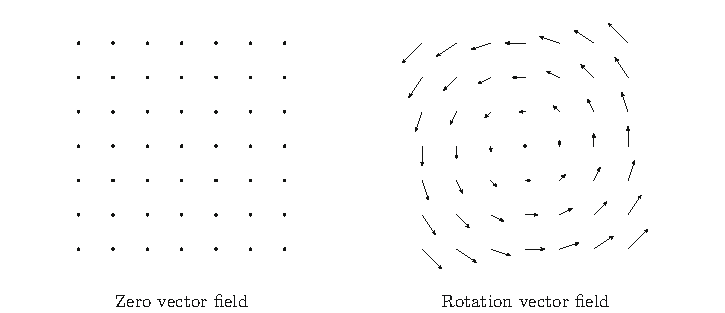
\includegraphics[width=0.92\linewidth]{assets/chapter5/fig5-1.pdf}
\caption{两种保持 $\mathbb R^2$ 上标准高斯分布的向量场：左为零向量场，右为旋转向量场.}\label{fig:5.1}
\end{figure}

为进一步说明这一选择的动机，引入度量空间 $(S,\mathsf d)$ 中曲线 $(x_t)_{t\geq0}$ 的度量导数（metric derivative）. 虽然一般无法赋予一般度量空间中曲线的切向量或“导数”以意义，却可以赋予其速度以意义.

\begin{definition}[度量导数]\label{def:5.2}\index{metric derivative@度量导数（metric derivative）|hyperpage}
设 $(S,\mathsf d)$ 为度量空间，$(x_t)_{t\geq0}$ 为 $S$ 中曲线. 若下列极限存在，则曲线在时刻 $t$ 的度量导数为
$$
|\dot x|(t):=\lim_{s\to t,\ s\ne t}\frac{\mathsf d(x_s,x_t)}{|s-t|}.
$$
\end{definition}

下一个定理表明，这一选择原则产生了良定义的切向量 $v_t$，它有三种刻画方式：(1) 在约束\eqref{eq:5.2}下动能最小的向量场；(2) 满足\eqref{eq:5.2}、且长度 $\|v_t\|_{\mu_t}$ 等于度量导数 $|\dot\mu|(t)$ 的唯一向量场；(3) Brenier 映射的极限.

不过，先引入与 ODE \eqref{eq:5.1}（等价地，与向量场族 $(v_t)_{t\geq0}$）关联的流映射（flow map）. 映射 $F_{0,t}:\mathbb R^d\to\mathbb R^d$ 将给定的 $X_0$ 映为从 $X_0$ 出发的 ODE 在时刻 $t$ 的解 $X_t$. 类似地，对任意两个时刻 $0\leq s\leq t$，可以定义 $F_{s,t}:\mathbb R^d\to\mathbb R^d$. 这个定义的意义在于，将注意力从 ODE 所描述的一条轨迹转向整个空间 $\mathbb R^d$ 在 ODE 作用下的形变.

给定 $\mu,\nu\in\mathcal P_2(\mathbb R^d)$，其中 $\mu$ 有密度，用 $T_{\mu\to\nu}$ 表示从 $\mu$ 到 $\nu$ 的 Brenier 映射，并用 $|\dot\mu|$ 表示 $\mathcal P_2(\mathbb R^d)$ 中曲线相对于度量 $\mathsf d=W_2$ 的度量导数.

\begin{theorem}\label{thm:5.3}
设 $(\mu_t)_{t\geq0}$ 为一条正则的\footnote{这里“正则”可理解为 $\mu_t\in\mathcal P_2(\mathbb R^d)$ 且有密度，并且 $|\dot\mu|(t)$ 对所有 $t\geq0$ 存在. 假设与结论中的“对所有 $t\geq0$”可以替换为“对几乎所有 $t\geq0$”，有密度的假设也可以放宽.}概率测度曲线. 那么，对于满足\eqref{eq:5.2}的每一向量场族 $(v_t)_{t\geq0}$，所有 $t\geq0$ 都有 $|\dot\mu|(t)\leq\|v_t\|_{\mu_t}$.

反之，存在唯一的族 $(v_t)_{t\geq0}$ 满足\eqref{eq:5.2}，并且对每个 $t\geq0$ 有 $|\dot\mu|(t)=\|v_t\|_{\mu_t}$. 这一族满足
\begin{equation}\label{eq:5.5}
v_t=\lim_{h\searrow0}\frac{T_{\mu_t\to\mu_{t+h}}-\mathrm{id}}{h}
\qquad\text{在 }L^2(\mu_t)\text{ 中},
\end{equation}
其中 $\mathrm{id}$ 为恒等函数.
\end{theorem}
\begin{proof}[证明草图]
先证明第一个结论. 设 $(X_t)_{t\geq0}$ 为求解 $\dot X_t=v_t(X_t)$ 的随机变量曲线，且 $X_0\sim\mu_0$. 因为假设连续性方程\eqref{eq:5.2}成立，所以对所有 $t\geq0$ 有 $X_t\sim\mu_t$；特别地，$\mu_{t+h}=(F_{t,t+h})_\#\mu_t$. 利用这个次优耦合可以得到 $W_2(\mu_t,\mu_{t+h})$ 的上界：
$$
\frac{W_2^2(\mu_t,\mu_{t+h})}{h^2}
\leq\mathbb E\left[\frac{\|F_{t,t+h}(X_t)-X_t\|^2}{h^2}\right].
$$
注意 $F_{t,t+h}(X_t)=X_t+hv_t(X_t)+o(h)$，令 $h\to0$，得到 $|\dot\mu|(t)\leq\sqrt{\mathbb E[\|v_t(X_t)\|^2]}=\|v_t\|_{\mu_t}$.

上面的不等式来自采用次优耦合. 直观上，若使 $X_t$ 和 $X_{t+h}$ 最优耦合，并由\eqref{eq:5.5}定义 $v_t$，应当得到等式. 的确如此，但这里省略证明.

最后，结合两项结论可知，若 $(v_t)_{t\geq0}$ 满足\eqref{eq:5.2}且 $|\dot\mu|(t)=\|v_t\|_{\mu_t}$，则
$$
0\in\operatorname*{arg\,min}_{w_t:\mathbb R^d\to\mathbb R^d}\|v_t+w_t\|_{\mu_t}
\quad\text{满足}\quad\operatorname{div}(\mu_tw_t)=0.
$$
而且这是严格凸问题，所以极小化解唯一. 因此，若 $(v_t)_{t\geq0}$ 与 $(u_t)_{t\geq0}$ 均满足连续性方程，且 $\|v_t\|_{\mu_t}=\|u_t\|_{\mu_t}=|\dot\mu|(t)$，则 $w_t=u_t-v_t=0$，得到所述结论.
\end{proof}

上一定理在写出\eqref{eq:5.5}、即断言最优传输映射存在时，使用了 $\mu_t$ 有密度这一事实. 为便于讨论，以下限定在这一测度类上，但将在章末回到粒子方法.

\begin{definition}\label{def:5.4}
$\mathcal P_{2,\mathrm{ac}}(\mathbb R^d)$ 表示 $\mathbb R^d$ 上具有有限二阶矩、且绝对连续（即关于 Lebesgue 测度有密度）的概率测度类.
\end{definition}

\subsection{黎曼几何基础}\label{sec:5.2}

继续之前，先简要、非正式地介绍所需的黎曼几何概念.

流形（manifold）$\mathcal M$ 是局部同胚于欧氏空间 $\mathbb R^d$ 的集合. 在每一点 $p\in\mathcal M$，可以关联一个切空间（tangent space）$T_p\mathcal M$：它是 $d$ 维向量空间，表示经过 $p$ 的曲线所有可能的速度向量. 黎曼度量（Riemannian metric）是在每个切空间上选择一个内积 $\mathfrak g_p$；赋予这一度量后，流形就称为黎曼流形. 为强调其 Hilbert 结构，通常直接用 $\langle\cdot,\cdot\rangle_p$ 表示度量 $\mathfrak g_p$. 为恰当建立微分学理论，一般还要对这些对象施加光滑性假设，但这里侧重于基本语言，不深入细节. 对 Wasserstein 空间，已经为 $\mu_t$ 处的“切向量”（速度场）$v_t$ 找到一个自然范数，即 $L^2$ 范数 $\sqrt{\mathfrak g_{\mu_t}(v_t,v_t)}=\|v_t\|_{\mu_t}$，这提示我们还可以找到黎曼理论的更多 Wasserstein 类比.

下一个重要概念是测地线（geodesic）. 对 $\mathcal M$ 中曲线 $(p_t)_{t\in[0,1]}$，用 $\dot p_t\in T_{p_t}\mathcal M$ 表示时刻 $t$ 的切向量. 给定 $p_0,p_1\in\mathcal M$，二者之间的测地线或最短路径\footnote{在黎曼几何中，通常把测地线定义为仅局部极小化长度的曲线；本书始终用“测地线”指最短路径.}通过求解以下任一变分问题得到：
$$
\min_{(p_t)_{t\in[0,1]}}\int\|\dot p_t\|_{p_t}\,dt
\qquad\text{或}\qquad
\min_{(p_t)_{t\in[0,1]}}\int\|\dot p_t\|_{p_t}^2\,dt,
$$
其中优化范围为连接 $p_0$ 与 $p_1$ 的曲线. 第一个问题的目标泛函是曲线弧长；第二个问题的目标泛函称为能量. 第二种在技术上更方便. 的确，弧长在重新参数化下不变，即对任意连续严格递增函数 $f:[0,1]\to[0,1]$，将 $(p_t)_{t\in[0,1]}$ 换成 $(p_{f(t)})_{t\in[0,1]}$ 不改变弧长，所以第一个问题的解只能在相差重新参数化的意义下唯一. 第二个问题则选出最优曲线的特定参数化，即常速曲线，亦即 $t\mapsto\|\dot p_t\|_{p_t}$ 为常数. 此后只考虑常速测地线，因而省略“常速”这一修饰词.

两变分问题的值分别为 $\mathsf d(p_0,p_1)$ 与 $\mathsf d^2(p_0,p_1)$，其中 $\mathsf d$ 是黎曼度量 $\langle\cdot,\cdot\rangle$ 在 $\mathcal M$ 上诱导的度量空间意义下的度量.

指数映射（exponential map）\footnote{这一名称源于经典流形例子：正交矩阵的集合. 它在单位矩阵处的切空间是反对称矩阵的集合，且指数映射 $\exp_I(A)=\exp(A)$ 就是矩阵指数.}$\exp_p:T_p\mathcal M\to\mathcal M$ 将切向量 $v$ 映为 $p_1$，其中 $(p_t)_{t\in[0,1]}$ 是满足 $p_0=p$、$\dot p_0=v$ 的常速测地线. 其逆映射称为对数映射（logarithmic map）$\log_p:\mathcal M\to T_p\mathcal M$，将 $q$ 映为 $\exp_p^{-1}(q)$. 实际上，指数映射一般未必定义在整个 $T_p\mathcal M$ 上，因为测地线延伸过远后，可能不再是端点间的最短路径；例如，考虑继续延伸球面上从北极到南极的测地线.

有了测地线，就可以定义凸性、梯度和梯度流，它们是曲空间优化的基本构件. 若对所有 $p_0,p_1\in C$ 与 $t\in[0,1]$，都有 $(1-t)p_0+tp_1\in C$，则称 $C\subseteq\mathbb R^d$ 为凸集. 此定义中，$t\mapsto(1-t)p_0+tp_1$ 是连接 $p_0$ 与 $p_1$ 的欧氏测地线. 推广到黎曼流形：若对所有 $p_0,p_1\in C$，连接二者的所有测地线都位于 $C$ 中，则称 $C\subseteq\mathcal M$ 为测地凸\index{Geodesic convexity@测地凸性（Geodesic convexity）|hyperpage}（geodesically convex）集.

还可以定义函数的凸性. 给定 $\alpha\in\mathbb R$，若函数 $f:\mathcal M\to\mathbb R$ 对所有 $t\in[0,1]$ 及所有测地线 $(p_t)_{t\in[0,1]}$ 满足
\begin{equation}\label{eq:5.6}
f(p_t)\leq(1-t)f(p_0)+tf(p_1)-\frac{\alpha t(1-t)}2\mathsf d^2(p_0,p_1),
\end{equation}
则称它为 $\alpha$-测地凸函数. 等价地，有一阶条件
$$
f(q)\geq f(p)+\langle\nabla f(p),\log_p(q)\rangle_p+\frac\alpha2\mathsf d^2(p,q),
\qquad\forall p,q\in\mathcal M,
$$
其中黎曼梯度（Riemannian gradient）$\nabla f$ 定义为：对所有曲线 $(p_t)_{t\geq0}$，$\nabla f(p_t)\in T_{p_t}\mathcal M$ 满足 $\partial_tf(p_t)=\langle\nabla f(p_t),\dot p_t\rangle_{p_t}$. 等价地，还有二阶条件
$$
\nabla^2f(p)[v,v]\geq\alpha\|v\|_p^2,
\qquad\forall p\in\mathcal M,\ \forall v\in T_p\mathcal M,
$$
其中黎曼 Hessian $\nabla^2f$ 可由 $\nabla^2f(p)[v,v]:=\left.\partial_t^2f(p_t)\right|_{t=0}$ 定义，这里 $(p_t)_{t\in[0,1]}$ 为满足 $p_0=p$、$\dot p_0=v$ 的测地线.

下一节回到 $\mathcal P_{2,\mathrm{ac}}(\mathbb R^d)$. 虽然它不是真正的黎曼流形，却具备足够的结构，允许应用黎曼几何的计算法则；事实上，厚重的专著\cite{ref18}就致力于为此建立严格基础. 这产生了一套以 Felix Otto 命名的 Otto 微积分工具，用于研究概率测度空间上的梯度流.

\subsection{Wasserstein 空间的黎曼结构}\label{sec:5.3}

现在可以在 $\mathcal P_2(\mathbb R^d)$ 上定义形式的黎曼结构. 回顾 Brenier 定理（\autoref{thm:1.16}），二次代价的最优传输映射是凸函数的梯度. 由\eqref{eq:5.5}可知，最优速度场位于函数梯度空间的 $L^2$ 闭包中；由于减去了恒等映射，这些函数不一定凸.

\begin{definition}\label{def:5.5}
设 $\mu\in\mathcal P_{2,\mathrm{ac}}(\mathbb R^d)$. 定义 $\mathcal P_{2,\mathrm{ac}}(\mathbb R^d)$ 在 $\mu$ 处的切空间为
$$
T_\mu\mathcal P_{2,\mathrm{ac}}(\mathbb R^d)
:=\overline{\{\nabla\psi\mid\psi:\mathbb R^d\to\mathbb R\text{ 紧支撑且光滑}\}}^{L^2(\mu)},
$$
其中 $\overline{\{\cdot\}}^{L^2(\mu)}$ 表示 $L^2(\mu)$ 闭包. 赋予这一切空间 $L^2(\mu)$ 内积
$$
\langle\nabla\psi_1,\nabla\psi_2\rangle_\mu
:=\int\langle\nabla\psi_1,\nabla\psi_2\rangle\,d\mu.
$$
\end{definition}

可以证明，要求 $v_t$ 为某个函数的梯度 $v_t=\nabla\psi_t$，实际上给出了\autoref{thm:5.3}中最优向量场的第四种刻画，从而为\autoref{def:5.5}提供依据；这里不证明这一点.

\begin{remark}\label{rem:5.6}
稍作停顿，介绍另一种常见约定：不将驱动速度场 $\nabla\psi$ 作为 $\mu_t$ 处的切向量，而采用普通时间导数 $\partial_t\mu_t$，由连续性方程它等于 $\partial_t\mu_t=-\operatorname{div}(\mu_t\nabla\psi)=:\chi$. 此时切空间成为总质量为零的符号测度空间，而度量为 $\langle\chi,\chi'\rangle_\mu=\int\langle\nabla\psi,\nabla\psi'\rangle\,d\mu$，其中 $\psi,\psi'$ 解方程 $\chi=-\operatorname{div}(\mu\nabla\psi)$、$\chi'=-\operatorname{div}(\mu\nabla\psi')$. 这只是记号变化：$\nabla\psi\mapsto\chi$ 是我们所用约定与另一约定之间的等距映射.
\end{remark}

虽然以上逻辑发展强烈暗示了这一黎曼结构与最优传输理论的联系，我们还没有陈述任何相关结果. 下面的定理计算上述度量的常速测地线. 用\autoref{sec:5.2}的语言说，它断言：我们在 $\mathcal P_{2,\mathrm{ac}}(\mathbb R^d)$ 上定义的黎曼结构所诱导的距离，确实就是 Wasserstein 距离.

\begin{theorem}[Benamou--Brenier]\label{thm:5.7}\index{Benamou–Brenier formula@Benamou–Brenier公式（Benamou–Brenier formula）|hyperpage}
设 $\mu_0,\mu_1\in\mathcal P_{2,\mathrm{ac}}(\mathbb R^d)$. 则
\begin{equation}\label{eq:5.7}
W_2^2(\mu_0,\mu_1)=\inf\left\{\int_0^1\|v_t\|_{\mu_t}^2\,dt\ \middle|\
(\mu_t,v_t)_{t\in[0,1]}\text{ 解\eqref{eq:5.2}}\right\}.
\end{equation}
最优曲线 $(\mu_t)_{t\in[0,1]}$ 唯一，描述为 $X_t\sim\mu_t$，其中 $X_t=(1-t)X_0+tX_1$，$(X_0,X_1)\sim\bar\gamma\in\Gamma_{\mu_0,\mu_1}$，而 $\bar\gamma$ 为最优耦合.
\end{theorem}
\begin{proof}
设 $(\mu_t,v_t)_{t\in[0,1]}$ 解\eqref{eq:5.2}，且 $\dot X_t=v_t(X_t)$、$X_0\sim\mu_0$. 于是
$$
\begin{aligned}
W_2^2(\mu_0,\mu_1)
&\leq\mathbb E[\|X_0-X_1\|^2]
=\mathbb E\left[\left\|\int_0^1\dot X_t\,dt\right\|^2\right]\\
&\leq\int_0^1\mathbb E[\|\dot X_t\|^2]\,dt
=\int_0^1\|v_t\|_{\mu_t}^2\,dt.
\end{aligned}
$$
为研究等号情形，注意计算中用了两个不等式. 第一个取等当且仅当 $(X_0,X_1)$ 最优耦合. 第二个取等当且仅当 $t\mapsto\dot X_t$ 为常数，这迫使所有 $t\in[0,1]$ 都有 $\dot X_t=X_1-X_0$.

因此，只需证明存在向量场族 $(v_t)_{t\geq0}$，使所有 $t\in[0,1)$ 都有 $X_1-X_0=v_t((1-t)X_0+tX_1)$. 因为 $(X_0,X_1)$ 最优耦合，存在凸函数 $\varphi$ 满足 $\nabla\varphi(X_0)=X_1$. 于是 $(1-t)X_0+tX_1=\nabla\varphi_t(X_0)$，其中 $\varphi_t(x):=(1-t)\|x\|^2/2+t\varphi(x)$. 特别地，$\varphi_t$ 对所有 $t\in[0,1)$ 强凸，故 $\nabla\varphi_t$ 可逆. 因而可以定义 $v_t:=(\nabla\varphi-\mathrm{id})\circ(\nabla\varphi_t)^{-1}$，满足
$$
\begin{aligned}
v_t((1-t)X_0+tX_1)
&=v_t(\nabla\varphi_t(X_0))\\
&=\nabla\varphi(X_0)-X_0=X_1-X_0,
\end{aligned}
$$
得到所需结论.
\end{proof}

也可以写成 $\mu_t=[(1-t)\mathrm{id}+tT]_\#\mu_0$，其中 $T$ 是从 $\mu_0$ 到 $\mu_1$ 的最优传输映射. 因此给出以下定义.

\begin{definition}\label{def:5.8}
设 $\mu_0,\mu_1\in\mathcal P_{2,\mathrm{ac}}(\mathbb R^d)$，$T$ 为从 $\mu_0$ 到 $\mu_1$ 的最优传输映射. 连接二者的常速测地线为曲线 $(\mu_t)_{t\in[0,1]}$，其中
\begin{equation}\label{eq:5.8}
\mu_t=[(1-t)\mathrm{id}+tT]_\#\mu_0.
\end{equation}
这条曲线称为位移插值（displacement interpolation）、McCann 插值，或简称连接 $\mu_0$ 与 $\mu_1$ 的 Wasserstein 测地线.
\end{definition}

由\eqref{eq:5.8}可以认出 $\log_\mu(\nu)=T_{\mu\to\nu}-\mathrm{id}$，因而 $\exp_\mu(\nabla\psi)=(\mathrm{id}+\nabla\psi)_\#\mu$. 注意，若 $\nabla^2\psi$ 有小于 $-1$ 的特征值，则指数映射没有良好定义，因为这时 $\mathrm{id}+\nabla\psi$ 不是凸函数的梯度，从而不是最优传输映射. 这呼应了此前关于指数映射未必定义在黎曼流形整个切空间上的讨论.\footnote{不过，黎曼流形的指数映射的定义域总包含原点的一个邻域，而 Wasserstein 空间并非如此. 这也是 Wasserstein 空间并非真正的黎曼流形、甚至不是无穷维黎曼流形的原因之一.}

\subsection{Otto 微积分}\label{sec:5.4}

下一步是认出 Wasserstein 梯度，从而定义 Wasserstein 梯度流. 获得泛函测地凸的判别条件之后，就可以得到相应的收敛速率.

Wasserstein 梯度可以用一阶变分表示.

\begin{definition}[一阶变分]\label{def:5.9}\index{first variation@一阶变分（first variation）|hyperpage}
设 $\mathcal F:\mathcal P_{2,\mathrm{ac}}(\mathbb R^d)\to\mathbb R$ 为泛函. $\mathcal F$ 在 $\mu$ 处的一阶变分（first variation），记为 $\delta\mathcal F(\mu):\mathbb R^d\to\mathbb R$，由下式定义：
\begin{equation}\label{eq:5.9}
\lim_{\varepsilon\searrow0}\frac{\mathcal F(\mu+\varepsilon\chi)-\mathcal F(\mu)}{\varepsilon}
=\int\delta\mathcal F(\mu)\,d\chi,
\end{equation}
其中 $\chi$ 遍历满足对充分小的 $\varepsilon$ 都有 $\mu+\varepsilon\chi\in\mathcal P_{2,\mathrm{ac}}(\mathbb R^d)$ 的符号测度.
\end{definition}

若 $(\mu_t)_{t\geq0}$ 为密度曲线，则当 $\varepsilon$ 很小时，可以写线性近似 $\mu_{t+\varepsilon}\approx\mu_t+\varepsilon\partial_t\mu_t$，其中 $\partial_t\mu_t$ 是普通时间导数. 取 $\chi=\partial_t\mu_t$，则\eqref{eq:5.9}成为 $\partial_t\mathcal F(\mu_t)=\int\delta\mathcal F(\mu_t)\,\partial_t\mu_t$. 还应注意，一阶变分只确定到相差一个加法常数，因为扰动 $\chi$ 总满足 $\int d\chi=0$.

现在可以定义 Wasserstein 梯度. 根据定义，给定具有切向量 $(v_t)_{t\geq0}$ 的测度曲线 $(\mu_t)_{t\geq0}$，泛函 $\mathcal F:\mathcal P_{2,\mathrm{ac}}(\mathbb R^d)\to\mathbb R$ 的梯度是 $T_{\mu_t}\mathcal P_{2,\mathrm{ac}}(\mathbb R^d)$ 中满足 $\partial_t\mathcal F(\mu_t)=\langle\nabla\mkern-10mu\nabla\mathcal F(\mu_t),v_t\rangle_{\mu_t}$ 的元素. 下一个命题表明，这一定义可以直接用一阶变分写出.

\begin{proposition}\label{prop:5.10}\index{Wasserstein gradient@Wasserstein梯度（Wasserstein gradient）|hyperpage}
设 $\mathcal F:\mathcal P_{2,\mathrm{ac}}(\mathbb R^d)\to\mathbb R$ 为具有一阶变分 $\delta\mathcal F$ 的泛函. 则 $\mathcal F$ 的 Wasserstein 梯度是向量场 $\nabla\mkern-10mu\nabla\mathcal F(\mu):\mathbb R^d\to\mathbb R^d$，定义为
$$
\nabla\mkern-10mu\nabla\mathcal F(\mu)=\nabla\delta\mathcal F(\mu),
$$
其中右侧的 $\nabla$ 表示普通欧氏梯度.
\end{proposition}
\begin{proof}
设 $(\mu_t)_{t\geq0}$ 为切向量为 $(v_t)_{t\geq0}$ 的测度曲线. $v_t$ 为时刻 $t$ 的切向量，意味着它解连续性方程\eqref{eq:5.2}. 由上面对一阶变分的讨论，
$$
\begin{aligned}
\partial_t\mathcal F(\mu_t)
&=\int\delta\mathcal F(\mu_t)\,\partial_t\mu_t
=-\int\delta\mathcal F(\mu_t)\operatorname{div}(\mu_tv_t)\\
&=\int\langle\nabla\delta\mathcal F(\mu_t),v_t\rangle\,d\mu_t
=\langle\nabla\delta\mathcal F(\mu_t),v_t\rangle_{\mu_t}.
\end{aligned}
$$
而且，$\nabla\delta\mathcal F(\mu_t)$ 为函数的梯度，所以由\autoref{def:5.5}，它属于 $T_{\mu_t}\mathcal P_{2,\mathrm{ac}}(\mathbb R^d)$. 因此，$\nabla\delta\mathcal F(\mu_t)$ 确实是 $\mathcal F$ 在 $\mu_t$ 处的 Wasserstein 梯度.
\end{proof}

因此，计算 Wasserstein 梯度只需先计算一阶变分，再对它取梯度. 用 $\mathcal P_{2,\mathrm{ac}}(\mathbb R^d)$ 上三个典型泛函作说明.

\begin{example}[势能]\label{ex:5.11}\index{potential energy@势能（potential energy）|hyperpage}
设 $\mathcal F(\mu):=\int V\,d\mu$，其中 $V:\mathbb R^d\to\mathbb R$ 为某个势函数（potential）. 那么 $\partial_t\mathcal F(\mu_t)=\int V\,\partial_t\mu_t$，可以认出 $\delta\mathcal F(\mu)=V$，因此 $\nabla\mkern-10mu\nabla\mathcal F(\mu)=\nabla V$.
\end{example}

\begin{example}[内能]\label{ex:5.12}\index{internal energy@内能（internal energy）|hyperpage}
设 $\mathcal F(\mu):=\int U(\mu(x))\,dx$，其中 $U:\mathbb R_+\to\mathbb R$ 为某个函数. 例如，$U(x)=x\log x$ 给出熵泛函.\footnote{这里是热力学熵的负值.}那么 $\partial_t\mathcal F(\mu_t)=\int U'(\mu_t)\,\partial_t\mu_t$，所以 $\delta\mathcal F(\mu)=U'\circ\mu$，从而 $\nabla\mkern-10mu\nabla\mathcal F(\mu)=\nabla(U'\circ\mu)$. 对熵，$\delta\mathcal F(\mu)=\log\mu+1$，且 $\nabla\mkern-10mu\nabla\mathcal F(\mu)=\nabla\log\mu$.
\end{example}

\begin{example}[相互作用能]\label{ex:5.13}\index{interaction energy@相互作用能（interaction energy）|hyperpage}
取对称核 $K:\mathbb R^d\to\mathbb R$，即 $K(-z)=K(z)$. 令 $\mathcal F(\mu):=\frac12\iint K(x-y)\,\mu(dx)\mu(dy)$. 例如，可以考虑高斯核 $K(x)=\exp(-\|x\|^2/(2\sigma^2))$. 那么 $\partial_t\mathcal F(\mu_t)=\iint K(x-y)\,\mu_t(dy)\partial_t\mu_t(dx)$，所以
$$
\delta\mathcal F(\mu)=\int K(\cdot-y)\,\mu(dy),\qquad
\nabla\mkern-10mu\nabla\mathcal F(\mu)=\int\nabla K(\cdot-y)\,\mu(dy).
$$
\end{example}

现在可以定义 $\mathcal P_{2,\mathrm{ac}}(\mathbb R^d)$ 上泛函 $\mathcal F$ 的 Wasserstein 梯度流. 梯度流是时刻 $t$ 的切向量等于 $-\nabla\mkern-10mu\nabla\mathcal F(\mu_t)$ 的测度曲线 $(\mu_t)_{t\geq0}$. 回顾切向量通过连续性方程\eqref{eq:5.2}支配该曲线的演化，得到以下定义.

\begin{definition}[Wasserstein 梯度流]\label{def:5.14}\index{Wasserstein gradient flow@Wasserstein梯度流（Wasserstein gradient flow）|hyperpage}
设 $\mathcal F:\mathcal P_{2,\mathrm{ac}}(\mathbb R^d)\to\mathbb R$ 为泛函. 若 $(\mu_t)_{t\geq0}$ 解偏微分方程
$$
\partial_t\mu_t=\operatorname{div}\bigl(\mu_t\nabla\mkern-10mu\nabla\mathcal F(\mu_t)\bigr),
$$
则称它为 $\mathcal F$ 的 Wasserstein 梯度流（Wasserstein gradient flow）.
\end{definition}

优化理论中早已知道，梯度流是最小化目标泛函 $\mathcal F$ 的自然动力学，因为如下文所述，它总使目标值下降. 因而，Wasserstein 梯度流提供了有原则的方法，用于在概率测度空间上设计最小化某一准则的动力学；这类任务广泛存在于应用数学、统计学及其他领域，见\autoref{sec:6}.

利用 $\mathcal F$ 的 Wasserstein 梯度流 $(\mu_t)_{t\geq0}$ 的定义，简单计算可得
\begin{equation}\label{eq:5.10}
\partial_t\mathcal F(\mu_t)
=\langle\nabla\mkern-10mu\nabla\mathcal F(\mu_t),v_t\rangle_{\mu_t}
=-\|\nabla\mkern-10mu\nabla\mathcal F(\mu_t)\|_{\mu_t}^2,
\end{equation}
其中 $v_t=-\nabla\mkern-10mu\nabla\mathcal F(\mu_t)$ 是时刻 $t$ 的切向量. 此等式表明，目标泛函以等于梯度范数平方的速率耗散，这是梯度流的一般事实. 特别地，若 $\mathcal F$ 有下界，则梯度流的任何极限点都必为 $\mathcal F$ 的驻点.

不过，若能给耗散速率一个定量下界，就能说得更多. 最简单的此类条件是 Polyak\index{Polyak–Łojasiewicz (PŁ) inequality@Polyak–Łojasiewicz（PŁ）不等式（Polyak–Łojasiewicz (PŁ) inequality）|hyperpage}--Łojasiewicz（PŁ）不等式.

\begin{definition}[Polyak--Łojasiewicz（PŁ）不等式]\label{def:5.15}
若对所有 $\mu\in\mathcal P_{2,\mathrm{ac}}(\mathbb R^d)$，都有
$$
\|\nabla\mkern-10mu\nabla\mathcal F(\mu)\|_\mu^2
\geq2\alpha\bigl(\mathcal F(\mu)-\inf\mathcal F\bigr),
$$
则称 $\mathcal F:\mathcal P_{2,\mathrm{ac}}(\mathbb R^d)\to\mathbb R$ 满足常数为 $\alpha>0$ 的 PŁ 不等式.
\end{definition}

$\mathbb R^d$ 上的 PŁ 不等式见\autoref{sec:A.2}；以上定义将它适配至当前情形. 由\eqref{eq:5.10}，PŁ 不等式给出
$$
\partial_t\bigl(\mathcal F(\mu_t)-\inf\mathcal F\bigr)
\leq-2\alpha\bigl(\mathcal F(\mu_t)-\inf\mathcal F\bigr).
$$
令 $\phi(t):=\mathcal F(\mu_t)-\inf\mathcal F$，则 $\dot\phi(t)\leq-2\alpha\phi(t)$. 若这是等式，则可以求解微分方程得到 $\phi(t)=\phi(0)\exp(-2\alpha t)$. 一般地，对于微分不等式，可以用相应微分方程的解控制 $\phi$；这由 Grönwall\index{Grönwall’s inequality@Grönwall不等式（Grönwall’s inequality）|hyperpage} 不等式严格表述.

\begin{lemma}[Grönwall 不等式]\label{lem:5.16}
设 $c\in\mathbb R$，$\phi:[0,T]\to\mathbb R$ 可微，且所有 $t\in[0,T]$ 都满足 $\dot\phi(t)\leq c\phi(t)$. 则
$$
\phi(t)\leq\phi(0)\exp(ct),\qquad\forall t\in[0,T].
$$
\end{lemma}
\begin{proof}
有
$$
\partial_t[\exp(-ct)\phi(t)]
=\exp(-ct)[-c\phi(t)+\dot\phi(t)]\leq0.
$$
所以 $\exp(-ct)\phi(t)\leq\exp(-c\cdot0)\phi(0)=\phi(0)$.
\end{proof}

另一方面，使用与\autoref{lem:A.11}相同的论证，可以证明：只要 $\mathcal F$ 为 $\alpha$-测地凸，就满足常数为 $\alpha$ 的 PŁ 不等式. 得到以下有用的推论.

\begin{corollary}\label{cor:5.17}
设 $\mathcal F:\mathcal P_{2,\mathrm{ac}}(\mathbb R^d)\to\mathbb R$ 为 $\alpha$-测地凸泛函. 则沿着 $\mathcal F$ 的 Wasserstein 梯度流 $(\mu_t)_{t\geq0}$，有
$$
\mathcal F(\mu_t)-\inf\mathcal F
\leq e^{-2\alpha t}\bigl(\mathcal F(\mu_0)-\inf\mathcal F\bigr).
$$
\end{corollary}

\subsection{Bures--Wasserstein 几何}\label{sec:5.5}\index{Bures–Wasserstein@Bures–Wasserstein|hyperpage}

将上一节的概念应用于 Wasserstein 空间中由高斯测度组成的子流形，很有启发性.

\begin{definition}\label{def:5.18}
Bures--Wasserstein 空间（Bures--Wasserstein space）$\mathsf{BW}(\mathbb R^d)$ 是赋予 Wasserstein 度量的 $\mathbb R^d$ 上非退化高斯分布的空间.
\end{definition}

具体地，因为高斯分布由均值与协方差矩阵参数化，可以将 $\mathsf{BW}(\mathbb R^d)$ 视为 $\mathbb R^d\times\mathbb S_{++}^d$，其中 $\mathbb S_{++}^d$ 是对称正定 $d\times d$ 矩阵的锥. 回顾\autoref{ex:1.19}，对任意 $\mu_0,\mu_1\in\mathsf{BW}(\mathbb R^d)$，从 $\mu_0$ 到 $\mu_1$ 的最优传输映射 $T$ 为仿射映射，而连接二者的 Wasserstein 测地线为
$$
\mu_t=[\underbrace{(1-t)\mathrm{id}+tT}_{\text{仿射映射}}]_\#\mu_0,
\qquad t\in[0,1].
$$
因为非退化高斯分布经非奇异仿射映射的推前仍为非退化高斯分布，所以这条测地线完全位于 $\mathsf{BW}(\mathbb R^d)$ 内. 换言之：

\begin{proposition}\label{prop:5.19}
$\mathsf{BW}(\mathbb R^d)\subseteq\mathcal P_{2,\mathrm{ac}}(\mathbb R^d)$ 为测地凸集.
\end{proposition}

回顾黎曼流形 $\mathcal M$ 上的泛函 $\mathcal F$：若对 $\mathcal M$ 上所有测地线 $(p_t)_{t\in[0,1]}$，映射 $[0,1]\to\mathcal M$、$t\mapsto\mathcal F(p_t)$ 都为 $\alpha$-凸的，则称 $\mathcal F$ 为 $\alpha$-测地凸的. $\mathsf{BW}(\mathbb R^d)$ 的测地凸性意味着，其内蕴测地线与 Wasserstein 测地线重合，立即得到以下推论.

\begin{corollary}\label{cor:5.20}
设 $\mathcal F:\mathcal P_{2,\mathrm{ac}}(\mathbb R^d)\to\mathbb R$ 为 $\alpha$-测地凸泛函. 那么，将它视为 $\mathsf{BW}(\mathbb R^d)$ 上的泛函时，仍为 $\alpha$-测地凸的.
\end{corollary}

\autoref{sec:6.1.2}将用到这一事实.

$\mathcal P_{2,\mathrm{ac}}(\mathbb R^d)$ 的黎曼结构下降到 $\mathsf{BW}(\mathbb R^d)$，使 Bures--Wasserstein 空间具有真正的有限维黎曼流形结构. 在 $\mu\in\mathsf{BW}(\mathbb R^d)$ 处的切空间为
$$
\begin{aligned}
T_\mu\mathsf{BW}(\mathbb R^d)
&=\{\lambda(T_{\mu\to\nu}-\mathrm{id})\mid\lambda>0,\ \nu\in\mathsf{BW}(\mathbb R^d)\}\\
&=\{x\mapsto Sx+a\mid a\in\mathbb R^d,\ S\in\mathbb S^d\},
\end{aligned}
$$
其中 $\mathbb S^d$ 为对称 $d\times d$ 矩阵空间. 实际上，将切空间重新参数化为
$$
T_\mu\mathsf{BW}(\mathbb R^d)
=\{x\mapsto S(x-m)+a\mid a\in\mathbb R^d,\ S\in\mathbb S^d\}
$$
更方便，其中 $m=\mathbb E_{X\sim\mu}[X]$.

根据定义，$\mathsf{BW}(\mathbb R^d)$ 上诱导的黎曼结构，是将 $T_\mu\mathcal P_{2,\mathrm{ac}}(\mathbb R^d)$ 上的内积限制到子空间 $T_\mu\mathsf{BW}(\mathbb R^d)$，即 $L^2(\mu)$ 内积. 据此，可以从头计算泛函 $\mathcal F$ 的 BW 梯度. 不过，我们已经算出 $\mathcal F$ 在 $\mu$ 处的 Wasserstein 梯度为向量场 $\nabla\mkern-10mu\nabla\mathcal F(\mu)=\nabla\delta\mathcal F(\mu)$（\autoref{prop:5.10}），因此更快捷的方法是将它正交投影到 $T_\mu\mathsf{BW}(\mathbb R^d)$.

\begin{theorem}\label{thm:5.21}\index{Bures–Wasserstein@Bures–Wasserstein!gradient@梯度（gradient）|hyperpage}
设泛函 $\mathcal F:\mathcal P_{2,\mathrm{ac}}(\mathbb R^d)\to\mathbb R$ 在 $\mu$ 处具有一阶变分 $\delta\mathcal F(\mu)$. 那么，$\mathcal F$ 在 $\mu\in\mathsf{BW}(\mathbb R^d)$ 处的 Bures--Wasserstein 梯度为仿射映射
$$
x\mapsto\left(\int\nabla^2\delta\mathcal F(\mu)\,d\mu\right)(x-m)
+\int\nabla\delta\mathcal F(\mu)\,d\mu,
$$
其中 $m=\int x\,\mu(dx)$ 为 $\mu$ 的均值.
\end{theorem}
\begin{proof}
回顾 $\nabla\mkern-10mu\nabla\mathcal F(\mu)=\nabla\delta\mathcal F(\mu)$（\autoref{prop:5.10}）. 在 $\mu$ 处的 BW 梯度为 $\nabla\delta\mathcal F(\mu)$ 在 $T_\mu\mathsf{BW}(\mathbb R^d)$ 上的正交投影；根据定义，它是满足下式的元素 $\nabla_{\mathsf{BW}}\mathcal F(\mu)\in T_\mu\mathsf{BW}(\mathbb R^d)$：
\begin{equation}\label{eq:5.11}
\langle\nabla_{\mathsf{BW}}\mathcal F(\mu),v\rangle_\mu
=\langle\nabla\delta\mathcal F(\mu),v\rangle_\mu,
\qquad\forall v\in T_\mu\mathsf{BW}(\mathbb R^d).
\end{equation}
可以更显式地写出这一条件. 因为 $\nabla_{\mathsf{BW}}\mathcal F(\mu)$ 与 $v$ 都在该切空间中，它们具有形式
$$
\begin{aligned}
\nabla_{\mathsf{BW}}\mathcal F(\mu)&=S(\cdot-m)+a,\\
v&=\widetilde S(\cdot-m)+\widetilde a.
\end{aligned}
$$
一方面，
\begin{equation}\label{eq:5.12}
\begin{aligned}
\langle\nabla_{\mathsf{BW}}\mathcal F(\mu),v\rangle_\mu
&=\mathbb E_{X\sim\mu}\langle S(X-m)+a,\widetilde S(X-m)+\widetilde a\rangle\\
&=\langle S,\Sigma\widetilde S\rangle+\langle a,\widetilde a\rangle,
\end{aligned}
\end{equation}
其中 $\Sigma$ 为 $\mu$ 的协方差矩阵. 另一方面，
\begin{align}
\langle\nabla\delta\mathcal F(\mu),v\rangle_\mu
&=\mathbb E_{X\sim\mu}\langle[\nabla\delta\mathcal F(\mu)](X),\widetilde S(X-m)+\widetilde a\rangle\nonumber\\
&=\langle\mathbb E_{X\sim\mu}[\nabla\delta\mathcal F(\mu)(X)(X-m)^{\mathsf T}],\widetilde S\rangle\label{eq:5.13}\\
&\qquad+\langle\mathbb E_{X\sim\mu}\nabla\delta\mathcal F(\mu)(X),\widetilde a\rangle.\label{eq:5.14}
\end{align}
另外，分部积分给出
$$
\begin{aligned}
&\mathbb E_{X\sim\mu}[\nabla\delta\mathcal F(\mu)(X)(X-m)^{\mathsf T}]\\
&\quad=\int\nabla\delta\mathcal F(\mu)\bigl(\Sigma\Sigma^{-1}(\cdot-m)\bigr)^{\mathsf T}\,d\mu\\
&\quad=-\int\nabla\delta\mathcal F(\mu)(\nabla\log\mu)^{\mathsf T}\,d\mu\,\Sigma\\
&\quad=-\int\nabla\delta\mathcal F(\mu)(\nabla\mu)^{\mathsf T}\,\Sigma\\
&\quad=\int\nabla^2\delta\mathcal F(\mu)\,d\mu\,\Sigma.
\end{aligned}
$$
所以
\begin{equation}\label{eq:5.15}
\begin{aligned}
&\langle\mathbb E_{X\sim\mu}[\nabla\delta\mathcal F(\mu)(X)(X-m)^{\mathsf T}],\widetilde S\rangle\\
&\quad=\left\langle\int\nabla^2\delta\mathcal F(\mu)\,d\mu\,\Sigma,\widetilde S\right\rangle\\
&\quad=\left\langle\Sigma\int\nabla^2\delta\mathcal F(\mu)\,d\mu,\widetilde S\right\rangle\\
&\quad=\left\langle\int\nabla^2\delta\mathcal F(\mu)\,d\mu,\Sigma\widetilde S\right\rangle.
\end{aligned}
\end{equation}
因为\eqref{eq:5.11}应对所有 $\widetilde a\in\mathbb R^d$ 和 $\widetilde S\in\mathbb S^d$ 成立，比较\eqref{eq:5.12}、\eqref{eq:5.13}、\eqref{eq:5.14}及\eqref{eq:5.15}，得到
$$
S=\int\nabla^2\delta\mathcal F(\mu)\,d\mu,
\qquad a=\int\nabla\delta\mathcal F(\mu)\,d\mu.
$$
推导完成.
\end{proof}

认出 BW 梯度后，可以用连续性方程的 Lagrange 解释，通过以下动力学实现梯度流：
$$
\begin{aligned}
\dot X_t&=-\nabla_{\mathsf{BW}}\mathcal F(\mu_t)(X_t)\\
&=-\left(\int\nabla^2\delta\mathcal F(\mu_t)\,d\mu_t\right)(X_t-m_t)
-\int\nabla\delta\mathcal F(\mu_t)\,d\mu_t,
\end{aligned}
$$
其中 $X_t\sim\mu_t$，分别用 $m_t$ 与 $\Sigma_t$ 表示 $\mu_t$ 的均值与协方差. 不过，$\mu_t$ 在每个 $t\geq0$ 都是高斯分布，因此直接通过 $m_t$、$\Sigma_t$ 精确追踪 $\mu_t$ 更方便. 它们遵循动力学
$$
\dot m_t=\mathbb E\dot X_t=-\int\nabla\delta\mathcal F(\mu_t)\,d\mu_t,
$$
以及
$$
\begin{aligned}
\dot\Sigma_t
&=\partial_t\mathbb E[(X_t-m_t)(X_t-m_t)^{\mathsf T}]\\
&=\mathbb E[\dot X_t(X_t-m_t)^{\mathsf T}]
+\mathbb E[(X_t-m_t)\dot X_t^{\mathsf T}]\\
&=-\mathbb E\Biggl[\Biggl(\left(\int\nabla^2\delta\mathcal F(\mu_t)\,d\mu_t\right)(X_t-m_t)\\
&\hspace{5em}+\int\nabla\delta\mathcal F(\mu_t)\,d\mu_t\Biggr)(X_t-m_t)^{\mathsf T}\Biggr]+\cdots\\
&=-\left(\int\nabla^2\delta\mathcal F(\mu_t)\,d\mu_t\right)
\mathbb E[(X_t-m_t)(X_t-m_t)^{\mathsf T}]+\cdots\\
&=-\left(\int\nabla^2\delta\mathcal F(\mu_t)\,d\mu_t\right)\Sigma_t
-\Sigma_t\left(\int\nabla^2\delta\mathcal F(\mu_t)\,d\mu_t\right),
\end{aligned}
$$
其中 $A+\cdots$ 是 $A+A^{\mathsf T}$ 的简写. 终于得到显式的方程组.

\begin{theorem}\label{thm:5.22}
泛函 $\mathcal F$ 的 BW 梯度流为曲线 $(\mu_t=\mathcal N(m_t,\Sigma_t))_{t\geq0}$，其中
\begin{equation}\label{eq:5.16}
\begin{aligned}
\dot m_t&=-\mathbb E\nabla\delta\mathcal F(\mu_t)(X_t),\\
\dot\Sigma_t&=-\mathbb E\nabla^2\delta\mathcal F(\mu_t)(X_t)\,\Sigma_t
-\Sigma_t\mathbb E\nabla^2\delta\mathcal F(\mu_t)(X_t),
\end{aligned}
\end{equation}
且 $X_t\sim\mu_t$.
\end{theorem}

\subsection{高斯混合}\label{sec:5.6}

在\autoref{sec:5.5}的思想之上，现在考虑丰富得多的高斯混合空间上的梯度流. 事实上，如下文所解释的，换一种恰当视角，$\mathbb R^d$ 上任意测度都可以视为高斯混合.

在此之前，先指出：类似于\autoref{sec:5.5}的做法，直接将 Wasserstein 梯度流限制在高斯混合空间上，是行不通的. 问题在于，无法显式计算两个高斯混合之间的最优传输映射，即便在无穷小层面也不行，所以无法认出切空间；除非每个高斯混合只有一个分量，或只有一维. 不过，根据\cite{ref69,ref107}，可以考虑一种自然的几何结构：Bures--Wasserstein 之上的 Wasserstein 几何.

通常将高斯混合介绍为形如 $\sum_{k=1}^Kw_k\mathcal N(m_k,\Sigma_k)$ 的分布，其中混合权重 $w_k\geq0$、$\sum_{k=1}^Kw_k=1$；但可以更广泛地将高斯混合定义为形如 $\int\mathcal N(m,\Sigma)\,\nu(dm,d\Sigma)$ 的测度. 上述有限高斯混合对应于离散混合测度（mixing measure）$\nu=\sum_{k=1}^Kw_k\delta_{(m_k,\Sigma_k)}$. 这个更广泛的新定义本身几乎没有用，因为任意测度 $\mu$ 都可以如此表示：$\mu=\int\delta_x\,\mu(dx)$，其中 $\delta_x=\mathcal N(x,0)$ 为退化高斯分布. 而且，用混合测度 $\nu$ 表示高斯混合是“过参数化”的，即 $\nu$ 极不唯一：考虑等式 $\mathcal N(0,I)=\int\mathcal N(x,\tau I)\,\nu(dx)$，其中 $\nu=\mathcal N(0,(1-\tau)I)$，它对任意 $\tau\in[0,1]$ 都成立. 尽管如此，这一视角有用之处在于，它给出自然解释：高斯混合的混合测度就是 Bures--Wasserstein 空间上的概率测度. 下面看这如何引出几何结构的定义.

Bures--Wasserstein 空间是黎曼流形. 如前所述，赋予某种黎曼度量的流形 $\mathbb R^d\times\mathbb S_{++}^d$ 与空间 $\mathsf{BW}(\mathbb R^d)$ 等距. 以下考虑由 Otto 微积分产生的度量，但这里也可以采用任意其他度量，包括欧氏度量.

也可在任意度量空间上考虑有限二阶矩的概率测度空间，并赋予它 $2$-Wasserstein 距离. 的确，回顾\autoref{sec:1.1}，最优传输问题可以用更一般的代价定义，所以可以取度量空间上的距离平方作为代价.

当该度量空间为黎曼流形时，适当修改后，\autoref{sec:5.1}至\autoref{sec:5.4}的结果仍然成立. 这里不作详细论证，但建议读者从新的视角重读这些节. 例如 ODE \eqref{eq:5.1}仍有意义，只要记住流形 $\mathcal M$ 上的向量场 $v$，是给每一点 $x\in\mathcal M$ 指定切向量 $v(x)\in T_x\mathcal M$ 的映射 $x\mapsto v(x)$. 连续性方程的弱形式\eqref{eq:5.3}也仍有意义，其中 $\nabla$ 现在指黎曼梯度；若将 $\mu_t$ 解释为关于体积测度的密度，甚至\eqref{eq:5.2}也有意义，等等. 事实上，这一几何背景是最优传输理论中一些最深刻进展的源头，见\cite{ref317}.

对我们而言，关键在于\autoref{prop:5.10}给出的 Wasserstein 梯度公式仍然成立，同样将 $\nabla$ 解释为黎曼梯度.

综合上述讨论，可以推导出位于空间 $(\mathcal P_2(\mathsf{BW}(\mathbb R^d)),W_2)$ 中的 Wasserstein 梯度流.

\begin{theorem}\label{thm:5.23}
给定 $\nu\in\mathcal P_2(\mathsf{BW}(\mathbb R^d))$，用 $G_\nu$ 表示相应的高斯混合
$$G_\nu=\int\mathcal N(m,\Sigma)\,\nu(dm,d\Sigma).$$
设 $\mathcal F$ 为 $\mathcal P_2(\mathbb R^d)$ 上的泛函，$\mathcal G$ 为 $\mathcal P_2(\mathsf{BW}(\mathbb R^d))$ 上由 $\nu\mapsto\mathcal F(G_\nu)$ 给出的对应泛函. 那么，$\mathcal G$ 的 Wasserstein 梯度流为如下曲线 $(\nu_t)_{t\geq0}$：$\nu_t=\operatorname{law}(m_t,\Sigma_t)$，其中
$$
\begin{aligned}
\dot m_t&=-\mathbb E\nabla\delta\mathcal F(G_{\nu_t})(X_t),\\
\dot\Sigma_t&=-\mathbb E\nabla^2\delta\mathcal F(G_{\nu_t})(X_t)\,\Sigma_t
-\Sigma_t\mathbb E\nabla^2\delta\mathcal F(G_{\nu_t})(X_t),
\end{aligned}
$$
且 $X_t\sim\mathcal N(m_t,\Sigma_t)$.
\end{theorem}
\begin{proof}
$\mathcal G$ 的一阶变分如下计算. 若 $(\nu_t)_{t\in\mathbb R}$ 是 $\mathcal P_2(\mathsf{BW}(\mathbb R^d))$ 中的曲线，则
$$\partial_tG_{\nu_t}=\int\mathcal N(m,\Sigma)\,\partial_t\nu_t(dm,d\Sigma).$$
因此
$$
\begin{aligned}
\partial_t\mathcal G(\nu_t)
&=\partial_t\mathcal F(G_{\nu_t})
=\int\delta\mathcal F(G_{\nu_t})\,\partial_tG_{\nu_t}\\
&=\iint\delta\mathcal F(G_{\nu_t})\,d\mathcal N(m,\Sigma)\,\partial_t\nu_t(dm,d\Sigma).
\end{aligned}
$$
所以一阶变分为
$$
\delta\mathcal G(\nu):(m,\Sigma)\mapsto\int\delta\mathcal F(G_\nu)\,d\mathcal N(m,\Sigma).
$$
根据 $\mathsf{BW}(\mathbb R^d)$ 与 $\mathbb R^d\times\mathbb S_{++}^d$ 的对应，$\delta\mathcal G(\nu)$ 在 $(m,\Sigma)$ 处的黎曼梯度，与泛函 $\mu\mapsto\int\delta\mathcal F(G_\nu)\,d\mu$ 在 $\mu=\mathcal N(m,\Sigma)$ 处的 Bures--Wasserstein 梯度相同，而后者已在\autoref{thm:5.21}中计算. 因此结论由\autoref{thm:5.22}得到.
\end{proof}

\subsection{Wasserstein--Fisher--Rao 几何}\label{sec:5.7}

现在描述 Wasserstein 几何的一种变体，它在应用中经常有用，\autoref{sec:6}将予以说明. 这一变体称为 Wasserstein--Fisher--Rao（WFR）或 Hellinger--Kantorovich 距离，最初作为非平衡\index{unbalanced optimal transport@非平衡最优传输（unbalanced optimal transport）|hyperpage}最优传输（unbalanced optimal transport）的模型提出并研究，即总质量未必相同的正测度之间的最优传输. 一个显著例子是前言提到的细胞轨迹重建：用测度表示不同时刻的细胞群体快照，而细胞的出生与死亡确实会改变总质量.

从静态视角看，WFR 定义了最优传输问题的一种变体，可以类似\autoref{sec:1}那样研究其代价、度量性质、对偶等. 这一方向的详细研究见\cite{ref84,ref183,ref209,ref210}. 本节遵循\cite[附录 H]{ref192}，侧重于所得度量空间的黎曼结构，以推导梯度流.

\subsubsection*{Fisher--Rao}
讨论 Wasserstein--Fisher--Rao 之前，先介绍其关键组成之一：Fisher--Rao 度量. 这是 $\mathbb R^d$ 上正测度空间 $\mathcal M_+(\mathbb R^d)$ 上的度量，定义为
$$
\mathsf d_{\mathsf{FR}}^2(\mu_0,\mu_1):=\int(\sqrt{\mu_0}-\sqrt{\mu_1})^2,
$$
其中照常将测度与其 Lebesgue 密度等同，并假设密度存在.\footnote{密度不存在时，可以对任意共同控制测度 $\lambda$ 定义 $\mathsf d_{\mathsf{FR}}^2(\mu_0,\mu_1):=\int(\sqrt{d\mu_0/d\lambda}-\sqrt{d\mu_1/d\lambda})^2\,d\lambda$.}当 $\mu_0,\mu_1$ 为概率测度时，$\mathsf d_{\mathsf{FR}}$ 就是统计学中的 Hellinger 距离.\footnote{这解释了 WFR 度量并存的命名约定；注意 $\{\text{Wasserstein},\text{Fisher--Rao}\}\cong\{\text{Hellinger},\text{Kantorovich}\}$.}

几何上，$\mathsf d_{\mathsf{FR}}$ 是通过要求 $\mu\mapsto\sqrt\mu$ 等距嵌入 Hilbert 空间 $L^2(\mathbb R^d)$ 而得到的非负密度上的度量. 因而 $(\mathcal M_+(\mathbb R^d),\mathsf d_{\mathsf{FR}})$ 的几何是平坦的，可以通过该等距映射得到黎曼结构. 具体地，若 $\dot\mu$ 表示密度曲线的时间导数，则平方根的导数为 $\dot{\sqrt\mu}=\dot\mu/(2\sqrt\mu)$. 若用 $L^2(\mathbb R^d)$ 范数衡量后者的“长度”，得到切空间 $T_\mu\mathcal M_+(\mathbb R^d)$ 上的诱导黎曼度量
$$
\mathfrak g_\mu(\dot\mu,\dot\mu)
:=\|\dot{\sqrt\mu}\|_{L^2(\mathbb R^d)}^2=\int\frac{\dot\mu^2}{4\mu},
$$
该切空间由函数 $\dot\mu:\mathbb R^d\to\mathbb R$ 组成.

这一几何建立在所有正测度的空间上，包括质量总量不同的测度，因而适合刻画自然发生质量变化的物理情形. 典型例子是 $\mu$ 表示化学物质浓度，而浓度随化学反应变化. 这由反应方程（reaction equation）$\partial_t\mu_t=\alpha_t\mu_t$ 建模，其中 $\alpha_t:\mathbb R^d\to\mathbb R$ 规定每个空间点的反应速率. 此记号中 $\alpha=\dot\mu/\mu$，相当于对切空间重新参数化. 换言之，也可以将切空间视为函数 $\alpha:\mathbb R^d\to\mathbb R$ 构成的空间，并赋予度量
\begin{equation}\label{eq:5.17}\index{Fisher–Rao@Fisher–Rao|hyperpage}
\widetilde{\mathfrak g}_\mu(\alpha,\alpha)
:=\mathfrak g_\mu(\alpha\mu,\alpha\mu)=\frac14\int\alpha^2\,d\mu.
\end{equation}
以下采用这一定义，因而记 $\|\alpha\|_\mu^2:=\widetilde{\mathfrak g}_\mu(\alpha,\alpha)$.

与 Wasserstein 几何的定义比较：在每个测度 $\mu$ 处，“切空间”$T_\mu\mathcal M_+(\mathbb R^d)$ 现在定义为所有函数 $\alpha:\mathbb R^d\to\mathbb R$ 的空间，赋予度量\eqref{eq:5.17}，并用反应方程 $\partial_t\mu_t=\alpha_t\mu_t$ 取代连续性方程. 与 Wasserstein 度量相比，Fisher--Rao 度量基于完全不同的直觉：反应方程描述质量的自发产生与消灭，而非质量传输.

虽然 Fisher--Rao 几何的动机涉及质量变化，我们也可能希望将它用于需要始终在概率测度空间上流动的问题. 为此，考虑 $\mathcal P(\mathbb R^d)$ 上的诱导几何. 方程 $\partial_t\mu_t=\alpha_t\mu_t$ 保持总质量不变，当且仅当所有 $t\geq0$ 都有 $\int\alpha_t\,d\mu_t=0$，所以将切空间限制为 $T_\mu\mathcal P(\mathbb R^d)=\{\alpha:\mathbb R^d\to\mathbb R\mid\int\alpha\,d\mu=0\}$，并赋予度量\eqref{eq:5.17}.\footnote{一个离散类比是：给 $\{1,\ldots,d\}$ 上概率测度的空间，即 $\mathbb R^d$ 中的单纯形，通过等距映射 $p\mapsto\sqrt p$ 赋予几何，其中 $\sqrt p$ 是单位球面 $S^{d-1}$ 的元素. 见\autoref{exer:5.13}.}质量守恒保证，任意被消灭的质量都会在别处立即产生. 沿用传输的语言，这种现象有时称为瞬移（teleportation）；不过，它仅仅对应于重新加权.

梯度流又如何？给定泛函 $\mathcal F:\mathcal M_+(\mathbb R^d)\to\mathbb R$ 或 $\mathcal F:\mathcal P(\mathbb R^d)\to\mathbb R$，根据定义，沿着任意满足 $\partial_t\mu_t=\alpha_t\mu_t$ 的曲线，梯度满足 $\partial_t\mathcal F(\mu_t)=\langle\nabla_{\mathsf{FR}}\mathcal F(\mu_t),\alpha_t\rangle_{\mu_t}$. 展开定义可以验证（见\autoref{exer:5.14}）
\begin{equation}\label{eq:5.18}
\begin{aligned}
\nabla_{\mathsf{FR}}\mathcal F(\mu)&=\delta\mathcal F(\mu),\qquad\text{或}\\
\nabla_{\mathsf{FR}}\mathcal F(\mu)&=\delta\mathcal F(\mu)-\int\delta\mathcal F(\mu)\,d\mu,
\end{aligned}
\end{equation}
分别对应于 $\mathcal M_+(\mathbb R^d)$ 和 $\mathcal P(\mathbb R^d)$；这里 $\delta\mathcal F$ 为一阶变分（\autoref{def:5.9}）. 为区分两种情况并强调 WFR 度量来自非平衡最优传输的初衷，将前者称为非平衡 Fisher--Rao，后者简称 Fisher--Rao. $\mathcal F$ 的 Fisher--Rao 梯度流在时刻 $t$ 沿切向量 $-\nabla_{\mathsf{FR}}\mathcal F(\mu_t)$ 演化，满足
\begin{equation}\label{eq:5.19}
\partial_t\mu_t=-\nabla_{\mathsf{FR}}\mathcal F(\mu_t)\,\mu_t.
\end{equation}

\subsubsection*{Wasserstein--Fisher--Rao}
现在将 Wasserstein 与 Fisher--Rao 两种几何结合，得到同时包含质量传输及产生／消灭（也称重新加权或瞬移）的混合几何. 方法是直接考虑带反应的连续性方程 $\partial_t\mu_t+\operatorname{div}(\mu_tv_t)=\alpha_t\mu_t$. 支配方程由函数 $\alpha$ 和向量场 $v$ 参数化，两者共同构成切向量. 因而自然考虑度量\footnote{严格说，将 Wasserstein 与 Fisher--Rao 几何相加时，应在 $\alpha^2$ 项前加系数 $1/4$；部分文献确实采用这一约定. 为简洁起见，本书省略该系数.}
\begin{equation}\label{eq:5.20}\index{Wasserstein–Fisher–Rao (WFR)@Wasserstein–Fisher–Rao（WFR）（Wasserstein–Fisher–Rao (WFR)）|hyperpage}
\|(\alpha,v)\|_\mu^2=\int(\alpha^2+\|v\|^2)\,d\mu.
\end{equation}
不过，与\autoref{sec:5.1}的讨论类似，这尚未唯一确定切向量，因为在保持同一测度演化 $(\mu_t)_{t\geq0}$ 的同时，$(\alpha,v)$ 的选择仍有过多自由. 可以证明，使范数\eqref{eq:5.20}最小的最优对 $(\alpha,v)$（参见\autoref{sec:5.1}）可刻画为：对某个函数 $\psi:\mathbb R^d\to\mathbb R$，$\alpha=\psi$、$v=\nabla\psi$. 因而，可以将 $\mu$ 处的 WFR 切空间定义为
$$
T_\mu\mathcal M_+(\mathbb R^d)
=\overline{\{(\psi,\nabla\psi)\mid\psi:\mathbb R^d\to\mathbb R\text{ 紧支撑且光滑}\}}^{L^2(\mu)},
$$
并赋予范数
\begin{equation}\label{eq:5.21}
\|(\psi,\nabla\psi)\|_\mu^2:=\int(\psi^2+\|\nabla\psi\|^2)\,d\mu.
\end{equation}
它有一种令人满意的解释：将 Wasserstein 度量 $\|\nabla\psi\|_{L^2(\mu)}^2$ “补全”为 $\psi$ 的完整 Sobolev 范数. 还应注意，支配方程成为
\begin{equation}\label{eq:5.22}
\partial_t\mu_t+\operatorname{div}(\mu_t\nabla\psi_t)=\psi_t\mu_t.
\end{equation}
与之前一样，也可以限制到概率测度空间 $\mathcal P(\mathbb R^d)$，此时只考虑满足 $\int\psi\,d\mu=0$ 的对 $(\psi,\nabla\psi)$，并赋予同一度量\eqref{eq:5.21}. 称整个空间 $\mathcal M_+(\mathbb R^d)$ 上的 WFR 为非平衡 WFR，以下将 WFR 专指其在 $\mathcal P(\mathbb R^d)$ 上的限制.

下一个定理计算 WFR 梯度.

\begin{theorem}\label{thm:5.24}
设 $\mathcal F$ 为 $\mathcal M_+(\mathbb R^d)$ 或 $\mathcal P(\mathbb R^d)$ 上的泛函. 那么，$\mathcal F$ 的非平衡 WFR 梯度记为 $\nabla\mkern-10mu\nabla_{\mathsf{FR}}\mathcal F$，满足
$$
\nabla\mkern-10mu\nabla_{\mathsf{FR}}\mathcal F(\mu)
=\bigl(\delta\mathcal F(\mu),\nabla\delta\mathcal F(\mu)\bigr),
$$
而 WFR 梯度为
$$
\nabla\mkern-10mu\nabla_{\mathsf{FR}}\mathcal F(\mu)
=\left(\delta\mathcal F(\mu)-\int\delta\mathcal F(\mu)\,d\mu,\nabla\delta\mathcal F(\mu)\right).
$$
\end{theorem}
\begin{proof}
设 $(\mu_t)_{t\geq0}$ 满足\eqref{eq:5.22}. 分部积分给出
$$
\partial_t\mathcal F(\mu_t)
=\int\langle\nabla\delta\mathcal F(\mu_t),\nabla\psi_t\rangle\,d\mu_t
+\int\delta\mathcal F(\mu_t)\psi_t\,d\mu_t.
$$
在非平衡情形，根据度量\eqref{eq:5.21}的定义，可以将它认作
$$
\langle(\delta\mathcal F(\mu),\nabla\delta\mathcal F(\mu)),(\psi_t,\nabla\psi_t)\rangle_{\mu_t}.
$$
在平衡情形，有 $\int\psi_t\,d\mu_t=0$；而且 WFR 梯度按定义属于切空间，其第一分量也必须均值为零，故结论成立.
\end{proof}

因此 WFR 梯度流为
\begin{equation}\label{eq:5.23}
\partial_t\mu_t=\operatorname{div}\bigl(\mu_t\nabla\delta\mathcal F(\mu_t)\bigr)
-\left(\delta\mathcal F(\mu_t)-\int\delta\mathcal F(\mu_t)\,d\mu_t\right)\mu_t.
\end{equation}

\subsection{平均场粒子系统}\label{sec:5.8}

本章最后从粒子系统（particle system）的视角描述 Wasserstein 和 WFR 梯度流. 当这些梯度流从有限测度出发时，粒子系统自然出现. 的确，一个关键观察是：两种梯度流都可以用常微分方程实现，所以若 $\mu_0$ 为有限测度，则沿这些梯度流，$\mu_t$ 在所有时刻 $t$ 都仍是有限测度.

\subsubsection{粒子 Wasserstein 梯度流}\label{sec:5.8.1}

为说明这一点，设 $\mathcal F$ 为 $\mathcal P(\mathbb R^d)$ 上的函数，并回顾\autoref{def:5.14}：$\mathcal F$ 的 Wasserstein 梯度流是与 ODE
\begin{equation}\label{eq:5.24}
\dot X_t=-\nabla\mkern-10mu\nabla\mathcal F(\mu_t)(X_t)
\end{equation}
关联的连续性方程，其中 $\mu_t$ 表示 $X_t$ 的分布. 特别地，只需在 $\mu_t$ 的支撑上描述这些动力学.

现在假设 Wasserstein 梯度流的初值为
$$
\mu_0:=\frac1N\sum_{j=1}^N\delta_{X_0^j},
$$
其中给定点集 $X_0^1,\ldots,X_0^N\in\mathbb R^d$. 那么
$$
\mu_t:=\frac1N\sum_{j=1}^N\delta_{X_t^j},
$$
其中对 $i\in[N]$，
\begin{equation}\label{eq:5.25}
\dot X_t^i=-\nabla\mkern-10mu\nabla\mathcal F(\mu_t)(X_t^i).
\end{equation}
这些动力学描述一个相互作用粒子系统，粒子 $(X_t^1,\ldots,X_t^N)$ 服从形如
\begin{equation}\label{eq:5.26}
\dot X_t^i=V_t^i(X_t^1,\ldots,X_t^N),\qquad i\in[N]
\end{equation}
的动力学. 对于 Wasserstein 梯度流，进一步有：
\begin{enumerate}
\renewcommand{\labelenumi}{(\alph{enumi})}
\item\label{item:5.8.a} 每个粒子 $X_t^i$ 只通过其分布 $\mu_t$ 的作用与其他粒子相互作用；
\item\label{item:5.8.b} 这些相互作用对所有粒子具有相同形式.
\end{enumerate}
略微复用记号，这意味着\eqref{eq:5.26}中的一般动力学简化为
$$
\begin{aligned}
\dot X_t^i
&=V_t^i(X_t^1,\ldots,X_t^N)
\overset{\text{\hyperref[item:5.8.a]{(a)}}}=V_t^i(X_t^i,\mu_t)\\
&\overset{\text{\hyperref[item:5.8.b]{(b)}}}=V_t(X_t^i,\mu_t),\qquad i\in[N].
\end{aligned}
$$
\eqref{eq:5.24}恰好体现了这两个性质：第一个显然；第二个表现为没有上标 $i$，即每个粒子受到同一向量场作用. 称这样的系统具有平均场相互作用（mean-field interactions）. Wasserstein 与 WFR 梯度流都具有这一形式.

平均场相互作用系统很方便，因为描述每个粒子的动力学与描述它们的分布动力学严格等价. 后者为连续性方程\eqref{eq:5.2}给出的 PDE.

因为 Wasserstein 梯度流只移动粒子，$\mu_0$ 中的权重不会随时间改变：若初值为
\begin{equation}\label{eq:5.27}
\mu_0:=\sum_{j=1}^Nw_0^j\delta_{X_0^j},
\end{equation}
其中 $w_0^j\geq0$、$j\in[N]$ 且 $\sum_{j=1}^Nw_0^j=1$，则
$$
\mu_t:=\sum_{j=1}^Nw_0^j\delta_{X_t^j},
$$
其中 $X_t^1,\ldots,X_t^N$ 按\eqref{eq:5.25}演化. 若也希望使权重演化，就改用 WFR 梯度流.

\subsubsection{粒子 WFR 梯度流}\label{sec:5.8.2}

回顾 Wasserstein 空间的切向量场是形如 $\nabla\psi$ 的位移映射. Wasserstein--Fisher--Rao 几何以反应—传输方程\eqref{eq:5.22}替换支配性的连续性方程\eqref{eq:5.2}，从而重新解释切空间. 特别地，它允许通过重新加权粒子，而不必将它们连续地移过空间，更高效地遍历概率测度空间，例如从初始分布到达目标分布. 当初值为\eqref{eq:5.27}形式的有限测度时，这一作用表现为时变权重：
$$
\mu_t:=\sum_{j=1}^Nw_t^j\delta_{X_t^j},
$$
其中 $w_t^j\geq0$、$j\in[N]$ 且 $\sum_{j=1}^Nw_t^j=1$.

粒子更新遵循 Wasserstein 几何，而权重更新遵循 Fisher--Rao 几何：对 $i\in[N]$，
\begin{equation}\label{eq:5.28}
\begin{aligned}
\dot X_t^i&=-\nabla\delta\mathcal F(\mu_t)(X_t^i),\\
\dot w_t^i&=-\left(\delta\mathcal F(\mu_t)(X_t^i)
-\int\delta\mathcal F(\mu_t)\,d\mu_t\right)w_t^i.
\end{aligned}
\end{equation}

\subsubsection{高斯粒子}\label{sec:5.8.3}

遵循\autoref{sec:5.6}，也可以取混合测度为
$$
\nu_t=\frac1K\sum_{k=1}^K\delta_{(m^k,\Sigma^k)}
$$
的有限高斯混合，使其按泛函 $\nu\mapsto\mathcal G(\nu)=\mathcal F(G_\nu)$ 的 Wasserstein 梯度流演化. 由\autoref{thm:5.23}，对每个 $k\in[K]$，流具有形式
\begin{equation}\label{eq:5.29}
\begin{aligned}
\dot m_t^k&=-\mathbb E\nabla\delta\mathcal F(G_{\nu_t})(X_t^k),\\
\dot\Sigma_t^k&=-\mathbb E\nabla^2\delta\mathcal F(G_{\nu_t})(X_t^k)\,\Sigma_t^k
-\Sigma_t^k\mathbb E\nabla^2\delta\mathcal F(G_{\nu_t})(X_t^k),
\end{aligned}
\end{equation}
其中 $X_t^k\sim\mathcal N(m_t^k,\Sigma_t^k)$. 这是一个“粒子”$(m_t^k,\Sigma_t^k)$ 相互作用系统，但每个粒子对应于高斯分量 $\mathcal N(m_t^k,\Sigma_t^k)$，而它们的整体对应于高斯混合 $\nu_t$. 因此称 $\mathcal N(m_t^k,\Sigma_t^k)$ 为高斯粒子（Gaussian particle）.

强调一下，这些动力学并不实现 $\mathcal F$ 的 Wasserstein 梯度流. 不过，它们完全可以用于在 $K$ 分量高斯混合空间上最小化 $\mathcal F$.

回顾\autoref{sec:5.6}，我们给 $\mathsf{BW}(\mathbb R^d)$ 上的概率测度空间，即混合测度空间，赋予了 Wasserstein 几何. 也同样可以给它赋予 WFR 几何. 相应粒子动力学使有限高斯混合
$$
\nu_t=\sum_{k=1}^Kw_t^k\delta_{(m_t^k,\Sigma_t^k)}
$$
以变化的权重演化，满足
$$
\begin{aligned}
\dot m_t^k&=-\mathbb E\nabla\delta\mathcal F(G_{\nu_t})(X_t^k),\\
\dot\Sigma_t^k&=-\mathbb E\nabla^2\delta\mathcal F(G_{\nu_t})(X_t^k)\,\Sigma_t^k
-\Sigma_t^k\mathbb E\nabla^2\delta\mathcal F(G_{\nu_t})(X_t^k),\\
\dot w_t^k&=-\left(\mathbb E\delta\mathcal F(G_{\nu_t})(X_t^k)
-\frac1K\sum_{k'=1}^K\mathbb E\delta\mathcal F(G_{\nu_t})(X_t^{k'})\right)w_t^k,
\end{aligned}
$$
其中 $X_t^k\sim\mathcal N(m_t^k,\Sigma_t^k)$.

\subsubsection{梯度流的实现策略}\label{sec:5.8.4}

Wasserstein 与 WFR 梯度流都需要在 $\mu_t$ 的支撑上计算 Wasserstein 梯度 $\nabla\mkern-10mu\nabla\mathcal F(\mu_t)=\nabla\delta\mathcal F(\mu_t)$. 当 $\mu_t$ 为离散测度时，这个量未必良定义. 例如，熵泛函 $\mathcal F$ 本身在离散测度上就没有定义，更不用说它的 Wasserstein 梯度. 不过，采用高斯粒子时，它可能良定义.

实践中，这里的粒子实现通常需要结合其他技巧，例如\autoref{sec:6.1.4}中的“核化”. 下一章介绍这些实现策略.

\subsection{讨论}\label{sec:5.9}

\noindent\textbf{\autoref{sec:5.1}.} 关于度量导数与连续性方程的详细论述，见\cite{ref18,ref281,ref317}. 特别地，\autoref{thm:5.3}的严格版本见\cite[第 8 章]{ref18}或\cite[第 5 章]{ref281}.

\noindent\textbf{\autoref{sec:5.2}.} 有许多介绍黎曼几何的优秀教材，例如\cite{ref113}.

\noindent\textbf{\autoref{sec:5.3}.} Benamou--Brenier 公式常称为最优传输的“动力学”表述，与描述“静态”图景的\autoref{sec:1}相对. 对偶问题也有动力学版本，其中对偶势按照 Hamilton--Jacobi 方程演化，见\cite[第 8.1 节]{ref315}. \autoref{sec:4}引入的熵正则最优传输的动力学版本，与著名的 Schrödinger 桥问题密切相关\cite{ref70,ref206}.

\noindent\textbf{\autoref{sec:5.4}.} 本节的形式计算法则最初由 Otto\cite{ref249}提出，不过更早的工作\cite{ref191}已经预示了其中一些思想.

测度 $\mu$ 处的切空间连同其度量，可以视为 $\mu$ 处几何结构的线性化. 由此得到“线性化最优传输”，成为许多应用的基础\cite{ref33,ref35,ref63,ref180,ref181,ref255,ref284,ref322}.

除了梯度流，也有人提出将其他优化算法适配到 Wasserstein 空间，例如\cite{ref73,ref88,ref301,ref320,ref321}.

\noindent\textbf{\autoref{sec:5.5}.} Bures--Wasserstein 几何以 Donald Bures\cite{ref62}命名；他在量子信息论研究中，在半正定锥上引入了这一度量. 关于 BW 几何的进一步研究，见\cite{ref34,ref162,ref230,ref311}. \autoref{exer:5.12}描述的与 Burer--Monteiro 分解的联系，已在低秩矩阵恢复背景下研究\cite{ref218,ref224}.

\noindent\textbf{\autoref{sec:5.6}.} 正文所述的本节几何最初在\cite{ref69,ref107}中考虑，而梯度流方程由\cite{ref192}得到.

\noindent\textbf{\autoref{sec:5.7}.} Fisher--Rao 几何在信息几何中已有深入研究\cite{ref16,ref26}.

\noindent\textbf{\autoref{sec:5.8}.} 一些来源，例如\cite{ref209}，用权重的平方根 $r:=\sqrt w$ 表示 WFR 梯度流. 这一约定的动机是：FR 距离对应于权重平方根之间的欧氏距离，因此可以将 WFR 距离解释为赋予“锥”度量的 $(r,x)$ 对空间上的耦合代价（参见\autoref{sec:7.3.3}）. 因为这里不介绍这一视角，所以采用更直接的、以 $w$ 为变量的参数化.

高斯粒子的使用最初由\cite{ref192}倡导.

\subsection{习题}\label{sec:5.10}

以下习题中，可以使用 Wasserstein 距离平方的 Wasserstein 梯度公式：
\begin{equation}\label{eq:5.30}
[\nabla\mkern-10mu\nabla W_2^2(\cdot,\nu)](\mu)=2(\mathrm{id}-T_{\mu\to\nu}).
\end{equation}
这里不给出\eqref{eq:5.30}的完整证明，不过其上界很容易建立（\autoref{exer:5.3}）.

\begin{exercise}\label{exer:5.1}
设 $X_0\sim\mu_0$，其中 $\mu_0$ 为 $\mathbb R^2$ 上的标准高斯分布. 对 $t\geq0$，令 $X_t=R_tX_0$，其中 $R_t$ 表示旋转 $\theta(t)$ 弧度. 计算满足 $\dot X_t=v_t(X_t)$ 的向量场 $v_t$，并证明对所有 $t\geq0$ 都有 $\operatorname{div}(\mu_0v_t)=0$，从而对所有 $t\geq0$ 有 $X_t\sim\mu_0$.
\end{exercise}

\begin{exercise}\label{exer:5.2}
证明 $\mathbb R^d$ 上的乘积测度集合是 $\mathcal P_2(\mathbb R^d)$ 的测地凸子集.
\end{exercise}

\begin{exercise}\label{exer:5.3}
假设 $(X_t)_{t\in\mathbb R}$ 服从 ODE $\dot X_t=v_t(X_t)$，从而 $\mu_t=\operatorname{law}(X_t)$ 按连续性方程 $\partial_t\mu_t+\operatorname{div}(\mu_tv_t)=0$ 演化，且 $\mu_0=\mu$. 证明
$$
\limsup_{h\searrow0}\frac{W_2^2(\mu_h,\nu)-W_2^2(\mu_0,\nu)}h
\leq2\langle\mathrm{id}-T_{\mu\to\nu},v_0\rangle_\mu.
$$
提示：令 $X_0\sim\mu$ 与 $Y\sim\nu$ 最优耦合.
\end{exercise}

\begin{exercise}\label{exer:5.4}
设 $\mathcal F:\mathcal P_{2,\mathrm{ac}}(\mathbb R^d)\to\mathbb R\cup\{\infty\}$ 为在 $\pi$ 处取最小值的测地凸泛函. 用 $(\mu_t)_{t\geq0}$ 表示 $\mathcal F$ 的 Wasserstein 梯度流. 对 $t\mapsto2t\mathcal F(\mu_t)+W_2^2(\mu_t,\pi)$ 求导，证明
$$
\mathcal F(\mu_t)-\inf\mathcal F\leq\frac{W_2^2(\mu_0,\pi)}{2t}.
$$
\end{exercise}

\begin{exercise}\label{exer:5.5}
设 $\mathcal F:\mathcal P_{2,\mathrm{ac}}\to\mathbb R\cup\{\infty\}$ 为泛函. 我们已经看到，$\mathcal F$ 的 $\alpha$-强凸性蕴含 Polyak--Łojasiewicz（PŁ）不等式
\begin{equation}\label{eq:5.31}
\|\nabla\mkern-10mu\nabla\mathcal F(\mu)\|_\mu^2
\geq2\alpha(\mathcal F(\mu)-\inf\mathcal F),
\qquad\forall\mu\in\mathcal P_{2,\mathrm{ac}}(\mathbb R^d).
\end{equation}
\begin{enumerate}
\renewcommand{\labelenumi}{(\alph{enumi})}
\item 证明\eqref{eq:5.31}蕴含二次增长不等式
\begin{equation}\label{eq:5.32}
\mathcal F(\mu)-\inf\mathcal F\geq\frac\alpha2W_2^2(\mu,\pi),
\qquad\forall\mu\in\mathcal P_{2,\mathrm{ac}}(\mathbb R^d),
\end{equation}
其中 $\pi$ 为 $\mathcal F$ 的极小化解. 这一结果称为 Otto--Villani 定理，得名于\cite{ref250}.

提示：沿 $\mathcal F$ 的 Wasserstein 梯度流，对
$$
t\mapsto\sqrt{\frac\alpha2}\,W_2(\mu_t,\mu_0)
+\sqrt{\mathcal F(\mu_t)-\inf\mathcal F}
$$
求导. 可以假设梯度流收敛于 $\pi$；当 $\mathcal F$ 的极小化解唯一时，这是\eqref{eq:5.32}的一个推论.
\item 一般地，\eqref{eq:5.32}并不蕴含\eqref{eq:5.31}. 不过，证明当 $\mathcal F$ 测地凸时，\eqref{eq:5.32}蕴含\eqref{eq:5.31}，但其中 $\alpha$ 要换成 $\alpha/4$.
\end{enumerate}
\end{exercise}

\begin{exercise}\label{exer:5.6}
假设不采用 PŁ 不等式\eqref{eq:5.31}，而是有不等式
$$
\|\nabla\mkern-10mu\nabla\mathcal F(\mu)\|_\mu^2
\geq c(\mathcal F(\mu)-\inf\mathcal F)^{p/2},
\qquad\forall\mu\in\mathcal P_{2,\mathrm{ac}}(\mathbb R^d),
$$
其中幂指数满足 $0<p<2$. 证明 Wasserstein 梯度流以多项式速率耗散 $\mathcal F$：$\mathcal F(\mu_t)-\inf\mathcal F=O(1/t^{2/p-1})$. 当 $p>2$ 时会怎样？
\end{exercise}

\begin{exercise}\label{exer:5.7}
考虑二阶矩矩阵的算子范数给出的泛函 $\mathcal F:\mathcal P_{2,\mathrm{ac}}(\mathbb R^d)\to\mathbb R$：
$$
\mathcal F(\mu):=\left\|\int xx^{\mathsf T}\,\mu(dx)\right\|_{\mathrm{op}}.
$$
证明 $\mathcal F$ 测地凸.
\end{exercise}

\begin{exercise}\label{exer:5.8}\leavevmode
\begin{enumerate}
\renewcommand{\labelenumi}{(\alph{enumi})}
\item 计算卡方散度 $\chi^2(\cdot\|\pi)$ 在 $\mu$ 处的 Wasserstein 梯度. 回顾 $\chi^2(\mu\|\pi):=\int(d\mu/d\pi)\,d\mu-1$. 也写出卡方散度的 Wasserstein 梯度流方程.
\item 证明当 $\pi$ 对数凹时，$\chi^2(\cdot\|\pi)$ 测地凸.
\end{enumerate}
\end{exercise}

\begin{exercise}\label{exer:5.9}
若对所有三元组 $\mu_0,\mu_1,\nu\in\mathcal P_{2,\mathrm{ac}}(\mathbb R^d)$，定义以 $\nu$ 为基准、连接 $\mu_0$ 与 $\mu_1$ 的广义测地线（generalized geodesic）为
$$
\mu_t^\nu:=[(1-t)T_{\nu\to\mu_0}+tT_{\nu\to\mu_1}]_\#\nu,
$$
并有
$$
\mathcal F(\mu_t^\nu)
\leq(1-t)\mathcal F(\mu_0)+t\mathcal F(\mu_1)
-\frac{\alpha t(1-t)}2\|T_{\nu\to\mu_0}-T_{\nu\to\mu_1}\|_\nu^2,
$$
则称泛函 $\mathcal F:\mathcal P_{2,\mathrm{ac}}(\mathbb R^d)\to\mathbb R\cup\{\infty\}$ 沿广义测地线 $\alpha$-凸.
\begin{enumerate}
\renewcommand{\labelenumi}{(\alph{enumi})}
\item 解释为何：若 $\mathcal F$ 沿广义测地线 $\alpha$-凸，则它 $\alpha$-强凸. 还解释为何沿广义测地线 $\alpha$-凸，等价于映射 $\mathcal F\circ\exp_\nu$ 在切空间 $T_\nu\mathcal P_{2,\mathrm{ac}}(\mathbb R^d)$ 上 $\alpha$-强凸.
\item 证明若 $\pi\propto\exp(-V)$，其中 $V$ 为 $\alpha$-强凸函数，则 $\operatorname{KL}(\cdot\|\pi)$ 沿广义测地线 $\alpha$-凸；这加强了\autoref{cor:6.4}的凸性结果.
\item 证明对于任意 $\mu_0,\mu_1,\nu\in\mathcal P_{2,\mathrm{ac}}(\mathbb R^d)$，至少存在一条连接 $\mu_0$ 与 $\mu_1$ 的广义测地线，使 $\frac12W_2^2(\cdot,\nu)$ 沿它为 1-强凸.
\end{enumerate}
\begin{remark*}
广义测地线在研究 Wasserstein 空间的几何中起着重要作用. 本题第三问的结果被用于证明极小化移动格式（minimizing movements scheme）的存在性，而后者又用于严格构造 Wasserstein 梯度流；进一步阅读见\cite{ref18}.
\end{remark*}
\end{exercise}

\begin{exercise}\label{exer:5.10}
计算连接两个高斯分布的 Wasserstein 测地线.
\end{exercise}

\begin{exercise}\label{exer:5.11}
利用\eqref{eq:5.30}证明：若 $(\mu_t)_{t\geq0}$ 为 $\frac12W_2^2(\cdot,\nu)$ 的 Wasserstein 梯度流，则 $t\mapsto\mu_{\log(1/(1-t))}$ 是连接 $\mu_0$ 与 $\nu$ 的常速 Wasserstein 测地线.
\end{exercise}

\begin{exercise}\label{exer:5.12}
设 $\mathcal F$ 为 $\mathcal P_2(\mathbb R^d)$ 上的泛函，考虑泛函 $(m,U)\mapsto F(m,U):=\mathcal F(\mathcal N(m,UU^{\mathsf T}))$. 证明：$F$ 在 $\mathbb R^d\times\mathbb R^{d\times d}$ 上的欧氏梯度流，给出的动力学与 $\Sigma=UU^{\mathsf T}$ 时 Bures--Wasserstein 梯度流\eqref{eq:5.16}相同，至多相差时间的缩放. 类似地，证明
$$
(m^1,\ldots,m^K,U^1,\ldots,U^K)
\mapsto\mathcal F\left(\frac1K\sum_{k=1}^K\mathcal N(m^k,U^k(U^k)^{\mathsf T})\right)
$$
的欧氏梯度流，至多相差时间缩放，就恢复了高斯混合流\eqref{eq:5.29}.
\begin{remark*}
参数化 $\Sigma=UU^{\mathsf T}$ 常称为 Burer\index{Burer–Monteiro@Burer–Monteiro|hyperpage}--Monteiro 参数化，尤其当它用于约束 $\Sigma$ 为低秩矩阵时\cite{ref60,ref61}.
\end{remark*}
\end{exercise}

\begin{exercise}\label{exer:5.13}
设 $p$ 为单纯形内部的元素，即有限字母表 $\{1,\ldots,d\}$ 上严格为正的概率分布. 考虑将 $p$ 映到球面元素的等距映射 $f:p\mapsto\sqrt p$，其中 $\sqrt p\in S^{d-1}$. 证明：在此等距映射下，单纯形上的切向量 $\dot p$ 被映为 $v=\dot p/(2\sqrt p)$；从而 $\dot p$ 与单纯形相切（即 $\sum_{i\in[d]}\dot p_i=0$），当且仅当 $v$ 与球面相切（即 $\sqrt p\perp v$）.
\end{exercise}

\begin{exercise}\label{exer:5.14}
验证泛函的（非平衡）Fisher--Rao 梯度表达式\eqref{eq:5.18}.
\end{exercise}

\begin{exercise}\label{exer:5.15}
计算\autoref{ex:5.11}、\autoref{ex:5.12}和\autoref{ex:5.13}中各泛函的 FR 与 WFR 梯度.
\end{exercise}

\begin{exercise}\label{exer:5.16}
证明 FR 梯度流\eqref{eq:5.19}和 WFR 梯度流\eqref{eq:5.23}保持以下性质：所有 $t\geq0$，$\mu_t$ 都是概率测度.
\end{exercise}

\begin{exercise}\label{exer:5.17}
证明\eqref{eq:5.28}确实遵循 WFR 梯度流\eqref{eq:5.23}.
\end{exercise}

\section{Wasserstein梯度流：应用}\label{sec:6}
上一章在空间 $(\mathcal P_2(\mathbb R^d),W_2)$ 上建立了黎曼结构，以定义 Wasserstein 与 WFR 梯度流. 本章将这些梯度流用作概率测度空间上的优化算法，处理统计学和机器学习中的各种任务. 每项任务对应于在该空间上选择一个特定泛函 $\mathcal F$. 特别地，类似于经典优化中的凸性（例如见\cite{ref56}），测地凸性对于推导收敛速率至关重要.

\subsection{变分推断}\label{sec:6.1}\index{variational inference (VI)@变分推断（VI）（variational inference (VI)）|hyperpage}

梯度流理论的第一个应用来自蓬勃发展的变分推断（variational inference，VI）领域\cite{ref40,ref171,ref319}，该领域提供了丰富的测度空间优化问题. 在 VI 中，假定可以通过密度表达式访问 $\mathbb R^d$ 上的概率测度 $\pi$，目标是进行推断. 典型例子是贝叶斯推断问题的后验分布 $\pi$；此时 VI 也称为变分贝叶斯（variational Bayes），它逐渐成为传统 Markov 链 Monte Carlo（MCMC）方法在计算上的有吸引力的对应方法，后者将在\autoref{sec:6.2}研究.

VI 的思想是，通过求解优化问题，用较简单的概率测度类 $\mathcal Q$ 中的元素逼近 $\pi$：
\begin{equation}\tag{VI}\label{eq:VI}
q_\star=\operatorname*{arg\,min}_{q\in\mathcal Q}\operatorname{KL}(q\|\pi).
\end{equation}
虽然已有大量将 KL 散度换成其他目标的变体，\footnote{包括交换 KL 散度两个参数的次序，这更接近统计学中的最大似然概念.}这里介绍的版本在实践中特别流行. 原因是，通常不能直接访问 $\pi$，而只能访问未归一化密度 $\widetilde\pi$，但未知的归一化常数 $Z=\int\widetilde\pi$ 不影响\eqref{eq:VI}中的优化目标.

这一建模选择还对 Wasserstein 空间上 VI 问题的凸性带来有利后果，从而引出基于流的算法.

\subsubsection{VI 问题的凸性}\label{sec:6.1.1}

要将梯度流方法用于\eqref{eq:VI}，就必然需要研究 KL 散度在 Wasserstein 空间上的测地凸性.

以下始终假设 $\pi$ 具有形如 $\pi\propto\exp(-V)$ 的密度，其中 $V:\mathbb R^d\to\mathbb R$ 称为势函数. 首先注意，KL 散度分解为两个泛函之和：
\begin{equation}\label{eq:6.1}
\begin{aligned}
\mathcal F(\mu):=\operatorname{KL}(\mu\|\pi)
&=\int\mu\log\frac\mu\pi\\
&=\underbrace{\int V\,d\mu}_{=:\mathcal V(\mu)}
+\underbrace{\int\mu\log\mu}_{=:\mathcal H(\mu)}+\mathrm{const.},
\end{aligned}
\end{equation}
其中 $\mathcal V$ 为势能，$\mathcal H$ 为熵，“const.” 表示不依赖于 $\mu$ 的加法常数，因此与研究梯度流性质无关.

在\autoref{ex:5.11}和\autoref{ex:5.12}中，已经计算了 Wasserstein 梯度 $\nabla\mkern-10mu\nabla\mathcal V(\mu)=\nabla V$ 和 $\nabla\mkern-10mu\nabla\mathcal H(\mu)=\nabla\log\mu$. 相加得到 $\nabla\mkern-10mu\nabla\mathcal F(\mu)=\nabla\log\mu+\nabla V=\nabla\log(\mu/\pi)$. 由\autoref{def:5.14}，$\mathcal F$ 的 Wasserstein 梯度流解
\begin{equation}\label{eq:6.2}
\partial_t\mu_t=\operatorname{div}\left(\mu_t\nabla\log\frac{\mu_t}\pi\right).
\end{equation}

利用\eqref{eq:6.1}，可以分别研究 $\mathcal V$ 与 $\mathcal H$ 的凸性. 势能的情形很直接.

\begin{theorem}\label{thm:6.1}
假设 $V:\mathbb R^d\to\mathbb R$ 在 $\mathbb R^d$ 上 $\alpha$-凸. 那么，相应势能泛函 $\mathcal V(\mu):=\int V\,d\mu$ 在 $\mathcal P_{2,\mathrm{ac}}(\mathbb R^d)$ 上 $\alpha$-测地凸.
\end{theorem}
\begin{proof}
使用\autoref{sec:5.2}的二阶条件. 具体地，对 $t\in[0,1]$ 令 $X_t\sim\mu_t$，其中 $(\mu_t)_{t\in[0,1]}$ 是 Wasserstein 测地线，故 $X_t=(1-t)X_0+tT(X_0)$，这里 $T$ 为从 $\mu_0$ 到 $\mu_1$ 的最优传输映射. 计算得到
$$
\begin{aligned}
&\nabla\mkern-10mu\nabla^2\mathcal V(\mu_0)[T-\mathrm{id},T-\mathrm{id}]\\
&\quad=\left.\partial_t^2\mathcal V(\mu_t)\right|_{t=0}
=\left.\partial_t^2\mathbb EV(X_t)\right|_{t=0}\\
&\quad=\mathbb E\langle T(X_0)-X_0,\nabla^2V(X_0)(T(X_0)-X_0)\rangle\\
&\quad\geq\alpha\mathbb E[\|T(X_0)-X_0\|^2]
=\alpha\|T-\mathrm{id}\|_{\mu_0}^2,
\end{aligned}
$$
其中使用了假设 $\nabla^2V\succeq\alpha I$.
\end{proof}

接下来证明熵 $\mathcal H$ 测地凸. 为此调用变量代换公式.

\begin{lemma}[变量代换]\label{lem:6.2}\index{change of variables@变量代换（change of variables）|hyperpage}
设 $\mu$ 为 $\mathbb R^d$ 上的密度，$T:\mathbb R^d\to\mathbb R^d$ 为微分同胚，并令 $\nu:=T_\#\mu$. 则 $\nu$ 的密度满足
$$
\nu(T(x))=\frac{\mu(x)}{|\det\nabla T(x)|}.
$$
\end{lemma}

回顾记忆这一规则的方式：在变量代换 $y=T(x)$ 下，有 $dy=|\det\nabla T(x)|\,dx$，因为 Jacobian 行列式 $|\det\nabla T(x)|$ 衡量映射 $T$ 的体积畸变. 根据定义，推前满足对所有检验函数 $\varphi$ 有 $\int\varphi\circ T\,d\mu=\int\varphi\,d\nu$. 将其写成
$$
\begin{aligned}
\int\varphi(T(x))\mu(x)\,dx
&=\int\varphi(y)\nu(y)\,dy\\
&=\int\varphi(T(x))\nu(T(x))|\det\nabla T(x)|\,dx,
\end{aligned}
$$
便得到\autoref{lem:6.2}. 应用中不总知道最优传输映射为微分同胚，不过\autoref{lem:6.2}的某个变体仍成立，技术细节见\cite[定理 4.8]{ref315}.

变量代换公式给出 $\mathcal H$ 测地凸性的最简证明.

\begin{theorem}\label{thm:6.3}
熵泛函 $\mathcal H(\mu):=\int\mu\log\mu$ 在 $\mathcal P_{2,\mathrm{ac}}(\mathbb R^d)$ 上测地凸.
\end{theorem}
\begin{proof}
仍令 $(\mu_t)_{t\in[0,1]}$ 为 Wasserstein 测地线，并令 $T_t:=(1-t)\mathrm{id}+tT$，于是 $\mu_t=(T_t)_\#\mu_0$. 由\autoref{lem:6.2}，尽管尚不知道 $T_t$ 为微分同胚，我们仍直接使用该引理，得到
$$
\begin{aligned}
\mathcal H(\mu_t)
&=\int(\log\mu_t)\,d\mu_t
=\int\log(\mu_t\circ T_t)\,d\mu_0\\
&=\int\log\frac{\mu_0}{\det\nabla T_t}\,d\mu_0
=\mathcal H(\mu_0)-\int\log\det\nabla T_t\,d\mu_0.
\end{aligned}
$$
证明 $-\log\det$ 在正定锥上凸是一个标准习题，而 $t\mapsto\nabla T_t$ 为仿射映射，所以复合 $t\mapsto-\log\det\nabla T_t$ 凸. 进而 $t\mapsto\mathcal H(\mu_t)$ 凸，得到所需结论.
\end{proof}

\begin{corollary}\label{cor:6.4}
设 $\pi\propto\exp(-V)$ 为密度，其中 $V:\mathbb R^d\to\mathbb R$ 为 $\alpha$-凸函数. 那么，泛函 $\mathcal F:=\operatorname{KL}(\cdot\|\pi)$ 在 $\mathcal P_{2,\mathrm{ac}}(\mathbb R^d)$ 上 $\alpha$-测地凸.
\end{corollary}

当 $V$ 强凸时，分布 $\pi\propto\exp(-V)$ 称为强对数凹分布（strongly log-concave distribution）. 因而，我们证明了关于（强）对数凹测度的 KL 散度是（强）测地凸的.

对于\eqref{eq:VI}，目标是在子集 $\mathcal Q\subseteq\mathcal P_{2,\mathrm{ac}}(\mathbb R^d)$ 上最小化 KL 散度. 若 $\mathcal Q$ 测地凸（见\autoref{sec:5.2}），立即得到以下推论.

\begin{corollary}\label{cor:6.5}
设 $\pi\propto\exp(-V)$ 为 $\mathbb R^d$ 上的密度，其中 $V$ 为 $\alpha$-凸函数. 设 $\mathcal Q\subseteq\mathcal P_{2,\mathrm{ac}}(\mathbb R^d)$ 测地凸. 那么，$\operatorname{KL}(\cdot\|\pi)$ 在 $\mathcal Q$ 上 $\alpha$-测地凸.

特别地，\eqref{eq:VI}的解 $q_\star$ 唯一.
\end{corollary}

回顾\autoref{lem:A.11}与\autoref{sec:5.4}，$\alpha$-凸性蕴含 PŁ 不等式，进而蕴含梯度流快速收敛：

\begin{corollary}\label{cor:6.6}
设 $\pi\propto\exp(-V)$ 为 $\mathbb R^d$ 上的密度，$V$ 为 $\alpha$-凸函数. 设 $\mathcal Q\subseteq\mathcal P_{2,\mathrm{ac}}(\mathbb R^d)$ 测地凸. 那么，限制在 $\mathcal Q$ 中的 $\operatorname{KL}(\cdot\|\pi)$ 的 Wasserstein 梯度流 $(q_t)_{t\geq0}$ 满足
$$
\operatorname{KL}(q_t\|\pi)-\operatorname{KL}(q_\star\|\pi)
\leq e^{-2\alpha t}\{\operatorname{KL}(q_0\|\pi)-\operatorname{KL}(q_\star\|\pi)\}.
$$
\end{corollary}

以下将说明如何在几种重要情形中实现受约束的 Wasserstein 梯度流.

\subsubsection{高斯 VI}\label{sec:6.1.2}\index{variational inference (VI)@变分推断（VI）（variational inference (VI)）!Gaussian@高斯（Gaussian）|hyperpage}

本小节研究高斯 VI，其中变分族 $\mathcal Q$ 由 $\mathbb R^d$ 上所有非退化高斯测度组成. 这一族简单却动机充分：若能够用高斯分布 $\mathcal N(m,\Sigma)$ 逼近 $\pi\propto\exp(-V)$，其参数 $(m,\Sigma)$ 就是 $\pi$ 均值与协方差矩阵的合理猜测，而这些已足以构造可信区域. Laplace 近似取 $m=\theta^\star$、$\Sigma=[\nabla^2V(\theta^\star)]^{-1}$，其中 $\theta^\star=\operatorname{arg\,min}V$ 为 $\pi$ 的众数. 当 $\pi$ 为贝叶斯后验时，Bernstein--von Mises 定理可以在大样本极限下为这一近似提供依据.

为了超越 Laplace 近似，可以寻求最优高斯逼近，表述为 VI 问题
\begin{equation}\tag{GVI}\label{eq:GVI}
q_\star=\operatorname*{arg\,min}_{q\in\mathsf{BW}(\mathbb R^d)}\operatorname{KL}(q\|\pi),
\end{equation}
其中 $\mathsf{BW}(\mathbb R^d)$ 是\autoref{sec:5.5}引入的 Bures--Wasserstein 空间. 若交换 KL 散度的两个参数，考虑 $q\mapsto\operatorname{KL}(\pi\|q)$，则最优解匹配 $\pi$ 的均值与协方差，这就违背了 VI 的目的，因为我们想计算的恰好就是这些参数.

遵循\cite{ref192}，求解\eqref{eq:GVI}的方法是沿限制在 Bures--Wasserstein 空间中的 Wasserstein 梯度流演化，见\autoref{sec:5.5}. 由\autoref{cor:5.20}，$\mathsf{BW}(\mathbb R^d)$ 测地凸，因而\autoref{cor:6.6}的保证适用. 剩下只需用\autoref{thm:5.21}推导 BW 梯度流的形式，从而得到可以实现的算法.

对 KL 散度 $\mathcal F=\operatorname{KL}(\cdot\|\pi)$，有 $\nabla\delta\mathcal F(q)=\nabla V+\nabla\log q$，以及 $\nabla^2\delta\mathcal F(q)=\nabla^2V+\nabla^2\log q$. 因此
$$
\begin{aligned}
\nabla_{\mathsf{BW}}\mathcal F(q)(x)
&=\left(\int(\nabla^2V+\nabla^2\log q)\,dq\right)(x-m_q)\\
&\qquad+\int\nabla V\,dq+\underbrace{\int\nabla\log q\,dq}_{=0}\\
&=\left(\int\nabla^2V\,dq-\Sigma_q^{-1}\right)(x-m_q)+\int\nabla V\,dq.
\end{aligned}
$$
将 BW 梯度置零，得到一阶驻点条件；由凸性，它们既必要又充分.

\begin{proposition}\label{prop:6.7}
假设 $\pi\propto\exp(-V)$，其中 $V$ 对某个 $\alpha>0$ 为 $\alpha$-凸函数. 那么，\eqref{eq:GVI}的唯一极小化解 $q_\star$ 由下列条件刻画：
$$
\int\nabla V\,dq_\star=0,
\qquad\int\nabla^2V\,dq_\star=\Sigma_{q_\star}^{-1}.
$$
\end{proposition}

现在利用\autoref{thm:5.22}写出 BW 梯度流. 由于协方差矩阵 $\Sigma_t$ 与熵的一阶变分的 Hessian 相消，形式略有简化.

\begin{theorem}\label{thm:6.8}
泛函 $\operatorname{KL}(\cdot\|\pi)$（其中 $\pi\propto\exp(-V)$）的 BW 梯度流为曲线 $(q_t=\mathcal N(m_t,\Sigma_t))_{t\geq0}$，其中
\begin{equation}\label{eq:6.3}
\begin{aligned}
\dot m_t&=-\mathbb E\nabla V(X_t),\\
\dot\Sigma_t&=-\mathbb E\nabla^2V(X_t)\,\Sigma_t
-\Sigma_t\mathbb E\nabla^2V(X_t)+2I,
\end{aligned}
\end{equation}
且 $X_t\sim q_t$.
\end{theorem}

为实现梯度流，可以将 ODE 方程组\eqref{eq:6.3}在时间上离散化. 每次迭代 $t$ 都追踪均值 $m_t$ 和协方差 $\Sigma_t$，因此可以从 $q_t=\mathcal N(m_t,\Sigma_t)$ 抽样，以 Monte Carlo 平均近似 $\mathbb E\nabla V(X_t)$ 与 $\mathbb E\nabla^2V(X_t)$，或使用数值求积规则. 此外，\cite{ref110}指出，KL 散度的分解\eqref{eq:6.1}自然提示了\eqref{eq:GVI}的近端梯度方法.

梯度流视角有两个吸引人的特点. 首先，它具有有原则的保证：通过在 Bures--Wasserstein 空间中模仿优化证明，\cite{ref110,ref192}将\autoref{cor:6.6}转化为\eqref{eq:6.3}的随机梯度实现的非渐近收敛速率. 其次，通过采用\autoref{sec:5.8.3}中的任一种高斯粒子方法，它直接推广到更丰富的高斯混合类上的变分推断；细节见\cite{ref192}.

\subsubsection{平均场 VI}\label{sec:6.1.3}\index{variational inference (VI)@变分推断（VI）（variational inference (VI)）!mean-field@平均场（mean-field）|hyperpage}

另一重要变分族是 $\mathbb R^d$ 上的乘积测度类 $\mathcal Q=\mathcal P_{2,\mathrm{ac}}(\mathbb R)^{\otimes d}$，此时\eqref{eq:VI}称为平均场 VI（mean-field VI）：
\begin{equation}\tag{MFVI}\label{eq:MFVI}
q_\star=\operatorname*{arg\,min}_{q\in\mathcal P_{2,\mathrm{ac}}(\mathbb R)^{\otimes d}}\operatorname{KL}(q\|\pi).
\end{equation}
这种 VI 源于统计物理中对自旋系统的乘积测度逼近；统计上的动机是计算可分离检验函数 $\phi(x)=\sum_{i=1}^d\phi_i(x_i)$ 关于后验的积分.

因为乘积测度族测地凸（\autoref{sec:5}的\autoref{exer:5.2}），\autoref{cor:6.6}再次说明受约束的 Wasserstein 梯度流快速收敛. 还可以证明，对于泛函 $\mathcal F$，Wasserstein 梯度 $\nabla\mkern-10mu\nabla\mathcal F(\mu)$ 中与乘积测度空间相切的分量具有形式
\begin{equation}\label{eq:6.4}
x\mapsto\sum_{i=1}^d\left(\int\nabla\mkern-10mu\nabla\mathcal F(\mu)(x)\,
\mu(dx_1,\ldots,dx_{i-1},dx_{i+1},\ldots,dx_d)\right)e_i,
\end{equation}
其中 $e_i$ 为第 $i$ 个标准基向量；见\autoref{exer:6.2}.

\autoref{sec:5.8.1}的粒子方法不适用，因为 KL 散度的 Wasserstein 梯度在离散测度上没有定义. 一种绕过方法是使用随机动力学，见\autoref{sec:6.3}. 本小节则介绍\cite{ref169}的方法，它与上一小节类似，基于有限维参数化. 关键在于，平均场 VI 中的测度 $q_\star$ 由于乘积结构而并非内在高维，所以能够高效参数化.

思想是用从标准高斯测度 $\rho$ 出发的 Brenier 映射 $T_{\rho\to q}$，参数化元素 $q\in\mathcal P_{2,\mathrm{ac}}(\mathbb R)^{\otimes d}$. 因为 $\rho$ 和 $q$ 都是乘积测度，传输映射可分离，即 $T_{\rho\to q}(x)=(T_1(x_1),\ldots,T_d(x_d))$，其中 $T_i:\mathbb R\to\mathbb R$ 为一元映射，且由\autoref{thm:1.14}它们递增. 不过，这类映射仍然无穷维，实现时需要进一步限制.

为此，取称为字典（dictionary）的有限最优传输映射族 $\mathcal M$，并以其中元素的所有锥组合组成的集合 $\operatorname{cone}(\mathcal M)$ 作为最终映射族：
$$
\operatorname{cone}(\mathcal M)=\left\{\sum_{T\in\mathcal M}\lambda_TT\ \middle|\ \lambda\in\mathbb R_+^{\mathcal M}\right\}.
$$
记 $T^\lambda:=\sum_{T\in\mathcal M}\lambda_TT$、$\rho^\lambda:=(T^\lambda)_\#\rho$. 这一集合现在有限维，实际上由正正交象限 $\mathbb R_+^{\mathcal M}$ 参数化，因而可以在其上优化泛函 $\lambda\mapsto\operatorname{KL}(\rho^\lambda\|\pi)$. 注意，原变分族 $\mathcal P_{2,\mathrm{ac}}(\mathbb R)^{\otimes d}$ 已被较小的集合 $\operatorname{cone}(\mathcal M)_\#\rho$ 替换，但希望适当选择 $\mathcal M$ 后，后者有足够表达能力，近似覆盖整个原族. \cite{ref169}确实证明了这一点，例如 $\mathcal M$ 由只作用于单个坐标的递增分段线性函数组成，且其总大小由问题参数的多项式控制时.

有以下引理，证明留作\autoref{exer:6.4}.

\begin{lemma}\label{lem:6.9}
假设 $\mathcal M$ 由可分离映射 $T$ 组成，即 $T(x)=(T_1(x_1),\ldots,T_d(x_d))$，其中 $T_1,\ldots,T_d:\mathbb R\to\mathbb R$ 为递增一元映射. 那么 $\operatorname{cone}(\mathcal M)_\#\rho$ 测地凸.

此外，映射 $(\mathbb R_+^{\mathcal M},\|\cdot\|_Q)\to(\operatorname{cone}(\mathcal M)_\#\rho,W_2)$、$\lambda\mapsto\rho^\lambda$ 为等距映射，其中 $\|x\|_Q^2:=\langle x,Qx\rangle$，$Q$ 为 $|\mathcal M|\times|\mathcal M|$ 矩阵，其元素为
\begin{equation}\label{eq:6.5}
Q_{T,T'}:=\langle T,T'\rangle_\rho,\qquad T,T'\in\mathcal M.
\end{equation}
\end{lemma}

\autoref{lem:6.9}的第一个结论表明，当 $\pi$ 强对数凹时，在 $\operatorname{cone}(\mathcal M)_\#\rho$ 上最小化 $\operatorname{KL}(\cdot\|\pi)$ 是 Wasserstein 几何中的强凸问题，特别地，\autoref{cor:6.6}适用. 第二个结论表明，此时实现 Wasserstein 梯度流，相当于实现经 $Q^{-1}$ 预条件的欧氏梯度流. 的确，由等距性，前者等价于 $\lambda\mapsto\operatorname{KL}(\rho^\lambda\|\pi)$ 在 $(\mathbb R_+^{\mathcal M},\|\cdot\|_Q)$ 上的梯度流；而 $\|\cdot\|_Q$ 范数中的梯度算子，就是左乘 $Q^{-1}$ 的欧氏梯度算子. 特别地，可以显式写出所得算法.

\begin{theorem}\label{thm:6.10}
限制到 $\operatorname{cone}(\mathcal M)_\#\rho$ 的 $\operatorname{KL}(\cdot\|\pi)$ 的 Wasserstein 梯度流为 $(\rho^{\lambda(t)})_{t\geq0}$，其中
$$
\dot\lambda_T=-\sum_{T'\in\mathcal M}(Q^{-1})_{T,T'}
\int\left[\langle\nabla V\circ T^\lambda,T'\rangle
-\langle(\nabla T^\lambda)^{-1},\nabla T'\rangle\right]d\rho,
$$
矩阵 $Q$ 由\eqref{eq:6.5}给出.
\end{theorem}
\begin{proof}
\autoref{lem:6.9}表明，Wasserstein 梯度流由 $\dot\lambda_t=-Q^{-1}\nabla_\lambda\operatorname{KL}(\rho^{\lambda_t}\|\pi)$ 给出. 计算得到
$$
\partial_{\lambda_T}\mathcal V(\rho^\lambda)
=\partial_{\lambda_T}\int V\circ T^\lambda\,d\rho
=\int\langle\nabla V\circ T^\lambda,T\rangle\,d\rho,
$$
以及
$$
\begin{aligned}
\partial_{\lambda_T}\mathcal H(\rho^\lambda)
&=\partial_{\lambda_T}\int\rho^\lambda\log\rho^\lambda\\
&=-\partial_{\lambda_T}\int\log\det\nabla T^\lambda\,d\rho\\
&=-\int\langle(\nabla T^\lambda)^{-1},\nabla T\rangle\,d\rho,
\end{aligned}
$$
这里分别使用了\autoref{lem:6.2}和计算 $\log\det$ 梯度的经典矩阵微积分结果.
\end{proof}

与上一小节一样，可以用 Monte Carlo 平均估计这些期望.

\subsubsection{Stein 变分梯度下降}\label{sec:6.1.4}\index{Stein variational gradient descent (SVGD)@Stein变分梯度下降（SVGD）（Stein variational gradient descent (SVGD)）|hyperpage}

现在考虑能否在经验测度族 $\mathcal Q$，即形如 $N^{-1}\sum_{i=1}^N\delta_{x^i}$ 的测度上最小化 KL 散度. 与前两小节不同，这一类具有任意强的表达能力：由大数定律，$N\to\infty$ 时总能找到弱收敛于 $\pi$ 的经验测度序列，见\autoref{sec:2}.

回顾\autoref{sec:5.8}，只要 $\nabla\mkern-10mu\nabla\mathcal F(\mu_t)$ 有意义，泛函 $\mathcal F$ 在整个 Wasserstein 空间上的梯度流就可表示为
\begin{equation}\label{eq:6.6}
\dot X_t=-\nabla\mkern-10mu\nabla\mathcal F(\mu_t)(X_t),\qquad X_t\sim\mu_t.
\end{equation}
也应注意，与前两小节不同，不需要额外操作来确保所有 $t\geq0$ 时 $\mu_t$ 都为经验测度：梯度流\eqref{eq:6.6}自动保持经验测度空间.

若取 $\mathcal F=\operatorname{KL}(\cdot\|\pi)$，则\eqref{eq:6.2}给出
\begin{equation}\tag{WGF}\label{eq:WGF}
\dot X_t=-\nabla\log\frac{\mu_t}\pi(X_t),\qquad X_t\sim\mu_t.
\end{equation}
遗憾的是，当 $\mu_t$ 为经验测度时，表达式 $\nabla\log(\mu_t/\pi)$ 没有意义.

接下来容易想到，用核密度估计量（kernel density estimator，KDE）平滑 $\mu_t$，替换\eqref{eq:WGF}中的它. 更具体地，初始化 $N$ 个粒子 $X_0^1,\ldots,X_0^N$，并令 $k:\mathbb R^d\to\mathbb R_+$ 为满足 $\int k=1$ 的对称核. 时刻 $t$ 用 KDE $\widehat\mu_t=N^{-1}\sum_{i=1}^Nk(\cdot-X_t^i)$ 替换 $\mu_t$，得到相互作用粒子系统
$$
\dot X_t^i=-\nabla V(X_t^i)
-\left[\nabla\log\frac1N\sum_{j=1}^Nk(\cdot-X_t^j)\right](X_t^i),
\qquad i\in[N].
$$
在平均场极限 $N\to\infty$ 下，预期 $N^{-1}\sum_{j=1}^Nk(\cdot-X_t^j)\to\int k(\cdot-y)\,\mu_t(dy)=k\star\mu_t$，其中 $\mu_t=\operatorname{law}(X_t)$，得到动力学
$$
\dot X_t=-\nabla V(X_t)-\nabla\log(k\star\mu_t)(X_t),
$$
或等价地
$$
\partial_t\mu_t=\operatorname{div}\bigl(\mu_t(\nabla V+\nabla\log(k\star\mu_t))\bigr).
$$
但这些动力学未必收敛到目标 $\pi\propto\exp(-V)$. 引入一个随 $N\to\infty$ 而趋零的核带宽参数，可以修复此问题；不过还有一种来自 RKHS 文献的替代方法（回顾\autoref{sec:2.8.2}），下面介绍. \cite{ref213}提出的 Stein 变分梯度下降（Stein variational gradient descent，SVGD）使用固定核 $k$，却仍以 $\pi$ 为平稳解.

定义积分算子
$$
\mathcal K_\mu:f\mapsto\int f(y)k(\cdot-y)\,\mu(dy),
$$
并沿动力学
\begin{equation}\tag{SVGD}\label{eq:SVGD}
\partial_t\mu_t=\operatorname{div}\left(\mu_t\mathcal K_{\mu_t}\nabla\log\frac{\mu_t}\pi\right)
\end{equation}
演化，其中积分算子逐坐标作用于向量场. 显然这些动力学使 $\pi$ 保持平稳. 计算上述积分算子的作用：首先，
\begin{equation}\label{eq:6.7}
\mathcal K_\mu\nabla\log\frac1\pi
=\mathcal K_\mu\nabla V=\int\nabla V(y)k(\cdot-y)\,\mu(dy).
\end{equation}
另一项用分部积分：
\begin{equation}\label{eq:6.8}
\begin{aligned}
\mathcal K_\mu\nabla\log\mu
&=\int\frac{\nabla\mu(y)}{\mu(y)}k(\cdot-y)\,\mu(dy)\\
&=\int\nabla\mu(y)k(\cdot-y)\,dy
=\int\nabla k(\cdot-y)\,\mu(dy).
\end{aligned}
\end{equation}
\eqref{eq:6.7}和\eqref{eq:6.8}都是关于 $\mu$ 的期望，可以用 $N$ 个粒子的经验平均替代，得到算法
$$
\dot X_t^i=-\frac1N\sum_{j=1}^N
\left[k(X_t^i-X_t^j)\nabla V(X_t^j)+\nabla k(X_t^i-X_t^j)\right].
$$
虽然 SVGD 一直是活跃研究主题，许多关于其收敛性的理论问题仍未解决.

回顾 SVGD 的动机：用经验测度逼近 $\pi$，因为 $N$ 原子经验测度类随 $N\to\infty$ 具有任意强表达能力. 但若最终目标是忠实逼近 $\pi$，也可以直接要求输出来自 $\pi$ 自身的样本. 下一节讨论 MCMC 抽样，它可以视为 Wasserstein 梯度流的随机实现.

\subsection{抽样}\label{sec:6.2}

Wasserstein 梯度流理论最引人注目的应用之一，是为 Langevin 扩散\index{Langevin diffusion@Langevin扩散（Langevin diffusion）|hyperpage}提供几何解释；这一思想见于 Jordan、Kinderlehrer 与 Otto 的奠基性工作\cite{ref170}. 如前，设 $V:\mathbb R^d\to\mathbb R$ 为满足 $\int\exp(-V)<\infty$ 的光滑势，用 $\pi$ 表示 $\mathbb R^d$ 上密度为 $\pi\propto\exp(-V)$ 的概率测度.

假设希望从分布 $\pi$ 抽样，即设计算法产生分布接近 $\pi$ 的随机变量. 例如，$\pi$ 可以是贝叶斯推断中的后验分布；非共轭模型中，构造可信区域或点估计等基本下游任务往往难以计算. 不过，若能调用从后验近似抽样的子程序，通常就能近似而高效地完成这些任务. 除计算贝叶斯统计以外，抽样还通过 Monte Carlo 积分以及随机算法设计，在科学计算中发挥重要作用.

解决这一问题的主要方法称为 Markov 链 Monte Carlo（MCMC）：设计唯一平稳分布等于或至少接近目标 $\pi$ 的 Markov 链. 当 $\pi$ 像本节假设的那样具有正的光滑密度时，不失一般性可写成 $\pi\propto\exp(-V)$，其中 $V=\log(1/\pi)+\mathrm{const.}$. 此时，将 Langevin 扩散（Langevin diffusion）离散化可得到典型 MCMC 算法；该扩散是随机微分方程（stochastic differential equation，SDE）
$$
dX_t=-\nabla V(X_t)\,dt+\sqrt2\,dB_t
$$
的解，其中 $(B_t)_{t\geq0}$ 为标准 Brown 运动. 只要例如 $\nabla V$ 为 Lipschitz 连续，对任意给定初值就存在唯一强解，并且其平稳分布为 $\pi$.

下一小节将说明，追踪 Langevin 扩散的边缘分布 $\mu_t:=\operatorname{law}(X_t)$ 时，$(\mu_t)_{t\geq0}$ 遵循 KL 散度 $\operatorname{KL}(\cdot\|\pi)$ 的 Wasserstein 梯度流. 更广泛地，这一故事是近年来蓬勃发展的抽样优化视角文献的起点，即将梯度流等优化算法应用于抽样问题.

\subsubsection{作为 Wasserstein 梯度流的 Langevin 扩散}\label{sec:6.2.1}

先揭示关键：\eqref{eq:6.2}有随机实现，根本原因在于可以改写
$$
\operatorname{div}(\mu_t\nabla\log\mu_t)
=\operatorname{div}\left(\mu_t\frac{\nabla\mu_t}{\mu_t}\right)
=\operatorname{div}(\nabla\mu_t)=\Delta\mu_t,
$$
其中 $\Delta f=\sum_{i=1}^d\partial_i^2f$ 是 $f$ 的 Laplace 算子. 另一方面，二阶抛物型 PDE——最基本的例子是热方程 $\partial_t\mu_t=\Delta\mu_t$——经典地描述由 Brown 运动驱动的随机微分方程的分布演化. 本小节其余部分将明确这一联系.

根据上述计算，将\eqref{eq:6.2}给出的 KL 散度的 Wasserstein 梯度流改写为
\begin{equation}\label{eq:6.9}
\partial_t\mu_t=\Delta\mu_t+\operatorname{div}(\mu_t\nabla V).
\end{equation}
接下来计算 Langevin 扩散的边缘演化，与\eqref{eq:6.9}比较. 通常会使用随机微积分中的 Itô 公式，但这里采用较非正式的方法. 首先以 $X_0=x_0$ 为条件，将扩散写成积分形式
$$
X_t=x_0-\int_0^t\nabla V(X_s)\,ds+\sqrt2B_t.
$$
回顾 $B_t\sim\mathcal N(0,tI)$. 特别地，小 $t$ 时 $\|\int_0^t\nabla V(X_s)\,ds\|=O_{\mathbb P}(t)$、$\|B_t\|=O_{\mathbb P}(t^{1/2})$，所以 Brown 运动项占主导，且 $\|X_t-x_0\|=O_{\mathbb P}(t^{1/2})$. 由对偶性，计算 $\mu_t$ 的演化只需计算任意检验函数 $\varphi:\mathbb R^d\to\mathbb R$ 的期望演化. Taylor 展开给出
$$
\begin{aligned}
\varphi(X_t)
&=\varphi\left(x_0-\int_0^t\nabla V(X_s)\,ds+\sqrt2B_t\right)\\
&=\varphi(x_0)+\left\langle\nabla\varphi(x_0),-\int_0^t\nabla V(X_s)\,ds+\sqrt2B_t\right\rangle\\
&\quad+\frac12\left\langle\nabla^2\varphi(x_0),
\left(-\int_0^t\nabla V(X_s)\,ds+\sqrt2B_t\right)^{\otimes2}\right\rangle
+O_{\mathbb P}(t^{3/2}).
\end{aligned}
$$
一阶项等于
$$
-t\langle\nabla\varphi(x_0),\nabla V(x_0)\rangle
+\sqrt2\langle\nabla\varphi(x_0),B_t\rangle+O_{\mathbb P}(t^{3/2}).
$$
二阶项等于
$$
\langle\nabla^2\varphi(x_0)B_t,B_t\rangle+O_{\mathbb P}(t^{3/2}).
$$
因此
$$
\begin{aligned}
\varphi(X_t)
&=\varphi(x_0)-t\langle\nabla\varphi(x_0),\nabla V(x_0)\rangle
++\sqrt2\langle\nabla\varphi(x_0),B_t\rangle\\
&\quad+\langle\nabla^2\varphi(x_0)B_t,B_t\rangle+O_{\mathbb P}(t^{3/2}).
\end{aligned}
$$
取期望，使用 $\mathbb E[B_t]=0$、$\mathbb E[B_tB_t^{\mathsf T}]=tI$，得到
$$
\begin{aligned}
\mathbb E\varphi(X_t)
&=\varphi(x_0)+t\bigl(\operatorname{tr}\nabla^2\varphi(x_0)
-\langle\nabla\varphi(x_0),\nabla V(x_0)\rangle\bigr)+O_{\mathbb P}(t^{3/2})\\
&=\varphi(x_0)+t\bigl(\Delta\varphi(x_0)
-\langle\nabla\varphi(x_0),\nabla V(x_0)\rangle\bigr)+O_{\mathbb P}(t^{3/2}).
\end{aligned}
$$
减去 $\varphi(x_0)$，除以 $t$，并令 $t\searrow0$，得到
\begin{equation}\label{eq:6.10}
\left.\partial_t\mathbb E\varphi(X_t)\right|_{t=0}
=\Delta\varphi(x_0)-\langle\nabla\varphi(x_0),\nabla V(x_0)\rangle.
\end{equation}
用 Markov 半群理论的语言，我们已算出 Langevin 扩散的生成元（generator）为二阶微分算子 $\mathcal L$，定义为 $\mathcal L\varphi:=\Delta\varphi-\langle\nabla\varphi,\nabla V\rangle$.

更一般地，先对 $X_t$ 的值取条件，再利用 Markov 性与\eqref{eq:6.10}，有
$$
\partial_t\mathbb E\varphi(X_t)=\mathbb E\mathcal L\varphi(X_t).
$$
用边缘分布 $\mu_t$ 表示，即为
$$
\int\varphi\,\partial_t\mu_t=\int(\Delta\varphi-\langle\nabla\varphi,\nabla V\rangle)\,d\mu_t.
$$
要认出 $\partial_t\mu_t$ 的方程，必须计算 $\mathcal L$ 关于 Lebesgue 测度的伴随. 分部积分表明，右侧等于
$$
\int\varphi\bigl(\Delta\mu_t+\operatorname{div}(\mu_t\nabla V)\bigr).
$$
由此建立以下定理.

\begin{theorem}[Fokker--Planck 方程]\label{thm:6.11}\index{Fokker–Planck equation@Fokker–Planck方程（Fokker–Planck equation）|hyperpage}
势为 $V$ 的 Langevin 扩散的边缘分布 $\mu_t:=\operatorname{law}(X_t)$ 由 Fokker--Planck 方程的解给出：
$$
\partial_t\mu_t=\Delta\mu_t+\operatorname{div}(\mu_t\nabla V).
$$
\end{theorem}

与\eqref{eq:6.9}比较得到：

\begin{corollary}\label{cor:6.12}
势为 $V$ 的 Langevin 扩散的边缘分布是 $\operatorname{KL}(\cdot\|\pi)$ 的 Wasserstein 梯度流，其中 $\pi$ 的密度正比于 $\exp(-V)$.
\end{corollary}

作为 $V=0$ 的特例，还得到以下推论.

\begin{corollary}\label{cor:6.13}
若 $(\mu_t)_{t\geq0}$ 为经过缩放的 Brown 运动 $(\sqrt2B_t)_{t\geq0}$ 的边缘分布，则它解热方程 $\partial_t\mu_t=\Delta\mu_t$，并且是熵泛函 $\mathcal H$ 的 Wasserstein 梯度流.
\end{corollary}

在\autoref{cor:6.6}中，已证明 $\pi$ 的强对数凹性蕴含 KL 散度 Wasserstein 梯度流快速收敛. 因而立即得到 Langevin 扩散的以下优美收敛结论.

\begin{corollary}\label{cor:6.14}
设 $\pi$ 为 $\alpha$-强对数凹测度，$(\mu_t)_{t\geq0}$ 表示以 $\pi$ 为平稳分布的 Langevin 扩散的边缘分布. 那么
$$
\operatorname{KL}(\mu_t\|\pi)\leq e^{-2\alpha t}\operatorname{KL}(\mu_0\|\pi).
$$
\end{corollary}

最后梳理当前的情况. 回顾 KL 散度的 Wasserstein 梯度流可以通过确定性演化\eqref{eq:WGF}实现. 另一方面，本小节从随机演化 Langevin 扩散出发：
\begin{equation}\tag{LD}\label{eq:LD}
dX_t=-\nabla V(X_t)\,dt+\sqrt2\,dB_t.
\end{equation}
\autoref{thm:6.11}表明，边缘分布 $\mu_t:=\operatorname{law}(X_t)$ 按 Fokker--Planck 方程
\begin{equation}\tag{FP}\label{eq:FP}
\partial_t\mu_t=\Delta\mu_t+\operatorname{div}(\mu_t\nabla V)
\end{equation}
演化，而且该演化与 $\operatorname{KL}(\cdot\|\pi)$ 的 Wasserstein 梯度流一致. 注意\eqref{eq:FP}严格比\eqref{eq:LD}粗略，因为\eqref{eq:LD}还包含随机过程不同时刻之间的相关信息.

最终，在对应于概率测度空间中同一曲线的意义下，有等价关系
$$\text{\eqref{eq:FP}}\iff\text{\eqref{eq:LD}}\iff\text{\eqref{eq:WGF}}.$$
显然在粒子层面它们不同，但这三种视角为算法设计与理论研究提供了新途径.

\subsubsection{将抽样视为优化}\label{sec:6.2.2}

Langevin 扩散的梯度流视角，是研究抽样优化方法的繁荣文献的起点. 本小节受\cite{ref324}启发，研究将 KL 散度最小化视为优化问题时的基本性质. 下一小节简要介绍这一视角近来对对数凹抽样理论的影响；详细介绍见专著\cite{ref77}.

设势 $V:\mathbb R^d\to\mathbb R$ 为 $\alpha$-凸，$\alpha>0$，目标仍是从 $\pi\propto\exp(-V)$ 输出样本. \autoref{cor:6.14}保证连续时间 Langevin 扩散快速收敛于 $\pi$；但为取得算法保证，必须离散化该过程，为确保稳定性还施加对偶的光滑性假设 $\nabla^2V\preceq\beta I$.

Langevin 扩散离散化的误差估计已相当成熟. 在 $V$ 强凸且光滑的假设下，可以为 Euler--Maruyama 格式建立非渐近收敛保证：
\begin{equation}\label{eq:6.11}
X_{k+1}=X_k-h\nabla V(X_k)+\mathcal N(0,2hI),
\qquad k=0,1,2,\ldots,
\end{equation}
这与优化的复杂度理论相呼应\cite{ref236}. 然而，与优化不同，离散化\eqref{eq:6.11}有渐近偏差：Markov 链\eqref{eq:6.11}的平稳分布不等于目标 $\pi$. 为减轻偏差，步长 $h$ 必须取得小，从而收敛速率变慢. 下面解释优化视角如何阐明渐近偏差来源，并提示消除它的近端格式.

如\eqref{eq:6.1}，将 KL 散度写为势能与熵之和：
$$
\operatorname{KL}(\mu\|\pi)=\int V\,d\mu+\int\mu\log\mu+\mathrm{const.}
=\mathcal V(\mu)+\mathcal H(\mu)+\mathrm{const.}
$$
从 $\pi$ 抽样就表述为在 $\mathcal P_{2,\mathrm{ac}}(\mathbb R^d)$ 上最小化该目标泛函. 已经开始研究其性质：
\begin{itemize}
\item 势能强凸且光滑，$\alpha\leq\nabla\mkern-10mu\nabla^2\mathcal V\leq\beta$. 下界在\autoref{thm:6.1}中证明，上界可由类似计算得到.
\item 熵凸，即 $0\leq\nabla\mkern-10mu\nabla^2\mathcal H$，这是\autoref{thm:6.3}. 不过，熵非光滑.\footnote{事实上可证明 $\nabla\mkern-10mu\nabla^2\mathcal H(\mu)[v,v]=\int\|\nabla v-I\|_{\mathrm{HS}}^2\,d\mu$，并且不存在常数 $C>0$ 使对所有 $v\in T_\mu\mathcal P_{2,\mathrm{ac}}(\mathbb R^d)$ 都有 $\nabla\mkern-10mu\nabla^2\mathcal H(\mu)[v,v]\leq C\|v\|_\mu^2$.}
\end{itemize}
这是优化中常见的复合优化（composite optimization）情形：最小化 $f+g$，其中 $f$（强）凸且光滑，$g$ 凸但非光滑. 典型例子为 $\ell_1$ 惩罚最小二乘目标，即 LASSO：$\theta\mapsto\|y-X\theta\|^2+\lambda\|\theta\|_1$. 优化理论中专门处理这类问题的典型算法是近端梯度法（proximal gradient method）
\begin{equation}\label{eq:6.12}
x_{k+1}=\operatorname{prox}_{hg}(x_k-h\nabla f(x_k)),
\end{equation}
其中
\begin{equation}\label{eq:6.13}
\operatorname{prox}_{hg}(y):=\operatorname*{arg\,min}_{x\in\mathbb R^d}
\left\{hg(x)+\frac12\|y-x\|^2\right\}.
\end{equation}
当 $g$ 有简单结构，如 $\ell_1$ 范数时，近端映射有时有闭式解.

近端梯度算法无偏，即其不动点只能是 $f+g$ 的极小化解. 而且可以证明，尽管 $g$ 非光滑，迭代\eqref{eq:6.12}仍以梯度下降处理凸光滑目标时的相同速率收敛.

更广泛地，我们介绍了梯度下降与近端步\eqref{eq:6.13}两种离散格式，各有优点. 梯度下降实现便宜，尤其当函数不像 $\|\cdot\|_1$ 那样具有简单结构时；近端格式则无须光滑性也能收敛. 因而自然希望对 $f$ 采用一种离散方法，对 $g$ 采用另一种，这称为分裂格式（splitting scheme）. 但并非所有分裂格式都无偏，梯度下降与近端映射的组合尤其合适.\footnote{在数值分析中，这两种离散化互为所谓“伴随”，见\cite[附录 B]{ref324}.}

带着这些优化原则，回到抽样. 离散化\eqref{eq:6.11}可以视为分裂格式
$$
X_{k+1/2}=X_k-h\nabla V(X_k),\qquad
X_{k+1}=X_{k+1/2}+\mathcal N(0,2hI).
$$
两步分别对应于 $\mathcal V$ 的梯度下降\footnote{验证：若 $\mu_k=\operatorname{law}(X_k)$、$\mu_{k+1/2}=\operatorname{law}(X_{k+1/2})$，且 $h\leq1/\beta$，则 $\mu_{k+1/2}=\exp_{\mu_k}(-h\nabla\mkern-10mu\nabla\mathcal V(\mu_k))$，这是梯度下降的黎曼类比.}和 $\mathcal H$ 的梯度流，后一点即\autoref{cor:6.13}. 梯度下降与梯度流的组合不产生无偏的分裂格式.

优化直觉提示将 $\mathcal H$ 的梯度流换成它的近端映射. 将定义\eqref{eq:6.13}推广到 Wasserstein 空间，得到
\begin{equation}\label{eq:6.14}
\operatorname{prox}_{h\mathcal H}(\mu):=
\operatorname*{arg\,min}_{\nu\in\mathcal P_{2,\mathrm{ac}}(\mathbb R^d)}
\left\{h\mathcal H(\nu)+\frac12W_2^2(\mu,\nu)\right\}.
\end{equation}
事实上，\cite{ref170}最初正是借助 Wasserstein 空间的近端算子，严格建立了\autoref{sec:6.2.1}中 Langevin 扩散的 Wasserstein 梯度流解释. 所得 Wasserstein 空间近端梯度算法确实可证明快速收敛到 $\pi$\cite{ref278}. 不过，近端映射\eqref{eq:6.14}一般难以计算，所以这一算法仍只是美好设想.

实际上，不仅 $\operatorname{prox}_{h\mathcal H}$ 难以计算，对 $\mathcal H$ 作梯度下降也不实际，因为需要知道整个概率密度；这正是\autoref{sec:6.1.4}讨论 SVGD 的动机. 对最小化 $\mathcal H$，我们似乎唯一能合理实现的操作就是梯度流，这得益于它与 Brown 运动之间的巧妙联系. 这既是好事也是坏事：好处是能实现的梯度流不受 $\mathcal H$ 非光滑性的阻碍，从而解释抽样为何可行；坏处是梯度流与 $\mathcal V$ 的离散化“不匹配”，因而\eqref{eq:6.11}产生渐近偏差.

这或许体现了整个主题的特点：优化理论提示大量希望移植到抽样中的算法范式，但落实时需要细心. 下一小节概述若干成功贯彻这一思想的例子，包括一个令人意外的“近端”抽样算法.

\subsubsection{一些近期进展}\label{sec:6.2.3}

\subsubsection*{算法}
翻开现代凸优化教材，会看到庞大的方法库：坐标下降、梯度下降、内点法、镜像下降、Newton 法、Nesterov 快速梯度法、近端梯度、随机梯度下降等等. 近年来，大量研究致力于发展所有这些方法以及其他方法的抽样类比，这里只选述少数例子.

第一个例子就是前述近端抽样算法. 因为其动机事后更容易说明，先定义算法. 将目标分布 $\pi$ 增广为 $\mathbb R^d\times\mathbb R^d$ 上密度为
$$
\boldsymbol\pi(x,y)\propto\exp\left(-V(x)-\frac1{2h}\|y-x\|^2\right)
$$
的分布 $\boldsymbol\pi$. \cite{ref203}引入的近端抽样器\index{proximal sampler@近端抽样器（proximal sampler）|hyperpage}（proximal sampler）对新目标应用 Gibbs 抽样，明确地重复以下两步：
\begin{enumerate}
\item\label{item:6.prox.1} 给定 $X=x$，重新抽取 $Y\sim\boldsymbol\pi^{Y\mid X=x}=\mathcal N(x,hI)$.
\item\label{item:6.prox.2} 给定 $Y=y$，重新抽取 $X\sim\boldsymbol\pi^{X\mid Y=y}$，其中条件分布称为受限高斯预言机（restricted Gaussian oracle，RGO），密度为 $\boldsymbol\pi^{X\mid Y=y}(x)\propto\exp(-V(x)-\|y-x\|^2/(2h))$.
\end{enumerate}
立即可以验证几个简单性质. 首先，$\boldsymbol\pi$ 的 $X$ 边缘为原目标 $\pi\propto\exp(-V)$，所以只需从增广目标抽样. 其次，Gibbs 抽样无偏，所以近端抽样器也无偏，其平稳分布为 $\boldsymbol\pi$. 不过，这仍是理想化算法，因为尚不清楚如何实现\hyperref[item:6.prox.2]{第二步}. 注意以下类比：若最小化 $V$ 的优化问题对应于从 $\pi\propto\exp(-V)$ 抽样，那么计算 $V$ 的近端映射\eqref{eq:6.13}就对应于从 $\boldsymbol\pi^{X\mid Y=y}$ 抽样；近端抽样器正是在这一意义上类似“近端”算法.

也许最有说服力的理由来自“如果它看起来像鸭子……”这一说法：\cite{ref71,ref203}的分析表明，近端抽样器的收敛速率精确复现凸优化中近端点法的速率. 通过仔细实现 RGO，近端抽样器在将抽样保证推广到非对数凹、非对数光滑情形中起到了关键作用\cite{ref11,ref130}.

下一个例子是镜像下降的适配. 回顾最初由\cite{ref234}为非欧氏范数优化提出的镜像下降算法：为最小化 $V$，先选严格凸函数即“镜像映射”$\phi:\mathbb R^d\to\mathbb R\cup\{\infty\}$，再迭代
$$
\nabla\phi(x_{k+1})=\nabla\phi(x_k)-h\nabla V(x_k),\qquad k=0,1,2,\ldots.
$$
\eqref{eq:LD}的镜像类比是所谓镜像 Langevin 扩散\index{Langevin diffusion@Langevin扩散（Langevin diffusion）!mirror Langevin@镜像Langevin（mirror Langevin）|hyperpage}\cite{ref80,ref330}：
$$
Y_t:=\nabla\phi(X_t),\qquad
dY_t=-\nabla V(X_t)\,dt+\sqrt{2\nabla^2\phi(X_t)}\,dB_t.
$$
也可以适当地将其解释为 KL 散度的 Wasserstein“镜像”流.\footnote{更明确地说，它是 $\operatorname{KL}(\cdot\|\pi)$ 关于 $\phi$ 诱导的 Hessian 度量所诱导的 Wasserstein 几何的梯度流.}一个重要特例是 $V$ 严格凸并取 $\phi=V$，得到作为 Newton 法抽样类比的 Newton--Langevin 扩散\index{Langevin diffusion@Langevin扩散（Langevin diffusion）!Newton–Langevin@Newton–Langevin|hyperpage}：
$$
Y_t:=\nabla V(X_t),\qquad
dY_t=-Y_t\,dt+\sqrt{2\nabla^2V(X_t)}\,dB_t.
$$
它继承了 Newton 法的一些有利性质，例如仿射不变性. 不过，对 Newton--Langevin 扩散乃至更一般镜像 Langevin 扩散离散化的理解，目前不如对\eqref{eq:LD}充分.

最后一个例子是 Nesterov 加速梯度下降\cite{ref235}的适配，这是凸光滑最小化的最优一阶方法. 相应 SDE 方程组称为欠阻尼\index{Langevin diffusion@Langevin扩散（Langevin diffusion）!underdamped Langevin@欠阻尼Langevin（underdamped Langevin）|hyperpage}或动力学 Langevin 扩散（underdamped or kinetic Langevin diffusion），至少可追溯至\cite{ref179}：
$$
dX_t=P_t\,dt,\qquad
dP_t=-\nabla V(X_t)\,dt-\gamma P_t\,dt+\sqrt{2\gamma}\,dB_t.
$$
这里 $P$ 为动量变量，$\gamma>0$ 为“摩擦”参数. 这一扩散已经成为许多先进对数凹抽样保证的基础. 但在优化中，Nesterov 法最著名的特点是将强凸光滑最小化的复杂度改善为 $\widetilde O(\sqrt\kappa)$，其中 $\kappa$ 为“条件数”. 这一结果比基本梯度下降节省了 $\sqrt\kappa$ 因子，称为加速现象（acceleration phenomenon）；在抽样中建立这种现象，仍是引人入胜的开放问题.

\subsubsection*{复杂度}
自\cite{ref234}以来，优化研究的重要目标是精确刻画各种函数类与预言机模型下的极小极大优化复杂度. 这一视角进入 MCMC 后，自然也想对抽样作同样研究，以\cite{ref74,ref99,ref126,ref127}等工作中的非渐近上界为起点. 相似之处很显著：两个领域选择相近的函数类，例如强凸光滑函数，以及相近的预言机模型. 这种联系也促使人们寻找能证明现有算法最优的预言机下界. 这已被证明是困难问题，近期取得了一些有限进展.

另一个思想迁移的例子是构造“近似一阶驻点”的抽样类比，它为一般非对数凹情形中抽样的定量研究提供替代途径\cite{ref31}.

尽管这一方向进展迅速，对数凹抽样复杂度仍有许多基本问题未解决. 关于这一活跃领域的介绍与更多参考文献，见专著\cite{ref77}.

\subsection{相互作用粒子系统}\label{sec:6.3}

\autoref{sec:6.2}中的 SDE 系统每次都演化一个粒子，可能是在扩大的状态空间中. 更一般地，可以考虑确定性或随机的相互作用粒子系统. 这很相关，因为如\autoref{sec:5.8.1}所述，从离散测度出发的 Wasserstein 梯度流可以通过平均场相互作用粒子系统实现. 回顾若梯度流\eqref{eq:6.6}的初值为
$$
\mu_0^N=\frac1N\sum_{j=1}^N\delta_{X_0^j},
$$
则 $\mu_t$ 由经验测度
$$
\mu_t^N=\frac1N\sum_{j=1}^N\delta_{X_t^j}
$$
给出，其中
\begin{equation}\label{eq:6.15}
\dot X_t^i=-\nabla\mkern-10mu\nabla\mathcal F\left(\frac1N\sum_{j=1}^N\delta_{X_t^j}\right),
\qquad i\in[N].
\end{equation}
只要 Wasserstein 梯度在离散测度 $\mu_t^N$ 处有定义，这就成立. 此时一般预期，当 $N\to\infty$ 且 $\mu_0^N\to\mu_0\in\mathcal P_{2,\mathrm{ac}}(\mathbb R^d)$ 时，动力学\eqref{eq:6.15}收敛到以 $\mu_0$ 为初值的\eqref{eq:6.6}；在对 $\mathcal F$ 的假设下，可以严格建立这一点. 借助其他工具还可证明，若 $\mu_0\in\mathcal P_{2,\mathrm{ac}}(\mathbb R^d)$，则所有 $t\geq0$ 时 $\mu_t\in\mathcal P_{2,\mathrm{ac}}(\mathbb R^d)$.

\subsubsection{McKean--Vlasov 方程}\label{sec:6.3.1}\index{McKean–Vlasov@McKean–Vlasov|hyperpage}

本小节考虑来自 Wasserstein 梯度流的其他相互作用系统例子. 回顾\autoref{sec:5.4}的三个基本泛函例子：势能、内能和相互作用能. 若取三者之和会如何？
\begin{equation}\label{eq:6.16}
\mathcal F(\mu):=\int V\,d\mu
+\iint W(x-y)\,\mu(dx)\mu(dy)+\frac{\sigma^2}2\int\mu\log\mu,
\end{equation}
其中 $W$ 为偶函数. 利用\autoref{sec:6.2.1}开头的技巧并计算 Wasserstein 梯度，可自行验证下面的定理.

\begin{theorem}\label{thm:6.15}
\eqref{eq:6.16}的 Wasserstein 梯度流 $(\mu_t)_{t\geq0}$ 可描述为 $\mu_t=\operatorname{law}(X_t)$，其中 $(X_t)_{t\geq0}$ 解 SDE
\begin{equation}\label{eq:6.17}
dX_t=-\nabla V(X_t)\,dt-\int\nabla W(X_t-y)\,\mu_t(dy)\,dt+\sigma\,dB_t.
\end{equation}
\end{theorem}

注意 SDE 系统\eqref{eq:6.17}的系数依赖于过程的分布. 这样的系统称为 McKean--Vlasov 过程\cite{ref226}. 为用相互作用粒子系统逼近\eqref{eq:6.17}，将关于 $\mu_t$ 的积分换成粒子平均：
\begin{equation}\label{eq:6.18}
dX_t^i=-\nabla V(X_t^i)\,dt
-\frac1{N-1}\sum_{j\in[N]\setminus i}\nabla W(X_t^i-X_t^j)\,dt+\sigma\,dB_t^i,
\end{equation}
其中 $\{B^i\}_{i\in[N]}$ 为独立 Brown 运动族. 自然的问题是定量比较有限粒子系统\eqref{eq:6.18}与其平均场极限\eqref{eq:6.17}的接近程度. 混沌传播（propagation of chaos）理论处理这一问题\cite{ref297}.

更一般地，假设有熵正则泛函
\begin{equation}\label{eq:6.19}
\mathcal F(\mu):=\mathcal F_0(\mu)+\frac{\sigma^2}2\int\mu\log\mu.
\end{equation}
可以证明，\eqref{eq:6.19}的 Wasserstein 梯度流可描述为下列 SDE 系统的边缘分布 $\mu_t=\operatorname{law}(X_t)$：
$$
dX_t=-\nabla\mkern-10mu\nabla\mathcal F_0(\mu_t)(X_t)\,dt+\sigma\,dB_t.
$$
该系统称为平均场或相互作用 Langevin 动力学\index{Langevin diffusion@Langevin扩散（Langevin diffusion）!mean-field@平均场（mean-field）|hyperpage}\cite{ref67,ref296}. 相应的有限粒子系统
$$
dX_t^i=-\nabla\mkern-10mu\nabla\mathcal F_0\left(\frac1N\sum_{j=1}^N\delta_{X_t^j}\right)(X_t^i)\,dt
+\sigma\,dB_t^i,\qquad i\in[N],
$$
实际上就是对应于目标
$$
\widehat\pi_N(x^1,\ldots,x^N)\propto
\exp\left(-\frac{2N}{\sigma^2}\mathcal F_0\left(\frac1N\sum_{j=1}^N\delta_{x_t^j}\right)\right)
$$
的 Langevin 扩散. 从泛函\eqref{eq:6.16}与\eqref{eq:6.19}的极小化解中抽样的复杂度，见\cite{ref185}.

最后考虑\autoref{sec:6.1.3}的平均场 VI 应用. 写出其中 Wasserstein 梯度流的随机实现，\cite{ref190}得到 McKean--Vlasov SDE
$$
dX_t=-\int\nabla_1W(X_t,y)\,\mu_t(dy)\,dt+\sqrt2\,dB_t,
$$
其中 $\mu_t=\operatorname{law}(X_t)$，$\nabla_1$ 表示对第一个参数取梯度，且
$$
W(x,y):=\sum_{i=1}^dV(y_1,\ldots,y_{i-1},x_i,y_{i+1},\ldots,y_d).
$$
若初值 $X_0\sim\mu_0$ 中 $\mu_0$ 为乘积测度，则所有 $t\geq0$ 时 $\mu_t$ 仍为乘积测度，因此 $(\mu_t)_{t\geq0}$ 确为受约束的 Wasserstein 梯度流.

相应的相互作用粒子系统为
$$
dX_t^j=-\frac1{N-1}\sum_{j'\in[N]\setminus i}\nabla_1W(X_t^j,X_t^{j'})\,dt
+\sqrt2\,dB_t^j,\qquad j\in[N].
$$
于是预期，只要 $N$ 足够大并运行此粒子系统，例如第一个粒子 $X_t^1$ 的分布就会接近平均场极小化解 $q_\star$.

\subsubsection{生灭抽样}\label{sec:6.3.2}\index{Wasserstein–Fisher–Rao (WFR)@Wasserstein–Fisher–Rao（WFR）（Wasserstein–Fisher–Rao (WFR)）|hyperpage}\index{birth-death sampling@生灭抽样（birth-death sampling）|hyperpage}

回到\autoref{sec:6.2}的抽样问题. 若不采用 KL 散度的 Wasserstein 梯度流，而采用\autoref{sec:5.7}引入的 WFR 梯度流，会如何？根本区别在于，Langevin 扩散是局部算法，很难在相距很远的众数间跳跃. 这一点体现于\autoref{cor:6.14}的收敛速率依赖于目标 $\pi$ 的对数 Sobolev 常数. 另一方面，Fisher--Rao 分量的“瞬移”效应带来通用的指数收敛速率\cite{ref115}.

主要挑战是实现该流. 回顾\autoref{sec:5.8.2}已经给出 WFR 梯度流的粒子实现，但它不适用于 $\mathcal F=\operatorname{KL}(\cdot\|\pi)$，因为那里假定能够在经验测度处求值一阶变分 $\delta\mathcal F$. \cite{ref216}提供了名为“生灭”（birth-death）抽样的实现，下面介绍.

这一实现基于 $N$ 个相互作用粒子，在时刻 $t$ 记为 $X_t^1,\ldots,X_t^N$. \autoref{sec:5.8.2}的方法为每个粒子赋予权重 $w_t^i$，满足 $\dot w_t^i=-\alpha_t(X_t^i)w_t^i$，其中 $\alpha_t(x):=\delta\mathcal F(\mu_t)(x)-\int\delta\mathcal F(\mu_t)\,d\mu_t$. 这里 $\alpha_t(x)$ 表示 $x$ 处密度的指数衰减或增长速率，分别对应于 $\alpha_t(x)>0$ 或 $\alpha_t(x)<0$. 改为在随机等待时间后“杀死”或“复制”粒子的操作，替代权重. 具体地，为每个 $X_t^i$ 配备独立时钟，在下一无穷小区间 $[t,t+dt]$ 以概率 $\alpha_t(X_t^i)dt$ 响铃. 某时钟响起时，若对应 $X_t^i$，则在 $\alpha_t(X_t^i)>0$ 时移除该粒子，或在 $\alpha_t(X_t^i)<0$ 时复制它. 为保持粒子总数不变，前一种情形随机复制另一粒子，后一种情形随机杀死另一粒子.

生灭过程实现 WFR 梯度流的 Fisher--Rao 分量. 为实现 Wasserstein 分量，规定每个粒子在生灭事件之间独立地按 Langevin 扩散演化.

上述讨论仍有歧义：测度 $\mu_t$ 是什么？理想上它应是 $X_t^i$ 的边缘分布，由可交换性它不依赖 $i$；但实现时无法访问该边缘分布. 上一小节的方法提示用粒子经验测度 $\mu_t^N=N^{-1}\sum_{i=1}^N\delta_{X_t^i}$ 替代，但 KL 散度的一阶变分在此测度上没有良好定义. 因而遵循\cite{ref216}，转用核密度估计，以适当核函数 $k:\mathbb R^d\to\mathbb R$ 对应的 $k\star\mu_t^N$ 替代 $\mu_t$. 得到算法：
\begin{enumerate}
\item 为每个粒子 $X_t^i$ 配备独立时钟，瞬时响铃速率为 $\widehat\alpha_t(X_t^i)$，其中
$$
\widehat\alpha_t(x):=\log\frac{k\star\mu_t^N}\pi(x)
-\frac1N\sum_{j=1}^N\log\frac{k\star\mu_t^N}\pi(X_t^j).
$$
注意，当只给出未归一化密度 $\pi\propto\exp(-V)$ 时，计算 $\widehat\alpha_t$ 不需要知道归一化常数.
\item 某个时钟响起时，根据 $\widehat\alpha_t(X_t^i)>0$ 或 $\widehat\alpha_t(X_t^i)<0$，杀死或复制对应粒子 $X_t^i$，并随机复制或杀死另一粒子.
\item 在时钟响铃之间，每个粒子按照 Langevin 扩散演化：
$$
dX_t^i=-\nabla V(X_t^i)\,dt+\sqrt2\,dB_t^i,\qquad i\in[N],
$$
其中 $\{B^i\}_{i\in[N]}$ 为独立同分布的 Brown 运动.
\end{enumerate}
\cite{ref216}表明，当 $N\to\infty$ 且核带宽适当趋零时，这一过程的边缘分布收敛到 WFR 梯度流.

\subsection{非参数最大似然}\label{sec:6.4}\index{non-parametric maximum likelihood (NPMLE)@非参数最大似然（NPMLE）（non-parametric maximum likelihood (NPMLE)）|hyperpage}

刚才看到，采用\cite{ref170,ref324}最初提出的视角，可以把抽样看成概率测度空间上的优化. 本节研究一个本来就具有这一性质的经典统计问题.

考虑 $\mathbb R^d$ 上密度为
$$
G_\rho=\int_{\mathbb R^d}\phi(\cdot-y)\,\rho(dy)=\phi\star\rho
$$
的高斯混合，其中 $\phi(z)=(2\pi)^{-d/2}\exp(-\|z\|^2/2)$ 是标准各向同性高斯分布 $\mathcal N(0,I)$ 的密度，$\rho$ 为关心的混合分布. 与\autoref{sec:5.6}的一般高斯混合相比，为简便起见，这里要求所有分量的协方差都是单位矩阵.

设 $\rho^\star$ 是 $\mathbb R^d$ 上未知混合分布. 给定从 $G_{\rho^\star}$ 独立抽取的 $n$ 个观测 $X_1,\ldots,X_n$，目标是估计 $\rho^\star$. 这是高斯反卷积问题，已知其收敛速率很慢\cite{ref271}. 当假设 $\rho^\star$ 光滑时，达到最优收敛速率的经典方法采用核平滑\cite{ref129}. 本节遵循\cite{ref327}，探索另一种称为非参数最大似然估计的方法.

该问题的负对数似然为
$$
\ell_n(\rho):=-\frac1n\sum_{i=1}^n\log G_\rho(X_i)
=-\frac1n\sum_{i=1}^n\log\phi\star\rho(X_i).
$$
非参数最大似然估计量（non-parametric maximum likelihood estimator，NPMLE）定义为 $\ell_n$ 的任一极小化解：
\begin{equation}\label{eq:6.20}
\widehat\rho=\operatorname*{arg\,min}_{\rho\in\mathcal P(\mathbb R^d)}\ell_n(\rho).
\end{equation}

讨论计算之前，先指出\cite{ref270}强调的与熵正则最优传输的一个出人意料的联系. 用 $\mu_n$ 表示经验测度 $n^{-1}\sum_{i=1}^n\delta_{X_i}$，NPMLE 实际满足
\begin{equation}\label{eq:6.21}
\widehat\rho=\operatorname*{arg\,min}_{\rho\in\mathcal P(\mathbb R^d)}S_{2\sigma^2}(\mu_n,\rho),
\end{equation}
其中 $S_{2\sigma^2}(\cdot,\cdot)$ 是正则参数为 $\varepsilon=2\sigma^2$ 的熵正则最优传输代价. 换言之，NPMLE 恰好最小化到数据 $\mu_n$ 的熵正则 OT 代价.

这一联系来自对偶性. Gibbs 变分原理（见\autoref{prop:4.2}）针对概率测度而非一般正测度的版本说明，对适当的 $h:\mathbb R^d\to\mathbb R$，
$$
\log\int\exp(h)\,dQ
=\sup_{P\in\mathcal P(\mathbb R^d)}\left\{\int h\,dP-\operatorname{KL}(P\|Q)\right\}.
$$
例如可见\cite[命题 1.4.2]{ref125}. 用它得到 $\log G_\rho(X_i)$ 的变分表述：
$$
\begin{aligned}
-\log G_\rho(X_i)
&=(2\pi)^{d/2}-\log\int\exp\left(-\frac{\|X_i-y\|^2}{2\sigma^2}\right)\rho(dy)\\
&=(2\pi)^{d/2}+\inf_{P_i\in\mathcal P(\mathbb R^d)}
\left\{\int\frac1{2\sigma^2}\|X_i-y\|^2\,P_i(dy)+\operatorname{KL}(P_i\|\rho)\right\}.
\end{aligned}
$$
因此\eqref{eq:6.20}等价于
$$
\begin{aligned}
\widehat\rho=\operatorname*{arg\,min}_{\rho\in\mathcal P(\mathbb R^d)}
\inf_{P_1,\ldots,P_n\in\mathcal P(\mathbb R^d)}\frac1n\sum_{i=1}^n
\left[\int\|X_i-y\|^2\,P_i(dy)+2\sigma^2\operatorname{KL}(P_i\|\rho)\right].
\end{aligned}
$$
关于 $P_1,\ldots,P_n$ 的最小化，可以等价改写为关于形如 $\gamma=n^{-1}\sum_{i=1}^n\delta_{X_i}\otimes P_i$ 的测度的最小化；这些恰好是第一边缘为 $\mu_n$ 的联合测度. 可以证明第二边缘可取为 $\rho$，从而得到\eqref{eq:6.21}.

这一无穷维凸优化问题\eqref{eq:6.20}主要在 $d=1$ 时被研究；此时可以证明解唯一，并支撑在少量原子上\cite{ref211,ref260}. 利用这些性质，人们通过将测度集合限制为小支撑测度，提出了多种计算格式. 对高维情形的了解则少得多.

NPMLE 定义\eqref{eq:6.20}正是在概率测度上优化，本节余下部分描述用 Wasserstein 梯度流求解的算法.

先计算 Wasserstein 梯度，为此需要 $\ell_n$ 的一阶变分. 固定 $\varepsilon>0$，令 $\xi$ 为使 $\rho+\varepsilon\xi$ 成为概率测度的扰动，注意
$$
\begin{aligned}
\ell_n(\rho+\varepsilon\xi)
&=-\frac1n\sum_{i=1}^n\log(\phi\star\rho+\varepsilon\phi\star\xi)(X_i)\\
&=-\frac1n\sum_{i=1}^n\log(\phi\star\rho)(X_i)
-\frac\varepsilon n\sum_{i=1}^n\frac{\phi\star\xi(X_i)}{\phi\star\rho(X_i)}+O(\varepsilon^2).
\end{aligned}
$$
因而
$$
\begin{aligned}
\lim_{\varepsilon\searrow0}\frac{\ell_n(\rho+\varepsilon\xi)-\ell_n(\rho)}\varepsilon
&=-\frac1n\sum_{i=1}^n\frac{\phi\star\xi(X_i)}{\phi\star\rho(X_i)}\\
&=-\frac1n\sum_{i=1}^n\frac{\int\phi(\cdot-X_i)\,d\xi}{\phi\star\rho(X_i)},
\end{aligned}
$$
很容易认出一阶变分为
$$
\delta\ell_n(\rho)=-\frac1n\sum_{i=1}^n\frac{\phi(\cdot-X_i)}{\phi\star\rho(X_i)}.
$$
$\ell_n$ 的 Wasserstein 梯度流对应于 ODE
\begin{equation}\label{eq:6.22}
\begin{aligned}
\dot\theta_t
&=-\nabla\mkern-10mu\nabla\ell_n(\rho_t)(\theta_t)
=\frac1n\sum_{i=1}^n\frac{\nabla\phi(\theta_t-X_i)}{\phi\star\rho_t(X_i)}\\
&=-\frac1n\sum_{i=1}^n\frac{(\theta_t-X_i)\phi(\theta_t-X_i)}{\phi\star\rho_t(X_i)},
\end{aligned}
\end{equation}
其中 $\rho_t=\operatorname{law}(\theta_t)$. 根据连续性方程\eqref{eq:5.2}，梯度流也是由 PDE
$$
\partial_t\rho_t=\frac1n\sum_{i=1}^n\operatorname{div}
\left(\rho_t\frac{(\cdot-X_i)\phi(\cdot-X_i)}{\phi\star\rho_t(X_i)}\right)
$$
描述的曲线.

因为\eqref{eq:6.22}中的速度场依赖 $\rho_t$，采用粒子实现：给定边缘分布为 $\rho_t$ 的 $N$ 个粒子 $\theta_t^1,\ldots,\theta_t^N$，用经验分布 $N^{-1}\sum_{j=1}^N\delta_{\theta_t^j}$ 替代 $\rho_t$，得到耦合 ODE 系统，对 $j\in[N]$，
$$
\dot\theta_t^j=-\frac1n\sum_{i=1}^n
\frac{(\theta_t^j-X_i)\phi(\theta_t^j-X_i)}{N^{-1}\sum_{k=1}^N\phi(\theta_t^k-X_i)}.
$$
遗憾的是，这一 Wasserstein 梯度流难以分析，且其时间离散化在实践中表现不好. 因此\cite{ref327}提议研究 $\ell_n$ 的 Wasserstein--Fisher--Rao 梯度流. 此时，用
$$
\sum_{j=1}^Nw_t^j\delta_{\theta_t^j}
$$
逼近 $\rho_t$，对任意 $j\in[N]$ 采用动力学
$$
\begin{aligned}
\dot\theta_t^j&=-\frac1n\sum_{i=1}^n
\frac{(\theta_t^j-X_i)\phi(\theta_t^j-X_i)}{\sum_{k=1}^Nw_t^k\phi(\theta_t^k-X_i)},\\
\dot w_t^j&=\left[\frac1n\sum_{i=1}^n
\frac{\phi(\theta_t^j-X_i)}{\sum_{k=1}^Nw_t^k\phi(\theta_t^k-X_i)}-1\right]w_t^j.
\end{aligned}
$$
某些条件下可以建立该系统的收敛保证，但完全由 Fisher--Rao 部分驱动；证明主要在于寻找条件，使 Wasserstein 部分不妨碍收敛.

\subsection{平均场神经网络}\label{sec:6.5}\index{neural network@神经网络（neural network）|hyperpage}\index{mean-field neural networks@平均场神经网络（mean-field neural networks）|hyperpage}

两层\footnote{换言之，网络有一个隐藏层.}神经网络是参数化函数
\begin{equation}\label{eq:6.23}
f(x;\theta)=\frac1m\sum_{j=1}^ma_j\sigma(\langle w_j,x\rangle+b_j),
\end{equation}
其中 $\theta:=\{(a_j,w_j,b_j),j\in[m]\}$ 表示网络参数或权重，$\sigma(\cdot)$ 为非线性函数，例如常用的 ReLU 激活 $\sigma(\cdot)=(\cdot)_+=\max(0,\cdot)$.

第一层为映射 $\ell_1:\mathbb R^d\to\mathbb R^m$，定义为
\begin{equation}\label{eq:6.24}
\ell_1(x)=\bigl(\sigma(\langle w_1,x\rangle+b_1),\ldots,
\sigma(\langle w_m,x\rangle+b_m)\bigr)^{\mathsf T}
=:\sigma(Wx+b).
\end{equation}
它为向量 $x$ 产生更适合后续任务的内部表示（internal representation），例如用于分类或回归. 随后将该表示传递给第二个也是最后一个层 $\ell_2:\mathbb R^m\to\mathbb R$，用线性投影将 $z:=\ell_1(x)$ 压缩为标量预测：
$$
\ell_2(z)=\frac1m\sum_{j=1}^ma_jz_j=\frac1m\langle a,z\rangle.
$$
这一输出层适合回归任务，使用适合分类的输出层也很常见. 例如二元分类希望神经网络输出位于 $[0,1]$，因此将输出 $y=\ell_2\circ\ell_1(x)$ 进一步通过
$$
\operatorname{logistic}(y)=\frac{e^y}{1+e^y}
$$
处理. 读者会认出，这是广义线性模型使用的 logistic 函数\index{logistic function@逻辑斯蒂函数（logistic function）|hyperpage}. 本节其余部分侧重于形如 $\ell_2\circ\ell_1$ 的两层网络，将 $\operatorname{logistic}\circ\ell_2\circ\ell_1$ 的研究留作习题.

参数化\eqref{eq:6.23}称为平均场参数化（mean-field parametrization），适合取极限 $m\to\infty$.

考虑简单回归任务：有 $n$ 个数据点 $\{(X_i,Y_i),i\in[n]\}$，其中 $X_i\in\mathbb R^d$、$Y_i\in\mathbb R$. 为训练神经网络，可以最小化平方误差
\begin{equation}\label{eq:6.25}
L(\theta):=\sum_{i=1}^n(Y_i-f(X_i;\theta))^2.
\end{equation}
目标\eqref{eq:6.25}的训练动力学很复杂，因为参数化 $\theta\mapsto f(\cdot;\theta)$ 非线性，所以损失 $L$ 非凸. 研究方法之一是将优化问题提升到概率测度空间，希望提升后的问题有所简化. 同时必须保持与原动力学的联系，这自然引出 Wasserstein 梯度流.

提升如下进行. 令 $\Omega=\mathbb R\times\mathbb R^d\times\mathbb R$ 为 $(a,w,b)$ 三元组空间，并令 $\mu$ 为其上的测度. 设
$$
f(x;\mu)=\int\rho(x;\omega)\,\mu(d\omega),\qquad
\rho(x;\omega):=a\sigma(\langle w,x\rangle+b),
$$
其中 $\omega=(a,w,b)$. 可以验证，若以经验测度 $\mu_\theta:=m^{-1}\sum_{i=1}^m\delta_{(a_i,w_i,b_i)}$ 编码参数 $\theta=\{(a_i,w_i,b_i)\}_{i=1}^m$，则 $f(\cdot;\mu_\theta)=f(\cdot;\theta)$，所以这一定义确实推广了\eqref{eq:6.23}. 但现在可以将问题表述为在 $\Omega$ 上的概率测度空间 $\mathcal P_2(\Omega)$ 中优化目标
\begin{equation}\label{eq:6.26}
L(\mu):=\sum_{i=1}^n(Y_i-f(X_i;\mu))^2.
\end{equation}
如前所述，要求在 $\mathcal P_2(\Omega)$ 上最小化 $\mu\mapsto L(\mu)$ 的动力学，与在 $\Omega^m$ 上最小化 $\theta\mapsto L(\theta)$ 的原动力学兼容. Wasserstein 几何的作用正在于此：其构造恰好确保基空间 $\Omega$ 上的动力学自然提升到 $\mathcal P_2(\Omega)$. 更精确地说：

\begin{proposition}\label{prop:6.16}
\eqref{eq:6.26}的 Wasserstein 梯度流 $(\mu_t)_{t\geq0}$，若初始测度形如 $\mu_0=\mu_\theta$，则对所有 $t\geq0$ 有 $\mu_t=\mu_{\theta_t}$，其中 $(\theta_t)_{t\geq0}$ 为从 $\theta$ 出发、经时间缩放的\eqref{eq:6.25}的欧氏梯度流.
\end{proposition}

还可以将目标\eqref{eq:6.26}改写为
$$
\begin{aligned}
L(\mu)
&=\sum_{i=1}^n\Biggl(Y_i^2-2Y_i\int\rho(X_i;\omega)\,\mu(d\omega)\\
&\hspace{5em}+\iint\rho(X_i;\omega)\rho(X_i;\omega')\,\mu(d\omega)\mu(d\omega')\Biggr)\\
&=\mathrm{const.}-2\int\sum_{i=1}^nY_i\rho(X_i;\omega)\,\mu(d\omega)\\
&\qquad+\iint\sum_{i=1}^n\rho(X_i;\omega)\rho(X_i;\omega')\,\mu(d\omega)\mu(d\omega').
\end{aligned}
$$
可以认出第二项为\autoref{ex:5.11}意义下的势能，第三项为\autoref{ex:5.13}意义下的相互作用能，不过是推广形式，相互作用不再形如 $(x,y)\mapsto K(x-y)$. 正如预期，损失 $L$ 一般不测地凸.

因为 Wasserstein 视角本质上只是重述原神经网络问题，怀疑者可能会问它有何好处. 回答是：现在可以考虑比经验测度（形如 $\mu_\theta$ 的测度）更一般的初始化. 特别地，Chizat 与 Bach\cite{ref83}的著名结果利用这一方法，在一定假设下建立了平均场状态的全局收敛. 其结果要求初始测度绝对连续；这种测度只能在 $m\to\infty$ 极限中由经验测度逼近，因此在某种意义上对应于“无穷宽”神经网络. 可以控制有限 $m$ 所引入的误差，从而在多种情形中获得关于有限宽度网络的理解\cite{ref1,ref2,ref227}.

也有人提议在损失\eqref{eq:6.26}中加入熵正则项，并通过\autoref{sec:6.3.1}的平均场 Langevin 动力学训练网络\cite{ref67,ref296,ref303}.

\subsection{Transformer}\label{sec:6.6}\index{transformers@Transformer（transformers）|hyperpage}

自 2017 年论文“Attention is all you need”\cite{ref313}引入以来，Transformer 深刻改变了实际深层神经网络，尤其在自然语言处理（natural language processing，NLP）中，也广泛用于计算机视觉和机器人学. 这一新架构的核心是所谓注意力\index{attention@注意力（attention）|hyperpage}机制（attention mechanism），该层与\eqref{eq:6.23}那样的感知机\index{perceptron@感知机（perceptron）|hyperpage}层，也称前馈层，显著不同.

前几节的神经网络是函数 $f:\mathbb R^d\to\mathbb R$，而注意力层为序列到序列的映射
$$
\begin{aligned}
g:(\mathbb R^d)^N&\longrightarrow(\mathbb R^d)^N,\\
(x^1,\ldots,x^N)&\longmapsto
\bigl(g^1(x^1,\ldots,x^N),\ldots,g^N(x^1,\ldots,x^N)\bigr).
\end{aligned}
$$
具体地，输入——NLP 中的句子或计算机视觉中的图像——被拆分为词元（token）$x^1,\ldots,x^N\in\mathbb R^d$，并通过注意力层 $g=(g^1,\ldots,g^N)$，其中对每个 $i\in[N]$，
$$
g^i(x^1,\ldots,x^N)=x^i+V\frac{\sum_{j=1}^Nx^je^{\langle Qx^i,Kx^j\rangle}}
{\sum_{j=1}^Ne^{\langle Qx^i,Kx^j\rangle}},
$$
这里 $K,Q,V$ 是三个 $d\times d$ 矩阵，分别称为键（key）、查询（query）和值（value）.

实际 Transformer 会结合感知机层、注意力层和下文简述的归一化层；这里侧重于复合多个使用相同矩阵 $(K,Q,V)$ 的注意力层. 这一复合产生词元迭代更新：
$$
x_{t+1}^i=x_t^i+V\frac{\sum_{j=1}^Nx_t^je^{\langle Qx_t^i,Kx_t^j\rangle}}
{\sum_{j=1}^Ne^{\langle Qx_t^i,Kx_t^j\rangle}},\qquad i\in[N].
$$
采用神经 ODE\cite{ref68}的同一视角，可以把以上迭代看成相互作用粒子动力系统的时间离散化：
\begin{equation}\label{eq:6.27}
\dot x_t^i=V\frac{\sum_{j=1}^Nx_t^je^{\langle Qx_t^i,Kx_t^j\rangle}}
{\sum_{j=1}^Ne^{\langle Qx_t^i,Kx_t^j\rangle}},\qquad i\in[N].
\end{equation}
它描述 $N$ 个常微分方程组成的系统，每个词元或粒子对应一个方程，Geshkovski 等\cite{ref143,ref144}将其称为自注意力动力学（self-attention dynamics）. 这些词元的相互作用并非毫无规律：每个词元根据自己的位置与全部词元的经验分布演化. 的确，设时刻 $t$ 的经验分布为
$$
\mu_t=\frac1N\sum_{i=1}^N\delta_{x_t^i}.
$$
将\eqref{eq:6.27}改写为
$$
\dot x_t^i=V\frac{\int ye^{\langle Qx_t^i,Ky\rangle}\,\mu_t(dy)}
{\int e^{\langle Qx_t^i,Ky\rangle}\,\mu_t(dy)},\qquad i\in[N].
$$
现在清楚地看到，所有词元具有相同的平均场动力学，所以可以去掉指标 $i$：
\begin{equation}\label{eq:6.28}
\dot x_t=V\frac{\int ye^{\langle Qx_t,Ky\rangle}\,\mu_t(dy)}
{\int e^{\langle Qx_t,Ky\rangle}\,\mu_t(dy)},
\end{equation}
其中 $\mu_t=\operatorname{law}(x_t)$. 根据连续性方程，$\mu_t$ 按下列 PDE 演化：
$$
\partial_t\mu_t+\operatorname{div}\left(\mu_tV
\frac{\int ye^{\langle Q\cdot,Ky\rangle}\,\mu_t(dy)}
{\int e^{\langle Q\cdot,Ky\rangle}\,\mu_t(dy)}\right)=0.
$$
这一 Transformer 视角最初由\cite{ref280}提出，并引出问题：能否将该曲线视为 Wasserstein 梯度流？为研究这一点，假设 $K=Q=V=I$，则\eqref{eq:6.28}成为
$$
\dot x_t=\frac{\int ye^{\langle x_t,y\rangle}\,\mu_t(dy)}
{\int e^{\langle x_t,y\rangle}\,\mu_t(dy)}
=\nabla\left[\log\int e^{\langle\cdot,y\rangle}\,\mu_t(dy)\right](x_t).
$$
速度场的形式提示了以下问题：是否存在泛函 $\mathcal F$，其一阶变分为
$$
\delta\mathcal F(\mu)=\log\int e^{\langle\cdot,y\rangle}\,\mu_t(dy).
$$
遗憾的是，\cite{ref280}也证明，由于缺乏对称性，答案是否定的. 为克服这一限制，可以改为考虑\cite{ref144}引入的未归一化自注意力动力学：
$$
\dot x_t=\int ye^{\langle x_t,y\rangle}\,\mu_t(dy)
=\nabla\left[\int e^{\langle\cdot,y\rangle}\,\mu_t(dy)\right](x_t).
$$
容易得到，它们描述相互作用能
$$
\mathcal F(\mu):=-\iint e^{\langle x,y\rangle}\,\mu(dx)\mu(dy)
$$
的 Wasserstein 梯度流.

不过，很容易看出，这一泛函在概率测度空间上没有全局最小值：对任意 Dirac 测度 $\mu=\delta_x$，有 $\mathcal F(\delta_x)=-e^{\|x\|^2}\to-\infty$，当 $x\to\infty$ 时. 特别地，这提示遵循这些动力学的词元只会发散到无穷远.

然而，实践中使用层归一化（layer normalization，简称 layernorm）将词元限制于 $\mathbb R^d$ 的单位球面 $S^{d-1}$. 加入 layernorm 后，未归一化自注意力动力学成为
$$
\dot x_t=\mathsf P_{x_t}\int ye^{\langle x_t,y\rangle}\,\mu_t(dy)
=\nabla_{x_t}\int e^{\langle x_t,y\rangle}\,\mu_t(dy),
$$
其中对任意 $x\in S^{d-1}$、$y\in\mathbb R^d$，记 $\mathsf P_xy:=y-\langle x,y\rangle x$，为 $y$ 在球面 $x$ 处切空间上的投影；$\nabla_x:=\mathsf P_x\nabla$ 表示 $x$ 处球面即黎曼梯度. 使用\autoref{sec:5.6}提到的黎曼流形版本 Otto 微积分，可知这些动力学对应于现在定义在球面上的相互作用能 $\mathcal F$ 的 Wasserstein 梯度流. 事实上，$x,y\in S^{d-1}$ 时有 $\|x-y\|^2=2(1-\langle x,y\rangle)$，因此可写成
\begin{equation}\label{eq:6.29}
\mathcal F(\mu):=-e\iint_{S^{d-1}\times S^{d-1}}
e^{-\|x-y\|^2/2}\,\mu(dx)\mu(dy).
\end{equation}

很容易看出，这一泛函的极大化解恰好是任意 $x\in S^{d-1}$ 处的 Dirac 测度 $\delta_x$. 因而，未归一化自注意力是一个在 Dirac 测度处最小化的泛函的 Wasserstein 梯度流，这些测度对应于所有词元聚成一簇的状态. 遗憾的是，该泛函不测地凸，且有许多 Wasserstein 梯度为零的驻点. 利用这一框架，\cite{ref95,ref144}证明这些点实际上是鞍点，从而当动力学从一般位置初始化时，保证渐近收敛为单一簇.

\subsection{讨论}\label{sec:6.7}

\noindent\textbf{\autoref{sec:6.1}.} VI 的另一种自然几何方法是自然梯度下降（natural gradient descent），其动机为 Fisher--Rao 几何的参数化不变性\cite{ref15,ref16}. 不过，由于 VI 问题往往非凸，分析这一方法一直很困难. 关于 VI 算法保证的早期工作，见\cite{ref25}.

高斯 VI 的讨论遵循\cite{ref192}. 与\eqref{eq:6.3}密切相关的高斯 VI 算法已在\cite{ref8,ref116,ref137}等工作中提出并研究；这里强调通过 Otto 微积分推导. 后续有大量高斯 VI 工作，涉及计算方面，例如\cite{ref47,ref110,ref117,ref176}，统计方面\cite{ref175}，以及多臂老虎机\cite{ref89}和控制应用\cite{ref193,ref194}.

若干作者注意到了 Wasserstein 几何对平均场 VI 的潜在应用\cite{ref148,ref190,ref328}. \cite{ref148,ref190}也写出了\autoref{sec:6.3.1}所述梯度流的相互作用 SDE 实现. 更广泛的平均场 VI 文献非常庞大，通常侧重于坐标上升变分推断（coordinate ascent variational inference，CAVI）；这里不作综述，但使用 Otto 微积分的分析见\cite{ref23,ref195}.

SVGD 由\cite{ref213}引入，几何解释见\cite{ref79,ref124,ref212}. 收敛理论仍不充分，例如见\cite{ref101,ref186,ref215,ref265,ref279,ref285}.

\autoref{cor:6.4}可以推广到黎曼流形上的测度，此时 KL 散度的强凸参数包含 Ricci 曲率信息. Lott 与 Villani\cite{ref214}以及 Sturm\cite{ref294,ref295}的奠基性工作利用这一点，为带测度的测地空间（见\autoref{sec:7}）定义综合意义的 Ricci 曲率下界，限制到黎曼背景时恢复经典的 Ricci 曲率下界. 后来这些思想也被推广到离散情形，例如\cite{ref246,ref247,ref248}.

最后，虽然 KL 散度在变分推断中占主导地位，也可以考虑其他测度距离；例如\cite{ref21}采用最大均值差异（Maximum Mean Discrepancy）.

\noindent\textbf{\autoref{sec:6.2}.} 如正文所述，Langevin 扩散的 Wasserstein 梯度流解释可追溯至\cite{ref170}. Otto 微积分最初在\cite{ref250}中用于得到 Langevin 扩散的定量结果，如后面的\autoref{exer:6.6}；在这一背景下，\autoref{sec:5}的\autoref{exer:5.4}可以再改进一个因子 2\cite{ref43,ref251}. 类似思想但不需要那么多微分结构的证明，见\cite{ref92}. 随机微积分的教材式处理见\cite{ref291}或\cite{ref196}. KL 散度泛函的 Wasserstein PŁ 不等式称为对数 Sobolev 不等式（log-Sobolev inequality），在高维概率和 Markov 过程研究中起关键作用. 关键是，尽管这里只把强对数凹性作为对数 Sobolev 不等式成立的充分条件，它并非必要条件. 细节见\cite{ref30}，推广见\cite{ref39,ref243,ref244}.

抽样的优化视角可追溯至\cite{ref100}等早期工作；这里的讨论主要遵循\cite{ref324}. 现代对数凹抽样复杂度理论的介绍与更多参考文献，见\cite{ref76,ref77}. 近期工作也将这一视角用于参数估计\cite{ref6,ref64}.

近端抽样器已用于结构化对数凹抽样\cite{ref203}、非欧氏\cite{ref154}与重尾\cite{ref163}抽样，以及凸体抽样\cite{ref184}.

如\cite{ref80}指出的，由 Brascamp--Lieb 不等式\cite{ref54}，Newton--Langevin 扩散以通用的指数速率收敛到任意严格对数凹目标. 在某种意义下，它是 Langevin 的最优预条件\cite{ref96}.

欠阻尼 Langevin 扩散的收敛需要比 Wasserstein 梯度流更强的工具，基于次强制性（hypocoercivity）理论，标准参考为\cite{ref316}.

\noindent\textbf{\autoref{sec:6.3}.} 生灭抽样的分析最初见\cite{ref216}，并在\cite{ref217}中得到改进.

\noindent\textbf{\autoref{sec:6.4}.} NPMLE 的 WFR 梯度流可以适配到更一般的混合模型. 通常只在梯度流收敛到某极限点的条件下，建立它渐近收敛到 NPMLE. 事实上，\cite{ref327}证明，从绝对连续测度出发的梯度流只有 NPMLE 这一个驻点.

\noindent\textbf{\autoref{sec:6.5}.} 从平均场视角研究两层神经网络训练动力学，由 2018 年约一个月内发布的四篇独立论文提出：4 月 18 日的\cite{ref227}，5 月 2 日的\cite{ref288,ref275}，以及 5 月 24 日的\cite{ref83}. \eqref{eq:6.23}中的归一化 $1/m$ 对这一问题的平均场解释至关重要. 另一些工作提出使用 $1/\sqrt m$ 归一化，产生所谓神经切线核（neural tangent k\index{neural tangent kernel (NTK)@神经切线核（NTK）（neural tangent kernel (NTK)）|hyperpage}ernel，NTK）状态，也称惰性训练状态. 这一状态会使读者联想到中心极限定理的归一化；可以证明参数不会远离随机初始化，因此可以用初始化附近的线性近似研究网络\cite{ref167}. NTK 及其与平均场状态关系的更多细节见\cite{ref229}.

\noindent\textbf{\autoref{sec:6.6}.} \eqref{eq:6.29}定义的泛函 $\mathcal F$ 曾出现在最优配置文献中；该方向关心它的极大化解. 已知球面均匀分布使 $\mathcal F$ 最大\cite{ref300}. 在 $\mu$ 支撑的基数约束下寻找极大化解，与球堆积问题直接相关，见\cite{ref91}.

\subsection{习题}\label{sec:6.8}

\begin{exercise}\label{exer:6.1}
设 $K:\mathbb R^d\to\mathbb R$ 为对称函数，考虑\autoref{ex:5.13}定义的相应相互作用能：$\mathcal F(\mu):=\frac12\iint K(x-y)\,\mu(dx)\mu(dy)$.
\begin{itemize}
\item 证明：若 $K$ 凸，则 $\mathcal F$ 在 $\mathcal P_{2,\mathrm{ac}}(\mathbb R^d)$ 上测地凸. 提示：令 $X_t=(1-t)X_0+tT(X_0)$，使 $(\mu_t)_{t\in[0,1]}:=(\operatorname{law}(X_t))_{t\in[0,1]}$ 为 Wasserstein 测地线，再应用\eqref{eq:5.6}.
\item 证明：对任意 $\alpha>0$，$\mathcal F$ 都不可能 $\alpha$-测地凸. 提示：对非零向量 $v\in\mathbb R^d$，考虑测地线 $(\mathcal N(tv,I))_{t\in[0,1]}$.
\end{itemize}
\end{exercise}

\begin{exercise}\label{exer:6.2}
证明乘积测度空间在 $\mu$ 处的切空间由可分离向量场给出：
$$
\begin{aligned}
T_\mu\mathcal P_{2,\mathrm{ac}}(\mathbb R)^{\otimes d}
=\overline{\{x\mapsto(\psi_1'(x_1),\ldots,\psi_d'(x_d))
\mid\psi_1,\ldots,\psi_d:\mathbb R\to\mathbb R\}}^{L^2(\mu)},
\end{aligned}
$$
其中 $\psi_1,\ldots,\psi_d$ 光滑且紧支撑. 随后证明 Wasserstein 梯度在这一子空间上的投影具有\eqref{eq:6.4}的形式.
\end{exercise}

\begin{exercise}\label{exer:6.3}
计算限制于乘积测度空间的 KL 散度的梯度. 根据一阶最优性条件，为\eqref{eq:MFVI}的解 $q_\star$ 的密度写出不动点方程.
\end{exercise}

\begin{exercise}\label{exer:6.4}
证明\autoref{lem:6.9}. 提示：利用传输映射的可分离性，约化为一维最优传输，然后应用\autoref{sec:1.3}与\autoref{prop:1.18}的结果.
\end{exercise}

\begin{exercise}\label{exer:6.5}
当 $(\mu_t)_{t\geq0}$ 按\eqref{eq:SVGD}演化时，计算 $t\mapsto\operatorname{KL}(\mu_t\|\pi)$ 的导数.
\end{exercise}

\begin{exercise}\label{exer:6.6}
解释\autoref{sec:5}的\autoref{exer:5.4}和\autoref{exer:5.5}对于 Langevin 扩散的含义.
\end{exercise}

\begin{exercise}\label{exer:6.7}
考虑初始分布为 $\mathcal N(m,\Sigma)$、目标为 $\pi=\mathcal N(0,I)$ 的 Euler--Maruyama 格式\eqref{eq:6.11}. 对每个 $k\geq0$ 计算 $X_k$ 的分布. 用它计算格式\eqref{eq:6.11}的平稳分布 $\widehat\pi$，并计算 KL 散度 $\operatorname{KL}(\widehat\pi\|\pi)$. 若希望 $\operatorname{KL}(\widehat\pi\|\pi)\leq\varepsilon^2$，步长 $h$ 应取多小？
\end{exercise}

\begin{exercise}\label{exer:6.8}
设 $\mu=\mathcal N(m,\Sigma)$ 为高斯测度，$\Sigma\succ0$. 求 $\operatorname{prox}_{h\mathcal H}(\mu)$，其中 $\operatorname{prox}_{h\mathcal H}$ 为\eqref{eq:6.14}定义的熵近端映射. 这一计算是\cite{ref110}中高斯 VI 算法的基础.
\end{exercise}

\begin{exercise}\label{exer:6.9}
取 $\mathcal F:=\frac12W_2^2(\cdot,\nu)$，计算 JKO 格式的迭代 $\mu_{n+1}=\operatorname{prox}_{h\mathcal F}(\mu_n)$，其中
$$
\operatorname{prox}_{h\mathcal F}(\mu):=\operatorname*{arg\,min}_{\mu'\in\mathcal P_2(\mathbb R^d)}
\left\{h\mathcal F(\mu')+\frac12W_2^2(\mu,\mu')\right\}.
$$
令 $h\searrow0$ 且 $nh\to t$，证明可以恢复\autoref{sec:5}的\autoref{exer:5.11}中的梯度流.
\end{exercise}

\begin{exercise}\label{exer:6.10}
考虑初始分布为 $\mathcal N(m,\Sigma)$、目标分布为 $\pi=\mathcal N(0,I)$ 的近端抽样器. 对每个 $k\geq0$ 计算第 $k$ 次迭代 $X_k$ 的分布，并估计到 $\pi$ 的收敛速率.
\end{exercise}

\begin{exercise}\label{exer:6.11}
设 $V(x)=\frac12\langle x,Ax\rangle$，$W(x)=\frac\lambda2\|x\|^2$，其中 $A\succ0$、$\lambda\geq0$. 分别计算 McKean--Vlasov SDE \eqref{eq:6.17}与有限粒子系统\eqref{eq:6.18}的平稳分布 $\pi$ 和 $\widehat\pi_N$.
\end{exercise}

\begin{exercise}\label{exer:6.12}
证明\autoref{prop:6.16}. 再推广到两层神经网络与 logistic 函数复合的情形：训练数据对每个 $i\in[n]$ 满足 $Y_i\in\{0,1\}$，并使用交叉熵损失
$$
L(\mu)=-\sum_{i=1}^n\{(1-Y_i)\log(1-f(X_i;\mu))+Y_i\log f(X_i;\mu)\}.
$$
\end{exercise}

\section{Wasserstein空间的度量几何}\label{sec:7}
前两章从黎曼几何的角度研究了空间 $\mathcal W_2=(\mathcal P_2(\mathbb R^d),W_2)$. 这种方法带来丰富的几何直观，甚至能够严格处理，见\cite{ref18}；但必须记住，$\mathcal W_2$ 并非真正的黎曼流形，因此存在许多技术问题.

尽管名称如此，度量几何（metric geometry）所需的结构比单纯的度量空间稍多一些. 事实上，本章余下部分讨论具有连续性质的长度空间和测地空间. 特别地，可以沿光滑曲线对函数求导. 这种初步的微分结构往往足以理解曲率问题；下一章将利用这些问题来建立 Wasserstein 重心的收敛速率.

本章依照经典著作\cite{ref59}，汇集一般度量空间 $(S,\mathsf d)$ 的度量几何基础材料；更深入的介绍另见\cite{ref7}. 主要概念，如曲率（curvature）、切锥（tangent cone）、对数映射（logarithmic map）等，都将在 $2$-Wasserstein 空间上具体实现.

\subsection{测地线}\label{sec:7.1}
\autoref{sec:5}已经用过测地线的直观概念. 本章将通过长度最小化，给这些对象下正式定义.

\subsubsection{长度空间与测地空间}\label{sec:7.1.1}\index{geodesic space@测地空间（geodesic space）|hyperpage}
设 $(S,\mathsf d)$ 是度量空间. $S$ 中的路径\index{path@路径（path）|hyperpage}（path）是连续映射 $\omega:I\to S$，其中 $I\subset\mathbb R$ 为区间. 路径 $\omega:I\to S$ 的长度 $L(\omega)\in\mathbb R\cup\{\infty\}$ 定义为
\begin{equation}\label{eq:7.1}\index{length@长度（length）|hyperpage}
L(\omega):=\sup\sum_{i=1}^{n-1}\mathsf d(\omega(t_i),\omega(t_{i+1})),
\end{equation}
其中上确界对所有 $n\ge1$ 及 $I$ 中所有 $n$ 元组 $t_1<\cdots<t_n$ 取. 若路径长度有限，称其可求长\index{rectifiable path@可求长路径（rectifiable path）|hyperpage}（rectifiable）.

对任意路径 $\omega$ 和区间 $J\subset\mathbb R$，用 $\omega_J$ 表示 $\omega$ 在 $I\cap J$ 上的限制. 有如下引理.
\begin{lemma}\label{lem:7.1}
对任意可求长路径 $\omega:I\to S$，函数 $t\mapsto\ell(t)=L(\omega_{(-\infty,t]})$ 在 $I$ 上连续.
\end{lemma}
\begin{proof}
证明左连续性，即对任意 $\varepsilon>0$，存在 $\delta>0$，使 $t-\delta<t'\le t$ 时，有
$$\ell(t)-\varepsilon\le\ell(t')\le\ell(t).$$
由 $\omega$ 的连续性，存在 $\delta_1>0$，使 $t'\in(t-\delta_1,t]$ 蕴含
\begin{equation}\label{eq:7.2}\mathsf d(\omega(t'),\omega(t))\le\frac\varepsilon2.\end{equation}
再选取 $n$ 与 $t_1<\cdots<t_n=t$，使
\begin{equation}\label{eq:7.3}
\ell(t)-\frac\varepsilon2\le\sum_{i=1}^{n-1}\mathsf d(\omega(t_i),\omega(t_{i+1}))\le\ell(t),
\end{equation}
定义 $\delta_2=\min_{i=1,\ldots,n-1}|t_{i+1}-t_i|>0$，令 $\delta=\min(\delta_1,\delta_2)>0$. 注意，对任意满足 $t\ge t'>t-\delta$ 的 $t'$，有 $t_{n-1}<t'\le t$，因此
$$\begin{aligned}
\ell(t')&\ge\sum_{i=1}^{n-2}\mathsf d(\omega(t_i),\omega(t_{i+1}))+\mathsf d(\omega(t_{n-1}),\omega(t'))\\
&\ge\sum_{i=1}^{n-1}\mathsf d(\omega(t_i),\omega(t_{i+1}))-\mathsf d(\omega(t'),\omega(t))\\
&\ge\ell(t)-\varepsilon,
\end{aligned}$$
其中第二行使用三角不等式，第三行使用 \eqref{eq:7.2}–\eqref{eq:7.3}. 左连续性得证，右连续性用同样论证得到.
\end{proof}
若存在连续、单调不减、满射的函数 $\varphi:I_1\to I_2$，使 $\omega_1=\omega_2\circ\varphi$，则称两条路径 $\omega_1:I_1\to S$ 与 $\omega_2:I_2\to S$ 等价. 此时，$\omega_2$ 是 $\omega_1$ 的重新参数化（reparametrization），反之亦然；容易验证 $L(\omega_1)=L(\omega_2)$.

最后，若对所有 $a\le s\le t\le b$ 有
\begin{equation}\label{eq:7.4}
L(\omega_{[s,t]})=\frac{t-s}{b-a}L(\omega),
\end{equation}
则称路径 $\omega:[a,b]\to S$ 具有常速（constant speed）.
\begin{proposition}\label{prop:7.2}
任意可求长路径 $\omega:[a,b]\to S$ 都有常速的重新参数化 $\bar\omega:[0,1]\to S$.
\end{proposition}
\begin{proof}
先重新参数化 $\omega$，使其在任何地方都不局部为常值，即不存在区间 $[c,d]\subset[a,b]$，使 $\omega_{[c,d]}$ 为常值. 若存在这种区间，定义 $\pi:\mathbb R\to\mathbb R$ 为
$$\pi(t)=\begin{cases}t,&t\le c,\\c,&c<t\le d,\\t-(d-c),&t>d.\end{cases}$$
注意，$\pi([a,b])=[a,b-(d-c)]$ 是区间，$\pi$ 在该区间上连续且单调不减. 于是将 $\omega$ 重新参数化为 $\omega':[a,b-(d-c)]\to S$，使 $\omega=\omega'\circ\pi$；由于 $\omega$ 在 $[c,d]$ 上为常值，这样做是可能的.

重复此操作，可以假设 $\omega$ 处处不局部为常值；特别地，映射 $t\mapsto\varphi(t):=L(\omega_{[a,t]})/L(\omega)$ 在 $[a,b]$ 上严格递增，并由\autoref{lem:7.1}知其连续，因而可逆. 特别地，$\varphi^{-1}$ 也连续、严格递增，且定义于 $[0,1]$. 定义 $\bar\omega:[0,1]\to S$ 为 $\bar\omega=\omega\circ\varphi^{-1}$，便得到 $\omega$ 的常速重新参数化.
\end{proof}
给定 $x,y\in S$，若路径 $\omega:[a,b]\to S$ 满足 $\omega(a)=x$、$\omega(b)=y$，称它连接 $x$ 与 $y$. 由长度函数 $L$ 的构造，对任意连接两点的路径 $\omega$，有 $\mathsf d(x,y)\le L(\omega)$. 若对所有 $x,y\in S$ 都有
\begin{equation}\label{eq:7.5}\mathsf d(x,y)=\inf_\omega L(\omega),\end{equation}
其中下确界对所有连接 $x$ 与 $y$ 的路径取，则称 $S$ 为长度空间（length space）. 若对所有 $x,y\in S$，\eqref{eq:7.5} 右侧的下确界均达到，则称这个长度空间为测地空间（geodesic space）.
\begin{definition}\label{def:7.3}\index{geodesic@测地线（geodesic）|hyperpage}
设 $(S,\mathsf d)$ 为长度空间. $x$ 与 $y$ 之间的测地线（geodesic）是达到 \eqref{eq:7.5} 中下确界的任意路径 $\omega:[0,1]\to S$.
\end{definition}
换言之，测地线是两点之间的最短路径. 测地线 $\omega$ 的最小化性质说明，对所有 $0\le s\le t\le1$，
$$\mathsf d(\omega(s),\omega(t))=L(\omega_{[s,t]}).$$
结合 \eqref{eq:7.4}，得到如下有用的常速测地线刻画.
\begin{proposition}\label{prop:7.4}
路径 $\omega:[0,1]\to S$ 是常速测地线，当且仅当对所有 $0\le s\le t\le1$ 有
$$\mathsf d(\omega(s),\omega(t))=(t-s)\mathsf d(\omega(0),\omega(1)).$$
\end{proposition}

\subsubsection{中点}\label{sec:7.1.2}\index{midpoint@中点（midpoint）|hyperpage}
现在利用中点刻画测地空间. 对度量空间中的任意两点 $x,y$，若 $z\in S$ 满足
$$\mathsf d(x,z)=\mathsf d(y,z)=\frac12\mathsf d(x,y),$$
则称 $z$ 是 $(x,y)$ 的一个中点（midpoint）.
\begin{proposition}\label{prop:7.5}
设 $(S,\mathsf d)$ 是完备度量空间. 则下列条件等价：
\begin{enumerate}
\item[(i)]\label{item:7.5.i} $(S,\mathsf d)$ 是测地空间.
\item[(ii)]\label{item:7.5.ii} 任意两点 $x,y\in M$ 都有中点.
\end{enumerate}
\end{proposition}
\begin{proof}
先看容易的方向：\hyperref[item:7.5.i]{(i)} $\implies$ \hyperref[item:7.5.ii]{(ii)}. 设 $\omega$ 是连接 $x$ 与 $y$ 的测地线，则显然 $\omega(1/2)$ 是中点.

为证明\hyperref[item:7.5.ii]{(ii)} $\implies$ \hyperref[item:7.5.i]{(i)}，构造路径 $\omega:[0,1]\to S$，满足 $\omega(0)=x$、$\omega(1)=y$ 及 $L(\omega)=\mathsf d(x,y)$. 为此，先在 $[0,1]$ 的二进有理数集合
$$\mathcal D=\{k/2^m:m\ge1,\ k\ge0\}\cap[0,1]$$
上定义 $\omega$.

递归进行构造. 取 $(x,y)=(\omega(0),\omega(1))$ 的中点 $z$，定义 $\omega(1/2)=z$. 给定 $H_m:=\{\omega(k/2^m),\ k\in[2^m]\}$，定义 $H_{m+1}=\{\omega(k/2^{m+1}),\ k\in[2^{m+1}]\}$：若 $k$ 为偶数，令 $\omega(k/2^{m+1})=\omega((k/2)/2^m)\in H_m$；若 $k$ 为奇数，令 $\omega(k/2^{m+1})$ 是 $\bigl(\omega((k-1)/(2\cdot2^m)),\omega((k+1)/(2\cdot2^m))\bigr)$ 的中点. 对 $m\ge0$ 的 $H_m$ 取并，便在 $\mathcal D$ 上定义了 $\omega$.

由构造，对 $t,t'\in\mathcal D$，有
\begin{equation}\label{eq:7.6}\mathsf d(\omega(t),\omega(t'))=|t-t'|\mathsf d(x,y),\end{equation}
因此 $\omega$ 在 $\mathcal D$ 上为 $\mathsf d(x,y)$-Lipschitz. 现在说明，$\omega$ 可以延拓为 $[0,1]$ 上连接 $x$ 与 $y$ 的连续函数. 固定 $t\in[0,1]$，取收敛于 $t$ 的二进整数序列 $(t_n)_{n\ge0}\subseteq\mathcal D$. 注意，由 \eqref{eq:7.6}，$\omega(t_n)$ 在 $(S,\mathsf d)$ 中构成 Cauchy 序列，因为
$$\mathsf d(\omega(t_n),\omega(t_m))\le|t_n-t_m|\mathsf d(x,y)\to0,\qquad n,m\to\infty.$$
所以，$S$ 的完备性保证 $\omega(t_n)$ 收敛，将其极限定义为 $\omega(t)$. 为看出如此定义的 $\omega$ 连续，注意对任意 $t,u\in[0,1]$，存在序列 $(t_n)_{n\ge0},(u_n)_{n\ge0}\subseteq\mathcal D$，满足 $t_n\to t$、$u_n\to u$，且
$$\begin{aligned}
\mathsf d(\omega(t),\omega(u))
&=\lim_{n\to\infty}\mathsf d(\omega(t_n),\omega(u_n))\\
&\le\lim_{n\to\infty}|t_n-u_n|\mathsf d(x,y)=|t-u|\mathsf d(x,y),
\end{aligned}$$
其中等号使用了 \eqref{eq:7.6}. 因而构造出了连接 $x$ 与 $y$ 的路径. 最后只需注意，\eqref{eq:7.1} 和 \eqref{eq:7.6} 蕴含 $L(\omega)=\mathsf d(x,y)$，即得所需结论.
\end{proof}

\subsubsection{Wasserstein 空间中的测地线}\label{sec:7.1.3}
现在可以把 Wasserstein 空间 $\mathcal W_2$ 放进度量几何的框架. 可将以下定理与\autoref{thm:5.7}比较.
\begin{theorem}\label{thm:7.6}
Wasserstein 空间 $\mathcal W_2$ 是测地空间. 此外，令 $\pi_t(x,y):=(1-t)x+ty$，$t\in[0,1]$；对任意 $\mu,\nu\in\mathcal W_2$，设 $\gamma\in\Gamma_{\mu,\nu}$ 是最优传输方案，即
$$\int\lVert x-y\rVert^2\,\gamma(dx,dy)=W_2^2(\mu,\nu).$$
则由 $\omega(t)=(\pi_t)_\#\gamma$ 给出的路径 $\omega$ 是 $\mathcal W_2$ 中连接 $\omega(0)=\mu$ 与 $\omega(1)=\nu$ 的常速测地线.
\end{theorem}
\begin{proof}
对任意 $0\le s\le t\le1$，定义耦合 $\gamma_{s,t}:=(\pi_s,\pi_t)_\#\gamma\in\Gamma_{\omega(s),\omega(t)}$. 则
$$\begin{aligned}
W_2^2(\omega(s),\omega(t))
&\le\int\lVert x-y\rVert^2\,\gamma_{s,t}(dx,dy)\\
&=\int\lVert\pi_s(x,y)-\pi_t(x,y)\rVert^2\,\gamma(dx,dy)\\
&=\int\lVert(1-s)x+sy-((1-t)x+ty)\rVert^2\,\gamma(dx,dy)\\
&=(t-s)^2\int\lVert x-y\rVert^2\,\gamma(dx,dy)\\
&=(t-s)^2W_2^2(\omega(0),\omega(1)).
\end{aligned}$$
这证明了
$$W_2(\omega(s),\omega(t))\le|t-s|W_2(\omega(0),\omega(1)).$$
为说明实际上取等号，结合三角不等式得到
$$\begin{aligned}
W_2(\omega(0),\omega(1))
&\le W_2(\omega(0),\omega(s))+W_2(\omega(s),\omega(t))+W_2(\omega(t),\omega(1))\\
&\le(s+|t-s|+|1-t|)W_2(\omega(0),\omega(1))\\
&=W_2(\omega(0),\omega(1)).
\end{aligned}$$
因此上述不等式均为等式，特别地，
$$\begin{aligned}
&W_2(\omega(0),\omega(s))+W_2(\omega(s),\omega(t))+W_2(\omega(t),\omega(1))\\
&=sW_2(\omega(0),\omega(1))+|t-s|W_2(\omega(0),\omega(1))+|1-t|W_2(\omega(0),\omega(1)).
\end{aligned}$$
由于左侧每项都不大于右侧对应项，故
$$W_2(\omega(s),\omega(t))=|t-s|W_2(\omega(0),\omega(1)),$$
由\autoref{prop:7.4}得结论. 对任意一对 $\mu,\nu\in\mathcal W_2$，连接两者的测地线都如此显式构造，立即说明 $\mathcal W_2$ 确实是测地空间.
\end{proof}
对于连接两个测度 $\mu,\nu\in\mathcal W_2$ 的任意常速测地线 $\omega$ 与任意 $t\in[0,1]$，测度 $\omega(t)$ 常依文献\cite{ref225}称为位移插值（displacement interpolation）. 关键是，若两者有密度 $f_\mu,f_\nu$，该插值不同于密度为 $(1-t)f_\mu+tf_\nu$ 的通常混合插值. 这体现了 $\mathcal W_2$ 的几何.

注意，以上\autoref{thm:7.6}的证明蕴含如下有趣推论.
\begin{corollary}\label{cor:7.7}
设 $\omega$ 是 $\mathcal W_2$ 中任意常速测地线，$\gamma$ 是 $\omega(0)$ 与 $\omega(1)$ 之间的最优耦合. 则对任意 $0\le s\le t\le1$，耦合 $\gamma_{s,t}:=(\pi_s,\pi_t)_\#\gamma\in\Gamma_{\omega(s),\omega(t)}$，其中 $\pi_t(x,y):=(1-t)x+ty$，$t\in[0,1]$，在如下意义下最优：
$$\int\lVert x-y\rVert^2\,\gamma_{s,t}(dx,dy)=W_2^2(\omega(s),\omega(t)).$$
\end{corollary}
最后，若测地线从有密度的分布出发，则由 Brenier \autoref{thm:1.16}得到如下有用推论，它为\autoref{def:5.8}提供依据.
\begin{corollary}\label{cor:7.8}
设 $\mu,\nu\in\mathcal W_2$ 是两个概率测度，$\mu$ 有密度，令 $T:\mathbb R^d\to\mathbb R^d$ 是满足 $T_\#\mu=\nu$ 的唯一 Brenier 映射. 则满足 $\omega(0)=\mu$、$\omega(1)=\nu$ 的常速测地线 $\omega:[0,1]\to\mathcal W_2$ 唯一，且由下式给出：
$$\omega(t)=\bigl((1-t)\mathrm{id}+tT\bigr)_\#\mu,\qquad\forall t\in[0,1],$$
其中 $\mathrm{id}:\mathbb R^d\to\mathbb R^d$ 为恒等映射. 换言之，若 $X\sim\mu$，则 $(1-t)X+tT(X)\sim\omega(t)$.
\end{corollary}

\subsection{曲率}\label{sec:7.2}
\subsubsection{Alexandrov 曲率}\label{sec:7.2.1}\index{Alexandrov curvature@Alexandrov曲率（Alexandrov curvature）|hyperpage}
给定实数 $\kappa\in\mathbb R$，一个特别重要的测地空间，是具有常截面曲率 $\kappa$ 的完备、单连通二维黎曼流形. 对给定 $\kappa\in\mathbb R$，这个度量空间 $(M_\kappa,\mathsf d_\kappa)$ 在等距意义下唯一，称为模型空间（model space）. 对每个 $\kappa$，我们选取等距变换群生成的等价类中的如下代表：
\begin{itemize}
\item 若 $\kappa<0$，$(M_\kappa,\mathsf d_\kappa)$ 是常曲率为 $\kappa<0$ 的双曲平面.
\item 若 $\kappa=0$，$(M_0,\mathsf d_0)$ 是配备欧氏度量的欧氏平面 $\mathbb R^2$.
\item 若 $\kappa>0$，$(M_\kappa,\mathsf d_\kappa)$ 是配备角度度量、半径为 $1/\sqrt\kappa$ 的二维欧氏球面.
\end{itemize}
这些模型空间在度量几何中具有核心地位. 如下文所述，一般度量空间的曲率界，是以这些模型空间为基准，通过比较论证表述的.

实现这种比较的基本工具是比较三角形（comparison triangle）. 给定度量空间 $(S,\mathsf d)$，把由三个互异点组成的任意集合 $\{p,x,y\}\subset S$ 称为三角形. 对 $\kappa\in\mathbb R$，$\{p,x,y\}$ 在 $M_\kappa$ 中的比较三角形，是该三点集到 $M_\kappa$ 的等距嵌入，即集合 $\{\bar p,\bar x,\bar y\}\subset M_\kappa$，满足
$$\mathsf d_\kappa(\bar p,\bar x)=\mathsf d(p,x),\quad
\mathsf d_\kappa(\bar p,\bar y)=\mathsf d(p,y),\quad
\mathsf d_\kappa(\bar x,\bar y)=\mathsf d(x,y).$$
当 $\kappa\le0$ 时，这种比较三角形总存在，且在等距意义下唯一. 当 $\kappa>0$ 时，只要三角形能放在半径为 $\kappa^{-1/2}$ 的球面上，它就存在且在等距意义下唯一. 该条件可用周长表达为
\begin{equation}\label{eq:7.7}
\operatorname{peri}\{p,x,y\}:=\mathsf d(p,x)+\mathsf d(p,y)+\mathsf d(x,y)<\frac{2\pi}{\sqrt\kappa}.
\end{equation}
对 $\kappa>0$，称满足 \eqref{eq:7.7} 的三角形 $\{p,x,y\}$ 为容许的（admissible）；当 $\kappa\le0$ 时，所有三角形都容许.

\Needspace{10\baselineskip}
现在可以为一般测地空间定义曲率界.
\begin{definition}\label{def:7.9}
设 $\kappa\in\mathbb R$，$(S,\mathsf d)$ 为测地空间.
\begin{itemize}
\item 若任意容许三角形 $\{p,x,y\}\subset S$ 及任意比较三角形 $\{\bar p,\bar x,\bar y\}\subset M_\kappa$ 均满足如下条件，则称 $\operatorname{curv}(S)\ge\kappa$：对于分别连接 $x$ 与 $y$、$\bar x$ 与 $\bar y$ 的任意常速测地线 $\omega:[0,1]\to S$ 与 $\bar\omega:[0,1]\to M_\kappa$，有
\begin{equation}\label{eq:7.8}
\mathsf d(p,\omega(t))\ge\mathsf d_\kappa(\bar p,\bar\omega(t)),\qquad\forall t\in[0,1].
\end{equation}
\item 若任意容许三角形 $\{p,x,y\}\subset S$ 及任意比较三角形 $\{\bar p,\bar x,\bar y\}\subset M_\kappa$ 均满足如下条件，则称 $\operatorname{curv}(S)\le\kappa$：对于分别连接 $x$ 与 $y$、$\bar x$ 与 $\bar y$ 的任意常速测地线 $\omega:[0,1]\to S$ 与 $\bar\omega:[0,1]\to M_\kappa$，有
\begin{equation}\label{eq:7.9}
\mathsf d(p,\omega(t))\le\mathsf d_\kappa(\bar p,\bar\omega(t)),\qquad\forall t\in[0,1].
\end{equation}
\end{itemize}
\end{definition}
上述定义有自然的几何解释：若 $\operatorname{curv}(S)\ge\kappa$，则三角形 $\{p,x,y\}$ 比模型空间 $M_\kappa$ 中相应比较三角形 $\{\bar p,\bar x,\bar y\}$ 看起来更“厚”；若 $\operatorname{curv}(S)\le\kappa$，则更“薄”.

$\kappa=0$ 的情形尤其重要，因为此时参考模型空间是平坦的，我们将所研究的几何与熟悉的欧氏几何比较. 当 $\operatorname{curv}(S)\le0$ 时，称 $S$ 为非正曲率空间（non-positive curvature，NPC\index{NPC@非正曲率（NPC）|hyperpage}）；当 $\operatorname{curv}(S)\ge0$ 时，称为非负曲率空间（non-negative curvature，NNC\index{NNC@非负曲率（NNC）|hyperpage}）.

在平坦情形，有如下引理.
\begin{lemma}\label{lem:7.10}
设 $\mathbf H$ 是配备内积 $\langle\cdot,\cdot\rangle$ 与范数 $\lVert\cdot\rVert$ 的 Hilbert 空间. 则任意 $p,x,y\in\mathbf H$ 中，连接 $x$ 与 $y$ 的常速测地线唯一，且为 $\omega(t)=(1-t)x+ty$；对任意 $p\in\mathbf H$，有
$$\lVert p-\omega(t)\rVert^2=(1-t)\lVert p-x\rVert^2+t\lVert p-y\rVert^2-t(1-t)\lVert x-y\rVert^2,\quad\forall t\in[0,1].$$
特别地，这对模型空间 $M_0=\mathbb R^2$ 成立.
\end{lemma}
\begin{proof}
容易验证，$\omega$ 确为连接 $x$ 与 $y$ 的常速测地线. 固定 $t\in[0,1]$. 为验证等式，一方面注意
$$\begin{aligned}
\lVert p-\omega(t)\rVert^2
&=\lVert p-(1-t)x-ty\rVert^2\\
&=\lVert(1-t)(p-x)+t(p-y)\rVert^2\\
&=(1-t)^2\lVert p-x\rVert^2+t^2\lVert p-y\rVert^2+2t(1-t)\langle p-x,p-y\rangle.
\end{aligned}$$
另一方面，
$$\lVert x-y\rVert^2=\lVert x-p+p-y\rVert^2
=\lVert p-x\rVert^2+\lVert p-y\rVert^2-2\langle p-x,p-y\rangle.$$
结合上述两式得
$$\begin{aligned}
\lVert p-\omega(t)\rVert^2
&=(1-t)^2\lVert p-x\rVert^2+t^2\lVert p-y\rVert^2\\
&\quad+t(1-t)[\lVert p-x\rVert^2+\lVert p-y\rVert^2-\lVert x-y\rVert^2]\\
&=(1-t)\lVert p-x\rVert^2+t\lVert p-y\rVert^2-t(1-t)\lVert x-y\rVert^2.
\end{aligned}$$
还需证明 $\omega$ 唯一. 设 $\omega'$ 为任意连接 $x$ 与 $y$ 的常速测地线，固定 $t\in[0,1]$. 在上述恒等式中取 $p=\omega'(t)$，得到
$$\lVert\omega'(t)-\omega(t)\rVert^2
=(1-t)\lVert\omega'(t)-x\rVert^2+t\lVert\omega'(t)-y\rVert^2-t(1-t)\lVert x-y\rVert^2.$$
因为 $\omega'$ 是连接两点的常速测地线，由\autoref{prop:7.4}有 $\lVert\omega'(t)-x\rVert=t\lVert x-y\rVert$ 与 $\lVert\omega'(t)-y\rVert=(1-t)\lVert x-y\rVert$. 因而
$$\lVert\omega'(t)-\omega(t)\rVert^2
=((1-t)t^2+t(1-t)^2-t(1-t))\lVert x-y\rVert^2=0,$$
所以 $\omega'=\omega$.
\end{proof}
\autoref{lem:7.10}仅涉及距离平方，因此可直接在测地空间中陈述. 这种推广给出了 NNC 或 NPC 空间的有用刻画. 注意，该刻画不能扩展到参考空间不平坦，即以非零量作为曲率界的情形.
\begin{proposition}\label{prop:7.11}
设 $(S,\mathsf d)$ 是测地空间. 则 $\operatorname{curv}(S)\ge0$ 当且仅当对三角形 $\{p,x,y\}\in S$ 及任意连接 $x$ 与 $y$ 的常速测地线 $\omega$，有
\begin{equation}\label{eq:7.10}
\mathsf d^2(p,\omega(t))\ge(1-t)\mathsf d^2(p,x)+t\mathsf d^2(p,y)-t(1-t)\mathsf d^2(x,y),\quad\forall t\in[0,1].
\end{equation}
将不等号反向后，同一陈述成立当且仅当 $\operatorname{curv}(S)\le0$.
\end{proposition}
\begin{proof}
考虑三角形 $\{p,x,y\}$ 及其比较三角形 $\{\bar p,\bar x,\bar y\}\in\mathbb R^2$.

假设\autoref{def:7.9}意义下 $\operatorname{curv}(S)\ge0$. 对任意连接 $x$ 与 $y$ 的常速测地线 $\omega$，令 $\bar\omega$ 是连接 $\bar x$ 与 $\bar y$ 的唯一常速测地线，分别由\autoref{def:7.9}与\autoref{lem:7.10}，
$$\begin{aligned}
\mathsf d^2(p,\omega(t))&\ge\lVert\bar p-\bar\omega(t)\rVert^2\\
&=(1-t)\lVert\bar p-\bar x\rVert^2+t\lVert\bar p-\bar y\rVert^2-t(1-t)\lVert\bar x-\bar y\rVert^2\\
&=(1-t)\mathsf d^2(p,x)+t\mathsf d^2(p,y)-t(1-t)\mathsf d^2(x,y).
\end{aligned}$$
反之，由 \eqref{eq:7.10} 有
$$\begin{aligned}
\mathsf d^2(p,\omega(t))
&\ge(1-t)\mathsf d^2(p,x)+t\mathsf d^2(p,y)-t(1-t)\mathsf d^2(x,y)\\
&=(1-t)\lVert\bar p-\bar x\rVert^2+t\lVert\bar p-\bar y\rVert^2-t(1-t)\lVert\bar x-\bar y\rVert^2\\
&=\lVert\bar p-\bar\omega(t)\rVert^2,
\end{aligned}$$
最后一步用\autoref{lem:7.10}，因此\autoref{def:7.9}成立.
\end{proof}
\begin{remark}\label{rem:7.12}
与\autoref{sec:A}中 $\alpha$-凸性的定义比较，可见 $\frac12\lVert p-\cdot\rVert^2$ 在任意 Hilbert 空间中都是 $1$-强凸的. 类似地，$(S,\mathsf d)$ 为 NPC 空间，当且仅当 $\frac12\mathsf d^2(p,\cdot)$ 沿 $(S,\mathsf d)$ 的测地线是 $1$-强凸的. \autoref{sec:5.2}中也用过测地凸性的概念，但这里工作在更一般的测地空间中.
\end{remark}
具有任意曲率界的测地空间 $(S,\mathsf d)$ 称为 Alexandrov 空间\index{Alexandrov space@Alexandrov空间（Alexandrov space）|hyperpage}（Alexandrov space）. 若对某个 $\kappa\in\mathbb R$ 有 $\operatorname{curv}(S)\le\kappa$，则有时称 $(S,\mathsf d)$ 为 $\mathrm{CAT}(\kappa)$ 空间，其名称来自 E. Cartan、A. D. Alexandrov 与 V. A. Toponogov. 如前所述，$\mathrm{CAT}(0)$ 空间也称 NPC 空间，有时称 Hadamard 空间. 若 $\operatorname{curv}(S)\ge0$，称该空间非负弯曲，即 NNC. 应当注意，上述定义是整体性的：它们要求比较不等式对所有在相关模型空间中具有比较三角形的三角形成立. 有些曲率定义只要求这些比较不等式局部成立. 已知在依赖 $\kappa$ 值的适当条件下，比较不等式的局部有效性可推出整体有效性，这称为整体化定理（globalization theorem）.

最后给出非负曲率的第三个等价定义，以结束本小节.
\begin{proposition}\label{prop:7.13}
设 $(S,\mathsf d)$ 为测地空间. 则 $\operatorname{curv}(S)\ge0$ 当且仅当对任意三角形 $\{p,x,y\}\subset S$、比较三角形 $\{\bar p,\bar x,\bar y\}\subset M_0$，以及分别连接 $p$ 与 $x$、$p$ 与 $y$、$\bar p$ 与 $\bar x$、$\bar p$ 与 $\bar y$ 的任意常速测地线 $\omega,\omega',\bar\omega,\bar\omega'$，有
\begin{equation}\label{eq:7.11}
\mathsf d^2(\omega(s),\omega'(t))\ge\lVert\bar\omega(s)-\bar\omega'(t)\rVert^2,\qquad\forall s,t\in[0,1].
\end{equation}
将不等号反向后，同一陈述成立当且仅当 $\operatorname{curv}(S)\le0$.
\end{proposition}
\begin{proof}
先假设 $\operatorname{curv}(S)\ge0$，分别由\autoref{prop:7.11}和\autoref{def:7.9}，
$$\begin{aligned}
\mathsf d^2(\omega(s),\omega'(t))
&\ge(1-s)\mathsf d^2(p,\omega'(t))+s\mathsf d^2(x,\omega'(t))-s(1-s)\mathsf d^2(p,x)\\
&\ge(1-s)\lVert\bar p-\bar\omega'(t)\rVert^2+s\lVert\bar x-\bar\omega'(t)\rVert^2-s(1-s)\lVert\bar p-\bar x\rVert^2.
\end{aligned}$$
由\autoref{lem:7.10}，上式右侧恰为 $\lVert\bar\omega(s)-\bar\omega'(t)\rVert^2$，从而证明了 \eqref{eq:7.11}.

反之，令 $\omega_x,\omega'_x$ 分别是连接 $x$ 与 $y$、$x$ 与 $p$ 的常速测地线，令 $\bar\omega_{\bar x},\bar\omega'_{\bar x}$ 分别连接 $\bar x$ 与 $\bar y$、$\bar x$ 与 $\bar p$. 在 \eqref{eq:7.11} 中取 $s=1$，对任意 $t\in[0,1]$ 得
$$\begin{aligned}
\mathsf d^2(p,\omega_x(t))&=\mathsf d^2(\omega'_x(1),\omega_x(t))\\
&\ge\lVert\bar p-\bar\omega_{\bar x}(t)\rVert^2\\
&=(1-t)\lVert\bar p-\bar x\rVert^2+t\lVert\bar p-\bar y\rVert^2-t(1-t)\lVert\bar x-\bar y\rVert^2\\
&=(1-t)\mathsf d^2(p,x)+t\mathsf d^2(p,y)-t(1-t)\mathsf d^2(x,y),
\end{aligned}$$
这正是\autoref{prop:7.11}给出的 $\operatorname{curv}(S)\ge0$ 的刻画. $\operatorname{curv}(S)\le0$ 的证明采用同样论证.
\end{proof}

\subsubsection{Wasserstein 空间的曲率}\label{sec:7.2.2}
注意，$d=1$ 时，配备 Wasserstein 距离的空间 $\mathcal P_2(\mathbb R)$ 实际上是平坦的.
\begin{proposition}\label{prop:7.14}
空间 $\mathcal W_2(\mathbb R)$ 在如下意义下平坦：
$$\operatorname{curv}(\mathcal W_2(\mathbb R))\le0\qquad\text{且}\qquad\operatorname{curv}(\mathcal W_2(\mathbb R))\ge0,$$
并且它能够等距嵌入 Hilbert 空间.
\end{proposition}
\begin{proof}
回顾\autoref{prop:1.18}，对任意 $\mu,\nu\in\mathcal W_{2,\mathrm{ac}}$，
$$W_2^2(\mu,\nu)=\int_0^1|F_\mu^\dagger(u)-F_\nu^\dagger(u)|^2\,du
=\lVert F_\mu^\dagger-F_\nu^\dagger\rVert^2,$$
其中 $\lVert\cdot\rVert:=\lVert\cdot\rVert_{L^2([0,1])}$. 特别地，映射 $\mu\mapsto F_\mu^\dagger$ 是从 $\mathcal W_{2,\mathrm{ac}}$ 到 $L^2([0,1])$ 的等距映射.

现在令 $\omega$ 为连接 $\mu$ 与 $\nu$ 的常速测地线. 回顾\autoref{prop:1.18}与\autoref{thm:7.6}，$\omega$ 由如下事实唯一刻画：若 $V=(1-t)F_\mu^\dagger(U)+tF_\nu^\dagger(U)$，其中 $U\sim\operatorname{Unif}([0,1])$，则 $W\sim\omega(t)$. 这说明，对任意 $v\in\mathbb R$，
$$\mathbb P(V\le v)=\mathbb P((1-t)F_\mu^\dagger(U)+tF_\nu^\dagger(U)\le v)
=((1-t)F_\mu^\dagger+tF_\nu^\dagger)^\dagger(v).$$
因此，
$$F_{\omega(t)}^\dagger=(1-t)F_\mu^\dagger+tF_\nu^\dagger.$$
再取 $\rho\in\mathcal W_2$ 与 $t\in[0,1]$. 由于 $L^2(\mathbb R)$ 为 Hilbert 空间，由\autoref{lem:7.10}有
$$\begin{aligned}
W_2^2(\rho,\omega(t))
&=\lVert F_\rho^\dagger-F_{\omega(t)}^\dagger\rVert^2
=\lVert F_\rho^\dagger-(1-t)F_\mu^\dagger-tF_\nu^\dagger\rVert^2\\
&=(1-t)\lVert F_\rho^\dagger-F_\mu^\dagger\rVert^2+t\lVert F_\rho^\dagger-F_\nu^\dagger\rVert^2-t(1-t)\lVert F_\mu^\dagger-F_\nu^\dagger\rVert^2\\
&=(1-t)W_2^2(\rho,\mu)+tW_2^2(\rho,\nu)-t(1-t)W_2^2(\mu,\nu).
\end{aligned}$$
这证明了 $\operatorname{curv}(\mathcal W_{2,\mathrm{ac}}(\mathbb R))=0$. 进而可证明，它也蕴含 $\operatorname{curv}(\mathcal W_2(\mathbb R))=0$.
\end{proof}
更一般地，对任意 $d\ge1$，$\mathcal W_2(\mathbb R^d)$ 具有正曲率，如下定理所示.
\begin{theorem}\label{thm:7.15}
$2$-Wasserstein 空间 $\mathcal W_2$ 是非负弯曲的，即
$$\operatorname{curv}(\mathcal W_2)\ge0,$$
亦即对任意 $\mu,\nu,\rho\in\mathcal W_2$ 及任意连接 $\mu$ 与 $\nu$ 的常速测地线 $\omega$，有
$$W_2^2(\rho,\omega(t))\ge(1-t)W_2^2(\rho,\mu)+tW_2^2(\rho,\nu)-t(1-t)W_2^2(\mu,\nu).$$
\end{theorem}
\begin{proof}
令 $\gamma\in\Gamma_{\mu,\nu}$ 为最优耦合. 回顾\autoref{thm:7.6}，对任意 $t\in[0,1]$，$\omega(t)=(\pi_t)_\#\gamma$，其中 $\pi_t(x,y)=(1-t)x+ty$. 特别地，若 $(X,Y)\sim\gamma$，则 $V_t:=(1-t)X+tY\sim\omega(t)$. 再令 $\gamma_t\in\Gamma_{\omega(t),\rho}$ 为 $\omega(t)$ 与 $\rho$ 的最优耦合. 它特别诱导了给定 $V_t$ 时 $Z\sim\rho$ 的条件分布. 至此描述了 $(X,Y,Z)$ 的联合分布 $\Upsilon$，其边缘分布分别为 $\mu,\nu,\rho$；读者应该已认出这是粘合引理，即\autoref{lem:B.5}的一个变体.

用这些记号，有
$$\begin{aligned}
W_2^2(\rho,\omega(t))&=\int\lVert z-v\rVert^2\,\gamma_t(dx,dv)\\
&=\int\lVert z-(1-t)x-ty\rVert^2\,\Upsilon(dx,dy,dz).
\end{aligned}$$
再注意，在 $\mathbf H=\mathbb R^d$ 中应用\autoref{lem:7.10}，有
$$\lVert z-(1-t)x-ty\rVert^2
=(1-t)\lVert z-x\rVert^2+t\lVert z-y\rVert^2-t(1-t)\lVert x-y\rVert^2,$$
所以
$$\begin{aligned}
W_2^2(\rho,\omega(t))
&=\int\bigl[(1-t)\lVert z-x\rVert^2+t\lVert z-y\rVert^2
-t(1-t)\lVert x-y\rVert^2\bigr]\,\Upsilon(dx,dy,dz)\\
&\ge(1-t)W_2^2(\rho,\mu)+tW_2^2(\rho,\nu)
-t(1-t)\int\lVert x-y\rVert^2\,\Upsilon(dx,dy,dz)\\
&=(1-t)W_2^2(\rho,\mu)+tW_2^2(\rho,\nu)-t(1-t)W_2^2(\mu,\nu),
\end{aligned}$$
其中不等式使用了前两个耦合的次优性，最后一个等号使用了 $\Upsilon$ 诱导的 $\mu$ 与 $\nu$ 之间耦合的最优性.
\end{proof}

\subsection{切锥}\label{sec:7.3}\index{tangent cone@切锥（tangent cone）|hyperpage}
测地空间先验上没有可微结构，但可以为其构造替代物. 起点是角（angle）的概念：与曲率界的定义类似，可仿照 Hilbert 空间，在任意度量空间上定义角. 在测地空间中，角使我们能够定义方向，可将方向理解为常速测地线的初速度. 这些方向的集合构成切锥.

\subsubsection{角}\label{sec:7.3.1}
先在度量空间上定义角，并说明它给出了测地空间曲率界的其他刻画.

回顾，对任意三点 $p,x,y\in\mathbb R^2$，向量 $\overrightarrow{px}$ 与 $\overrightarrow{py}$ 形成的角 $\measuredangle_p(x,y)$ 的余弦为
$$\cos\measuredangle_p(x,y)=\frac{\langle x-p,y-p\rangle}{\lVert x-p\rVert\lVert y-p\rVert}.$$
注意
$$\begin{aligned}
-2\langle x-p,y-p\rangle
&=\lVert(x-p)-(y-p)\rVert^2-\lVert x-p\rVert^2-\lVert y-p\rVert^2\\
&=\lVert x-y\rVert^2-\lVert x-p\rVert^2-\lVert y-p\rVert^2.
\end{aligned}$$
因而可将定义改写为仅涉及距离平方的形式：
$$\cos\measuredangle_p(x,y)=\frac{\lVert x-p\rVert^2+\lVert y-p\rVert^2-\lVert x-y\rVert^2}{2\lVert x-p\rVert\lVert y-p\rVert}.$$
这个定义可以推广到任意度量空间.
\begin{definition}\label{def:7.16}
设 $(S,\mathsf d)$ 为度量空间. 对 $S$ 中任意三角形 $\{p,x,y\}$，通过下式定义 $p$ 处的角 $\measuredangle_p(x,y)\in[0,\pi]$：
$$\cos\measuredangle_p(x,y):=\frac{\mathsf d^2(p,x)+\mathsf d^2(p,y)-\mathsf d^2(x,y)}{2\mathsf d(p,x)\mathsf d(p,y)}.$$
\end{definition}
也可以与 $\kappa\ne0$ 的模型空间 $M_\kappa$ 进行类似比较，但这超出了本讲义的范围.

下一个结果用角的单调性刻画正曲率空间.
\begin{proposition}[角的单调性]\label{prop:7.17}
设 $(S,\mathsf d)$ 为测地空间. 则\autoref{def:7.9}意义下的 $\operatorname{curv}(S)\ge0$ 成立，当且仅当对 $S$ 中任意三角形 $\{p,x,y\}$ 及分别连接 $p$ 与 $x$、$p$ 与 $y$ 的任意测地线 $\omega,\omega'$，函数
$$(s,t)\in[0,1]^2\mapsto\measuredangle_p(\omega(s),\omega'(t))$$
在固定其中一个变量时，关于另一个变量单调不增.
\end{proposition}
\begin{proof}
先假设 $\operatorname{curv}(S)\ge0$，考虑 $S$ 中三角形 $\{p,x,y\}$ 及分别连接 $p$ 与 $x$、$p$ 与 $y$ 的常速测地线 $\omega,\omega'$. 只需证明对所有 $(s,t)\in[0,1]^2$ 有
$$\cos\measuredangle_p(\omega(s),\omega'(t))\le\cos\measuredangle_p(x,y).$$
令 $\{\bar p,\bar x,\bar y\}$ 为 $M_0=\mathbb R^2$ 中的比较三角形，$\bar\omega,\bar\omega'$ 为 $M_0$ 中分别连接 $\bar p$ 与 $\bar x$、$\bar p$ 与 $\bar y$ 的常速测地线. 则
$$\begin{aligned}
&\cos\measuredangle_p(\omega(s),\omega'(t))\\
&=\frac{\mathsf d^2(p,\omega(s))+\mathsf d^2(p,\omega'(t))-\mathsf d^2(\omega(s),\omega'(t))}{2\mathsf d(p,\omega(s))\mathsf d(p,\omega'(t))}\\
&=\frac{s^2\mathsf d^2(p,x)+t^2\mathsf d^2(p,y)-\mathsf d^2(\omega(s),\omega'(t))}{2st\mathsf d(p,x)\mathsf d(p,y)}\\
&=\frac{s^2\lVert\bar p-\bar x\rVert^2+t^2\lVert\bar p-\bar y\rVert^2-\mathsf d^2(\omega(s),\omega'(t))}{2st\lVert\bar p-\bar x\rVert\lVert\bar p-\bar y\rVert}\\
&\le\frac{s^2\lVert\bar p-\bar x\rVert^2+t^2\lVert\bar p-\bar y\rVert^2-\lVert\bar\omega(s)-\bar\omega'(t)\rVert^2}{2st\lVert\bar p-\bar x\rVert\lVert\bar p-\bar y\rVert}\\
&=\frac{\lVert\bar p-\bar\omega(s)\rVert^2+\lVert\bar p-\bar\omega'(t)\rVert^2-\lVert\bar\omega(s)-\bar\omega'(t)\rVert^2}{2\lVert\bar p-\bar\omega(s)\rVert\lVert\bar p-\bar\omega'(t)\rVert}\\
&=\cos\measuredangle_{\bar p}(\bar\omega(s),\bar\omega'(t))
=\cos\measuredangle_{\bar p}(\bar x,\bar y)=\cos\measuredangle_p(x,y),
\end{aligned}$$
其中不等式使用 $\operatorname{curv}(S)\ge0$ 和\autoref{prop:7.13}. 曲率下界蕴含角的单调性得证.

反之，假设对 $S$ 中任意三角形 $\{p,x,y\}$、分别连接 $p$ 与 $x$、$p$ 与 $y$ 的任意常速测地线 $\omega,\omega'$ 以及所有 $(s,t)\in[0,1]^2$，有
$$\cos\measuredangle_p(\omega(s),\omega'(t))\le\cos\measuredangle_p(x,y).$$
那么，由证明的第一部分可知，在上述记号下有
$$\mathsf d^2(\omega(s),\omega'(t))\ge\lVert\bar\omega(s)-\bar\omega'(t)\rVert^2,\qquad\forall(s,t)\in[0,1]^2,$$
这正是\autoref{prop:7.13}中 $\operatorname{curv}(S)\ge0$ 的刻画.
\end{proof}

\subsubsection{方向}\label{sec:7.3.2}
由点之间的角，可以直接定义常速测地线之间的角.

设 $(S,\mathsf d)$ 是满足 $\operatorname{curv}(S)\ge0$ 的测地空间，$p\in S$，$\omega,\omega'$ 分别是连接 $p$ 与 $x$、$p$ 与 $y$ 的常速测地线. 定义它们之间的角为
$$\measuredangle(\omega,\omega'):=\lim_{s,t\searrow0}\measuredangle_p(\omega(s),\omega'(t)).$$
由\autoref{prop:7.17}，在 $\operatorname{curv}(S)\ge0$ 的假设下，该极限存在. 事实上，在同一假设下还有
$$\measuredangle(\omega,\omega')=\lim_{t\searrow0}\measuredangle_p(\omega(t),\omega'(t)).$$
给定第三条常速测地线 $\omega'':[0,1]\to S$，满足 $\omega''(0)=p$、$\omega''(1)=z$，可以证明（见\autoref{exer:7.4}）下述三角不等式：
\begin{equation}\label{eq:7.12}
\measuredangle(\omega,\omega')\le\measuredangle(\omega,\omega'')+\measuredangle(\omega'',\omega'),
\end{equation}
所以 $\measuredangle$ 是从 $p$ 出发的所有常速测地线集合 $\mathcal G(p)$ 上的伪度量. 接着在 $\mathcal G(p)$ 上定义等价关系 $\sim$：
$$\omega\sim\omega'\quad\Longleftrightarrow\quad\measuredangle(\omega,\omega')=0.$$
在商集 $\mathcal G(p)/{\sim}$ 上，$\measuredangle$ 成为真正的度量，仍记为 $\measuredangle$.
\begin{definition}\label{def:7.18}
从 $p$ 出发的方向空间（space of directions）是 $(\mathcal G(p)/{\sim},\measuredangle)$ 的完备化 $(\Sigma_p,\measuredangle)$. $\Sigma_p$ 中的元素称为方向（direction）.
\end{definition}

\subsubsection{切锥}\label{sec:7.3.3}
切锥的概念为测地空间提供了切空间的类似物.
\begin{definition}[切锥]\label{def:7.19}\index{tangent cone@切锥（tangent cone）|hyperpage}
设 $(S,\mathsf d)$ 为具有正曲率的测地空间，固定 $p\in S$. $p$ 处的切锥（tangent cone）$T_pS$ 是方向空间 $(\Sigma_p,\measuredangle)$ 上的欧氏锥. 换言之，$T_pS$ 是如下度量空间：
\begin{itemize}
\item 其底层集合由 $\Sigma_p\times[0,+\infty)$ 在下述等价关系下的等价类组成：
$$(\omega,s)\sim(\omega',t)\quad\Longleftrightarrow\quad
\begin{cases}s=t=0,\\\text{或 }\omega=\omega'\text{ 且 }s=t;\end{cases}$$
\item 其度量 $\mathsf d_p$ 定义为
$$\mathsf d_p((\omega,s),(\omega',t)):=\sqrt{s^2+t^2-2st\cos\measuredangle(\omega,\omega')}.$$
\end{itemize}
\end{definition}
对 $u=(\omega,s)$ 与 $v=(\omega',t)\in T_pS$，记 $\lVert u-v\rVert_p:=\mathsf d_p(u,v)$、$\lVert u\rVert_p:=\mathsf d_p(o_p,u)$，其中 $o_p=(\omega,0)\in T_pS$ 是锥顶，并记
$$\langle u,v\rangle_p:=\lVert u\rVert_p\lVert v\rVert_p\cos\measuredangle(\omega,\omega')
=\frac12(\lVert u\rVert_p^2+\lVert v\rVert_p^2-\lVert u-v\rVert_p^2).$$
之所以使用“锥”这个名称以及上述记号 $\lVert\cdot\rVert_p$、$\langle\cdot,\cdot\rangle_p$，是因为锥 $T_pS$ 具有下述类似 Hilbert 空间的结构. 度量几何中常见的做法是，仅使用测地空间上存在的概念，将欧氏概念重新表达；$\mathsf d_p$ 的定义正是如此，这里用到的是距离与角. 事实上，若 $\omega,\omega'$ 是球面上的点，并将 $(\omega,s):=s\cdot\omega$、$(\omega',t):=t\cdot\omega'$，则由余弦定理，两者的距离平方为
\begin{equation}\label{eq:7.13}
\lVert s\cdot\omega-t\cdot\omega'\rVert^2=s^2+t^2-2st\cos\measuredangle(\omega,\omega').
\end{equation}
对点 $u=(\omega,t)$ 和 $\lambda\ge0$，定义 $\lambda\cdot u:=(\omega,\lambda t)$. 此外，由上述定义可验证，对任意 $u,v\in T_pS$ 与 $\lambda\ge0$，有
$$\lVert\lambda\cdot u\rVert_p=\lambda\lVert u\rVert_p,
\qquad\langle\lambda\cdot u,v\rangle_p=\langle u,\lambda\cdot v\rangle_p=\lambda\langle u,v\rangle_p.$$
注意，切锥可能不是测地的；但若它是测地的，则点 $u,v\in T_pS$ 的和定义为 $2\cdot u$ 与 $2\cdot v$ 的中点，如\hyperref[prop:7.5]{定义 7.5}所定义. 在这种情形下，$T_pS$ 确实是一个锥.

一个值得记住的例子是，$S$ 为平面 $\mathbb R^2$ 中填满内部的正方形. 在 $S$ 的某个顶点处，切锥“缺少”某些方向，即那些会走出 $S$ 的方向，所以不是向量空间；这就是不称它为切“空间”的原因.

对数映射将在后文起重要作用. 对所有 $x\in S$，用 $\Uparrow_p^x\subset\Sigma_p$ 表示 $S$ 中连接 $p$ 与 $x$ 的所有常速测地线的等价类集合. 然后，对每个 $x\in S$，任意选取一个方向 $\uparrow_p^x\in\Uparrow_p^x$.
\begin{definition}[对数映射]\label{def:7.20}\index{logarithmic map@对数映射（logarithmic map）|hyperpage}
设 $(S,\mathsf d)$ 为正曲率测地空间. 对每个 $x\in S$ 选定 $\uparrow_p^x\in\Uparrow_p^x$ 后，相应的对数映射（logarithmic map）定义为
$$\log_p:x\in S\mapsto(\uparrow_p^x,\mathsf d(p,x))\in T_pS.$$
\end{definition}
在这种一般性下，$\log_p(x)$ 的定义依赖方向的选择 $\{\uparrow_p^x,x\in S\}$. 将 $\log_p$ 限制在适当子集上，就能消除歧义：即那些连接 $p$ 与 $x$ 的常速测地线只有一个方向等价类的点 $x\in S$. 还可以更精确地说明这一集合：在 NNC 空间 $S$ 中，若从 $p$ 到 $x$ 的常速测地线 $\omega,\omega'$ 满足 $\measuredangle(\omega,\omega')=0$，则 $\omega=\omega'$. 换言之，连接 $p$ 与 $x$ 的常速测地线有不止一个等价类的点集，恰是与 $p$ 至少由两条不同常速测地线相连的点集. 该集合记为 $C(p)$，称为 $p$ 的割迹（cut-locus）. 对任意 $x\in S\setminus C(p)$，$\log_p(x)$ 无歧义地定义为
$$\log_p(x)=(\omega_x,\mathsf d(p,x)),$$
其中 $\omega_x$ 是从 $p$ 到 $x$ 的唯一常速测地线，因此与其方向等同. 特别地，在此记号下，对所有 $t\in[0,1]$ 与 $x\in S\setminus C(p)$，有
$$\log_p\omega_x(t)=t\log_px.$$
更一般地，若 $\omega:[0,1]\to S$ 是 $S$ 中的常速测地线，且对某个 $t\in[0,1]$ 有 $p=\omega(t)$，即 $p$ 位于该测地线上，则
\begin{equation}\label{eq:7.14}
\log_p\omega(s)=(1-s)\log_p\omega(0)+s\log_p\omega(1).
\end{equation}
换言之，对数映射将测地线变成直线.

下述结果说明，$\log_p$ 映射在正曲率空间中是扩张的.
\begin{proposition}\label{prop:7.21}
设 $(S,\mathsf d)$ 是测地空间，固定 $p\in S$. 若 $\operatorname{curv}(S)\ge0$，则对数映射在如下意义下是扩张的：对所有 $x,y\in S$，有
$$\mathsf d(x,y)\le\lVert\log_p(x)-\log_p(y)\rVert_p,$$
且当 $x=p$ 或 $y=p$ 时取等号.
\end{proposition}
\begin{proof}
设 $\omega,\omega'$ 分别是连接 $p$ 与 $x$、$p$ 与 $y$ 的两条常速测地线. 若 $p\ne x$ 且 $p\ne y$，根据 $\lVert\cdot\rVert_p$ 的定义和角的单调性，对所有 $s,t\in[0,1]$ 有
$$\begin{aligned}
\lVert\log_p(x)-\log_p(y)\rVert_p^2
&=\mathsf d_p^2(\log_p(x),\log_p(y))\\
&=\mathsf d^2(p,x)+\mathsf d^2(p,y)-2\mathsf d(p,x)\mathsf d(p,y)\cos\measuredangle(\omega,\omega')\\
&\ge\mathsf d^2(p,x)+\mathsf d^2(p,y)-2\mathsf d(p,x)\mathsf d(p,y)\cos\measuredangle_p(\omega(s),\omega'(t)).
\end{aligned}$$
应用\autoref{def:7.16}，得到
$$\begin{aligned}
&\lVert\log_p(x)-\log_p(y)\rVert_p^2\\
&\ge\mathsf d^2(p,x)+\mathsf d^2(p,y)
-\frac{s^2\mathsf d^2(p,x)+t^2\mathsf d^2(p,y)-\mathsf d^2(\omega(s),\omega'(t))}{st}.
\end{aligned}$$
令 $s=t=1$，得到
$$\lVert\log_p(x)-\log_p(y)\rVert_p^2\ge\mathsf d^2(x,y).$$
等号情形容易由 $\mathsf d_p$ 的定义验证.
\end{proof}

\subsubsection{Wasserstein 空间的切锥}\label{sec:7.3.4}
从切锥定义本身出发，可以说明它在 Wasserstein 情形中具有非常简单的形式. 为此，令 $\mu,\nu,\rho\in\mathcal W_2$ 为三个概率分布，$\omega_\nu,\omega_\rho$ 分别是 $2$-Wasserstein 空间中连接 $\mu$ 与 $\nu$、$\mu$ 与 $\rho$ 的两条测地线. 回顾，$\mu$ 处的切锥是配备下述距离 $\mathsf d_\mu$ 的方向度量空间：
$$\begin{aligned}
&\mathsf d_\mu^2((\omega_\nu,\mathsf d(\mu,\nu)),(\omega_\rho,\mathsf d(\mu,\rho)))\\
&=W_2^2(\mu,\nu)+W_2^2(\mu,\rho)-2W_2(\mu,\nu)W_2(\mu,\rho)\cos\measuredangle(\omega_\nu,\omega_\rho).
\end{aligned}$$
这两条 Wasserstein 测地线间的角 $\measuredangle(\omega_\nu,\omega_\rho)$ 是什么？假设 $\mu$ 有密度，就能进行计算. 此时 Brenier 定理保证两个最优传输映射 $T_{\mu\to\nu}$ 与 $T_{\mu\to\rho}$ 存在，因而
$$\begin{aligned}
\cos\measuredangle(\omega_\nu,\omega_\rho)
&=\lim_{t\searrow0}\frac{W_2^2(\mu,\omega_\nu(t))+W_2^2(\mu,\omega_\rho(t))-W_2^2(\omega_\nu(t),\omega_\rho(t))}{2W_2(\mu,\omega_\nu(t))W_2(\mu,\omega_\rho(t))}\\
&=\lim_{t\searrow0}\frac{t^2W_2^2(\mu,\nu)+t^2W_2^2(\mu,\rho)-W_2^2(\omega_\nu(t),\omega_\rho(t))}{2t^2W_2(\mu,\nu)W_2(\mu,\rho)}\\
&=\frac{W_2^2(\mu,\nu)+W_2^2(\mu,\rho)-\lim_{t\searrow0}\frac{W_2^2(\omega_\nu(t),\omega_\rho(t))}{t^2}}{2W_2(\mu,\rho)W_2(\mu,\nu)}.
\end{aligned}$$

\begin{lemma}\label{lem:7.22}
设 $\mu\in\mathcal P_{2,\mathrm{ac}}(\mathbb R^d)$，分别用 $T_{\mu\to\nu}$ 与 $T_{\mu\to\rho}$ 表示从 $\mu$ 到 $\nu$、从 $\mu$ 到 $\rho$ 的 Brenier 映射. 则
$$\lim_{t\searrow0}\frac{W_2^2(\omega_\nu(t),\omega_\rho(t))}{t^2}
=\lVert T_{\mu\to\nu}-T_{\mu\to\rho}\rVert_{L^2(\mu)}^2.$$
\end{lemma}
\begin{proof}
所需不等式中的一个方向容易证明. 令 $X\sim\mu$，注意
$$\begin{aligned}
X_t^\nu&:=(1-t)X+tT_{\mu\to\nu}(X)\sim\omega_\nu(t),\\
X_t^\rho&:=(1-t)X+tT_{\mu\to\rho}(X)\sim\omega_\rho(t).
\end{aligned}$$
所以
\begin{equation}\label{eq:7.15}
\begin{aligned}
W_2^2(\omega_\nu(t),\omega_\rho(t))&\le\mathbb E\lVert X_t^\nu-X_t^\rho\rVert^2\\
&=t^2\mathbb E\lVert T_{\mu\to\nu}(X)-T_{\mu\to\rho}(X)\rVert^2\\
&=t^2\lVert T_{\mu\to\nu}-T_{\mu\to\rho}\rVert_{L^2(\mu)}^2.
\end{aligned}
\end{equation}
为证明反方向，对任意 $t\in[0,1]$，令 $\Upsilon_t$ 是五个随机变量之间的如下耦合：当以下条件成立时，$(X,Y,Z,Y_t,Z_t)\sim\Upsilon_t$：
\begin{enumerate}
\item $X\sim\mu$ 与 $Y=T_{\mu\to\nu}(X)\sim\nu$ 最优耦合；
\item $Y_t=(1-t)X+tY\sim\omega_\nu(t)$；
\item $Z_t\sim\omega_\rho(t)$ 与 $Y_t\sim\omega_\nu(t)$ 最优耦合；
\item $Z_t\sim\omega_\rho(t)$ 与 $Z\sim\rho$ 最优耦合；
\item $Z_t\sim\omega_\rho(t)$ 与 $X'\sim\mu$ 最优耦合.
\end{enumerate}
\autoref{fig:7.1}表明，由于所得图无环，可以利用粘合引理实现这个联合耦合. 特别注意 $Z_t=(1-t)X'+tZ$. 有
\begin{equation}\label{eq:7.16}
\begin{aligned}
W_2^2(\omega_\nu(t),\omega_\rho(t))
&=\mathbb E\lVert Y_t-Z_t\rVert^2=\mathbb E\lVert(1-t)X+tY-Z_t\rVert^2\\
&=(1-t)\mathbb E\lVert X-Z_t\rVert^2+t\mathbb E\lVert Y-Z_t\rVert^2
-t(1-t)\mathbb E\lVert X-Y\rVert^2,
\end{aligned}
\end{equation}
\begin{figure}[htbp]
\centering
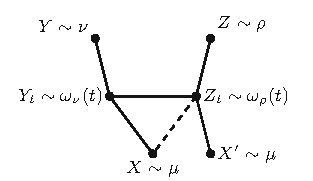
\includegraphics[width=0.65\linewidth]{assets/chapter7/fig7-1.pdf}
\caption{$(\mu,\nu,\rho,\omega_\nu(t),\omega_\rho(t))$ 之间的耦合 $\Upsilon_t$. 实线表示最优耦合；虚线与缺失的连线表示可能次优的耦合.}\label{fig:7.1}
\end{figure}
其中使用了 $\mathbf H=\mathbb R^d$ 时的\autoref{lem:7.10}. 现在注意，$X$ 与 $Z_t$ 的耦合可能次优，因此
$$(1-t)\mathbb E\lVert X-Z_t\rVert^2\ge(1-t)W_2^2(\mu,\omega_\rho(t))
=t^2(1-t)W_2^2(\mu,\rho).$$
此外，再次使用\autoref{lem:7.10}，得到
$$\begin{aligned}
t\mathbb E\lVert Y-Z_t\rVert^2
&=t\mathbb E\lVert Y-(1-t)X'+tZ\rVert^2\\
&=t(1-t)\mathbb E\lVert Y-X'\rVert^2+t^2\mathbb E\lVert Y-Z\rVert^2-t^2(1-t)\mathbb E\lVert X'-Z\rVert^2\\
&\ge t(1-t)\mathbb E\lVert Y-X\rVert^2+t^2\mathbb E\lVert Y-Z\rVert^2-t^2(1-t)\mathbb E\lVert X'-Z\rVert^2,
\end{aligned}$$
其中不等式使用 $X$ 与 $Y$ 最优耦合. 将以上两式代入 \eqref{eq:7.16}，可见含 $\mathbb E\lVert Y-X\rVert^2$ 的项抵消，得到
$$\begin{aligned}
W_2^2(\omega_\nu(t),\omega_\rho(t))
&\ge t^2(1-t)W_2^2(\mu,\rho)+t^2\mathbb E\lVert Y-Z\rVert^2-t^2(1-t)\mathbb E\lVert X'-Z\rVert^2\\
&=t^2\mathbb E\lVert Y-Z\rVert^2.
\end{aligned}$$
回顾 \eqref{eq:7.15}，有 $W_2(\omega_\nu(t),\omega_\rho(t))=O(t)$，故 $\mathbb E\lVert Y_t-Z_t\rVert^2=O(t^2)$. 由于
$$X=(Y_t-tY)/(1-t)\qquad\text{且}\qquad X'=(Z_t-tZ)/(1-t),$$
还可推出 $\mathbb E\lVert X-X'\rVert^2=O(t^2)$. 不加论证地假设 $T_{\mu\to\rho}$ 为 Lipschitz，\footnote{可通过逼近论证去掉这个假设，但需要额外的技术处理.} 则
$$\begin{aligned}
\mathbb E\lVert Y-Z\rVert^2
&=\mathbb E\lVert T_{\mu\to\nu}(X)-T_{\mu\to\rho}(X')\rVert^2\\
&=\mathbb E\lVert T_{\mu\to\nu}(X)-T_{\mu\to\rho}(X)\rVert^2-O(t).
\end{aligned}$$
由此立即得到
$$\lim_{t\searrow0}\frac{W_2^2(\omega_\nu(t),\omega_\rho(t))}{t^2}
\ge\lVert T_{\mu\to\nu}-T_{\mu\to\rho}\rVert_{L^2(\mu)}^2,$$
从而完成引理的证明.
\end{proof}

由\autoref{lem:7.22}，
\begin{equation}\label{eq:7.17}
\begin{aligned}
\cos\measuredangle(\omega_\nu,\omega_\rho)
&=\frac{W_2^2(\mu,\nu)+W_2^2(\mu,\rho)-\lVert T_{\mu\to\nu}-T_{\mu\to\rho}\rVert_{L^2(\mu)}^2}{2W_2(\mu,\nu)W_2(\mu,\rho)}\\
&=\frac{\lVert T_{\mu\to\nu}-\mathrm{id}\rVert_{L^2(\mu)}^2+\lVert T_{\mu\to\rho}-\mathrm{id}\rVert_{L^2(\mu)}^2-\lVert T_{\mu\to\nu}-T_{\mu\to\rho}\rVert_{L^2(\mu)}^2}{2\lVert T_{\mu\to\nu}-\mathrm{id}\rVert_{L^2(\mu)}\lVert T_{\mu\to\rho}-\mathrm{id}\rVert_{L^2(\mu)}}\\
&=\cos\measuredangle(T_{\mu\to\nu}-\mathrm{id},T_{\mu\to\rho}-\mathrm{id}),
\end{aligned}
\end{equation}
其中最后的余弦是在 Hilbert 空间 $L^2(\mu)$ 中理解的. 进而，余弦定理 \eqref{eq:7.13} 表明，$\mu$ 处切锥的度量为
$$\begin{aligned}
\mathsf d_\mu^2((\omega_\nu,s),(\omega_\rho,t))
&=s^2+t^2-2st\cos\measuredangle(\omega_\nu,\omega_\rho)\\
&=s^2+t^2-2st\cos\measuredangle(T_{\mu\to\nu}-\mathrm{id},T_{\mu\to\rho}-\mathrm{id})\\
&=\lVert s(T_{\mu\to\nu}-\mathrm{id})-t(T_{\mu\to\rho}-\mathrm{id})\rVert_{L^2(\mu)}^2.
\end{aligned}$$
因此，配备度量 $\mathsf d_\mu$ 的切锥与某个 Hilbert 空间等距. 我们已证明如下定理；\autoref{sec:5.4}用 Otto 微积分形式体系时，已经识别出这一结果.
\begin{theorem}\label{thm:7.23}
设 $\mu\in\mathcal P_{2,\mathrm{ac}}(\mathbb R^d)$. 则 $\mu$ 处的切锥 $T_\mu\mathcal W_2(\mathbb R^d)$ 是 $L^2(\mu)$ 的一个凸子集. 此外，对任意 $\nu\in\mathcal P_2(\mathbb R^d)$，有
$$\log_\mu(\nu)=T_{\mu\to\nu}-\mathrm{id}\in L^2(\mu),$$
其中 $T_{\mu\to\nu}$ 是从 $\mu$ 到 $\nu$ 的 Brenier 映射.
\end{theorem}
在上述情形中，配备\autoref{def:7.18}中 $\langle\cdot,\cdot\rangle$ 的切锥 $T_\mu\mathcal W_2$ 实际上是 Hilbert 空间的一个凸子集，我们略微滥用术语，称其为 $\mu$ 处的切空间（tangent space）. 从对数映射定义立即可知，对任意 $\nu,\rho\in\mathcal P_2(\mathbb R^d)$，内积 $\langle\cdot,\cdot\rangle_\mu$ 为
$$\begin{aligned}
\langle\log_\mu(\nu),\log_\mu(\rho)\rangle_\mu
&=\langle T_{\mu\to\nu}-\mathrm{id},T_{\mu\to\rho}-\mathrm{id}\rangle_{L^2(\mu)}\\
&=\int\langle T_{\mu\to\nu}(x)-x,T_{\mu\to\rho}(x)-x\rangle\,\mu(dx).
\end{aligned}$$

\subsection{讨论}\label{sec:7.4}
\paragraph{\autoref{sec:7.1}}
Wasserstein 测地线的详细讨论见\cite[第5章]{ref315}与\cite[第7章]{ref18}. 更一般地，任意长度空间上的 Wasserstein 空间也是长度空间.

\paragraph{\autoref{sec:7.2}}
Wasserstein 空间的非负曲率在\cite[第7.3节]{ref18}中证明. 更一般地，非负曲率 Alexandrov 空间上的 Wasserstein 空间也是非负弯曲的.

\autoref{exer:7.2}中的曲线称为广义\index{geodesic@测地线（geodesic）!generalized@广义形式（generalized）|hyperpage}测地线（generalized geodesic），它在 Wasserstein 梯度流理论中起重要作用，有时也用于最优传输的其他应用.

如\autoref{sec:6.1}的讨论说明所提及，有一种适用于测地空间的综合 Ricci 曲率下界概念. 自然会问：为 Wasserstein 空间配备适当测度后，这个概念能否恢复它的非负 Alexandrov 曲率？遗憾的是，文献\cite{ref87}说明，即使是实数轴上平坦的 Wasserstein 空间，也不能由此得到有限的曲率下界.

\paragraph{\autoref{sec:7.3}}
Wasserstein 空间的切锥及其与切空间的关系，见\cite[第12.4节]{ref18}.

\subsection{习题}\label{sec:7.5}
\begin{exercise}\label{exer:7.1}
证明，配备 MMD（\autoref{def:2.20}）的概率测度空间定义了平坦的几何.
\end{exercise}

\begin{exercise}\label{exer:7.2}
设 $\mu,\nu,\rho\in\mathcal P_2(\mathbb R^d)$. 证明存在曲线 $\omega:[0,1]\to\mathcal P_2(\mathbb R^d)$，满足 $\omega(0)=\mu$、$\omega(1)=\nu$，且\autoref{thm:7.15}中的反向不等式成立，即
$$W_2^2(\rho,\omega(t))\le(1-t)W_2^2(\rho,\mu)+tW_2^2(\rho,\nu)-t(1-t)W_2^2(\mu,\nu).$$
提示：对 $X_\mu\sim\mu$、$X_\nu\sim\nu$、$X_\rho\sim\rho$，将 $(X_\mu,X_\rho)$ 与 $(X_\nu,X_\rho)$ 最优耦合. 将 $\omega(t)$ 定义为 $X_\mu$ 与 $X_\nu$ 的适当插值的分布. 与\autoref{sec:5}的\autoref{exer:5.9}比较.
\end{exercise}

\begin{exercise}\label{exer:7.3}
推广\autoref{thm:7.6}的证明，说明对任意 $p\ge1$，有限 $p$ 阶矩概率测度构成的空间 $\mathcal P_p(\mathbb R^d)$，配备 $p$-Wasserstein 度量 $W_p$ 后，是测地空间. 测地线是什么？
\end{exercise}

\begin{exercise}\label{exer:7.4}
推广\autoref{def:7.19}，依照如下提纲证明：若 $(S,\mathsf d)$ 是直径至多为 $\pi$ 的度量空间，$\operatorname{cone}(S)$ 是将 $X\times[0,\infty)$ 中所有形如 $(x,0)$ 的点等同后得到的集合，则
$$\mathsf d((x,s),(y,t)):=\sqrt{s^2+t^2-2st\cos\mathsf d(x,y)}$$
在 $\operatorname{cone}(S)$ 上定义一个度量. 为此，取锥中的三个点 $(x_1,r_1)$、$(x_2,r_2)$、$(x_3,r_3)$，在 $\mathbb R^2$ 中构造三个点 $y_1,y_2,y_3$，使它们到原点的距离分别为 $r_1,r_2,r_3$，且 $y_1,y_2$ 之间的角和 $y_2,y_3$ 之间的角分别等于 $\mathsf d(x_1,x_2)$ 与 $\mathsf d(x_2,x_3)$. 证明 $\lVert y_1-y_2\rVert=\mathsf d((x_1,r_1),(x_2,r_2))$ 与 $\lVert y_2-y_3\rVert=\mathsf d((x_2,r_2),(x_3,r_3))$. 注意：$\lVert y_1-y_3\rVert$ 未必等于 $\mathsf d((x_1,r_1),(x_3,r_3))$. 现在按 $\mathsf d(x_1,x_2)+\mathsf d(x_2,x_3)\le\pi$ 是否成立分两种情形，建立锥度量的三角不等式.
\end{exercise}

\section{Wasserstein重心}\label{sec:8}
数据平均是统计学家最基本的工具之一；但如果在非欧几里得空间中实现平均，用以刻画不同于传统统计文献中常见的向量值协变量的数据类型，通常就必须格外谨慎. 例如，假设数据集由图像组成，我们希望定义适当的“平均图像”，以捕捉整个数据集具有代表性的方面. 这一典型问题会出现在汇总重复 MRI 扫描信息等场景中.

可以通过每个像素在 R、G、B 通道中的值来表示一幅有 $p$ 个像素的图像，从而将其视为取值于 $\{0,1,\ldots,255\}^{3p}$ 的向量. 一种朴素的平均方法，是直接计算图像这些向量表示的通常平均值. 不过，读者只要对几幅图像尝试一下，就应当很容易确信，这样的平均概念并不令人满意.

仔细考察这一朴素方法，可以看出问题的实质：当我们对图像的向量表示作平均时，实际上默默地赋予空间 $\mathbb R^{3p}$ 以欧几里得几何；但没有理由期待这一几何与图像到 $\mathbb R^{3p}$ 的嵌入相容. 事实上，将图像表示为 $\mathbb R^{3p}$ 中的向量是一种工程选择，而非图像的内在属性. 或许更有原则的方法，是将图像视为某个抽象空间 $S$ 中的元素，为其赋予度量 $\mathsf d$，以刻画所研究数据在重要属性上的接近程度. 于是，任务可表述为：给定度量空间 $(S,\mathsf d)$ 中的点 $x_1,\ldots,x_n$，它们的平均应当如何适当定义？

幸运的是，这一问题有一个一般而有用的答案，其动机如下. 不难看出，对于 Hilbert 空间 $\mathbf H$ 中的 $x_1,\ldots,x_n$，平均 $\frac1n\sum_{i=1}^n x_i$ 可以刻画为泛函
$$x\longmapsto\frac1n\sum_{i=1}^n\|x_i-x\|^2$$
的唯一极小化解. 这一表述只涉及平方距离，因此可以推广到度量空间.
\begin{definition}[重心]\label{def:8.1}\index{barycenter@重心（barycenter）|hyperpage}
给定度量空间 $(S,\mathsf d)$ 上任意概率测度 $P$，如果 $b$ 是泛函
$$b\longmapsto\int\mathsf d^2(b,x)\,P(dx)$$
的极小化解，则称 $b$ 是 $P$ 的一个重心（barycenter）.
\end{definition}
特别地，如果取 $P$ 为经验测度 $\frac1n\sum_{i=1}^n\delta_{x_i}$，那么 $P$ 的重心就是点 $x_1,\ldots,x_n$ 的一种平均. 注意，在如此一般的层次上，重心可能不存在；即使存在，也可能不唯一.

$(S,\mathsf d)$ 为 Wasserstein 空间的情形本身就很有意义，也是本章理论发展的动机. 例如，Wasserstein 重心为本章开头的图像平均问题，以及曲线配准（curve registration）等许多其他问题，提供了具有几何意义的解；见\cite{ref48,ref98,ref155,ref198,ref252,ref257,ref266,ref289,ref290}及其中的参考文献. 不过，由于我们发展的框架自然适合\autoref{sec:7}所介绍的度量几何，因此先在这一背景下工作，再讨论特殊情形.

这里发展统计理论，以说明实际应用几何平均方法的合理性. 具体地，假设有来自 $(S,\mathsf d)$ 上分布 $P$ 的独立同分布数据 $X_1,\ldots,X_n$，以 $b^\star$ 表示 $P$ 的重心. 这个总体重心是所关心的未知量. 为使统计问题良定，我们始终采用能够保证 $b^\star$ 存在且唯一的假设.

这一问题有一个自然的代入估计量：经验测度的重心 $b_n$，也称经验重心（empirical barycenter），定义为泛函
$$b\longmapsto\frac1n\sum_{i=1}^n\mathsf d^2(b,X_i)$$
的极小化解. 目标是根据空间 $(S,\mathsf d)$ 自然的几何特征，量化误差 $\mathsf d(b_n,b^\star)$.

\subsection{Hilbert 空间情形}\label{sec:8.1}
当 $(S,\mathsf d)$ 为 Hilbert 空间时，经验重心以所谓参数速率收敛. 这一点很容易看出. 为此，令 $\mathbf H$ 为 Hilbert 空间，并回顾此时
$$b_n=\frac1n\sum_{i=1}^n X_i,\qquad b^\star=\mathbb EX=\int x\,P(dx),$$
其中使用 Pettis 积分定义 $b^\star$. 有
$$\begin{aligned}
\mathbb E\|b_n-b^\star\|^2&=\frac1{n^2}\sum_{i,j=1}^n
\mathbb E\langle X_i-\mathbb EX,X_j-\mathbb EX\rangle\\
&=\frac1n\operatorname{var}(X),\qquad
\operatorname{var}(X)=\mathbb E\|X-\mathbb EX\|^2,
\end{aligned}$$
其中使用了 $X_i$ 的独立性与内积的双线性. 遗憾的是，这一证明虽然简洁，还得到了等式（！），但启发性并不很强，因为它关键地使用了重心的闭式表达和内积结构，而这些都无法推广到 Hilbert 空间之外.

值得注意的是，在非正曲率空间（NPC space）中，重心估计仍具有相同的参数速率，见\autoref{exer:8.2}. 不过，如\autoref{thm:7.15}所示，最主要的研究对象 Wasserstein 空间是一个非负曲率空间（NNC space）. 因此，目标是在更困难的 $\operatorname{curv}\ge0$ 情形下发展统计理论.

回到 Hilbert 情形以获取启发. 我们提出第二种证明，它仍给出定性相同的结果，但差一个因子 4. 根据 $b_n$ 的定义，
$$P_n\|b_n-\bullet\|^2\le P_n\|b^\star-\bullet\|^2.$$
这里及后文采用简写的算子记号：对任意可积函数 $f$，$Pf(\bullet)=\int f(x)P(dx)$；特别地，
$$P_nf(\bullet)=\frac1n\sum_{i=1}^n f(X_i),\qquad
P_n=\frac1n\sum_{i=1}^n\delta_{X_i}$$
表示 $X_i$ 的经验分布. 再注意到
$$\|b_n-\bullet\|^2=\|b_n-b^\star\|^2+\|b^\star-\bullet\|^2
+2\langle b_n-b^\star,b^\star-\bullet\rangle.$$
因此，应用算子 $P_n$，得到
$$\|b_n-b^\star\|^2+P_n\|b^\star-\bullet\|^2
+2P_n\langle b_n-b^\star,b^\star-\bullet\rangle\le P_n\|b^\star-\bullet\|^2,$$
所以
$$\|b_n-b^\star\|^2\le2P_n\langle b_n-b^\star,\bullet-b^\star\rangle.$$
上述不等式其实只是在说 $\|b_n-b^\star\|^2\le2\|b_n-b^\star\|^2$，并没有太大用处；但为了展示论证思路，仍继续沿这条路走下去.

首先，由内积的线性，
$$P\langle b_n-b^\star,\bullet-b^\star\rangle=0.$$
因此
$$\begin{aligned}
\|b_n-b^\star\|^2&\le2(P_n-P)\langle b_n-b^\star,\bullet-b^\star\rangle\\
&=2\langle b_n-b^\star,(P_n-P)(\bullet-b^\star)\rangle.
\end{aligned}$$
两边除以 $\|b_n-b^\star\|$，并应用 Cauchy--Schwarz 不等式，得到
\begin{equation}\label{eq:8.1}
\mathbb E\|b_n-b^\star\|^2\le4\mathbb E\|(P_n-P)(\bullet-b^\star)\|^2
=\frac4n\operatorname{var}(X).
\end{equation}
这一证明带来了什么？首先，只得到了不等式，并损失一个因子 4. 主要收获是，从未使用 $b_n$ 的闭式表达. 只使用了
$$\mathbb E\|(P_n-P)(\bullet-b^\star)\|^2\le\operatorname{var}(X)/n,$$
而这一事实适用得更广. 不利的一面是，仍大量使用了内积的线性，以及更一般的 Hilbert 结构. 事实证明，要得到我们的结果，这些结构相当必要. 因此，我们将通过 $\mathcal W_2$ 的切空间引入 Hilbert 结构，并追踪由此产生的损失.

\subsection{正曲率空间上的重心}\label{sec:8.2}
设 $P$ 是正曲率测地空间 $(S,\mathsf d)$ 上的概率测度. 令 $b^\star$ 为 $P$ 的任意一个重心，以 $b_n$ 表示由 $X\sim P$ 的 $n$ 个独立副本 $X_1,\ldots,X_n$ 构造的经验重心：
$$\begin{aligned}
b^\star&\in\operatorname*{arg\,min}_{b\in S}\int\mathsf d^2(b,x)\,P(dx),\\
b_n&\in\operatorname*{arg\,min}_{b\in S}\sum_{i=1}^n\mathsf d^2(b,X_i).
\end{aligned}$$
在继续之前，先讨论整体思路. Hilbert 情形的论证依赖于不等式 $P_n\mathsf d^2(b_n,\bullet)\le P_n\mathsf d^2(b^\star,\bullet)$；它由 $b_n$ 的定义成立，也表明经验重心是统计估计文献中经验风险\index{empirical risk minimization (ERM)@经验风险最小化（ERM）（empirical risk minimization (ERM)）|hyperpage}最小化框架的一个实例. 利用经验风险最小化技术，可能希望通过空间 $(S,\mathsf d)$ 的“复杂度”度量来控制估计误差；文献中已有沿这一路径的工作（见\cite{ref4}）. 不过，对于所关心的 Wasserstein 空间应用，其复杂度过大，会导致非参数估计速率；特别地，与\autoref{sec:2}中的情形类似，这些速率受到维数灾难的影响.

然而，刚刚已经看到，Hilbert 空间中的估计速率可以避开维数灾难，即使 Hilbert 空间可以是无限维的. 因此，直觉使我们相信：即使在弯曲空间 $(S,\mathsf d)$ 上工作，只要能将研究限制在 $S$ 足够“平坦”的部分，或许也可以恢复 Hilbert 型速率. 后文将寻找自然的几何条件；本质上，它们编码了曲率界，使快速的参数估计速率成为可能.

\subsubsection{主定理}\label{sec:8.2.1}
先给出一个一般结果，模仿\autoref{sec:8.1}中 Hilbert 情形的证明.

在陈述之前，引入一个量，用来衡量重心 $b^\star$ 处的切空间在该点附近与原空间“贴合”的程度.
\begin{definition}[贴合]\label{def:8.2}\index{hugging@贴合函数（hugging）|hyperpage}
设 $(S,\mathsf d)$ 为满足 $\operatorname{curv}(S)\ge0$ 的测地空间. 对任意 $b^\star,b\in S$，令 $h_{b^\star}^b$ 为 $S$ 在 $b^\star$ 处沿 $b$ 方向的贴合函数（hugging function），定义为
\begin{equation}\label{eq:8.2}
h_{b^\star}^b(x)=1-
\frac{\|\log_{b^\star}(x)-\log_{b^\star}(b)\|_{b^\star}^2-\mathsf d^2(x,b)}
{\mathsf d^2(b,b^\star)},\qquad x\in S.
\end{equation}
\end{definition}
注意，由\autoref{prop:7.21}，对所有 $x\in S$ 都有 $h_{b^\star}^b(x)\le1$. 此外，如果 $S$ 为 Hilbert 空间，则 $\|\log_{b^\star}(x)-\log_{b^\star}(b)\|_{b^\star}^2=\mathsf d^2(x,b)$，且 $h_{b^\star}^b\equiv1$. 一般地，当 $b^\star$ 周围存在大量曲率时，$h_{b^\star}^b(x)$ 可能为负；但在重心 $b^\star$ 处计算时，它的平均仍保持非负. 这一结果来自下面这个简单而重要的观察.
\begin{theorem}[方差等式]\label{thm:8.3}\index{variance equality@方差等式（variance equality）|hyperpage}
设 $(S,\mathsf d)$ 为满足 $\operatorname{curv}(S)\ge0$ 的测地空间. 令 $Q\in\mathcal P_2(S)$ 是 $S$ 上的概率分布，重心为 $b^\star$. 进一步假设，$S$ 在 $b^\star$ 处的切锥赋予 $\langle\cdot,\cdot\rangle_{b^\star}$ 后，是某个 Hilbert 空间的凸子集. 那么，对所有 $b\in S$，
\begin{equation}\label{eq:8.3}
\mathsf d^2(b,b^\star)\int h_{b^\star}^b(x)\,Q(dx)
=\int\bigl(\mathsf d^2(x,b)-\mathsf d^2(x,b^\star)\bigr)\,Q(dx),
\end{equation}
其中 $h_{b^\star}^b$ 是 \eqref{eq:8.2} 定义的贴合函数.
\end{theorem}
\begin{proof}
由 $h_{b^\star}^b$ 的定义，有
$$\begin{aligned}
\mathsf d^2(b,b^\star)h_{b^\star}^b(\bullet)
={}&\mathsf d^2(b,b^\star)+\mathsf d^2(\bullet,b)
-\|\log_{b^\star}b-\log_{b^\star}\bullet\|_{b^\star}^2\\
={}&\mathsf d^2(b,b^\star)+\mathsf d^2(\bullet,b)
-\|\log_{b^\star}b\|_{b^\star}^2-\|\log_{b^\star}\bullet\|_{b^\star}^2\\
&+2\langle\log_{b^\star}\bullet,\log_{b^\star}b\rangle_{b^\star}\\
={}&\mathsf d^2(b,b^\star)+\mathsf d^2(\bullet,b)
-\mathsf d^2(b,b^\star)-\mathsf d^2(b^\star,\bullet)\\
&+2\langle\log_{b^\star}\bullet,\log_{b^\star}b\rangle_{b^\star}\\
={}&\mathsf d^2(\bullet,b)-\mathsf d^2(\bullet,b^\star)
+2\langle\log_{b^\star}\bullet,\log_{b^\star}b\rangle_{b^\star}.
\end{aligned}$$
因此，应用线性算子 $Q$，得到
$$\begin{aligned}
\mathsf d^2(b,b^\star)Qh_{b^\star}^b(\bullet)
={}&Q\mathsf d^2(\bullet,b)-Q\mathsf d^2(\bullet,b^\star)\\
&+2\langle\log_{b^\star}b^\star,\log_{b^\star}b\rangle_{b^\star},
\end{aligned}$$
其中使用了 $Q\log_{b^\star}\bullet=\log_{b^\star}b^\star$，换言之，$\log_{b^\star}b^\star$ 是 $(\log_{b^\star})_\#Q$ 的重心. 事实上，由\autoref{prop:7.21}，对所有 $b\in S$，
$$\begin{aligned}
Q\|\log_{b^\star}\bullet-\log_{b^\star}b^\star\|_{b^\star}^2
&=Q\mathsf d^2(\bullet,b^\star)\le Q\mathsf d^2(\bullet,b)\\
&\le Q\|\log_{b^\star}\bullet-\log_{b^\star}b\|_{b^\star}^2,
\end{aligned}$$
且当 $b=b^\star$ 时等号成立，所以 $\log_{b^\star}b^\star$ 是 $(\log_{b^\star})_\#Q$ 的一个重心，从而 $Q\log_{b^\star}\bullet=\log_{b^\star}b^\star$.

最后，由于 $\log_{b^\star}b^\star=o_{b^\star}$ 为切锥的顶点，有 $\|\log_{b^\star}b^\star\|_{b^\star}=0$，进而 $\langle\log_{b^\star}b^\star,\log_{b^\star}b\rangle_{b^\star}=0$. 证明完毕.
\end{proof}

方差等式的一个直接推论是，如果 $\int h_{b^\star}^b\,dQ>0$，则 $b^\star$ 是 $Q$ 的唯一重心. 此外，由重心 $b^\star$ 的定义，方差等式右端非负，因此立即得到下面的推论.
\begin{corollary}\label{cor:8.4}
在与\autoref{thm:8.3}相同的假设下，对任意 $b\in S$，
$$0\le\int h_{b^\star}^b(x)\,Q(dx)\le1.$$
此外，对任意 $b,x\in S$，有 $h_{b^\star}^b(x)\le1$.
\end{corollary}

事实证明，$b^\star$ 处的贴合函数，是得到经验重心参数收敛速率的关键.
\begin{theorem}[主定理]\label{thm:8.5}
设 $P$ 是非负曲率测地空间 $(S,\mathsf d)$ 上的概率测度，$b^\star,b_n$ 分别表示 $P$ 的一个重心和一个经验重心. 进一步假设，$S$ 在 $b^\star$ 处的切锥赋予 $\langle\cdot,\cdot\rangle_{b^\star}$ 后，是某个 Hilbert 空间的凸子集. 那么，如果对任意 $b\in S$，都有
\begin{equation}\label{eq:8.4}
h_{b^\star}^b(\bullet)\ge h_{\min}>0,
\end{equation}
则 $b_n,b^\star$ 都唯一，且
$$\mathbb E\mathsf d^2(b_n,b^\star)\le\frac{4\sigma^2}{h_{\min}^2n},$$
其中 $\sigma^2$ 表示 $P$ 的方差，定义为
\begin{equation}\label{eq:8.5}
\sigma^2=\int\mathsf d^2(b^\star,x)\,P(dx).
\end{equation}
\end{theorem}
\begin{proof}
首先，唯一性直接由方差等式与 \eqref{eq:8.4} 得到.

接着，与 Hilbert 情形一样，先观察到
$$P_n\mathsf d^2(b_n,\bullet)\le P_n\mathsf d^2(b^\star,\bullet).$$
这给出
\begin{equation}\label{eq:8.6}
\begin{aligned}
&P_n\mathsf d^2(b_n,\bullet)-P_n\|\log_{b^\star}b_n-\log_{b^\star}\bullet\|_{b^\star}^2\\
&\quad+P_n\|\log_{b^\star}b_n-\log_{b^\star}\bullet\|_{b^\star}^2
-P_n\mathsf d^2(b^\star,\bullet)\le0.
\end{aligned}
\end{equation}
现在利用切锥具有 Hilbert 结构这一事实，得到
$$\begin{aligned}
\|\log_{b^\star}b_n-\log_{b^\star}\bullet\|_{b^\star}^2
&=\|\log_{b^\star}b_n\|_{b^\star}^2+\|\log_{b^\star}\bullet\|_{b^\star}^2
-2\langle\log_{b^\star}b_n,\log_{b^\star}\bullet\rangle_{b^\star}\\
&=\mathsf d^2(b^\star,b_n)+\mathsf d^2(b^\star,\bullet)
-2\langle\log_{b^\star}b_n,\log_{b^\star}\bullet\rangle_{b^\star},
\end{aligned}$$
第二个恒等式两次使用了\autoref{prop:7.21}的取等情形. 代入 \eqref{eq:8.6}，得到
$$\begin{aligned}
\mathsf d^2(b^\star,b_n)\le{}&P_n[\|\log_{b^\star}b_n-\log_{b^\star}\bullet\|_{b^\star}^2
-\mathsf d^2(b_n,\bullet)]\\
&+2P_n\langle\log_{b^\star}b_n,\log_{b^\star}\bullet\rangle_{b^\star}.
\end{aligned}$$
接着，由贴合函数的定义，
$$\|\log_{b^\star}b_n-\log_{b^\star}\bullet\|_{b^\star}^2-\mathsf d^2(b_n,\bullet)
=(1-h_{b^\star}^{b_n}(\bullet))\mathsf d^2(b_n,b^\star).$$
从而
$$h_{\min}\mathsf d^2(b_n,b^\star)
\le2P_n\langle\log_{b^\star}b_n,\log_{b^\star}\bullet\rangle_{b^\star}.$$
右端只是 Hilbert 空间中的平均，因此两边除以 $\|\log_{b^\star}b_n\|_{b^\star}=\mathsf d(b_n,b^\star)$，并应用 Cauchy--Schwarz 不等式，得到
$$h_{\min}^2\mathbb E\mathsf d^2(b_n,b^\star)\le\frac{4\sigma^2}n,$$
其中
$$\sigma^2=\int\|\log_{b^\star}x\|_{b^\star}^2\,P(dx)
=\int\mathsf d^2(b^\star,x)\,P(dx),$$
即为所求.
\end{proof}

检查主定理的证明可知，为得到 $b^\star$ 的参数估计速率，更弱的条件 $P_nh_{b^\star}^{b_n}(\bullet)\ge h_{\min}>0$ 已经足够. 由于 $P_n$ 是随机测度，我们倾向于不对它施加条件，而着重研究更强的条件 \eqref{eq:8.4}. 接下来将利用可延拓测地线这一概念得到这类结果.

\subsubsection{可延拓测地线}\label{sec:8.2.2}
现在给出一个有说服力的综合几何条件，它在非负曲率空间中蕴含上述下界：所有从重心 $b^\star$ 出发以及到达该点的测地线，都能按给定因子延拓.
\begin{definition}[可延拓测地线]\label{def:8.6}\index{geodesic@测地线（geodesic）!extendable@可延拓（extendable）|hyperpage}
考虑常速测地线 $\omega:[0,1]\to S$. 对 $(\lambda_{\mathrm{in}},\lambda_{\mathrm{out}})\in[0,\infty]^2$，如果存在路径 $\omega^+:[-\lambda_{\mathrm{in}},1+\lambda_{\mathrm{out}}]\to S$，在 $[0,1]$ 上与 $\omega$ 一致，并且在端点 $\omega^+(-\lambda_{\mathrm{in}})$ 与 $\omega^+(1+\lambda_{\mathrm{out}})$ 之间仍为测地线，则称 $\omega$ 是 $(\lambda_{\mathrm{in}},\lambda_{\mathrm{out}})$-可延拓的（extendable）. 路径 $\omega^+$ 称为 $\omega$ 的一个延拓.
\end{definition}
陈述本小节的主要结果之前，需要下面的事实.
\begin{theorem}\label{thm:8.7}
假设 $\operatorname{curv}(S)\ge0$. 设 $Q\in\mathcal P_2(S)$ 是 $S$ 上的概率测度，重心为 $b^\star$. 假设对每个 $x\in\operatorname{supp}(Q)$，都存在一条连接 $b^\star$ 与 $x$ 的常速测地线 $\omega_x:[0,1]\to S$，它对 $\lambda>0$ 是 $(0,\lambda)$-可延拓的. 再假设 $b^\star$ 仍然是分布 $Q_\lambda=(e_\lambda)_\#Q$ 的重心，其中 $e_\lambda(x)=\omega_x^+(1+\lambda)$. 那么，对所有 $b\in S$，
\begin{equation}\label{eq:8.7}
Qh_{b^\star}^b(\bullet)\ge\frac\lambda{1+\lambda}.
\end{equation}
特别地，这意味着 $b^\star$ 是 $Q$ 的唯一重心.
\end{theorem}
\begin{proof}
固定 $y\in\operatorname{supp}(Q)$，定义 $y_\lambda=e_\lambda(y)$. 令 $\omega:[0,1]\to S$ 为连接 $b^\star$ 与 $y_\lambda$ 的常速测地线. 根据定义，对 $\tau=1/(1+\lambda)$ 有 $\omega(\tau)=y$. 由于 $\operatorname{curv}(S)\ge0$，对任意 $b\in S$，
$$\begin{aligned}
\mathsf d^2(b,y)&\ge(1-\tau)\mathsf d^2(b,b^\star)+\tau\mathsf d^2(b,y_\lambda)
-\tau(1-\tau)\mathsf d^2(b^\star,y_\lambda)\\
&=\frac\lambda{1+\lambda}\mathsf d^2(b,b^\star)
+\frac1{1+\lambda}\mathsf d^2(b,y_\lambda)
-\frac\lambda{(1+\lambda)^2}\mathsf d^2(b^\star,y_\lambda).
\end{aligned}$$
再注意到
$$\mathsf d^2(b^\star,y_\lambda)=(1+\lambda)^2\mathsf d^2(b^\star,y),$$
因此
\begin{equation}\label{eq:8.8}
\begin{aligned}
\frac\lambda{1+\lambda}\mathsf d^2(b,b^\star)
&\le\mathsf d^2(b,y)+\lambda\mathsf d^2(b^\star,y)-\frac1{1+\lambda}\mathsf d^2(b,y_\lambda)\\
&=(\mathsf d^2(b,y)-\mathsf d^2(b^\star,y))
+(1+\lambda)\mathsf d^2(b^\star,y)-\frac1{1+\lambda}\mathsf d^2(b,y_\lambda).
\end{aligned}
\end{equation}
此外，
$$\begin{aligned}
&(1+\lambda)\mathsf d^2(b^\star,y)-\frac1{1+\lambda}\mathsf d^2(b,y_\lambda)\\
&\quad=\frac1{1+\lambda}\bigl((1+\lambda)^2\mathsf d^2(b^\star,y)-\mathsf d^2(b,y_\lambda)\bigr)\\
&\quad=\frac1{1+\lambda}\bigl(\mathsf d^2(b^\star,y_\lambda)-\mathsf d^2(b,y_\lambda)\bigr).
\end{aligned}$$
因此，记 $Q_\lambda:=(e_\lambda)_\#Q$，得到
$$\begin{aligned}
&\int\left((1+\lambda)\mathsf d^2(b^\star,y)-\frac1{1+\lambda}\mathsf d^2(b,y_\lambda)\right)Q(dy)\\
&\quad=\frac1{1+\lambda}\int\bigl(\mathsf d^2(b^\star,y)-\mathsf d^2(b,y)\bigr)Q_\lambda(dy)\le0,
\end{aligned}$$
最后一步利用了 $b^\star$ 仍为 $Q_\lambda$ 的重心这一事实. 与对 \eqref{eq:8.8} 关于 $Q$ 积分所得结果结合，得到
\begin{equation}\label{eq:8.9}
\frac\lambda{1+\lambda}\mathsf d^2(b,b^\star)
\le\int\bigl(\mathsf d^2(b,y)-\mathsf d^2(b^\star,y)\bigr)Q(dy).
\end{equation}
结合方差等式（\autoref{thm:8.3}），证明完成.
\end{proof}

上述可延拓测地线概念给出 $Ph_{b^\star}^b(\bullet)$ 关于 $b$ 的一致下界. 这一性质已经相当有吸引力，因为它蕴含重心的唯一性，但仍有两个不足. 第一，需要控制 $P_nh_{b^\star}^{b_n}(\bullet)$，而 $b_n$ 依赖于数据；尚不清楚如何适当地控制偏差 $|P_nh_{b^\star}^{b_n}-Ph_{b^\star}^{b_n}|$. 第二，$P_\lambda=(e_\lambda)_\#P$ 保持相同重心这一条件难以检验，似乎也比较苛刻.

为克服这两个限制，允许从 $b^\star$ 出发的测地线向两个方向延拓.
\begin{theorem}\label{thm:8.8}
假设 $\operatorname{curv}(S)\ge0$，且 $x,b,b^\star\in S$. 假设存在 $\lambda_{\mathrm{in}},\lambda_{\mathrm{out}}>0$，以及一条连接 $b^\star$ 与 $x$ 的 $(\lambda_{\mathrm{in}},\lambda_{\mathrm{out}})$-可延拓测地线. 那么
$$h_{b^\star}^b(x)\ge h_{\min}
=\frac{\lambda_{\mathrm{out}}}{1+\lambda_{\mathrm{out}}}-\frac1{\lambda_{\mathrm{in}}}.$$
\end{theorem}
\begin{proof}
令 $\omega_x:[0,1]\to S$ 为连接 $b^\star$ 与 $x$ 的一条 $(\lambda_{\mathrm{in}},\lambda_{\mathrm{out}})$-可延拓测地线，其延拓记为 $\omega_x^+:[-\lambda_{\mathrm{in}},1+\lambda_{\mathrm{out}}]\to S$. 令 $z=\omega_x^+(-\xi)$，其中 $\xi=\lambda_{\mathrm{in}}/(1+\lambda_{\mathrm{out}})$，并考虑测度
$$Q:=\frac\xi{1+\xi}\delta_x+\frac1{1+\xi}\delta_z.$$
由于 $Q$ 支撑在 $\omega^+$ 上，很容易计算其重心. 事实上，注意 $x=\omega_x^+(1)$，所以 $Q$ 的重心为
$$\omega_x^+\left(1\cdot\frac\xi{1+\xi}-\xi\cdot\frac1{1+\xi}\right)
=\omega^+(0)=b^\star.$$

现在希望将\autoref{thm:8.7}用于 $Q$. 为此，注意连接 $b^\star$ 与 $x$ 的常速测地线 $\omega_x$，以及连接 $b^\star$ 与 $z$、定义为 $\sigma(t)=\omega_x^+(-t\xi)$ 的常速测地线 $\sigma$，分别由假设和构造可知，都是 $(0,1+\lambda_{\mathrm{out}})$-可延拓的.

最后，验证 $b^\star$ 仍为概率测度 $Q_{\lambda_{\mathrm{out}}}=(e_{\lambda_{\mathrm{out}}})_\#Q$ 的重心，其中 $e_{\lambda_{\mathrm{out}}}(x)=\omega_x^+(1+\lambda_{\mathrm{out}})$. 事实上，根据构造，$Q_{\lambda_{\mathrm{out}}}$ 是如下两点概率测度：
$$Q_{\lambda_{\mathrm{out}}}=\frac\xi{1+\xi}\delta_{\omega^+(1+\lambda_{\mathrm{out}})}
+\frac1{1+\xi}\delta_{\omega^+(-\lambda_{\mathrm{in}})}.$$
因此，其重心为
$$\begin{aligned}
&\omega^+\left((1+\lambda_{\mathrm{out}})\cdot\frac\xi{1+\xi}
-\lambda_{\mathrm{in}}\cdot\frac1{1+\xi}\right)\\
&\quad=\omega^+\left(\frac{(1+\lambda_{\mathrm{out}})\lambda_{\mathrm{in}}}{1+\lambda_{\mathrm{in}}+\lambda_{\mathrm{out}}}
-\frac{\lambda_{\mathrm{in}}(1+\lambda_{\mathrm{out}})}{1+\lambda_{\mathrm{in}}+\lambda_{\mathrm{out}}}\right)
=\omega^+(0)=b^\star.
\end{aligned}$$
从而，\autoref{thm:8.7}给出
$$\begin{aligned}
\frac{\lambda_{\mathrm{out}}}{1+\lambda_{\mathrm{out}}}
&\le Qh_{b^\star}^b(\bullet)
=\frac\xi{1+\xi}h_{b^\star}^b(x)+\frac1{1+\xi}h_{b^\star}^b(z)\\
&\le\frac\xi{1+\xi}h_{b^\star}^b(x)+\frac1{1+\xi},
\end{aligned}$$
其中使用\autoref{cor:8.4}，对所有 $b,z\in S$ 有 $h_{b^\star}^b(z)\le1$.

因此得到
$$\begin{aligned}
h_{b^\star}^b(x)&\ge\frac{1+\xi}\xi
\left(\frac{\lambda_{\mathrm{out}}}{1+\lambda_{\mathrm{out}}}-\frac1{1+\xi}\right)\\
&=\frac{1+\xi}\xi\left(\frac{\lambda_{\mathrm{out}}}{\lambda_{\mathrm{in}}}\xi-\frac1{1+\xi}\right)\\
&=\frac{\lambda_{\mathrm{out}}}{\lambda_{\mathrm{in}}}(1+\xi)-\frac1\xi\\
&=\frac{\lambda_{\mathrm{out}}}{\lambda_{\mathrm{in}}}
+\frac{\lambda_{\mathrm{out}}}{\lambda_{\mathrm{in}}}
\frac{\lambda_{\mathrm{in}}}{1+\lambda_{\mathrm{out}}}
-\frac{1+\lambda_{\mathrm{out}}}{\lambda_{\mathrm{in}}}\\
&=\frac{\lambda_{\mathrm{out}}}{1+\lambda_{\mathrm{out}}}-\frac1{\lambda_{\mathrm{in}}},
\end{aligned}$$
证明完毕.
\end{proof}

注意，\autoref{thm:8.8}给出的 $h_{b^\star}^b(x)$ 下界对 $b,x$ 均一致. 当然，也可以使这一结果只依赖于 $x$，得到形如
$$h_{b^\star}^b(x)\ge\frac{\lambda_{\mathrm{out}}(x)}{1+\lambda_{\mathrm{out}}(x)}
-\frac1{\lambda_{\mathrm{in}}(x)}$$
的结果. 如果假设
$$P\left(\frac{\lambda_{\mathrm{out}}(\bullet)}{1+\lambda_{\mathrm{out}}(\bullet)}
-\frac1{\lambda_{\mathrm{in}}(\bullet)}\right)>0,$$
那么标准的集中工具可以保证，当 $n$ 足够大时，有所需的 $P_nh_{b^\star}^{b_n}(\bullet)>0$.

不再深入这些细节，而更仔细地考察一致下界. 主定理与\autoref{thm:8.8}给出下面的推论.
\begin{corollary}\label{cor:8.9}
设 $P$ 是非负曲率测地空间 $(S,\mathsf d)$ 上的概率测度，$b^\star,b_n$ 分别表示 $P$ 的一个重心和一个经验重心. 假设 $b^\star$ 处的切锥赋予 $\langle\cdot,\cdot\rangle_{b^\star}$ 后，是某个 Hilbert 空间的凸子集. 此外，令 $\lambda_{\mathrm{in}},\lambda_{\mathrm{out}}\in[0,\infty]$ 满足
$$h:=\frac{\lambda_{\mathrm{out}}}{1+\lambda_{\mathrm{out}}}-\frac1{\lambda_{\mathrm{in}}}>0,$$
并进一步假设，对任意 $x\in\operatorname{supp}(P)$，都存在一条连接 $b^\star$ 与 $x$ 的 $(\lambda_{\mathrm{in}},\lambda_{\mathrm{out}})$-可延拓测地线. 那么 $b^\star$ 唯一，且经验重心满足
$$\mathbb E[\mathsf d^2(b_n,b^\star)]\le\frac{4\sigma^2}{hn},$$
其中 $\sigma^2$ 为 \eqref{eq:8.5} 定义的 $P$ 的方差.
\end{corollary}
由此，当测地线可以充分延拓时，得到参数速率. 特别地，如果 $S$ 为 Hilbert 空间，则所有测地线都可以无限延拓. 因而 $h=1$，并恢复 \eqref{eq:8.1}.

\subsection{Wasserstein 重心的参数速率}\label{sec:8.3}
作为这些讲义的结尾，以 Wasserstein 重心为例展开研究. 注意，我们的结果可以直接应用于这一情形. 一个自然问题是：可延拓测地线的条件在最优传输中对应什么？事实证明，可以用 Brenier 映射的正则性条件刻画它.
\begin{theorem}\label{thm:8.10}
设 $\mu,\nu\in\mathcal W_2$ 为两个概率测度，$\mu$ 有密度；令 $\varphi:\mathbb R^d\to\mathbb R$ 为凸函数，定义为 $\varphi(x)=(\|x\|^2-f(x))/2$，其中 $f$ 是\autoref{def:1.15}给出的 Kantorovich 势. 特别地，$\nabla\varphi$ 在 $\mu$ 几乎处处有定义，并且是 Brenier 映射. 回顾连接 $\mu$ 与 $\nu$ 的唯一常速测地线 $\omega$ 为 $\omega(t)=((1-t)\mathrm{id}+t\nabla\varphi)_\#\mu$. 那么，对任意 $\lambda>0$，$\omega$ 是 $(0,\lambda)$-可延拓的，当且仅当 $\varphi$ 是 $\lambda/(1+\lambda)$-强凸的.
\end{theorem}
\begin{proof}
先假设 $\omega$ 是 $(0,1+\lambda)$-可延拓的，并以
$$\omega^+:[0,1+\lambda]\to\mathcal W_2$$
表示其延拓. 令 $Y_\lambda\sim\omega^+(1+\lambda)$，注意存在一个在 $\mu$ 几乎处处定义的凸函数 $\varphi_\lambda$，使得 $Y_\lambda=\nabla\varphi_\lambda(X)$，其中 $X\sim\mu$. 此外，由于 $\omega^+$ 是测地线，且 $\nabla\varphi(X)\sim\omega^+(1)$，还有
$$\nabla\varphi(X)=\frac\lambda{1+\lambda}X+\frac1{1+\lambda}Y_\lambda,$$
所以 $Y_\lambda=\nabla\varphi_\lambda(X)=(1+\lambda)\nabla\varphi(X)-\lambda X$. 特别地，这意味着可以选择
$$\varphi(x)=\frac1{1+\lambda}\varphi_\lambda(x)+\frac\lambda{2(1+\lambda)}\|x\|^2.$$
由于 $\varphi_\lambda$ 为凸函数，$\varphi_\lambda/(1+\lambda)$ 也凸，上式因而说明 $\varphi$ 为 $\lambda/(1+\lambda)$-强凸.

反过来，假设 $\varphi$ 是 $\lambda/(1+\lambda)$-强凸的，定义 $Y_\lambda=(1+\lambda)\nabla\varphi(X)-\lambda X$，其中 $X\sim\mu$. 我们将证明 $Y_\lambda$ 与 $X$ 构成最优耦合. 为此，注意 $Y_\lambda=\nabla\varphi_\lambda(X)$，其中
$$\varphi_\lambda(x)=(1+\lambda)\varphi(X)-\frac\lambda2\|x\|^2.$$
由于 $\varphi$ 是 $\lambda/(1+\lambda)$-强凸的，$\varphi_\lambda$ 为凸函数，所以 $\nabla\varphi_\lambda$ 是 Brenier 映射. 于是，$Y_\lambda$ 与 $X$ 构成最优耦合，因此定义为
$$\omega^+(t)=\left(\mathrm{id}+\frac t{1+\lambda}(\nabla\varphi_\lambda-\mathrm{id})\right)_\#\mu$$
的 $\omega^+:[0,1+\lambda]\to\mathcal W_2$ 是一条连接 $\mu$ 与 $Y_\lambda$ 的分布的测地线，满足对 $t\in[0,1]$ 有 $\omega^+(t)=\omega(t)$. 因此 $\omega$ 是 $(0,1+\lambda)$-可延拓的.
\end{proof}

回顾，如果 $\mu,\nu$ 都有密度，且从 $\mu$ 到 $\nu$ 的 Brenier 映射为 $\nabla\varphi$，那么从 $\nu$ 到 $\mu$ 的 Brenier 映射为 $\nabla\varphi^*$. 因此，如果 $\varphi$ 为 $\beta$-光滑，即对任意 $x,y\in\mathbb R^d$，有
$$\varphi(x)-\varphi(y)\le\langle\nabla\varphi(y),x-y\rangle+\frac\beta2\|x-y\|^2,$$
那么 $\varphi^*$ 为 $1/\beta$-强凸（见\autoref{lem:A.9}），这又意味着连接 $\nu$ 与 $\mu$ 的测地线是 $(0,1/(\beta+1))$-可延拓的.

这些事实给出下面的定理，不过我们提供另一种更直接的证明.
\begin{theorem}\label{thm:8.11}
设 $P$ 是 $\mathcal W_2$ 上的概率测度，其重心 $b^\star$ 有密度. 进一步假设，对任意 $\mu\in\operatorname{supp}(P)$，从 $b^\star$ 到 $\mu$ 的 Brenier 映射是 $\alpha$-强凸且 $\beta$-光滑的，其中 $\beta-\alpha\in[0,1)$. 那么 $b^\star$ 唯一，且经验 Wasserstein 重心 $b_n$ 满足
$$\mathbb E[W_2^2(b_n,b^\star)]\le\frac{4\sigma^2}{(1-(\beta-\alpha))^2n}.$$
\end{theorem}
\begin{proof}
对任意 $\mu\in\operatorname{supp}(P)$，令 $\varphi$ 使得 $\nabla\varphi$ 是从 $b^\star$ 到 $\mu$ 的 Brenier 映射. 对任意 $b,\mu\in\mathcal W_2$，令 $X,X'\sim\mu$、$Y,Y'\sim b$、$Z,Z'\sim b^\star$. 根据粘合引理，可以假设 $(X,Z)$ 与 $(Y,Z)$ 为最优耦合，同时假设 $(X',Y')$ 与 $(X',Z')$ 为最优耦合.

注意，整理贴合函数定义中的各项后，目标是证明
\begin{equation}\label{eq:8.10}
\mathbb E\|X-Y\|^2\le\mathbb E\|X'-Y'\|^2+(\beta-\alpha)\mathbb E\|Y-Z\|^2.
\end{equation}
根据假设，对 $b^\star$ 几乎处处的 $z\in\mathbb R^d$ 和任意 $y\in\mathbb R^d$，有
\begin{equation}\label{eq:8.11}
\frac\alpha2\|y-z\|^2
\le\varphi(y)-\varphi(z)-\langle\nabla\varphi(z),y-z\rangle
\le\frac\beta2\|y-z\|^2.
\end{equation}
于是，
\begin{equation}\label{eq:8.12}
\begin{aligned}
\mathbb E\|X-Y\|^2
={}&\mathbb E\|X-Z\|^2+\mathbb E\|Y-Z\|^2
+2\mathbb E\langle X-Z,Z-Y\rangle\\
={}&\mathbb E\|X-Z\|^2+\mathbb E\|Y-Z\|^2
-2\mathbb E\langle Z,Z-Y\rangle\\
&+2\mathbb E\langle\nabla\varphi(Z),Z-Y\rangle.
\end{aligned}
\end{equation}
接着，一方面由 \eqref{eq:8.11}，
$$\begin{aligned}
2\mathbb E\langle\nabla\varphi(Z),Z-Y\rangle
&\le2\mathbb E\varphi(Z)-2\mathbb E\varphi(Y)+\beta\mathbb E\|Y-Z\|^2\\
&=2\mathbb E\varphi(Z')-2\mathbb E\varphi(Y')+\beta\mathbb E\|Y-Z\|^2\\
&\le2\mathbb E\langle\nabla\varphi(Z'),Z'-Y'\rangle
-\alpha\mathbb E\|Y'-Z'\|^2+\beta\mathbb E\|Y-Z\|^2\\
&=2\mathbb E\langle X',Z'-Y'\rangle
-\alpha\mathbb E\|Y'-Z'\|^2+\beta\mathbb E\|Y-Z\|^2.
\end{aligned}$$
由于 $\mathbb E\|Y'-Z'\|^2\ge\mathbb E\|Y-Z\|^2$，得到
$$2\mathbb E\langle\nabla\varphi(Z),Z-Y\rangle
\le2\mathbb E\langle X',Z'-Y'\rangle+(\beta-\alpha)\mathbb E\|Y-Z\|^2.$$
另一方面，
$$\begin{aligned}
\mathbb E\|Y-Z\|^2-2\mathbb E\langle Z,Z-Y\rangle
&=\mathbb E\|Y\|^2-\mathbb E\|Z\|^2\\
&=\mathbb E\|Y'\|^2-\mathbb E\|Z'\|^2.
\end{aligned}$$
以上两式与 \eqref{eq:8.12} 一起给出
$$\begin{aligned}
\mathbb E\|X-Y\|^2
&\le\mathbb E\|X'-Z'\|^2+\mathbb E\|Y'\|^2-\mathbb E\|Z'\|^2\\
&\quad+2\mathbb E\langle X',Z'-Y'\rangle+(\beta-\alpha)\mathbb E\|Y-Z\|^2\\
&=\mathbb E\|X'-Y'\|^2+(\beta-\alpha)\mathbb E\|Y-Z\|^2,
\end{aligned}$$
从而证明了 \eqref{eq:8.10}.

我们已经证明 $h_{b^\star}^b(\mu)\ge1-(\beta-\alpha)$，结合主定理，即完成证明.
\end{proof}

重心是弯曲空间中平均值的对应物，因此是许多统计工具的构件，包括回归\cite{ref72}、方差分析\cite{ref118}、变点检测\cite{ref119}、判别分析\cite{ref134}和主成分分析\cite{ref35,ref66}. 尽管已有初步工作，但关于这些统计对象的统计性质，仍有许多问题有待理解.

\subsection{讨论}\label{sec:8.4}
\noindent\textbf{\autoref{sec:8.1}.} 超出 Hilbert 空间的背景，Banach 空间上的定量大数定律与型和余型（type and cotype）理论有关，见\cite{ref201}. 关于非正曲率空间上的重心，也可参见优秀论述\cite{ref293}，\autoref{exer:8.2}即取自其中.

\noindent\textbf{\autoref{sec:8.2}.} 本节材料取自\cite{ref4,ref199}.

\noindent\textbf{\autoref{sec:8.3}.} Wasserstein 重心的基本理论，包括存在性、对偶等，由\cite{ref3}发展，见\autoref{exer:8.3}. Wasserstein 重心的统计相合性由\cite{ref197}建立. \autoref{exer:8.4}中的方差不等式来自\cite{ref81}.

重心的计算也受到了大量关注. 对离散分布，\cite{ref9,ref10}的工作建立了固定维数下 Wasserstein 重心的多项式时间可解性，以及一般维数下的 NP 困难性；其他方法，例如通过神经网络参数化及连续优化方法的应用，见这些论文中的参考文献.

另一条与\autoref{sec:5}更密切相关的研究路线，是通过 Wasserstein 空间中的梯度方法计算重心\cite{ref13,ref14,ref28,ref53,ref81,ref189,ref329}. \autoref{exer:8.5}中的下降引理来自\cite{ref329}，它将\cite{ref14}的不动点方法解释为 Wasserstein 梯度下降.

高斯分布重心的研究早于一般情形，可以追溯到\cite{ref178,ref277}. 统计估计研究见\cite{ref188}，Wasserstein 梯度下降的非渐近计算保证则由\cite{ref13,ref81}给出.

与\autoref{sec:4}类似，可以在 Wasserstein 距离层面、重心目标函数层面，或者同时在两者中，为 Wasserstein 重心加入熵正则化，见\cite{ref37,ref65,ref82,ref187,ref207,ref312}.

\subsection{习题}\label{sec:8.5}
\begin{exercise}\label{exer:8.1}
设 $P$ 是 $\mathcal P_2(\mathbb R)$ 上的分布. 利用 $\operatorname{supp}P$ 中各测度的累积分布函数，给出 $P$ 的 $W_2$ 重心的闭式表达.
\end{exercise}

\begin{exercise}\label{exer:8.2}
假设 $P$ 是非正曲率空间 $(S,\mathsf d)$ 上的概率测度，重心为 $b^\star$. 事实证明，非正曲率空间中重心的统计估计容易得多，本题对此加以说明.
\begin{enumerate}\renewcommand{\labelenumi}{(\alph{enumi})}
\item 证明，对任意 $b\in S$，
\begin{equation}\label{eq:8.13}
P[\mathsf d^2(b,\bullet)-\mathsf d^2(b^\star,\bullet)]\ge\mathsf d^2(b,b^\star).
\end{equation}
\item 假设 $(X_i)_{i=1}^n$ 是来自 $P$ 的独立同分布序列，递推构造估计量 $b_n$：令 $b_1=X_1$；对 $n\ge2$，令 $b_n:=\omega_{b_{n-1},X_n}(1/n)$，其中 $\omega_{x,y}:[0,1]\to S$ 是连接 $x$ 与 $y$ 的常速测地线. 用归纳法证明，对所有 $n\ge1$，
$$\mathbb E\mathsf d^2(b_n,b^\star)\le\frac{\sigma^2}n,
\qquad\sigma^2=P\mathsf d^2(b^\star,\bullet).$$
\emph{提示：}将\autoref{prop:7.11}的非正曲率不等式与 \eqref{eq:8.13} 结合使用.
\end{enumerate}
\end{exercise}

\begin{exercise}\label{exer:8.3}
设 $\mu_1,\ldots,\mu_n\in\mathcal P_2(\mathbb R^d)$，以 $\Gamma(\mu_1,\ldots,\mu_n)$ 表示它们的耦合集合. 考虑多边缘最优传输问题（multi-marginal optimal transport）
$$\min_{\gamma\in\Gamma(\mu_1,\ldots,\mu_n)}
\int\sum_{i=1}^n\left\|x_i-\frac1n\sum_{j=1}^n x_j\right\|^2\,\gamma(dx_1,\ldots,dx_n).$$
令 $\gamma^\star$ 表示一个最优解. 证明：如果 $(X_1,\ldots,X_n)\sim\gamma^\star$，那么 $\frac1n\sum_{i=1}^n X_i$ 的分布是 $\mu_1,\ldots,\mu_n$ 的 Wasserstein 重心.
\end{exercise}

\begin{exercise}\label{exer:8.4}
由\autoref{thm:8.7}和\autoref{thm:8.10}可知，在 Wasserstein 空间情形下，只要从重心 $b^\star$ 到 $P$ 支集元素的传输映射来自 $\alpha$-强凸势，而且延拓分布的重心仍为 $b^\star$，就有 $Ph_{b^\star}^b(\bullet)\ge\alpha$. 事实上，由于 Wasserstein 空间的结构，第二个条件并非必要.

为证明这一点，利用 Wasserstein 重心的下述对偶刻画：对每个 $\mu\in\operatorname{supp}(P)$，$\varphi_\mu$ 满足 $(\nabla\varphi_\mu)_\#b^\star=\mu$，且 $\int(\|\cdot\|^2/2-\varphi_\mu)\,P(d\mu)=0$. 假设每个 $\varphi_\mu$ 都是 $\alpha(\mu)$-强凸的. 由此说明
$$\varphi_\mu^*(x)+\varphi_\mu(y)\ge\langle x,y\rangle
+\frac{\alpha(\mu)}2\|y-\nabla\varphi_\mu^*(x)\|^2.$$
对这一不等式积分，证明将 \eqref{eq:8.9} 中的 $\lambda/(1+\lambda)$ 替换为 $\int\alpha(\mu)\,P(d\mu)$ 后，结论仍成立.
\end{exercise}

\begin{exercise}\label{exer:8.5}
设 $P$ 是 $\mathcal W_2$ 上的概率测度，以 $\mathcal F:\mathcal P_2(\mathbb R^d)\to\mathbb R$ 表示重心泛函 $\mathcal F(b):=\frac12PW_2^2(b,\bullet)$. 利用 \eqref{eq:5.30}，$\mathcal F$ 的 Wasserstein 梯度为 $\nabla\mkern-10mu\nabla\mathcal F(b)=\mathrm{id}-PT_{b\to\bullet}$，步长为 $h>0$ 的一次 Wasserstein 梯度下降更新为 $b^+:=(\mathrm{id}-h\nabla\mkern-10mu\nabla\mathcal F(b))_\#b$. 证明下降引理
$$\mathcal F(b^+)-\mathcal F(b)\le-h\left(1-\frac h2\right)
\|\nabla\mkern-10mu\nabla\mathcal F(b)\|_b^2,$$
它量化了对 $\mathcal F$ 进行一步梯度下降所取得的进展. 推出 $h=1$ 是合理的步长选择，并写出此时梯度下降更新的形式.
\end{exercise}

\begin{exercise}\label{exer:8.6}
将上一题步长为 $h=1$ 的梯度下降更新，专门用于 $P$ 支撑在中心化、非退化高斯分布上的情形. 特别地，证明从一个中心化高斯分布初始化后，所有迭代分布仍为中心化高斯分布，并写出协方差矩阵的更新方程.
\end{exercise}

\appendix
\section{凸分析}\label{sec:A}
本附录简要回顾凸分析（convex analysis）. 关于这一主题的全面论述，参见教材\cite{ref274}.

\subsection{凸函数、次微分与对偶}\label{sec:A.1}

\begin{definition}\label{def:A.1}
若函数$f:\mathbb R^d\to\mathbb R\cup\{\infty\}$对任意$x,y\in\mathbb R^d$及$t\in[0,1]$都满足
$$
f((1-t)x+ty)\leq(1-t)f(x)+tf(y),
$$
则称$f$为凸函数（convex function）.
\end{definition}
同样，若集合$C\subseteq\mathbb R^d$对任意$x,y\in\mathbb R^d$及$t\in[0,1]$都满足
$$
(1-t)x+ty\in C,
$$
则称$C$为凸集.

$f$的定义域（domain）$\operatorname{dom}(f)$是$f$取有限值的点所成的集合$\{f<\infty\}$. 若$f$为凸函数，则$\operatorname{dom}(f)$为凸集.

如果$f$不取$-\infty$值（注意上面的凸性定义已经假定了这一点），并且不恒等于$+\infty$，就称$f$为正常的（proper）. 我们默认所讨论的凸函数都是正常的，不再另行说明. 如果对$\mathbb R^d$中任意序列$x_k\to x$都有$\liminf_{k\to\infty}f(x_k)\geq f(x)$，就称$f$为闭的（closed）或下半连续的（lower semicontinuous）；等价地，对任意$t\in\mathbb R$，次水平集$\{f\leq t\}$都是闭集.

假设$f$取值于$\mathbb R$. 则凸性蕴含$f$自动连续，事实上还局部Lipschitz连续，从而由Rademacher定理可知，它几乎处处可微. 若$f$连续可微，则$f$的凸性等价于它始终位于自己的切线之上：
\begin{equation}\label{eq:A.1}
f(y)\geq f(x)+\langle\nabla f(x),y-x\rangle,\qquad \forall\,x,y\in\mathbb R^d.
\end{equation}
若$f$二阶连续可微，则凸性等价于其Hessian矩阵满足
$$
\nabla^2 f(x)\succeq0,\qquad\forall\,x\in\mathbb R^d.
$$

一般而言，凸函数未必可微. 不可微的一个原因仅仅在于$f$取无穷值，即$\operatorname{dom}(f)\neq\mathbb R^d$. 不过，如上所述，$f$在其定义域内部总是几乎处处可微. 此外，借助次梯度概念，还能找到可微性的一个有用替代物；这一概念以\eqref{eq:A.1}所概括的“位于切线之上”性质为基础.

\begin{definition}[次微分]\label{def:A.2}\index{subdifferential@次微分（subdifferential）|hyperpage}
设$f:\mathbb R^d\to\mathbb R\cup\{\infty\}$为凸函数，$x\in\mathbb R^d$. 若$g$满足
$$
f(y)\geq f(x)+\langle g,y-x\rangle,\qquad\forall\,y\in\mathbb R^d,
$$
就称$g$为$f$在$x$处的次梯度（subgradient）. $f$在$x$处的全部次梯度所成的集合称为$f$在$x$处的次微分（subdifferential），记为$\partial f(x)$. 此外，$\partial f:=\{(x,g):x\in\mathbb R^d,\ g\in\partial f(x)\}$称为$f$的次微分.
\end{definition}

下面这个重要的引理成立：
\begin{lemma}\label{lem:A.3}
若$f:\mathbb R^d\to\mathbb R\cup\{\infty\}$为凸函数，且$x$位于$\operatorname{dom}(f)$内部，则$\partial f(x)$非空. 此外，若$f$在$x$处可微，则该点的次微分是单值的，且满足$\partial f(x)=\{\nabla f(x)\}$.
\end{lemma}

接下来讨论至关重要的对偶概念.
\begin{definition}[凸共轭]\label{def:A.4}\index{convex duality@凸对偶（convex duality）|hyperpage}
对任意函数$f:\mathbb R^d\to\mathbb R\cup\{\infty\}$，其凸共轭（convex conjugate）\footnote{凸共轭也称为Fenchel--Legendre变换、Fenchel对偶，或这些术语的变体.}$f^*$定义为
$$
f^*(y):=\sup_{x\in\mathbb R^d}\{\langle x,y\rangle-f(x)\},\qquad y\in\mathbb R^d.
$$
\end{definition}

\begin{example}\label{ex:A.5}
设$A>0$为正定矩阵. 则函数$x\mapsto\frac12\langle x,Ax\rangle$的凸共轭为$y\mapsto\frac12\langle y,A^{-1}y\rangle$. 证明见\autoref{lem:A.13}. 请读者自行写出凸函数的其他例子，并计算其共轭.
\end{example}

作为一族仿射函数的上确界，$f$的凸共轭总是闭凸函数，即使$f$本身不是如此. 反之，若$f$闭且凸，则$f=f^{**}$.

不等式$f(x)+f^*(y)\geq\langle x,y\rangle$直接来自凸共轭的定义. 不过，它重要到值得有一个专门名称，而且后文需要用到其等号情形.

\begin{theorem}[Fenchel--Young不等式]\label{thm:A.6}\index{Fenchel–Young inequality@Fenchel–Young不等式（Fenchel–Young inequality）|hyperpage}
对凸函数$f:\mathbb R^d\to\mathbb R\cup\{\infty\}$及任意$x,y\in\mathbb R^d$，
$$
f(x)+f^*(y)\geq\langle x,y\rangle.
$$
等号成立当且仅当$y\in\partial f(x)$.
\end{theorem}

注意，由对称性，等号成立也当且仅当$x\in\partial f^*(y)$. 特别地，当$f$和$f^*$可微时，次微分为单值，此时等号条件可写为$y=\nabla f(x)$和$x=\nabla f^*(y)$. 这说明梯度映射彼此互逆：$\nabla f^*=(\nabla f)^{-1}$.

本节最后证明Rockafellar定理（\autoref{thm:1.10}），该定理将闭凸函数的次微分刻画为$\mathbb R^d\times\mathbb R^d$中的极大单调子集. 在\autoref{sec:1.4.1}中，我们证明了若$\varphi:\mathbb R^d\to\mathbb R$凸，则其次微分$\partial\varphi$是循环单调的. 下面证明逆命题.

\begin{proof}[\autoref{thm:1.10}的证明]
设$A$循环单调，固定$(x_0,y_0)\in A$. 对任意$x\in\mathbb R^d$，定义函数
$$
\begin{aligned}
\varphi(x)=\sup_{k\geq0}\sup_{\substack{(x_i,y_i)\in A\\i=1,\ldots,k}}
\bigl\{&\langle x_1-x_0,y_0\rangle+\langle x_2-x_1,y_1\rangle\\
&+\cdots+\langle x-x_k,y_k\rangle\bigr\}.
\end{aligned}
$$
显然，$\varphi$作为一族仿射函数的上确界，是闭凸函数. 此外，由循环单调性\footnote{事实上，这是我们唯一用到循环单调性的地方！}可知$\varphi(x_0)\leq0$，而$\varphi(x_0)\geq0$（取$k=1$和$(x_1,y_1)=(x_0,y_0)$），故$\varphi(x_0)=0$，因此$\varphi$为正常凸函数. 最后，注意到对任意$(x,y)=(x_{k+1},y_{k+1})\in A$及$z\in\mathbb R^d$，
$$
\begin{aligned}
\varphi(z)&\geq\sup_{k\geq0}\sup_{\substack{(x_i,y_i)\in A\\i=1,\ldots,k}}
\bigl\{\langle x_1-x_0,y_0\rangle+\langle x_2-x_1,y_1\rangle+\cdots\\
&\hspace{42mm}+\langle x-x_k,y_k\rangle+\langle z-x,y\rangle\bigr\}\\
&=\varphi(x)+\langle z-x,y\rangle.
\end{aligned}
$$
因此，$y\in\partial\varphi(x)$.
\end{proof}

\subsection{强凸性与光滑性}\label{sec:A.2}

\begin{definition}\label{def:A.7}
若函数$f:\mathbb R^d\to\mathbb R\cup\{\infty\}$对任意$x,y\in\mathbb R^d$及$t\in[0,1]$满足
$$
f((1-t)x+ty)\leq(1-t)f(x)+tf(y)-\frac{\alpha t(1-t)}2\|y-x\|^2,
$$
则称$f$为$\alpha$-凸的（$\alpha$-convex），其中$\alpha\in\mathbb R$.
\end{definition}
$\alpha=0$的情形对应于\autoref{def:A.1}的凸性. 当$\alpha>0$时，称$f$为强凸的（strongly convex），上式加强了通常的凸性不等式；当$\alpha<0$时，称$f$为半凸的（semi-convex）.

当$f$连续可微时，$\alpha$-凸性等价于下面第一条陈述. 当$f$二阶连续可微时，$\alpha$-凸性与下面两条陈述都等价.
\begin{enumerate}
\item 对任意$x,y\in\mathbb R^d$，$f(y)\geq f(x)+\langle\nabla f(x),y-x\rangle+\frac\alpha2\|x-y\|^2$.
\item 对任意$x\in\mathbb R^d$，$\nabla^2f(x)\succeq\alpha I$.
\end{enumerate}
我们也给出与之对偶的性质，即二阶导数上界.

\begin{definition}\label{def:A.8}
若连续可微函数$f:\mathbb R^d\to\mathbb R$对任意$x,y\in\mathbb R^d$满足
$$
f(y)\leq f(x)+\langle\nabla f(x),y-x\rangle+\frac\beta2\|y-x\|^2,
$$
则称$f$为$\beta$-光滑的（$\beta$-smooth），其中$\beta\geq0$.
\end{definition}

当$f$二阶连续可微时，这等价于对任意$x\in\mathbb R^d$有$\nabla^2f(x)\preceq\beta I$. 若$f$还为凸函数，则$\nabla^2f(x)\succeq0$，因此$\nabla^2f(x)$的算子范数至多为$\beta$. 这又等价于映射$\nabla f:\mathbb R^d\to\mathbb R^d$是$\beta$-Lipschitz的（因此，凸且光滑的函数常被称为梯度Lipschitz函数）.

强凸性与光滑性互为对偶性质. 为简单起见，下面假设$f$连续可微；这些假设其实可以适当放宽.

\begin{lemma}\label{lem:A.9}
设$f:\mathbb R^d\to\mathbb R$连续可微、凸，并且当$\|x\|\to\infty$时有$\|\nabla f(x)\|\to\infty$. 设$\alpha>0$. 则$f$为$\alpha$-强凸函数，当且仅当其凸共轭$f^*$为$1/\alpha$-光滑函数.
\end{lemma}

\begin{proof}
由凸分析中的经典结果（参见\cite[定理25.5、定理26.6和引理26.7]{ref274}），在我们的假设下，$\nabla f:\mathbb R^d\to\mathbb R^d$是微分同胚，其逆为$\nabla f^*$.

（$\implies$）将强凸性的一阶条件与交换$x,y$所得的不等式相加，得到
$$
\langle\nabla f(x)-\nabla f(y),x-y\rangle\geq\alpha\|x-y\|^2.
$$
令$x=\nabla f^*(x')$、$y=\nabla f^*(y')$，并回顾$\nabla f\circ\nabla f^*=\mathrm{id}$. 上式说明，对任意$x',y'\in\mathbb R^d$，
$$
\langle x'-y',\nabla f^*(x')-\nabla f^*(y')\rangle
\geq\alpha\|\nabla f^*(x')-\nabla f^*(y')\|^2.
$$
对左侧应用Cauchy--Schwarz不等式并整理，可知$\nabla f^*$是$1/\alpha$-Lipschitz的. 如上所述，这等价于$f^*$为$1/\alpha$-光滑函数.

（$\impliedby$）由$f^*$的光滑性，
$$
\begin{aligned}
f(y)&=\sup_{y'\in\mathbb R^d}\{\langle y,y'\rangle-f^*(y')\}\\
&\geq\sup_{y'\in\mathbb R^d}\bigl\{\langle y,y'\rangle-f^*(x')
-\langle\nabla f^*(x'),y'-x'\rangle-\tfrac1{2\alpha}\|y'-x'\|^2\bigr\}\\
&=-f^*(x')+\langle y,x'\rangle+\frac\alpha2\|y-\nabla f^*(x')\|^2.
\end{aligned}
$$
取$x'=\nabla f(x')$，使得$\nabla f^*(x')=x$，并回顾$f(x)+f^*(x')=\langle x,x'\rangle$. 于是
$$
f(y)-f(x)-\langle\nabla f(x),y-x\rangle\geq\frac\alpha2\|y-x\|^2,
$$
证明完成.
\end{proof}

注意，若$f,f^*$二阶连续可微，则$f$为$\alpha$-强凸函数当且仅当$\nabla^2 f\succeq\alpha I$；而$f^*$为$1/\alpha$-光滑函数当且仅当
$$
\nabla^2f^*=(\nabla^2f)^{-1}\circ\nabla f^*\preceq\alpha^{-1}I,
$$
这给出了一个更直观的证明.

强凸性还蕴含下面的性质；它可以视为“凸性保证局部最优点为全局最优点”这一原理的一个强定量形式.

\begin{definition}[Polyak--Łojasiewicz不等式]\label{def:A.10}\index{Polyak–Łojasiewicz (PŁ) inequality@Polyak–Łojasiewicz（PŁ）不等式（Polyak–Łojasiewicz (PŁ) inequality）|hyperpage}
若连续可微函数$f:\mathbb R^d\to\mathbb R$对任意$x\in\mathbb R^d$满足
$$
\|\nabla f(x)\|^2\geq2\alpha\bigl(f(x)-\inf f\bigr),
$$
则称$f$满足常数为$\alpha>0$的Polyak--Łojasiewicz（PŁ）不等式（Polyak--Łojasiewicz inequality）.
\end{definition}

\begin{lemma}\label{lem:A.11}
若$f:\mathbb R^d\to\mathbb R$连续可微且为$\alpha$-凸函数，其中$\alpha>0$，则它满足常数为$\alpha$的PŁ不等式.
\end{lemma}
\begin{proof}
以$x_\star$表示$f$的极小化点. 则
$$
\inf f=f(x_\star)\geq f(x)+\langle\nabla f(x),x_\star-x\rangle
+\frac\alpha2\|x_\star-x\|^2.
$$
由Cauchy--Schwarz不等式和Young不等式，
$$
\begin{aligned}
\langle\nabla f(x),x_\star-x\rangle
&\geq-\|\nabla f(x)\|\,\|x_\star-x\|\\
&\geq-\frac1{2\alpha}\|\nabla f(x)\|^2-\frac\alpha2\|x_\star-x\|^2.
\end{aligned}
$$
代入并整理即得证明.
\end{proof}

还要指出，强凸性蕴含函数在极小化点附近的二次增长.
\begin{lemma}\label{lem:A.12}
若$f:\mathbb R^d\to\mathbb R\cup\{\infty\}$为$\alpha$-凸函数，$x_\star$为$f$的极小化点，则对任意$x\in\mathbb R^d$，
\begin{equation}\label{eq:A.2}
f(x)-f(x_\star)\geq\frac\alpha2\|x-x_\star\|^2.
\end{equation}
\end{lemma}
\begin{proof}
强凸性不等式给出
$$
f((1-t)x_\star+tx)\leq(1-t)f(x_\star)+tf(x)
-\frac{\alpha t(1-t)}2\|x-x_\star\|^2,
$$
或者写成
$$
\begin{aligned}
0&\leq f((1-t)x_\star+tx)-f(x_\star)\\
&\leq t\left[f(x)-f(x_\star)-\frac{\alpha(1-t)}2\|x-x_\star\|^2\right].
\end{aligned}
$$
整理，两边除以$t$，再令$t\searrow0$，即证结论.
\end{proof}

事实上，在\autoref{sec:5}的\autoref{exer:5.5}中，我们将进一步说明，PŁ不等式本身就蕴含增长不等式\eqref{eq:A.2}. 关于这些不等式之间关系的简明论述，参见\cite[附录A]{ref174}.

\subsection{二次函数的凸共轭}\label{sec:A.3}

本节证明下面这个有用的引理：二次函数的凸共轭是一个可明确写出的二次函数.

\begin{lemma}\label{lem:A.13}
若$f(x)=\frac12x^{\mathsf T}Ax+b^{\mathsf T}x$，其中$A>0$，则
\begin{equation}\label{eq:A.3}
f^*(y)=\frac12(y-b)^{\mathsf T}A^{-1}(y-b).
\end{equation}
若$A$不可逆，只要将$A^{-1}(y-b)$解释为方程$y=Ax+b$存在解时的一个解，同一表达式仍然成立；否则$f^*(y)=+\infty$.
\end{lemma}

\begin{proof}
$f^*(y)$的定义给出
$$
f^*(y)=\sup_{x\in\mathbb R^d}\left\{y^{\mathsf T}x-\frac12x^{\mathsf T}Ax-b^{\mathsf T}x\right\}.
$$
对目标函数求导可知，若极大化点$x^\star$存在，则它满足
$$
y=Ax^\star+b.
$$
因此，当$y-b\in\operatorname{span}(A)$时有$x^\star=A^{-1}(y-b)$. 此时，
$$
\begin{aligned}
f^*(y)&=y^{\mathsf T}x^\star-\frac12(x^\star)^{\mathsf T}Ax^\star-b^{\mathsf T}x^\star\\
&=\frac12(y-b)^{\mathsf T}A^{-1}(y-b).
\end{aligned}
$$
另一方面，若$y-b\notin\operatorname{span}(A)$，则可找到$z\in\ker(A)$使$z^{\mathsf T}(y-b)\neq0$. 考虑$x=\lambda z$，其中$\lambda\in\mathbb R$，得到
$$
\begin{aligned}
f^*(y)&\geq\sup_{\lambda\in\mathbb R}\left\{y^{\mathsf T}(\lambda z)-\frac12(\lambda z)^{\mathsf T}A(\lambda z)-b^{\mathsf T}(\lambda z)\right\}\\
&=\sup_{\lambda\in\mathbb R}\lambda z^{\mathsf T}(y-b)=+\infty,
\end{aligned}
$$
正如所要证明的那样.
\end{proof}

\section{概率论}\label{sec:B}
本附录汇集一些概率论背景知识；进一步讨论可参见教材\cite{ref38}.

先从概率测度的收敛概念开始.
\begin{definition}\label{def:B.1}\index{weak convergence@弱收敛（weak convergence）|hyperpage}
若$\mathbb R^d$上的一列概率测度$(\mu_n)_n$对所有有界连续函数$f:\mathbb R^d\to\mathbb R$都满足
$$
\int f\,d\mu_n\longrightarrow\int f\,d\mu,
$$
则称$(\mu_n)_n$（弱）收敛（weak convergence）于概率测度$\mu$.
\end{definition}

对于$\mathbb R^d$的拓扑，我们确切知道哪些子集是紧的：集合$A$紧，当且仅当它闭且有界（Heine--Borel定理）. 这给出了一个有用的判据，用来判断$A$中的序列$(x_n)_n$何时可以取子序列收敛到$A$中某一点. 下面的定义和定理刻画弱收敛拓扑下概率测度的紧集.

\begin{definition}\label{def:B.2}
若$\mathbb R^d$上的概率测度集合$\mathcal A$满足：对任意$\varepsilon>0$，都存在紧集$K$使所有$\mu\in\mathcal A$都有$\mu(K^c)\leq\varepsilon$，则称$\mathcal A$是紧的（tight）.
\end{definition}

\begin{theorem}[Prokhorov定理]\label{thm:B.3}\index{Prokhorov’s theorem@Prokhorov定理（Prokhorov’s theorem）|hyperpage}
任何弱收敛的概率测度序列都是紧的. 反之，任何紧的概率测度序列都有弱收敛子序列.

等价地，$\mathbb R^d$上的概率测度集$\mathcal A$是紧致的（compact），当且仅当它闭且紧（tight）.
\end{theorem}

我们省略证明，不过可以从一个简单例子看出其直觉：在$\mathbb R$上，令所有$n$都有$\mu_n=\delta_{x_n}$，其中$x_n\to\infty$，则$(\mu_n)_n$显然没有弱收敛子序列. 紧性（tightness）保证质量不会逃向无穷远；一旦保证这一点，就能保证存在弱收敛子序列.

下面的定理给出测度弱收敛的若干有用等价表述.

\begin{theorem}[Portmanteau定理]\label{thm:B.4}\index{portmanteau theorem@Portmanteau定理（portmanteau theorem）|hyperpage}
设$(\mu_n)_n$为$\mathcal P(\mathbb R^d)$中的序列，$\mu\in\mathcal P(\mathbb R^d)$. 下列陈述等价.
\begin{enumerate}
\item\label{item:B.4.1} $\mu_n$弱收敛于$\mu$.
\item\label{item:B.4.2} 对所有有界Lipschitz连续函数$f:\mathbb R^d\to\mathbb R$，有$\int f\,d\mu_n\to\int f\,d\mu$.
\item\label{item:B.4.3} 对所有下半连续函数$f:\mathbb R^d\to[0,\infty]$，有$\int f\,d\mu\leq\liminf_{n\to\infty}\int f\,d\mu_n$.
\item\label{item:B.4.4} 对所有上半连续函数$f:\mathbb R^d\to[-\infty,0]$，有$\int f\,d\mu\geq\limsup_{n\to\infty}\int f\,d\mu_n$.
\item\label{item:B.4.5} 对所有开集$G\subseteq\mathbb R^d$，有$\mu(G)\leq\liminf_{n\to\infty}\mu_n(G)$.
\item\label{item:B.4.6} 对所有闭集$F\subseteq\mathbb R^d$，有$\mu(F)\geq\limsup_{n\to\infty}\mu_n(F)$.
\item\label{item:B.4.7} 对所有满足$\mu(\partial A)=0$的Borel集$A\subseteq\mathbb R^d$，有$\lim_{n\to\infty}\mu_n(A)=\mu(A)$.
\end{enumerate}
\end{theorem}

\begin{proof}
\hyperref[item:B.4.1]{(1)}$\implies$\hyperref[item:B.4.2]{(2)}显然成立. 将$f$换成$-f$，容易看出\hyperref[item:B.4.3]{(3)}与\hyperref[item:B.4.4]{(4)}等价.

取补集也可知\hyperref[item:B.4.5]{(5)}与\hyperref[item:B.4.6]{(6)}等价.

\hyperref[item:B.4.2]{(2)}$\implies$\hyperref[item:B.4.3]{(3)}：已知可用一列Lipschitz连续函数$f_k:\mathbb R^d\to[0,\infty)$从下方逼近$f$. 对任意$k,n\in\mathbb N$，都有$\int f_k\,d\mu_n\leq\int f\,d\mu_n$. 令$n\to\infty$，得到$\int f_k\,d\mu\leq\liminf_{n\to\infty}\int f\,d\mu_n$. 再令$k\to\infty$，应用单调收敛定理即可.

\hyperref[item:B.4.3]{(3)}$\implies$\hyperref[item:B.4.5]{(5)}：指标函数$\mathbbm{1}_G$下半连续. 同理，由$\mathbbm{1}_F$上半连续，可得\hyperref[item:B.4.4]{(4)}$\implies$\hyperref[item:B.4.6]{(6)}.

\hyperref[item:B.4.5]{(5)}和\hyperref[item:B.4.6]{(6)}$\implies$\hyperref[item:B.4.7]{(7)}：条件$\mu(\partial A)=0$意味着$\mu(\operatorname{int}A)=\mu(A)=\mu(\overline A)$. 将\hyperref[item:B.4.5]{(5)}用于开集$\operatorname{int}A$，将\hyperref[item:B.4.6]{(6)}用于闭集$\overline A$，即证\hyperref[item:B.4.7]{(7)}.

\hyperref[item:B.4.7]{(7)}$\implies$\hyperref[item:B.4.1]{(1)}：设$f$有界且连续；不妨假设$f$非负. 注意，对$t\in\mathbb R$，有$\partial f^{-1}([t,\infty))\subseteq f^{-1}(\{t\})$，而至多只有可数个$t$能使该集合具有正的$\mu$测度. 应用\hyperref[item:B.4.7]{(7)}，得到
$$
\int f\,d\mu_n=\int_0^\infty\mu_n\{f\geq t\}\,dt
\longrightarrow\int_0^\infty\mu\{f\geq t\}\,dt=\int f\,d\mu,
$$
这里可用例如有界收敛定理来论证上述收敛，因为积分实际上可以只在有限区间上进行.
\end{proof}

下面的引理，正如其名称所示，可以把具有共同边缘的耦合“粘合”起来. 它对最优传输中的一些构造很有用，例如\autoref{prop:1.3}中Wasserstein距离三角不等式的证明.

\begin{lemma}[粘合引理]\label{lem:B.5}\index{gluing lemma@粘合引理（gluing lemma）|hyperpage}
设$\gamma,\gamma'$为$\mathbb R^d\times\mathbb R^d$上的两个测度，且对任意Borel集$A\subset\mathbb R^d$都有$\gamma(\mathbb R^d\times A)=\gamma'(A\times\mathbb R^d)$，即$\gamma$的第二边缘与$\gamma'$的第一边缘一致. 则存在三个随机变量$X,Y,Z\in\mathbb R^d$，使$(X,Z)\sim\gamma$且$(Z,Y)\sim\gamma'$.
\end{lemma}

\begin{figure}[htbp]
\centering
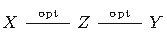
\includegraphics[width=.35\linewidth]{assets/appendixB/figB-1.pdf}
\caption{此图便于表示多个随机变量之间的耦合. 一条边表示对应耦合须最优这一约束. 一般而言，任何由无环图描述的耦合，都可以用粘合引理实现.}\label{fig:B.1}
\end{figure}

\begin{proof}
我们将明确构造这样的三元组$(X,Y,Z)$. 为此，令$Z$服从$\gamma$的第二边缘分布（根据假设，这与$\gamma'$的第一边缘相同）. 那么，$\gamma$和$\gamma'$分别确定给定$Z$时$X$和$Y$的条件分布. 例如，可以在给定$Z$时条件独立地抽取$X,Y$. 这就得到一个有效的三元组$(X,Y,Z)$，见\autoref{fig:B.1}.
\end{proof}


\clearpage\phantomsection\addcontentsline{toc}{section}{参考文献}
\nocite{*}
\bibliographystyle{plain}
\bibliography{bib/references-full}
\index{CAT(0)@CAT(0)|see{非正曲率（NPC）}}
\index{Hadamard@Hadamard|see{非正曲率（NPC）}}
\index{Hellinger–Kantorovich@Hellinger–Kantorovich|see{Wasserstein–Fisher–Rao（WFR）（Wasserstein–Fisher–Rao (WFR)）}}
\index{Kantorovich–Rubinstein distance@Kantorovich–Rubinstein距离（Kantorovich–Rubinstein distance）|see{Wasserstein距离（Wasserstein distance）}}

\printindex
\clearpage
\section*{《数学讲义丛书》编辑方针}\label{sec:publisher-policy}

\noindent\textit{Lecture Notes in Mathematics}\par
\noindent 主编：J.-M. Morel、B. Teissier

\begin{enumerate}
\item 《数学讲义丛书》旨在以迅速、非正式而高水平的方式，报道数学各领域及其应用的新进展. 欢迎分析建模和数值模拟新发展的数学著作.

书稿应当相当自足，内容完整. 因此，它们可以，而且经常不仅介绍作者自己的成果，也介绍他人的相关工作. 书稿可以以专题课程为基础. 此外，书稿还应提供充分的动机、例子与应用. 这使《数学讲义丛书》明显有别于通常十分简洁的期刊论文或技术报告. 那些原拟投期刊、只是篇幅太长而难以被多数期刊接受的文章，通常不具备这种“讲义”性质. 基于类似理由，本丛书通常不接收博士论文，但任教资格论文可能适合.

\item 除专著外，也欢迎由暑期学校或类似强化课程产生的多人合著书稿，前提是这些课程旨在向研究生初级或中级程度的听众介绍活跃的数学主题，并应提供参与者名单.

最终书稿不应只是课程笔记的汇编，而应要求主要讲师事先规划和协调. 全书结构应由主题内容决定，并在科学性导论中说明其动机与安排. 如有可能，编者应统一符号、参考文献、索引与结果的表述. 每篇内容应包含摘要，以及关联其他篇章的引言. 换言之，合著卷册需要的准备工作，远超过将活动期间提交的零散文章简单拼合.

\item 书稿应通过\url{https://www.editorialmanager.com/lnm}在线提交至Springer海德堡数学编辑部，或以电子方式提交给一位丛书编委. 作者应注意，不完整或距离最终稿不够接近的书稿，几乎总会导致更长的审稿时间和仍不明确的审稿建议，从而使最终稿还需再次审阅. 最低限度的材料应包括详细纲要，说明各章拟定内容，并附参考文献与若干样章. LNM审稿期间，不得同时向其他出版者投稿；平行投稿可能导致拒稿.

\item 一般而言，专著会送交至少两位外部审稿人评审. 只有依据完整书稿，才能作出最终出版决定；但旨在形成初步决定的审稿过程，可以以接近最终版本或尚未完成的书稿为基础.

多人合著卷册的分卷编者应安排按通常学术标准对各篇内容进行评审. 若能将审稿报告转交LNM编委会，将十分有帮助. 如果没有转交报告，或者统一性等其他问题仍不明确，丛书编委可能会咨询外部审稿人，对全卷作总体评估.

\item 书稿一般应使用英文提交. 最终稿应包含至少100页数学正文，并且始终包括：
\begin{itemize}
\item 目录；
\item 信息充分的引言，提供足够动机，并可酌情介绍一些历史背景，使不熟悉该主题的读者也能够理解；
\item 主题索引，通常这对读者很有帮助；
\item 为便于评审，书稿应以PDF文件形式提交.
\end{itemize}

\item 精心准备书稿，既能缩短制作周期，也能确保纸质版和在线版具有令人满意的外观. 接收后，作者将被要求准备最终LaTeX源文件（在线模板见\url{https://www.springer.com/gb/authors-editors/book-authors-editors/manuscriptpreparation/5636}）以及相应的PDF文件或压缩PS文件. LaTeX源文件是制作全书在线全文版本所必需的，现有LNM在线卷册见\url{http://link.springer.com/bookseries/304}. 《数学讲义丛书》一卷的技术制作约需12周. 如有必要，可通过\href{mailto:lnm@springer.com}{lnm@springer.com}索取进一步说明.

\item 作者共可获得30册免费样书，并免费访问SpringerLink上的本书，但不收取版税. 若直接从Springer订购供个人使用的Springer图书，可享受33.3\%折扣.

\item 出版承诺通过《出版协议》作出；多人合著卷册的撰稿作者须签署《同意出版书》. Springer-Verlag为每一卷登记版权. 作者可以自由地在后续出版物中再利用其LNM卷册所含材料：仅需书面或电子邮件简要请求正式许可.
\end{enumerate}

\noindent\textbf{联系地址}

\noindent Jean-Michel Morel教授，CMLA，法国卡尚高等师范学校\par
电子邮箱：\href{mailto:moreljeanmichel@gmail.com}{moreljeanmichel@gmail.com}

\noindent Bernard Teissier教授，几何与动力学组，法国巴黎朱西厄数学研究所——巴黎左岸\par
电子邮箱：\href{mailto:bernard.teissier@imj-prg.fr}{bernard.teissier@imj-prg.fr}

\noindent Springer：Ute McCrory，数学编辑部，德国海德堡\par
电子邮箱：\href{mailto:lnm@springer.com}{lnm@springer.com}

\end{document}
